\providecommand{\topdir}{../..} 
\documentclass[\topdir/lecture\_notes.tex]{subfiles}
\graphicspath{{\subfix{./images/}}}

\begin{document}

\section{Financial Assets}
\subsection{Security Markets}
A \emph{financial asset} is defined by the payoffs it provides to its holder. We refer to financial assets with exogenously given payoffs as \emph{securities}.

There are two dates, \(0\) and \(1\). Securities are traded at date \(0\), and their payoffs are realized at date \(1\). Date \(0\), the present, has no uncertainty. On date \(1\), one of \(S\) states can occur.

Security \(j\) is defined by its payoff \(x_{j}\), an element of \(\mathbb{R}^{S}\), where \(x_{js}\) denotes the payoff that the holder of one unit (or one share) of security \(j\) receives in state \(s\) at date \(1\).  Payoffs are in units of the single consumption good available in this economy. The consumption good is therefore the num\'eraire. Payoffs may be positive, zero, or negative. There exists a finite number \(J\) of securities with payoffs \(x_{1}, \ldots, x_{J}\), with \(x_{j} \in \mathbb{R}^{S}\), which are exogenously given.

The \(J \times S\) matrix \(X\) of payoffs of all securities
\[
X=\left[\begin{array}{c}
x_{1} \\
x_{2} \\
\vdots \\
x_{J}
\end{array}\right]
\]
is called the \emph{payoff matrix}. The vectors \(x_{j}\) are understood to be row vectors. In general, vectors are understood to be either row vectors or column vectors, as the context requires.

A \emph{portfolio} consists of holdings in the \(J\) securities. These holdings may be positive, zero, or negative. A positive holding of a security  is called a long position, and a negative holding is called a short position.

A portfolio is denoted by a \(J\)-dimensional vector \(h\), where \(h_{j}\) represents the holdings of security \(j\). The \emph{portfolio payoff} is \(\sum_{j} h_{j} x_{j}\) and can be represented as \(h X\).

The set of payoffs available via trades of securities is the \emph{asset span} and is denoted by \(\mathcal{M}\):
\begin{equation*}
\mathcal{M}=\left\{z \in \mathbb{R}^{S} \colon z=h X \text { for some } h \in \mathbb{R}^{J}\right\} 
\end{equation*}
Thus \(\mathcal{M}\) is the subspace of \(\mathbb{R}^{S}\) spanned by the security payoffs, that is, the row span of the payoff matrix \(X\). If \(\mathcal{M}=\mathbb{R}^{S}\), then markets are \emph{complete}. If \(\mathcal{M}\) is a proper subspace of \(\mathbb{R}^{S}\), then markets are \emph{incomplete}. When markets are complete, any element of \(\mathbb{R}^{S}\) can be obtained as a portfolio payoff.

\begin{theorem}\label{thm:market_completeness}
Markets are complete iff the payoff matrix \(X\) has rank \(S\)\footnote{We use ``\(A\) iff \(B\)'' as an abbreviation for ``\(A\) if and only if \(B\)''. It has the same meaning as ``\(A\) is equivalent to \(B\)'' and as ``\(A\) is a necessary and sufficient condition for \(B\)''. We sometimes use \(A \iff B\) to denote ``\(A\) iff \(B\)''.

Proving necessity in ``\(A\) iff \(B\)'' means proving ``\(B\) implies \(A\)'' (\(B \implies A\)) whereas proving sufficiency means proving ``\(A\) implies \(B\)'' (\(A \implies B\)).
}
\end{theorem}
\begin{proof}
Asset span \(\mathcal{M}\) equals the whole space \(\mathbb{R}^{S}\) iff the equation \(z=h X\), with \(J\) unknowns \(h_{j}\), has a solution for every \(z \in \mathbb{R}^{S}\). A necessary and sufficient condition for this is that \(X\) has rank \(S\).
\end{proof}

A security is called \emph{redundant} if its payoff can be generated as the payoff of a portfolio of other securities. There are no redundant securities iff the payoff matrix \(X\) has rank \(J\).

The prices of securities at date \(0\) are denoted by a \(J\)-dimensional vector \(p=\) \(\left(p_{1}, \ldots, p_{J}\right)\). The price of portfolio \(h\) at security prices \(p\) is \(p h=\sum_{j} p_{j} h_{j}\). The \emph{return} \(r_{j}\) on security \(j\) is its payoff \(x_{j}\) divided by its price \(p_{j}\) (assumed to be nonzero; the return on a payoff with zero price is undefined):
\begin{equation*}
r_{j}=\frac{x_{j}}{p_{j}} 
\end{equation*}
Thus, ``return'' means gross return (``net return'' equals gross return minus one). Throughout, we work with gross returns.

The asset span can be specified using the returns on the securities rather than their payoffs. In this case, the asset span is the subspace of \(\mathbb{R}^{S}\) spanned by the returns on the securities.

The following example illustrates the concepts introduced earlier.
\begin{example} \label{ex:payoff_matrix_example}
Let there be three states and two securities. Security 1 is risk free and has payoff \(x_{1}=(1,1,1)\). Security 2 is risky with \(x_{2}=(1,2,2)\). The payoff matrix is
\begin{align*}
\left[\begin{array}{lll}
1 & 1 & 1 \\
1 & 2 & 2
\end{array}\right]
\end{align*}
The asset span is
\begin{align*}
\mathcal{M}&=\left\{(z_{1}, z_{2}, z_{3}): z_{1}=h_{1}+h_{2}, z_{2}=h_{1}+2 h_{2}, z_{3}=h_{1}+2 h_{2}\text{, for some }(h_{1}, h_{2})\right\},
\end{align*}
which is a two-dimensional subspace of \(\mathbb{R}^{3}\). By inspection, \(\mathcal{M}=\left\{\left(z_{1}, z_{2}, z_{3}\right): z_{2}=z_{3}\right\}\). At prices \(p_{1}=0.8\) and \(p_{2}=1.25\), security returns are \(r_{1}=(1.25,1.25,1.25)\) and \(r_{2}=(0.8,1.6,1.6)\).
\end{example}

\section{Pricing}
\subsection{The Law of One Price}
The \emph{law of one price} says that all portfolios with the same payoff have the same price:
\begin{equation*}
\text { if } h X=h^{\prime} X \text {, then } p h=p h^{\prime}
\end{equation*}
for any two portfolios \(h\) and \(h^{\prime}\).

Because the payoff matrix \(X\) is given exogenously, the law of one price is properly interpreted as a restriction on security prices as opposed to a restriction on payoffs. If there are no redundant securities, only one portfolio can generate any given payoff, and thus the law of one price is trivially satisfied. If there are redundant securities, the law of one price may or may not be satisfied depending on security prices.

A necessary and sufficient condition for the law of one price to hold is that every portfolio with zero payoff has zero price. If the law of one price does not hold, then any payoff (that is, any contingent claim in the asset span) can be purchased at any price.

\subsection{The Payoff Pricing Functional}
For any security prices \(p\) we define a mapping \(q: \mathcal{M} \rightarrow \mathbb{R}\) that assigns to each payoff the price(s) of the portfolio(s) that generate(s) that payoff. Formally,
\begin{equation}
q(z) :=\{w: w=p h \text { for some } h \text { such that } z=h X\}. \label{def:payoff_pricing_functional}
\end{equation}
In general, the mapping \(q\) is a correspondence rather than a single-valued function.

If the law of one price holds, then \(q\) is single valued. Further, it is a linear functional:
\begin{theorem}\label{thm:law_of_one_price_linearity}
The law of one price holds iff \(q\) is a linear functional on the asset span \(\mathcal{M}\).
\end{theorem}
\begin{proof}
If the law of one price holds, then, as just noted, \(q\) is single valued. To prove linearity, consider payoffs \(z, z^{\prime} \in \mathcal{M}\) such that \(z=h X\) and \(z^{\prime}=h^{\prime} X\) for some portfolios \(h\) and \(h^{\prime}\). For arbitrary \(\lambda, \mu \in \mathbb{R}\), the payoff \(\lambda z+\mu z^{\prime}\) can be generated by the portfolio \(\lambda h+\mu h^{\prime}\) with price \(\lambda p h+\mu p h^{\prime}\). Because \(q\) is single valued, Definition \ref{def:payoff_pricing_functional} implies that
\begin{equation*}
q\left(\lambda z+\mu z^{\prime}\right)=\lambda p h+\mu p h^{\prime} . 
\end{equation*}
The right-hand side of the above equation equals \(\lambda q(z)+\mu q\left(z^{\prime}\right)\), and thus \(q\) is linear. Conversely, if \(q\) is a functional, then the law of one price holds by definition.
\end{proof}

Whenever the law of one price holds, we call \(q\) the \emph{payoff pricing functional}.

\subsection{State Prices in Complete Markets}
Let \(e_{s}\) denote the \(s\)th basis vector in the space \(\mathbb{R}^{S}\) of contingent claims, with \(1\) in the \(s\)th place and zeros elsewhere. Vector \(e_{s}\) is the \emph{state claim} or the \emph{Arrow-Debreu security} of state \(s\). It is the claim to one unit of consumption contingent on the occurrence of state \(s\). If markets are complete and if the law of one price holds, then the payoff pricing functional assigns a unique price to each state claim. Let
\begin{equation*}
q_{s} := q(e_{s})
\end{equation*}
denote the price of the state claim of state \(s\). We call \(q_{s}\) the \emph{state price} of state \(s\).

Because any linear functional on \(\mathbb{R}^{S}\) can be identified by its values on the basis vectors of \(\mathbb{R}^{S}\), the payoff pricing functional \(q\) can be represented as
\begin{equation*}
q(z)=q z
\end{equation*}
for every \(z \in \mathbb{R}^{S}\), where \(q\) on the right-hand side of the above equation is an \(S\)-dimensional vector of state prices. With some abuse of notation, we use the same notation for the functional and the vector that represents it.

Because the price of each security equals the value of its payoff under the payoff pricing functional, we have
\begin{equation*}
p_{j}=q x_{j}
\end{equation*}
or, in matrix notation,
\begin{equation}
p=X q \label{eq:security_prices_state_prices}
\end{equation}

Equation (\ref{eq:security_prices_state_prices}) is a system of linear equations that associates state prices with given security prices.

A left inverse of the payoff matrix \(X\) is a matrix \(L\) that satisfies \(L X=I_{S}\), where \(I_{S}\) is the \(S \times S\) identity matrix. A left inverse exists iff \(X\) is of rank \(S\), which occurs if \(J \geq S\) and the columns of \(X\) are linearly independent. Markets are complete iff a left inverse of \(X\) exists.

A matrix \(L\) defined by
\begin{align*}
L=\left(X^{\prime} X\right)^{-1} X^{\prime} 
\end{align*}
where the prime indicates transposition, is a left inverse of \(X\). Thus, \(L\) exists iff \(X^{\prime} X\) is invertible.

Premultiplying both sides of equation (\ref{eq:security_prices_state_prices}) by a left inverse of the payoff matrix, it follows that
\begin{equation*}
q=L p
\end{equation*}
(all left inverses give the same value for \(q\)).

The results of this section depend on the assumption of market completeness because otherwise \(L\) does not exist (or, alternatively, because state claim \(e_{s}\) may not be in the asset span \(\mathcal{M}\), and thus \(q(e_{s})\) may not be defined).

\section{Arbitrage}
\subsection{Notation}
Our convention on inequalities is as follows: for two vectors \(x, y \in \mathbb{R}^{n}\),
\begin{align*}
x & \geq y \text{ means that } x_{i} \geq y_{i} \quad \forall i;&& x \text{ is greater than } y, \\
x & > y \text{ means that } x \geq y \text{ and } x \neq y;&& x \text{ is greater than but not equal to } y, \\
x & \gg y \text{ means that } x_{i}>y_{i} \quad \forall i;&& x \text{ is strictly greater than } y.
\end{align*}
For a vector \(x\), positive means \(x \geq 0\), positive and nonzero means \(x>0\), and strictly positive means \(x \gg 0\). These definitions apply to scalars as well. For scalars, ``positive and nonzero'' is equivalent to ``strictly positive''.

\subsection{Arbitrage and Strong Arbitrage}
A \emph{strong arbitrage} is a portfolio that has a positive payoff and a strictly negative price. An \emph{arbitrage} is a portfolio that is either a strong arbitrage or has a positive and nonzero payoff and zero price. Formally, a strong arbitrage is a portfolio \(h\) that satisfies \(h X \geq 0\) and \(p h<0\), and an arbitrage is a portfolio \(h\) that satisfies \(h X \geq 0\) and \(p h \leq 0\) with either \(h X \neq 0\) or \(p h \neq 0\) (or both).

It is possible for a portfolio to be an arbitrage but not a strong arbitrage:

\begin{example}\label{ex:arbitrage_not_strong}
Let there be two securities with payoffs \(x_{1}=(1,1)\) and \(x_{2}=(1,2)\) and prices \(p_{1}=p_{2}=1\). Then, portfolio \(h=(-1,1)\) is an arbitrage but not a strong arbitrage. In fact, there is no strong arbitrage.
\end{example}

If there exists no portfolio with a positive and nonzero payoff, then any arbitrage is a strong arbitrage. Further, the law of one price does not hold iff there exists a portfolio with zero payoff and strictly negative price. Such a portfolio is a strong arbitrage.

\begin{example}\label{ex:no_positive_payoff}
Suppose that two securities have payoffs \(x_{1}=(-1,2,0)\) and \(x_{2}=\) $(2,2,-1)$. A portfolio \(h=\left(h_{1}, h_{2}\right)\) has a positive payoff if
\begin{gather*}
-h_{1}+2 h_{2} \geq 0 \\
h_{1}+h_{2} \geq 0 
\end{gather*}
and
\begin{equation*}
-h_{2} \geq 0 
\end{equation*}
These inequalities are satisfied by the zero portfolio alone. Therefore, there exists no portfolio with positive and nonzero payoff, implying further that any arbitrage is a strong arbitrage. Because there are no redundant securities, the law of one price holds for any security prices, so there is no strong arbitrage. 

Consequently, there is no arbitrage for any security prices.
\end{example}

\subsection{Visual Representation}
It is helpful to have a visual representation of the set of security prices that exclude arbitrage. Suppose that there are two securities with payoffs \(x_{1}\) and \(x_{2}\), and consider the payoff pairs \(\left(x_{1 s}, x_{2 s}\right)\) in each state. These pairs are denoted \(x_{\cdot 1}, \ldots, x_{\cdot S}\). Figure \ref{fig:positive_payoff_cone} is drawn on the assumption that \(x_{j s}>0\) for all \(j\) and \(s\), but the analysis does not depend on this restriction.

Now interpret the coordinate axes as portfolio weights \(h_{1}\) and \(h_{2}\) so that any point in the diagram is associated with a portfolio \(\left(h_{1}, h_{2}\right)\). For each \(x_{\cdot s}\), construct a line perpendicular to \(x_{\cdot s}\) through the origin. The set of portfolios \(h\) with positive payoff in state \(s\) is the set of points northeast of this line. If this construction is performed in each state, the intersection of the indicated portfolio sets gives the set of portfolios with positive payoffs in all states. The indicated portfolios are those for which the ray through the point \(h\) intersects the arc.

Suppose that security prices are given by \(p=\left(p_{1}, p_{2}\right)\), as shown in figure \ref{fig:negative_price_region}. Then the set of zero-price portfolios consists of the line through the origin perpendicular to \(p\). Figure \ref{fig:no_arbitrage_case}, which combines figures \ref{fig:positive_payoff_cone} and \ref{fig:negative_price_region}, shows that the set of positive-payoff portfolios intersects the set of negative-price portfolios only at the origin, and thus there is no arbitrage.

\begin{figure}
    \begin{center}
        % 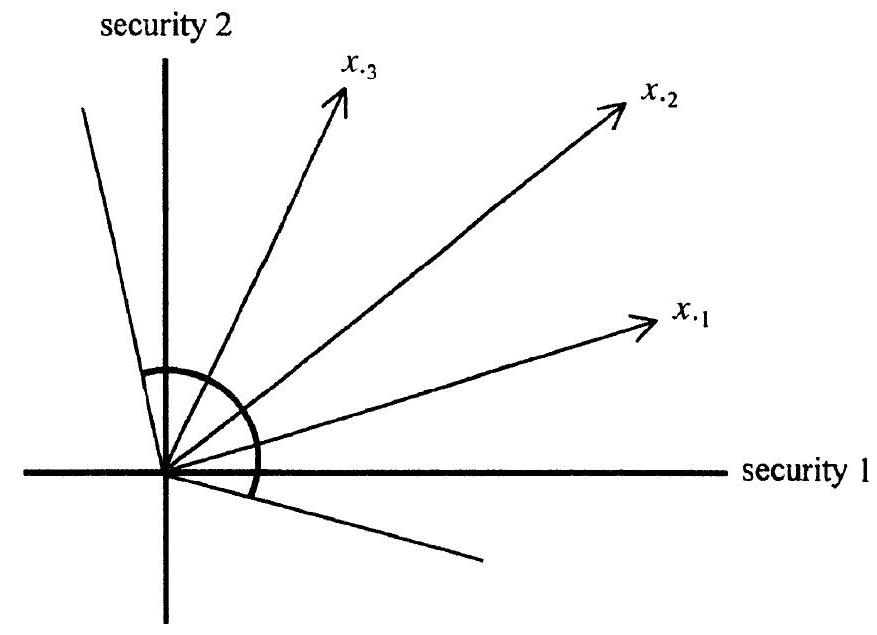
\includegraphics[max width=\textwidth]{2024_03_09_566eeb6d49daa183514ag-054(1)}
          \begin{tikzpicture}[>=Straight Barb,scale=3]
                \pgfmathsetlengthmacro{\angleA}{15}
                \pgfmathsetlengthmacro{\angleB}{45}
                \pgfmathsetlengthmacro{\angleC}{75}
                
                \pgfmathsetlengthmacro{\maxangleA}{\angleA+90}
                \pgfmathsetlengthmacro{\maxangleB}{\angleB+90}
                \pgfmathsetlengthmacro{\maxangleC}{\angleC+90}
                \pgfmathsetlengthmacro{\minangleA}{\angleA-90}
                \pgfmathsetlengthmacro{\minangleB}{\angleB-90}
                \pgfmathsetlengthmacro{\minangleC}{\angleC-90}

%\pgfmathparse{min(3,4,-2,250,-8,100)} \pgfmathresult

                \pgfmathsetlengthmacro{\minperpangle}{max(\minangleA,\minangleB,\minangleC)}
                \pgfmathsetlengthmacro{\maxperpangle}{min(\maxangleA,\maxangleB,\maxangleC)}
                
                \draw[ultra thick,black!20!red](\maxperpangle:1.8)--(0,0)--(\minperpangle:1.8);
                \draw[ultra thick,black!20!red] (0,0) ++( \maxperpangle : 0.5 ) arc ( \maxperpangle:\minperpangle:0.5 );
                \draw[thick,line cap = butt, join=bevel](0,2)node[above]{\small Security 2}--(0,0)--(2,0)node[right]{\small Security 1};
                \foreach \x [count=\xi] in {\angleA,\angleB,\angleC} {
                  \draw[arrow,line cap = round](0,0)--(\x:1.8);
                  \node at (\x:2){\(x_{\cdot \xi}\)};
                }
                
                
        \end{tikzpicture}
    \end{center}
    \caption{The rays labeled \(x_{\cdot 1}, x_{\cdot 2}\), and \(x_{\cdot 3}\) show payoffs of securities 1 and 2 in states 1, 2, and 3. The cone indicated by the red arc and the red rays shows portfolios that have positive payoffs in all states.}
    \label{fig:positive_payoff_cone}
\end{figure}

 
This conclusion is a consequence of the fact that \(p\) lies in the interior of the cone defined by the \(x_{\cdot s}\). If \(p\) lies on the boundary of the cone, then there is an arbitrage, but not a strong one (figure \ref{fig:arbitrage_boundary}), whereas if \(p\) lies outside the cone, then there exists strong arbitrage (figure \ref{fig:strong_arbitrage_case}).

The preceding construction, being two-dimensional, is necessarily restricted to the case in which agents take nonzero positions in at most two securities. It is worth noting that, if there are more than two securities, nonexistence of an arbitrage if portfolios are restricted to contain at most two securities is consistent with existence of an arbitrage if portfolios are unrestricted. This is illustrated by the following example.


\begin{figure}
    \begin{center}
        %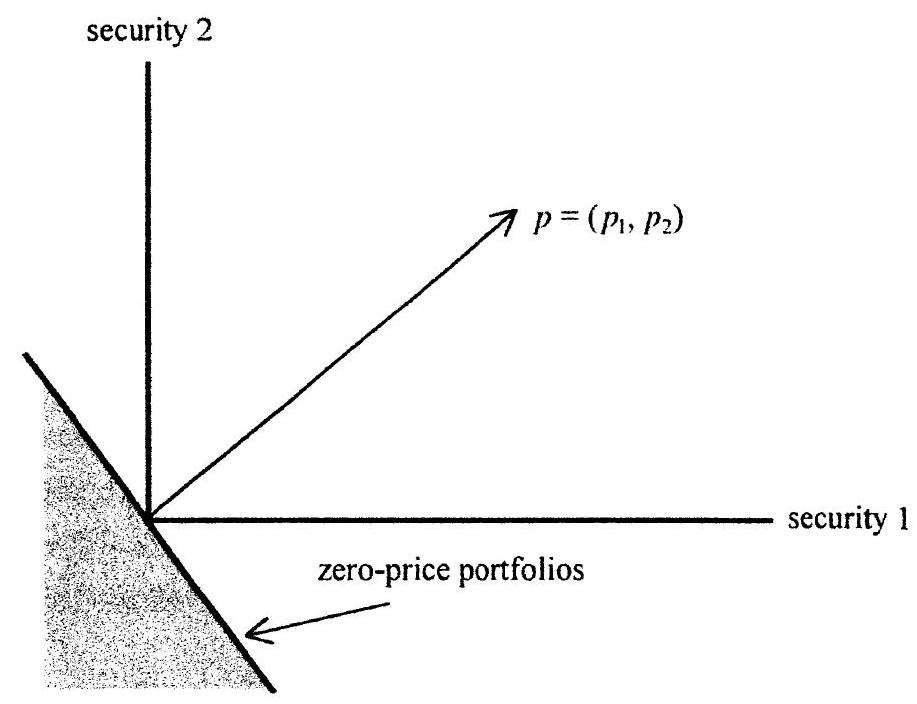
\includegraphics[max width=\textwidth]{2024_03_09_566eeb6d49daa183514ag-054}
                \begin{tikzpicture}[>=Straight Barb,scale=3,
                vert/.style args={of #1 at #2}{insert path={%
                #2 -- (intersection cs:first line={#1}, second line={#2--($#2+(0,10)$)}) }}, vert outwards/.style args={from #1 by #2 on line to #3}{insert path={#1 -- ($#1!#2!90:#3$)}}]
   
                \coordinate (origin) at (0,0);

                \pgfmathsetmacro{\angle}{125}
                \pgfmathsetmacro{\compangle}{\angle-180}
                
                \node[] (A) at (origin) {};
                \node[] (B) at ([shift=({\angle:1 cm})]A) {};
                \node[] (C) at ([shift=({\angle:-1 cm})]A) {};                
                \node[] (D) at (B|-C) {};
                % \node[label={right:\(p=(p_1,p_2)\)},node distance=6.2cm,above right of=A] (P) {};

                \draw[pattern=north east lines](B.center)--(D.center)--(C.center)--(A.center)--(B.center)--cycle;
                %\draw[red] (B) -- ($(A)!(B)!(C)$);
                
                %\node[label={below right:\(C\)}] at (C) {};
                %\draw[red,vert={of {(B)--(C)} at (P)}];
                \draw[arrow,ultra thick,vert outwards={from {($(B)!0.5!(C)$)} by 2cm on line to {(C)}}] node[right=1pt] {\(p=(p_1,p_2)\)};
                \draw[ultra thick,black](\angle:1.1)--(0,0)--(\compangle:1.1);
                \draw[thick,line cap = butt, join=bevel](0,2)node[above]{\small Security 2}--(0,0)--(2,0)node[right]{\small Security 1};

                \node[] (BA) at ($(B)!0.5!(A)$) {};
                %\node[] (AC) at ($(A)!0.5!(C)$) {};
                
                \node[] (label) [above left of=BA,node distance=3cm] {\small zero-price portfolios};
                \draw[thick,->] (label.east) .. controls +(right:0.5cm) and +(up:0cm) .. (BA.north);
                  %\draw[arrow,line cap = round](0,0)--(2:2);
                  %\node at (2.1:2.1){\(p=(p_1,p_2)\)};
        \end{tikzpicture}
    \end{center}
    \caption{Portfolios in the shaded region have a negative price.}
    \label{fig:negative_price_region}
\end{figure}

\begin{figure}
    \begin{center}
        %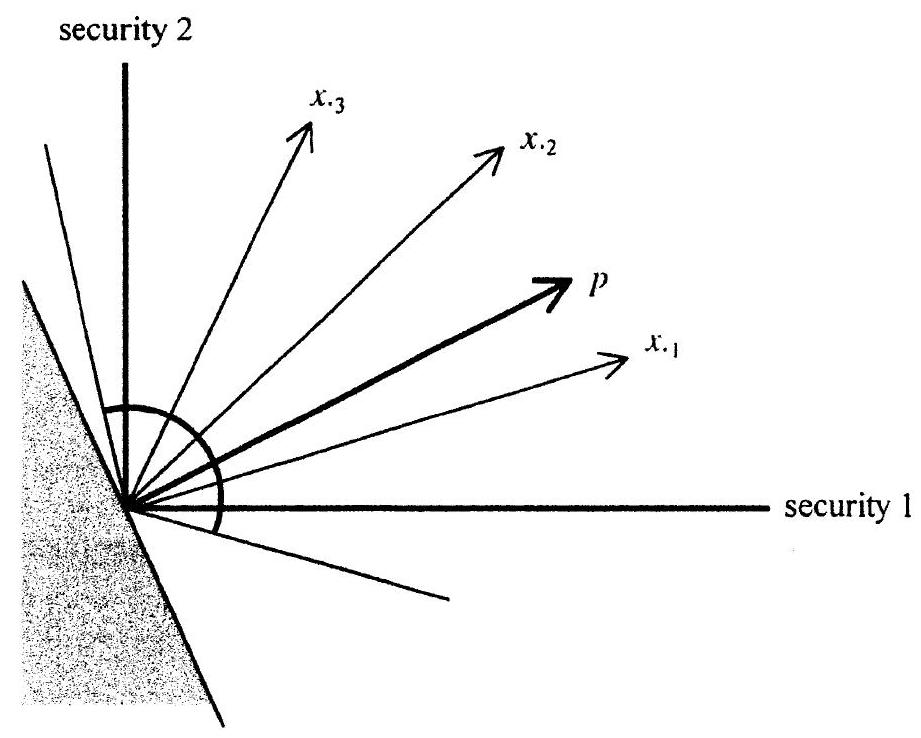
\includegraphics[max width=\textwidth]{2024_03_09_566eeb6d49daa183514ag-055(1)}
                \begin{tikzpicture}[>=Straight Barb,scale=3,
                vert/.style args={of #1 at #2}{insert path={%
                #2 -- (intersection cs:first line={#1}, second line={#2--($#2+(0,10)$)}) }}, vert outwards/.style args={from #1 by #2 on line to #3}{insert path={#1 -- ($#1!#2!90:#3$)}}]


                             \pgfmathsetlengthmacro{\angleA}{15}
                \pgfmathsetlengthmacro{\angleB}{45}
                \pgfmathsetlengthmacro{\angleC}{75}
                
                \pgfmathsetlengthmacro{\maxangleA}{\angleA+90}
                \pgfmathsetlengthmacro{\maxangleB}{\angleB+90}
                \pgfmathsetlengthmacro{\maxangleC}{\angleC+90}
                \pgfmathsetlengthmacro{\minangleA}{\angleA-90}
                \pgfmathsetlengthmacro{\minangleB}{\angleB-90}
                \pgfmathsetlengthmacro{\minangleC}{\angleC-90}

%\pgfmathparse{min(3,4,-2,250,-8,100)} \pgfmathresult

                \pgfmathsetlengthmacro{\minperpangle}{max(\minangleA,\minangleB,\minangleC)}
                \pgfmathsetlengthmacro{\maxperpangle}{min(\maxangleA,\maxangleB,\maxangleC)}
                
                \draw[ultra thick,black!20!red](\maxperpangle:1.8)--(0,0)--(\minperpangle:1.8);
                \draw[ultra thick,black!20!red] (0,0) ++( \maxperpangle : 0.5 ) arc ( \maxperpangle:\minperpangle:0.5 );
                \draw[thick,line cap = butt, join=bevel](0,2)node[above]{\small Security 2}--(0,0)--(2,0)node[right]{\small Security 1};
                \foreach \x [count=\xi] in {\angleA,\angleB,\angleC} {
                  \draw[arrow,line cap = round](0,0)--(\x:1.8);
                  \node at (\x:2){\(x_{\cdot \xi}\)};
                }
                
                \coordinate (origin) at (0,0);

                \pgfmathsetmacro{\angle}{125}
                \pgfmathsetmacro{\compangle}{\angle-180}
                
                \node[] (A) at (origin) {};
                \node[] (B) at ([shift=({\angle:1 cm})]A) {};
                \node[] (C) at ([shift=({\angle:-1 cm})]A) {};                
                \node[] (D) at (B|-C) {};
                % \node[label={right:\(p=(p_1,p_2)\)},node distance=6.2cm,above right of=A] (P) {};

                \draw[pattern=north east lines](B.center)--(D.center)--(C.center)--(A.center)--(B.center)--cycle;
                %\draw[red] (B) -- ($(A)!(B)!(C)$);
                
                %\node[label={below right:\(C\)}] at (C) {};
                %\draw[red,vert={of {(B)--(C)} at (P)}];
                \draw[arrow,ultra thick,vert outwards={from {($(B)!0.5!(C)$)} by 2cm on line to {(C)}}] node[right=1pt] {\(p=(p_1,p_2)\)};
                \draw[ultra thick,black](\angle:1.1)--(0,0)--(\compangle:1.1);


                %\node[] (BA) at ($(B)!0.5!(A)$) {};
                %\node[] (AC) at ($(A)!0.5!(C)$) {};
                
                %\node[] (label) [above left of=BA,node distance=3cm] {\small zero-price portfolios};
                %\draw[thick,->] (label.east) .. controls +(right:0.6cm) and +(up:0.2cm) .. (BA.north);
                  %\draw[arrow,line cap = round](0,0)--(2:2);
                  %\node at (2.1:2.1){\(p=(p_1,p_2)\)};
        \end{tikzpicture}
    \end{center}
    \caption{The portfolios in the cone determined by the red rays have positive payoffs; the portfolios in the shaded region have a negative price. These regions intersect only at the origin, indicating the absence of arbitrage. This conclusion follows from the fact that \(p\) lies in the cone generated by the security payoffs.}
    \label{fig:no_arbitrage_case}
\end{figure}

\begin{example}\label{ex:three_securities_arbitrage}
Consider three securities with payoffs \(x_{1}=(1,1,0), x_{2}=\) $(0,1,1)$, and \(x_{3}=(1,0,1)\) and with prices \(p_{1}=1\), and \(p_{2}=p_{3}=1 / 2\). No arbitrage exists with nonzero positions in any two of these securities, but portfolio \(h=(-1,1,1)\) is an arbitrage.
\end{example}

\begin{figure}
    \begin{center}
        %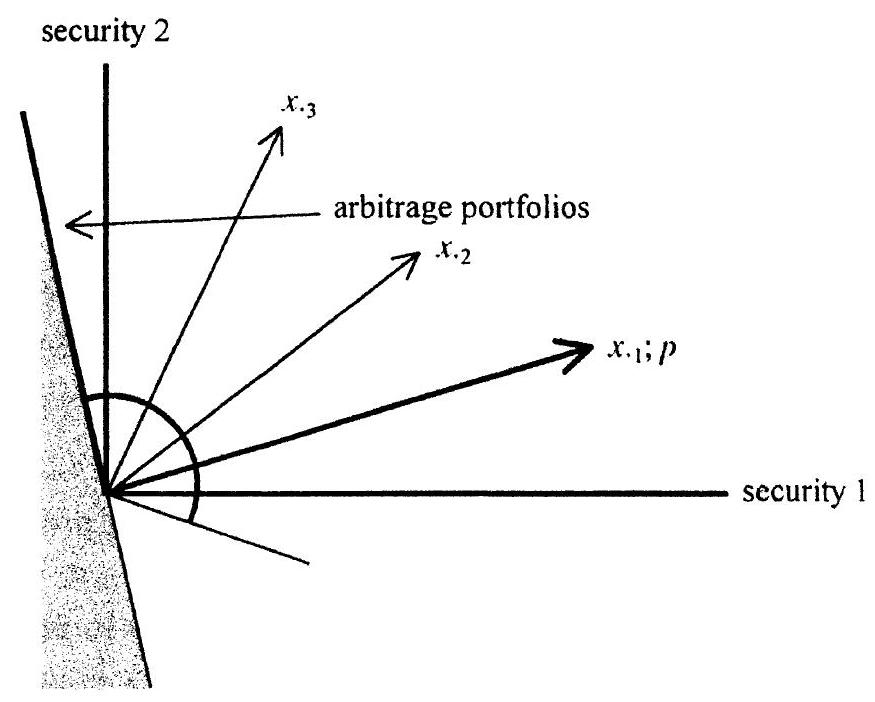
\includegraphics[max width=\textwidth]{2024_03_09_566eeb6d49daa183514ag-055}
         \begin{tikzpicture}[>=Straight Barb,scale=3,
                vert/.style args={of #1 at #2}{insert path={%
                #2 -- (intersection cs:first line={#1}, second line={#2--($#2+(0,10)$)}) }}, vert outwards/.style args={from #1 by #2 on line to #3}{insert path={#1 -- ($#1!#2!90:#3$)}}]


                \pgfmathsetlengthmacro{\angleA}{15}
                \pgfmathsetlengthmacro{\angleB}{45}
                \pgfmathsetlengthmacro{\angleC}{75}
                
                \pgfmathsetlengthmacro{\maxangleA}{\angleA+90}
                \pgfmathsetlengthmacro{\maxangleB}{\angleB+90}
                \pgfmathsetlengthmacro{\maxangleC}{\angleC+90}
                \pgfmathsetlengthmacro{\minangleA}{\angleA-90}
                \pgfmathsetlengthmacro{\minangleB}{\angleB-90}
                \pgfmathsetlengthmacro{\minangleC}{\angleC-90}

%\pgfmathparse{min(3,4,-2,250,-8,100)} \pgfmathresult

                \pgfmathsetlengthmacro{\minperpangle}{max(\minangleA,\minangleB,\minangleC)}
                \pgfmathsetlengthmacro{\maxperpangle}{min(\maxangleA,\maxangleB,\maxangleC)}

                \draw[thick,line cap = butt, join=bevel](0,2)node[above]{\small Security 2}--(0,0)--(2,0)node[right]{\small Security 1};
                \draw[ultra thick,black!20!red] (0,0) ++( \maxperpangle : 0.5 ) arc ( \maxperpangle:\minperpangle:0.5 );
                                
                \foreach \x [count=\xi] in {\angleB,\angleC} {
                  \draw[arrow,line cap = round](0,0)--(\x:1.8);
                  \node at (\x:2){\(x_{\cdot \xi}\)};
                }

                \coordinate (origin) at (0,0);

                \pgfmathsetmacro{\angle}{\maxperpangle}
                \pgfmathsetmacro{\compangle}{\angle-180}
                
                \node[] (A) at (origin) {};
                \node[] (B) at ([shift=({\angle:1.3 cm})]A) {};
                \node[] (C) at ([shift=({\angle:-1 cm})]A) {};                
                \node[] (D) at (B|-C) {};
                % \node[label={right:\(p=(p_1,p_2)\)},node distance=6.2cm,above right of=A] (P) {};
                \draw[ultra thick,black](\angle:1.1)--(0,0)--(\compangle:1.1);
                
                \draw[pattern=north east lines](B.center)--(D.center)--(C.center)--(A.center)--(B.center)--cycle;
                %\draw[red] (B) -- ($(A)!(B)!(C)$);
                
                
                %\node[label={below right:\(C\)}] at (C) {};
                %\draw[red,vert={of {(B)--(C)} at (P)}];
                \draw[arrow,ultra thick,vert outwards={from {($(A)!0!(C)$)} by 2cm on line to {(C)}}] node[right=1pt] {\(x_{\cdot 1}; p\)};


                \draw[ultra thick,bicolor={black}{black!20!red}](\maxperpangle:1.8)--(0,0);
                
                \draw[ultra thick,black!20!red](0,0)--(\minperpangle:1.8);
                

                
                \node[] (BA) at ($(B)!-0.2!(A)$) {};
                %\node[] (AC) at ($(A)!0.5!(C)$) {};
                
                \node[align=left] (label) [below left of=BA,node distance=3cm] {\small arbitrage\\\small portfolios};
                %\draw[thick,->] (label.north) .. controls +(left:0.1cm) and +(up:0.2cm) .. (BA.west);
                \draw[thick,->] (label.north).. controls + (up:0.2cm) .. (BA.west);
                %\node[] (BA) at ($(B)!0.5!(A)$) {};
                %\node[] (AC) at ($(A)!0.5!(C)$) {};
                
                %\node[] (label) [above left of=BA,node distance=3cm] {\small zero-price portfolios};
                %\draw[thick,->] (label.east) .. controls +(right:0.6cm) and +(up:0.2cm) .. (BA.north);
                  %\draw[arrow,line cap = round](0,0)--(2:2);
                  %\node at (2.1:2.1){\(p=(p_1,p_2)\)};
        \end{tikzpicture}
        
    \end{center}
    \caption{The ray \(p\) coincides with one of the boundaries of the cone generated by security payoffs. The interpretation is that there exists arbitrage, but not strong arbitrage.}
    \label{fig:arbitrage_boundary}
\end{figure}



\begin{figure}
    \begin{center}
        %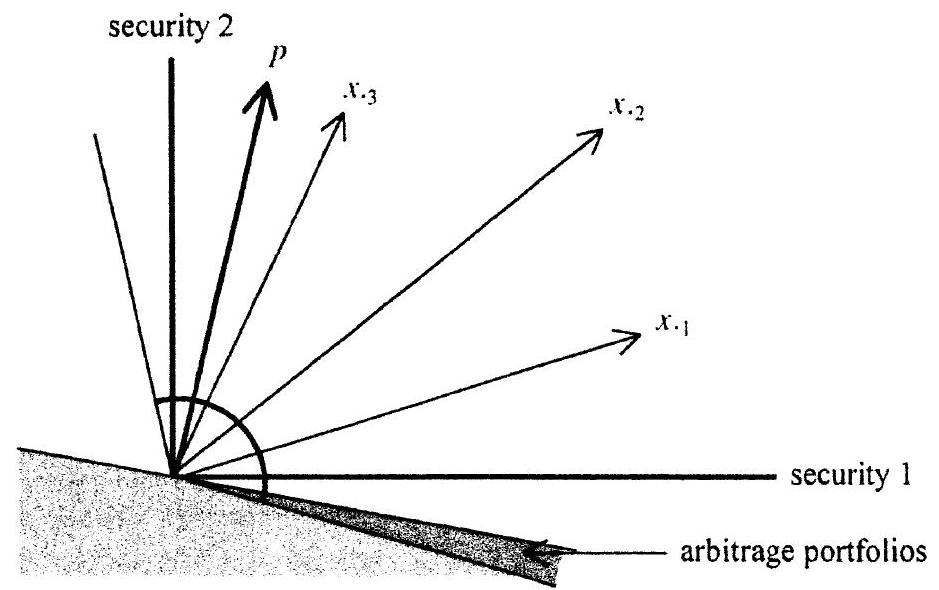
\includegraphics[max width=\textwidth]{2024_03_09_566eeb6d49daa183514ag-056}
          \begin{tikzpicture}[>=Straight Barb,scale=3,
                vert/.style args={of #1 at #2}{insert path={%
                #2 -- (intersection cs:first line={#1}, second line={#2--($#2+(0,10)$)}) }}, vert outwards/.style args={from #1 by #2 on line to #3}{insert path={#1 -- ($#1!#2!90:#3$)}}]


                \pgfmathsetlengthmacro{\angleA}{15}
                \pgfmathsetlengthmacro{\angleB}{45}
                \pgfmathsetlengthmacro{\angleC}{75}
                
                \pgfmathsetlengthmacro{\maxangleA}{\angleA+90}
                \pgfmathsetlengthmacro{\maxangleB}{\angleB+90}
                \pgfmathsetlengthmacro{\maxangleC}{\angleC+90}
                \pgfmathsetlengthmacro{\minangleA}{\angleA-90}
                \pgfmathsetlengthmacro{\minangleB}{\angleB-90}
                \pgfmathsetlengthmacro{\minangleC}{\angleC-90}

%\pgfmathparse{min(3,4,-2,250,-8,100)} \pgfmathresult

                \pgfmathsetlengthmacro{\minperpangle}{max(\minangleA,\minangleB,\minangleC)}
                \pgfmathsetlengthmacro{\maxperpangle}{min(\maxangleA,\maxangleB,\maxangleC)}

                \draw[thick,line cap = butt, join=bevel](0,2)node[above]{\small Security 2}--(0,0)--(2,0)node[right]{\small Security 1};
                \draw[ultra thick,black!20!red] (0,0) ++( \maxperpangle : 0.5 ) arc ( \maxperpangle:\minperpangle:0.5 );
                                
                \foreach \x [count=\xi] in {\angleA, \angleB,\angleC} {
                  \draw[arrow,line cap = round](0,0)--(\x:1.8);
                  \node at (\x:2){\(x_{\cdot \xi}\)};
                }

                \coordinate (origin) at (0,0);

                \pgfmathsetmacro{\angle}{175}
                \pgfmathsetmacro{\compangle}{\angle-180}
                
                \node[] (A) at (origin) {};
                \node[] (B) at ([shift=({\angle:0.3 cm})]A) {};
                \node[] (C) at ([shift=({\angle:-2.1 cm})]A) {};                
                \node[] (D) at (B|-C) {};
                \node[below of = D] (Darb) {};
                \node[]  (Carb) at (C|-Darb) {};
                % \node[label={right:\(p=(p_1,p_2)\)},node distance=6.2cm,above right of=A] (P) {};
                \draw[ultra thick,black](\angle:0.4)--(0,0)--(\compangle:2.1);
                
                \draw[pattern=north east lines](B.center)--(Darb.center)--(Carb.center)--(C.center)--(A.center)--(B.center)--cycle;
                %\draw[red] (B) -- ($(A)!(B)!(C)$);
                
                
                %\node[label={below right:\(C\)}] at (C) {};
                %\draw[red,vert={of {(B)--(C)} at (P)}];
                \draw[arrow,ultra thick,vert outwards={from {($(A)!0!(C)$)} by 1.85cm on line to {(C)}}] node[right=1pt] {\(p\)};

                \draw[ultra thick,black!20!red](\maxperpangle:1.8)--(0,0);
                \draw[ultra thick,black!20!red](0,0)--(\minperpangle:2) node[] (redarb) {};
                
                \draw[fill=red,opacity=0.1](Carb.center)--(C.center)--(A.center)--(redarb.center)--cycle;
                
                %\node[] (BA) at ($(B)!-0.2!(A)$) {};
                \node[] (midAC) at ($(A)!0.7!(C)$) {};
                \node[below right = 0.1cm and 0.1cm of midAC] (AC) {};
                
                \node[align=left] (label) [below right = 0.1cm and 3cm of AC,node distance=3cm] {\small strong\\ \small arbitrage\\\small portfolios};
                %\draw[thick,->] (label.north) .. controls +(left:0.1cm) and +(up:0.2cm) .. (BA.west);
                \draw[thick,->] (label.west)--(AC.east);
                %\node[] (BA) at ($(B)!0.5!(A)$) {};
                %\node[] (AC) at ($(A)!0.5!(C)$) {};
                
                %\node[] (label) [above left of=BA,node distance=3cm] {\small zero-price portfolios};
                %\draw[thick,->] (label.east) .. controls +(right:0.6cm) and +(up:0.2cm) .. (BA.north);
                  %\draw[arrow,line cap = round](0,0)--(2:2);
                  %\node at (2.1:2.1){\(p=(p_1,p_2)\)};
        \end{tikzpicture}
    \end{center}
    \caption{The ray \(p\) lies outside the cone generated by the security payoffs. The portfolios in the indicated region are arbitrages.}
    \label{fig:strong_arbitrage_case}
\end{figure}

\subsection{Positivity of the Payoff Pricing Functional}
A functional is \emph{positive} if it assigns positive value to every positive element of its domain. It is \emph{strictly positive} if it assigns strictly positive value to every positive and nonzero element of its domain. Note that if there is no positive (positive and nonzero) element in the domain of a functional, then the functional is trivially positive (strictly positive). Our terminology of positive and strictly positive functionals is consistent with the terminology of positive and strictly positive vectors in the following sense: a linear functional \(F: \mathbb{R}^{l} \rightarrow \mathbb{R}\) has a representation in the form of a scalar product \(F(x)=f x\) for some vector \(f \in \mathbb{R}^{l}\). Functional \(F\) is strictly positive (positive) iff the corresponding vector \(f\) is strictly positive (positive).

Absence of arbitrage or strong arbitrage at given security prices corresponds to the payoff pricing functional's being strictly positive or positive.

\begin{theorem}
\label{thm:linear}
The payoff pricing functional is linear and strictly positive iff there is no arbitrage.
\end{theorem}
\begin{proof}
The necessity of the absence of arbitrage if the payoff pricing functional is linear and strictly positive is obvious. To prove sufficiency, note that exclusion of arbitrage implies satisfaction of the law of one price, which in turn implies that \(q\) is a linear functional. If \(z \in \mathcal{M}\), then \(q(z)=p h\) for \(h\) such that \(h X=z\). Exclusion of arbitrage implies that \(q(z)>0\), if \(z>0\), and thus \(q\) is strictly positive.
\end{proof}
We also have the following theorem:
\begin{theorem}
\label{thm:positive}
The payoff pricing functional is linear and positive iff there is no strong arbitrage.
\end{theorem}
The proof is similar to that of Theorem \ref{thm:law_of_one_price_linearity}.

\subsection{Positive State Prices}
If markets are complete, then the law of one price implies the existence of a state price vector \(q\) such that
\begin{equation}
p=X q \label{eq:complete_markets_state_price}
\end{equation}
Because the payoff matrix \(X\) is left invertible under complete markets, the vector \(q\) that solves equation (\ref{eq:complete_markets_state_price}) is unique. In view of
\begin{equation*}
q(z)=q z 
\end{equation*}
the absence of arbitrage is equivalent to state prices being strictly positive $(q \gg 0)$, and the absence of strong arbitrage is equivalent to those prices being positive $(q \geq 0)$.

\section{Valuation}
We have already established that security prices can be characterized by a payoff pricing functional mapping the asset span into the reals. The payoff pricing functional is linear and strictly positive (positive) iff security prices exclude arbitrage (strong arbitrage). With complete markets, the payoff pricing functional is uniquely determined, implying the uniqueness of state prices. 

To study incomplete markets, we use a \emph{valuation functional}, an extension of the payoff pricing functional from the asset span \(\mathcal{M}\) to the entire contingent claim space \(\mathbb{R}^{S}\). Thus, a valuation functional is a linear functional
\begin{equation*}
Q: \mathbb{R}^{S} \rightarrow \mathbb{R} 
\end{equation*}
that coincides with the payoff pricing functional on the asset \(\operatorname{span} \mathcal{M}\); that is,
\begin{equation*}
Q(z)=q(z) \quad \text { for every } z \in \mathcal{M}. 
\end{equation*}

A valuation functional assigns values to all contingent claims, not just to payoffs. Of special interest is a valuation functional that is strictly positive (positive) because, in the case of complete markets, this property is equivalent to the absence of arbitrage (strong arbitrage).

The following simple example illustrates a positive valuation functional.

\begin{example} \label{ex:positive_valuation_functional}
Suppose that there are two states and a single security with payoff \(x_{1}=(1,2)\) and price \(p_{1}=1\). The asset span is \(\mathcal{M}=\operatorname{span}\{(1,2)\}=\{(\alpha, 2 \alpha) \colon \alpha \in \mathbb{R}\}\), and the payoff pricing functional is given by \(q(\alpha, 2 \alpha)=\alpha\). Each functional \(Q \colon \mathbb{R}^{2} \rightarrow \mathbb{R}\) defined by \(Q(z)=q_{1} z_{1}+q_{2} z_{2}\), where \(q_{1}, q_{2} \geq 0\) and \(q_{1}+2 q_{2}=1\) is a positive valuation functional.
\end{example}

\subsection{The Fundamental Theorem of Finance}
If we consider an arbitrary vector of security prices, can we be assured that a strictly positive (positive) valuation functional exists? It cannot exist if security prices permit arbitrage (strong arbitrage) because then either the payoff pricing functional does not exist or it is not strictly positive (positive).

We come now to a critical question: If security prices are such as to exclude arbitrage, does a strictly positive valuation functional exist? The answer is provided in the following theorem.

\begin{theorem}[Fundamental Theorem of Finance]\label{thm:fundamental_theorem_finance}
Security prices exclude arbitrage iff there exists a strictly positive valuation functional.
\end{theorem}
Suppose now only that security prices exclude strong arbitrage. This weakening of the condition implies a weakening of the conclusion:

\begin{theorem}[Fundamental Theorem of Finance, Weak Form]\label{thm:fundamental_theorem_finance_weak}
Security prices exclude strong arbitrage iff there exists a positive valuation functional.
\end{theorem}

For both theorems, necessity follows from Theorems \ref{thm:law_of_one_price_linearity} and \ref{thm:positive} because existence of a strictly positive (positive) valuation functional implies existence of a strictly positive (positive) payoff pricing functional, the payoff pricing functional being a restriction of the valuation functional. 

The proof of sufficiency is more involved. The extension of the payoff pricing functional \(q\) from the asset span to the entire commodity space is achieved by extending \(q\) one dimension at a time. In the first step we choose a contingent claim \(\hat{z}\) not in the asset span \(\mathcal{M}\) and extend \(q\) to the subspace spanned by \(\mathcal{M}\) and \(\hat{z}\). This extended subspace has dimension equal to the dimension of \(\mathcal{M}\) plus one. The extension of the payoff pricing functional is achieved by specifying a value \(\pi\) for the contingent claim \(\hat{z}\). For the extension to remain strictly positive (positive), the chosen value \(\pi\) must be such that all payoffs greater than \(\hat{z}\) have prices that are strictly greater (greater) than \(\pi\), and all payoffs less than \(\hat{z}\) have prices that are strictly less (less) than \(\pi\). These restrictions define an interval in which \(\pi\) must lie. The extension is the payoff pricing functional for security markets consisting of \(J\) securities with payoffs \(\left\{x_{1}, \ldots, x_{J}\right\}\) and prices \(\left\{p_{1}, \ldots, p_{J}\right\}\) and a security with payoff \(\hat{z}\) and price \(\pi\).

In the second step, we choose a contingent claim not in the span of the \(J+1\) securities of step 1 and extend the payoff pricing functional to the subspace spanned by the \(J+1\) securities of step 1 and the new contingent claim. After \(S-J\) steps we achieve an extension to the entire commodity space.

The formal proof is provided below as optional.

\begin{optional}
\subsection{Proof of Sufficiency in the Fundamental Theorem of Finance}
Because all of the steps in the construction of the extension are the same, we present only the first one.
\subsubsection*{Bounds on the Values of Contingent Claims}
We now define the upper and lower bounds on the value of a contingent claim \(z \in \mathbb{R}^{S}\) that can be inferred from the prices of the payoffs in \(\mathcal{M}\). The upper bound
\begin{equation}
q_{u}(z) := \min _{h}\{p h: h X \geq z\} \label{4.3}
\end{equation}
is the lowest price of a portfolio, the payoff of which dominates the contingent claim. If such a portfolio does not exist, we set \(q_{u}(z)=+\infty\). For example, if \(\mathcal{M}=\operatorname{span}\{(1,0)\}\) and \(z=(1,1)\), then \(q_{u}(z)=+\infty\).

The lower bound
\begin{equation}
q_{\ell}(z) := \max _{h}\{p h: h X \leq z\} \label{4.4}
\end{equation}
is the highest price of a portfolio, the payoff of which is dominated by the contingent claim. If such a portfolio does not exist, we set \(q_{\ell}(z)=-\infty\). For example, if \(\mathcal{M}=\operatorname{span}\{(1,0)\}\) and \(z=(-1,-1)\), then \(q_{\ell}(z)=-\infty\).

For a contingent claim in the asset span, the lower and the upper bounds coincide with the value under the payoff pricing functional as long as there exists no strong arbitrage:

\begin{proposition} \label{prop:bounds_equal_pricing}
If security prices exclude strong arbitrage, then \(q_{u}(z)=q_{\ell}(z)=\) \(q(z)\) for every \(z \in \mathcal{M}\).
\end{proposition}
\begin{proof}
By the definitions of the bounds we have \(q_{u}(z) \leq q(z)\) and \(q_{\ell}(z) \geq q(z)\) for \(z \in \mathcal{M}\). Suppose that \(q_{u}(z)<q(z)\) for some \(z \in \mathcal{M}\). Then \(q_{u}(z)<+\infty\) and there exists a portfolio \(h^{\prime}\) such that
\begin{equation*}
h^{\prime} X \geq z 
\end{equation*}
and
\begin{equation*}
p h^{\prime}<q(z) . 
\end{equation*}
Let \(h\) be a portfolio such that \(h X=z\) and \(p h=q(z)\). Then portfolio \(h^{\prime}-h\) is a strong arbitrage. This contradicts the assumption. The proof that \(q_{\ell}(z)=q(z)\) is similar.
\end{proof}

The following two examples illustrate the bounds on the values of contingent claims that are not in the asset span.

\begin{example}\label{ex:call_option_bounds_simple}
In Example \ref{ex:positive_valuation_functional}, the contingent claim \(z=(1,1)\) is not in the asset span. We have
\begin{align}
& q_{u}(z)=\min \{h:(h, 2 h) \geq(1,1)\}=1 \label{4.7}\\
& q_{\ell}(z)=\max \{h:(h, 2 h) \leq(1,1)\}=\frac{1}{2} . \label{4.8}
\end{align}
Thus the bounds on the value of \(z\) are \(1 / 2\) and 1.
\end{example}
\begin{example}\label{ex:call_option_bounds_detailed}
Let there be two securities: security 1, a bond with risk-free payoff \(x_{1}=(1,1,1)\), and security 2 , a stock with payoff \(x_{2}=(1,2,4)\). The prices of the bond and stock are, respectively, \(p_{1}=1 / 2\) and \(p_{2}=1\). A nontraded call option on the stock with a strike price of 3 has the payoff \(z=(0,0,1)\). That payoff is not in the span of the payoffs on the stock and the bond and hence cannot be priced using the payoff pricing functional.

A lower bound on the value of the call is determined by solving
\begin{equation}
\max _{h_{1}, h_{2}}\left(p_{1} h_{1}+p_{2} h_{2}\right) \label{eq:call_lower_bound}
\end{equation}
subject to
\begin{equation*}
h_{1} x_{1}+h_{2} x_{2} \leq z 
\end{equation*}
The constraint implies that \(h_{1}\) and \(h_{2}\) satisfy
\begin{align}
& h_{1}+h_{2} \leq 0, \label{eq:call_constraint_1}\\
& h_{1}+2 h_{2} \leq 0, \label{eq:call_constraint_2}\\
& h_{1}+4 h_{2} \leq 1 . \label{eq:call_constraint_3}
\end{align}

The linear program (\ref{eq:call_lower_bound}) can easily be solved graphically.

One can also argue as follows: because there are two choice variables, it is permissible to assume that at the solution at least two of the constraints are satisfied with equality. Constraints (\ref{eq:call_constraint_1}) and (\ref{eq:call_constraint_2}) are satisfied at equality by \(h_{1}=h_{2}=0\), at which point constraint (\ref{eq:call_constraint_3}) is satisfied. Constraints (\ref{eq:call_constraint_1}) and (\ref{eq:call_constraint_3}) are satisfied at equality by \(h_{1}=-1 / 3, h_{2}=1 / 3\), at which point constraint (\ref{eq:call_constraint_2}) is violated. Constraints (\ref{eq:call_constraint_2}) and (\ref{eq:call_constraint_3}) are satisfied at equality by \(h_{1}=-1, h_{2}=1 / 2\), at which point constraint (\ref{eq:call_constraint_1}) is satisfied.

The two points at which two of the constraints are satisfied as equalities and the third constraint is satisfied both give portfolios with zero price, and thus zero is the lower bound for the value of the call.

The upper bound on the value of the call is determined by solving
\begin{equation*}
\min _{h_{1}, h_{2}}\left(p_{1} h_{1}+p_{2} h_{2}\right) 
\end{equation*}
subject to
\begin{align}
& h_{1}+h_{2} \geq 0, \label{eq:call_constraint_4}\\
& h_{1}+2 h_{2} \geq 0, \label{eq:call_constraint_5}\\
& h_{1}+4 h_{2} \geq 1 . \label{eq:call_constraint_6}
\end{align}

As earlier, the minimum is attained at a point at which at least two of the constraints are satisfied with equality. Because constraints (\ref{eq:call_constraint_4})-(\ref{eq:call_constraint_6}) are the reverse inequalities to (\ref{eq:call_constraint_1})-(\ref{eq:call_constraint_3}), the only point that satisfies two of the constraints with equality is \(h_{1}=-1 / 3, h_{2}=1 / 3\). The price of this portfolio is \(1 / 6\). Thus, the bounds on the value of the call option are zero and \(1 / 6\).
\end{example}
Important properties of the bounds \(q_{\ell}\) and \(q_{u}\) are given in the following propositions.

\begin{proposition} \label{prop:bounds_ordering}
If security prices exclude strong arbitrage, then \(q_{u}(z) \geq q_{\ell}(z)\) for every contingent claim \(z \in \mathbb{R}^{S}\). Further, \(q_{u}(z)>-\infty\) and \(q_{\ell}(z)<+\infty\) for every \(z \in \mathbb{R}^{S}\).
\end{proposition}
\begin{proof}
Suppose that \(q_{u}(z)<q_{\ell}(z)\) for some \(z \in \mathbb{R}^{S}\). Then \(q_{u}(z)<+\infty\) and \(q_{\ell}(z)>-\infty\), and there exist portfolios \(h^{\prime}\) and \(h^{\prime \prime}\) such that
\begin{equation*}
h^{\prime} X \leq z \leq h^{\prime \prime} X 
\end{equation*}
and
\begin{equation*}
p h^{\prime}>p h^{\prime \prime} . 
\end{equation*}
But then the portfolio \(h^{\prime \prime}-h^{\prime}\) satisfies \(\left(h^{\prime \prime}-h^{\prime}\right) X \geq 0\) and \(p\left(h^{\prime \prime}-h^{\prime}\right)<0\), and thus it is a strong arbitrage. This contradicts the assumption.

As to the second part, we can assume that there are no redundant securities. If there are redundant securities, the absence of arbitrage implies that the law of one price holds, and the payoff pricing functional and the upper and lower bounds in the markets with a smaller subset of nonredundant securities are the same as with the full set of securities.

Suppose by contradiction that \(q_{u}(z)=-\infty\) for some \(z \in \mathbb{R}^{S}\). Then there exists a sequence of portfolios \(\left\{h^{n}\right\}\) such that
\begin{equation}
h^{n} X \geq z \label{4.20}
\end{equation}
and
\begin{equation}
\lim _{n \rightarrow \infty} p h^{n}=-\infty . \label{4.21}
\end{equation}

Equation (\ref{4.21}) implies that sequence \(\left\{h^{n}\right\}\) is unbounded, that is, \(\lim \left\|h^{n}\right\|=+\infty\) where \(\left\|h^{n}\right\|\) denotes the Euclidean norm of \(h^{n}\). Consider the bounded sequence \(\left\{h^{n} /\left\|h^{n}\right\|\right\}\) and its nonzero limit \(\hat{h}\). Dividing both sides of inequality (\ref{4.20}) by \(\left\|h^{n}\right\|\) and taking limits as \(n\) goes to infinity, we obtain
\begin{equation}
\hat{h} X \geq 0 \text {. } \label{4.22}
\end{equation}
Further, equation (\ref{4.21}) implies that
\begin{equation}
p \hat{h} \leq 0 . \label{4.23}
\end{equation}

Because portfolio \(\hat{h}\) is nonzero and there are no redundant securities, its payoff is nonzero and inequalities (\ref{4.22}) and (\ref{4.23}) imply that \(\hat{h}\) is an arbitrage. This is a contradiction.

The proof that \(q_{\ell}(z)<+\infty\) is similar.
\end{proof}

Also we have the following proposition.

\begin{proposition} \label{prop:bounds_strict_inequality}
If security prices exclude arbitrage, then \(q_{u}(z)>q_{\ell}(z)\) for every contingent claim \(z\) not in the asset span.
\end{proposition}
\begin{proof}
In view of Proposition \ref{prop:bounds_ordering}, we only have to prove that \(q_{u}(z) \neq q_{\ell}(z)\) for every \(z \notin \mathcal{M}\). Suppose that \(q_{u}(z)=q_{\ell}(z)\) for some \(z \notin \mathcal{M}\). It follows from the second part of Proposition \ref{prop:bounds_ordering} that \(q_{u}(z)<+\infty\) and \(q_{\ell}(z)>-\infty\). Therefore there exist portfolios \(h^{\prime}\) and \(h^{\prime \prime}\) such that
\begin{equation}
h^{\prime} X \leq z \leq h^{\prime \prime} X \label{4.24}
\end{equation}
and
\begin{equation*}
p h^{\prime}=p h^{\prime \prime}=q_{u}(z) 
\end{equation*}

Neither of the weak inequalities in expression (\ref{4.24}) can be an equality because \(z\) is not in the asset span; that is, it cannot be generated by a portfolio. Consequently, \(\left(h^{\prime \prime}-h^{\prime}\right) X>0\), and \(p\left(h^{\prime \prime}-h^{\prime}\right)=0\), and thus the portfolio \(h^{\prime \prime}-h^{\prime}\) is an arbitrage. This is a contradiction.
\end{proof}

\subsubsection*{The Extension}
Having derived upper and lower bounds on the value of any contingent claim, we turn now to how these bounds are used to extend the payoff pricing functional.

Fix a contingent \(\operatorname{claim} \hat{z} \notin \mathcal{M}\). Define \(\mathcal{N}\) by
\begin{equation*}
\mathcal{N}=\{z+\lambda \hat{z}: z \in \mathcal{M} \text { and } \lambda \in \mathbb{R}\} 
\end{equation*}
Thus \(\mathcal{N}\) is the subspace of \(\mathbb{R}^{S}\) that has dimension equal to the dimension of \(\mathcal{M}\) plus one and contains \(\mathcal{M}\) and \(\hat{z}\). It is the asset span of \(J+1\) securities with payoffs \(\left\{x_{1}, \ldots, x_{J}\right\}\) and \(\hat{z}\).

If there is no strong arbitrage -- equivalently, if the payoff pricing functional \(q\) is positive -- then Proposition \ref{prop:bounds_ordering} implies that a finite value \(\pi\) can be chosen to satisfy
\begin{equation*}
q_{\ell}(\hat{z}) \leq \pi \leq q_{u}(\hat{z}) . 
\end{equation*}
We extend \(q\) to a linear functional on \(\mathcal{N}\) in that we define \(Q: \mathcal{N} \rightarrow \mathbb{R}\) by
\begin{equation}
Q(z+\lambda \hat{z}) := q(z)+\lambda \pi . \label{4.28}
\end{equation}
We now prove that \(Q\), as just defined, is the desired positive extension of \(q\).

\begin{proposition} \label{prop:extension_positive}
If \(q: \mathcal{M} \rightarrow \mathbb{R}\) is positive, so is \(Q: \mathcal{N} \rightarrow \mathbb{R}\).
\end{proposition}
\begin{proof}
Let \(y \in \mathcal{N}\). Then
\begin{equation*}
y=z+\lambda \hat{z} 
\end{equation*}
for some \(z \in \mathcal{M}\) and some \(\lambda \in \mathbb{R}\). Of the three possibilities for \(\lambda\), suppose first that \(\lambda>0\). Then \(y \geq 0\) implies
\begin{equation}
\hat{z} \geq-\frac{z}{\lambda} . \label{4.30}
\end{equation}
If we apply \(q_{\ell}\) to both sides of inequality (\ref{4.30}) and use the implication of definition (\ref{4.4}) that \(q_{\ell}\) is an increasing function, the result is
\begin{equation}
q_{\ell}(\hat{z}) \geq q_{\ell}\left(-\frac{z}{\lambda}\right) \label{4.31}
\end{equation}
By Proposition \ref{prop:bounds_equal_pricing}, the functions \(q\) and \(q_{\ell}\) coincide on \(\mathcal{M}\). Because \(-z / \lambda \in \mathcal{M}\), we have \(q_{\ell}(-z / \lambda)=q(-z / \lambda)\). Therefore, inequality (\ref{4.31}) becomes
\begin{equation}
q_{\ell}(\hat{z}) \geq q\left(-\frac{z}{\lambda}\right) \label{4.32}
\end{equation}
Because \(\pi \geq q_{\ell}(\hat{z})\), inequality (\ref{4.32}) implies that
\begin{equation*}
\pi \geq q\left(-\frac{z}{\lambda}\right) 
\end{equation*}
or alternatively that
\begin{equation}
q(z)+\lambda \pi \geq 0 . \label{4.34}
\end{equation}

Because the left-hand side of inequality (\ref{4.34}) equals \(Q(y)\), we obtain that \(Q(y) \geq 0\).

If \(\lambda<0\), a similar argument, but using \(q_{u}\) and the fact that \(\pi \leq q_{u}(\hat{z})\), also gives \(Q(y) \geq 0\). Finally, if \(\lambda=0\), then \(y=z\) and \(Q(y)=q(z)\). The positivity of \(q\) implies that if \(y \geq 0\), then \(Q(y) \geq 0\).
\end{proof}
If there is no arbitrage --- equivalently, if \(q\) is strictly positive --- then Proposition \ref{prop:bounds_strict_inequality} implies that \(\pi\) can be chosen to satisfy
\begin{equation*}
q_{\ell}(\hat{z})<\pi<q_{u}(\hat{z}) . 
\end{equation*}
Then the following holds true.
\begin{proposition} \label{prop:extension_strictly_positive}If \(q: \mathcal{M} \rightarrow \mathbb{R}\) is strictly positive, so is \(Q: \mathcal{N} \rightarrow \mathbb{R}\).
\end{proposition}
The proof is essentially the same as the proof of Proposition \ref{prop:extension_positive}.

For the prices \(\left\{p_{1}, \ldots, p_{J}\right\}\) and \(\pi\), functional \(Q\), as defined in equation (\ref{4.28}), is the payoff pricing functional on \(\mathcal{N}\). Therefore \(Q\) is strictly positive (positive) on \(\mathcal{N}\) iff the indicated prices exclude arbitrage (strong arbitrage) in \(J+1\) securities markets with payoffs \(\left\{x_{1}, \ldots, x_{J}\right\}\) and \(\hat{z}\).
\begin{example}\label{ex:extension_example}
In example \ref{ex:call_option_bounds_simple}, define
\begin{equation*}
\mathcal{N}=\{z+\lambda \hat{z}: z \in \mathcal{M}, \lambda \in \mathbb{R}\} 
\end{equation*}
where \(\mathcal{M}=\operatorname{span}\{(1,2)\}\), and \(\hat{z}=(1,1)\). Thus \(\mathcal{N}=\mathbb{R}^{2}\). We have the following bounds on the value \(\pi\) of \(\hat{z}\) (see equations (\ref{4.7}) and (\ref{4.8})):
\begin{equation*}
\frac{1}{2} \leq \pi \leq 1 
\end{equation*}
We choose \(\pi=3 / 4\) and define \(Q: \mathcal{N} \rightarrow \mathbb{R}\) by
\begin{equation*}
Q(z+\lambda \hat{z})=q(z)+\frac{3}{4} \lambda 
\end{equation*}
for \(z \in \mathcal{M}\) and \(\lambda \in \mathbb{R}\). Recall that \(q(z)=\alpha\) for \(z=(\alpha, 2 \alpha)\). One can easily check that
\begin{equation*}
Q(1,0)=\frac{1}{2} \quad \text { and } \quad Q(0,1)=\frac{1}{4} 
\end{equation*}
and hence that
\begin{equation*}
Q\left(y_{1}, y_{2}\right)=\frac{1}{2} y_{1}+\frac{1}{4} y_{2} 
\end{equation*}
Thus, \(Q\) is strictly positive.
\end{example}
\end{optional}

\subsection{Uniqueness of the Valuation Functional}
Extending the payoff pricing functional into a valuation functional does not result in a unique valuation functional when markets are incomplete. When markets are incomplete, if security prices exclude arbitrage, then there exists a continuum of values of \(\pi\) that define strictly positive extensions.

When markets are complete, the asset span \(\mathcal{M}\) equals the contingent claim space \(\mathbb{R}^{S}\), and the payoff pricing functional is the valuation functional. It turns out that this is the only case of a unique strictly positive valuation functional.

\begin{theorem}\label{thm:valuation_uniqueness}
Suppose that security prices exclude arbitrage. Then security markets are complete iff there exists a unique strictly positive valuation functional.
\end{theorem}
\begin{proof}
The sufficiency of market completeness for the uniqueness of the valuation operator is obvious. Necessity follows from Proposition \ref{prop:bounds_strict_inequality}. If markets are not complete, so that there exists a contingent claim not in the asset span, then there exists a nondegenerate interval of values of that contingent claim that gives rise to different strictly positive valuation functionals.
\end{proof}
Theorem \ref{thm:valuation_uniqueness} does not extend to security prices that exclude strong arbitrage, but do not exclude arbitrage.
\begin{example}\label{ex:zero_price_security}
Suppose that there are two states and a single risk-free security with payoff \(x_{1}=(1,1)\) and price \(p_{1}=0\). Markets are incomplete in this example, and security prices exclude strong arbitrage, but they permit arbitrage. The payoff pricing functional is the zero functional on the asset span \(\mathcal{M}=\{(\alpha, \alpha) \colon \alpha \in \mathbb{R}\}\). Further, the upper and the lower bounds on the value of any contingent claim in \(\mathbb{R}^{2}\) are zero. Therefore, the only positive extension of the payoff pricing functional is the zero functional on \(\mathbb{R}^{2}\). Thus we have uniqueness of the valuation operator without complete markets.
\end{example}

\section{State Prices and Risk-Neutral Probabilities}
\subsection{Introduction}
By the fundamental theorem of finance, the payoff pricing functional can be extended to a strictly positive (positive) valuation functional iff security prices exclude arbitrage (strong arbitrage). We now show that each strictly positive (positive) valuation functional can be represented by a vector of strictly positive (positive) state prices. State prices can easily be calculated as a strictly positive (positive) solution to a system of linear equations relating security prices and their payoffs. An implication of the existence of strictly positive (positive) state prices is the absence of arbitrage (strong arbitrage). An implication of the uniqueness of state prices is that markets are complete.

The valuation functional can also be represented by strictly positive (positive) probabilities of the states. These probabilities, known as risk-neutral probabilities, are simple transforms of the state prices and therefore are just as useful as those prices. Under the risk-neutral probabilities representation, the price of each security equals its expected payoff discounted by the risk-free return.

\subsection{State Prices}
If markets are complete, the payoff pricing functional \(q\) is defined on the entire contingent claim space \(\mathbb{R}^{S}\), and the state price vector \(q=(q_{1}, \ldots, q_{S})\) provides a representation of the functional \(q\) as \(q(z)=q z\) for every payoff \(z \in \mathbb{R}^{S}\). We now extended the same kind of representation to incomplete markets using the valuation functional rather than the payoff pricing functional.

A valuation functional, being a linear functional on \(\mathbb{R}^{S}\), can be identified by its values on the basis vectors of that space. Let
\begin{equation}
q_{s} := Q(e_{s}) \label{eq:state_price_definition} 
\end{equation}
for every \(s\), where \(e_{s}\) is the state claim for state \(s\). The value \(q_{s}\) is the \emph{state price} of state \(s\). If \(Q\) is strictly positive (positive), then each state price \(q_{s}\) is strictly positive (positive).

Because every contingent claim \(z \in \mathbb{R}^{S}\) can be written as \(z=\sum_{s} z_{s} e_{s}\), we have
\begin{equation}
Q(z)=\sum_{s} z_{s} Q(e_{s})=\sum_{s} z_{s} q_{s} 
\end{equation}
or
\begin{equation}
Q(z)=q z. \label{eq:state_price_representation} 
\end{equation}
Equation (\ref{eq:state_price_representation}) is the state-price representation of the valuation functional \(Q\). It defines a one-to-one relation between valuation functionals and state-price vectors. Because the valuation functional in incomplete markets is not unique (Theorem \ref{thm:valuation_uniqueness}), state prices are not unique either.

Equation (\ref{eq:state_price_representation}) provides a simple method for pricing payoffs without determining a portfolio that generates the payoff under consideration. Once state prices are known, the price of every payoff can be obtained. Equation (\ref{eq:state_price_representation}) can also be applied to contingent claims not in the asset span, although for any such claim the derived value will depend on the state-price vector used. It follows from the proof of the fundamental theorem of finance that the derived value is independent of the state-price vector iff the contingent claim lies in the asset span.

State prices can be characterized as solutions to a system of linear equations just as under complete markets. To see this we apply equation (\ref{eq:state_price_representation}) to the payoff \(x_{j}\) of security \(j\). Because \(Q(x_{j})=p_{j}\), we obtain
\begin{equation}
p_{j}=q x_{j}, \label{5.2}
\end{equation}
or in vector-matrix notation
\begin{equation}
p=X q \label{5.4}
\end{equation}
State prices are a solution to the system of \(J\) equations (\ref{5.4}) with \(S\) unknowns \(q_{s}\). Strictly positive state prices are a strictly positive solution; positive state prices are a positive solution. If markets are incomplete, then the payoff matrix \(X\) has rank less than \(S\), and the independent equations of (\ref{5.4}) are fewer in number than the number of unknowns. If markets are complete, then state prices are unique. Of course, if markets are incomplete there are also nonpositive solutions to equation (\ref{5.4}), but they do not qualify as state prices.

We have the following:
\begin{theorem}\label{thm:strictly_positive_valuation}
There exists a strictly positive valuation functional iff there exists a strictly positive solution to equation (\ref{5.4}). Each strictly positive solution \(q\) defines a strictly positive valuation functional \(Q\) satisfying \(Q(z)=q z\) for every \(z \in \mathbb{R}^{S}\).
\end{theorem}
\begin{proof}
It was proven in equations (\ref{eq:state_price_definition})-(\ref{5.4}) that state prices associated with a strictly positive valuation functional are a solution to equation (\ref{5.4}). Existence of a valuation functional follows from the fact that, if \(q\) is a strictly positive solution to equation (\ref{5.4}), then the functional \(Q\) defined by \(Q(z)=q z\) is linear and strictly positive. Whenever \(z \in \mathcal{M}\), then \(z=h X\) for some portfolio \(h\), and \(Q(z)=q z=h X q=p h\) (that is, \(Q\) coincides with the payoff pricing functional on \(\mathcal{M}\)). Thus, \(Q\) is a strictly positive valuation functional.
\end{proof}
Similarly, the following theorem holds.
\begin{theorem}\label{thm:positive_valuation}
There exists a positive valuation functional iff there exists a positive solution to equation (\ref{5.4}). Each positive solution \(q\) defines a positive valuation functional \(Q\) satisfying \(Q(z)=q z\) for every \(z \in \mathbb{R}^{S}\).
\end{theorem}

Theorems \ref{thm:strictly_positive_valuation} and \ref{thm:positive_valuation} say that state-price vectors can be defined either as the values of the state claims under valuation functionals, as in equation (\ref{eq:state_price_definition}), or as a strictly positive (positive) solution to equation (\ref{5.4}). The fundamental theorem of finance can be restated to say that security prices exclude arbitrage (strong arbitrage) iff there exists a strictly positive (positive) state-price vector.
\begin{example}\label{ex:bond_stock_state_prices} 
In example \ref{ex:call_option_bounds_detailed}, there were two securities: a risk-free bond with payoff \(x_{1}=(1,1,1)\) and price \(p_{1}=1 / 2\) and a risky stock with payoff \(x_{2}=(1,2,4)\) and price \(p_{2}=1\). Positive state prices \(q_{1}, q_{2}, q_{3}\) are a positive solution to the system of two equations
\begin{equation*}
q_{1}+q_{2}+q_{3}=\frac{1}{2} 
\end{equation*}
and
\begin{equation*}
q_{1}+2 q_{2}+4 q_{3}=1 
\end{equation*}
Using \(q_{3}\) as a parameter (we have two equations and three unknowns), the solution is
\begin{equation*}
q_{1}=2 q_{3}, \quad q_{2}=\frac{1}{2}-3 q_{3} 
\end{equation*}
For state prices to be positive, we must have \(0 \leq q_{3} \leq 1 / 6\). If \(0<q_{3}<1 / 6\), then state prices are strictly positive. The existence of a strictly positive solution verifies that security prices \(p_{1}=1 / 2\) and \(p_{2}=1\) exclude arbitrage.
\end{example}

\subsection{Visual Representation}
In Chapter 3 we presented a visual analysis of security prices for two securities. It was shown that security prices exclude strong arbitrage whenever the price vector lies in the convex cone generated by the vectors of payoffs of the two securities in each state. Security prices exclude arbitrage whenever the vector of security prices lies in the interior of that cone. That is precisely the diagrammatic interpretation of the existence of strictly positive (positive) state prices. Equation (\ref{5.4}) with positive state prices \(q_{s}\) means that the vector of security prices \(p\) lies in the cone generated by vectors \(x_{\cdot s}=\left(x_{1 s}, \ldots, x_{J s}\right)\) in \(\mathbb{R}^{J}\). If the state prices are strictly positive, then vector \(p\) lies in the interior of that cone.

\subsection{Risk-Free Payoffs}
A contingent claim that does not depend on the state is \emph{risk free}. If markets are complete, risk-free claims are necessarily in the asset span. If markets are incomplete, it may or may not be possible to construct a portfolio with a nonzero risk-free payoff.

If a nonzero risk-free payoff lies in the asset span, then all risk-free payoffs lie in the asset span, and as long as the law of one price holds, they all have the same return. We denote that \emph{risk-free return} by \(\bar{r}\). It follows from equation (\ref{5.2}) that \(\bar{r}\) satisfies
\begin{equation*}
\bar{r}=\frac{1}{\sum_{s} q_{s}} \label{eq:risk_free_return} 
\end{equation*}

\subsection{Risk-Neutral Probabilities}
Suppose that security prices exclude arbitrage (strong arbitrage) and that a risk-free payoff with strictly positive return \(\bar{r}\) lies in the asset span. Let \(q\) be a strictly positive (positive) state price vector. Define
\begin{equation*}
\pi_{s}^{*} := \bar{r} q_{s}=\frac{q_{s}}{\sum_{s} q_{s}} \label{eq:risk_neutral_probabilities} 
\end{equation*}
for every \(s\). So defined, the \(\pi_{s}^{*}\)'s are strictly positive (positive) and sum to one. It is natural to interpret them as probabilities. We call them \emph{risk-neutral probabilities}.

When equipped with risk-neutral probabilities, the set of states \(S\) can be regarded as a probability space. Date-\(1\) consumption plans, security payoffs, contingent claims, and others, which we have thus far regarded as vectors with \(S\) components, can now be regarded as random variables on the probability space \(S\). Here and throughout these notes we make no distinction in notation between a random variable and the vector of values the random variables take on.

Let \(E^{*}\) denote the expectation with respect to the probabilities \(\pi^{*}\). Then \(E^{*}(z)=\sum_{s} \pi_{s}^{*} z_{s}\) for a contingent claim \(z\). We have
\begin{equation}
q z=\sum_{s} q_{s} z_{s}=\frac{1}{\bar{r}} \sum_{s} \pi_{s}^{*} z_{s}=\frac{1}{\bar{r}} E^{*}(z) \label{5.21}
\end{equation}
Applying equation (\ref{5.21}) to \(z=x_{j}\) and using equation (\ref{5.4}), we obtain
\begin{equation}
p_{j}=\frac{1}{\bar{r}} E^{*}\left(x_{j}\right) \label{5.22}
\end{equation}
for every security \(j\).

Equation (\ref{5.22}) says that the price of each security equals the expectation of its payoff with respect to probabilities \(\pi^{*}\) discounted by the risk-free return. We emphasize that the expectation is taken with respect to probabilities \(\pi^{*}\) derived from state prices, rather than from agents' subjective probabilities.

Equation (\ref{5.22}) can also be written in terms of returns as
\begin{equation*}
\bar{r}=E^{*}(r_{j}) . 
\end{equation*}
Using equations (\ref{5.21}) and (\ref{eq:state_price_representation}), we obtain
\begin{equation}
Q(z)=\frac{1}{\bar{r}} E^{*}(z) \label{5.24}
\end{equation}
for every \(z \in \mathbb{R}^{S}\). Equation (\ref{5.24}) is the representation of the valuation functional \(Q\) by risk-neutral probabilities. The value of each contingent claim equals the discounted expectation of the claim with respect to risk-neutral probabilities.

Because risk-neutral probabilities are rescaled state prices, they have all the properties of those prices. They are characterized as strictly positive (positive) solutions to equation (\ref{5.22}). Their existence and strict positivity (positivity) are equivalent to the absence of arbitrage (strong arbitrage); their uniqueness is equivalent to market completeness.

\begin{example}\label{ex:risk_neutral_calculation}
The risk-neutral probabilities of Example \ref{ex:bond_stock_state_prices} can be derived by multiplying state prices by the risk-free return \(\bar{r}\). Because \(\bar{r}=2\), we have
\begin{equation*}
\pi_{1}^{*}=2 \pi_{3}^{*}, \quad \pi_{2}^{*}=1-3 \pi_{3}^{*}, \quad \text { and } \quad 0 \leq \pi_{3}^{*} \leq \frac{1}{3} . 
\end{equation*}

Because state prices are not unique, neither are risk-neutral probabilities.

Risk-neutral probabilities can also by derived directly from the system of equations (\ref{5.22}); that is,
\begin{equation*}
1=\pi_{1}^{*}+\pi_{2}^{*}+\pi_{3}^{*}, 
\end{equation*}
and
\begin{equation*}
2=\pi_{1}^{*}+2 \pi_{2}^{*}+4 \pi_{3}^{*} . 
\end{equation*}
\end{example}

\section{Optimal Portfolios with One Risky Security}
An agent's willingness to invest in a risky security depends on, among other things, the expected return of that security relative to the return on a risk-free investment. In this section,  we analyze agents' optimal portfolios in a simple setting of two securities: a single risky security and a risk-free security.

We assume agents' utility functions have an expected utility representation with strictly increasing and twice differentiable utility functions. We also assume that date-\(0\) consumption does not enter agents' utility functions. Furthermore, we assume that their endowments at date \(1\) are in the asset span. When the endowments are in the asset span, we refer to this economy as a \emph{securities market economy}. Finally, we assume that optimal portfolios exist, except where otherwise indicated.

\subsection{Portfolio Choice and Wealth}
The consumption-portfolio choice problem of an agent with a strictly increasing expected utility function that depends only on date-\(1\) consumption can be written as
\begin{equation}
\max_{c_{1}, h} E[v(c_{1})] \label{eq:consumption_portfolio_problem} 
\end{equation}
subject to
\begin{equation}
p h=w_{0} \label{11.1}
\end{equation}
and
\begin{equation}
c_{1}=w_{1}+h X, \label{11.2}
\end{equation}
with an additional restriction on consumption if such is imposed (for example, consumption must be positive when working with some utility functions). The date-\(1\) consumption plan \(c_{1}\) and the date-\(1\) endowment \(w_{1}\) in (\ref{11.1})-(\ref{11.3}) are understood as scalar random variables on the set of states \(S\) with probability measure \(\pi\). Security payoffs \(X\) are understood as a \(J\)-dimensional random variable.

A change in notation will facilitate the analysis of optimal portfolios. If, as assumed, the agent's date-\(1\) endowment lies in the asset span, then we have \(w_{1}=\hat{h} X\) for some portfolio \(\hat{h}\). Date-\(1\) budget constraint (\ref{11.3}) can be written as
\begin{equation}
c_{1}=(h+\hat{h}) X. \label{11.3}
\end{equation}
The agent's wealth is defined as the sum of his date-\(0\) endowment plus the price of the portfolio generating his date-\(1\) endowment:
\begin{equation}
w := w_{0}+p \hat{h}. \label{eq:wealth_definition} 
\end{equation}
Note that the price of portfolio \(\hat{h}\) equals the value of the date-\(1\) endowment \(w_{1}\) under the payoff pricing functional, that is, \(p \hat{h}=q\left(w_{1}\right)\). Unless the agent's date-\(1\) endowment is zero, wealth \(w\) depends on security prices.

The date-\(0\) budget constraint (\ref{11.2}) can be written as
\begin{equation}
p(h+\hat{h})=w \label{11.4}
\end{equation}
Let \(a_{j}\) denote the amount of wealth invested in security \(j\), that is,
\begin{equation*}
a_{j}=p_{j}(\hat{h}_{j}+h_{j}) 
\end{equation*}
equation (\ref{11.4}) can be written as
\begin{equation*}
c_{1}=\sum_{j=1}^{J} \frac{a_{j} x_{j}}{p_{j}}=\sum_{j=1}^{J} a_{j} r_{j} 
\end{equation*}
where \(r_{j}\) is the return on security \(j\).

Summing up, we obtain the following portfolio choice problem
\begin{equation}
\max _{\{a_{j}\}} E\left[v\right(\sum_{j=1}^{J} a_{j} r_{j}\left)\right] \label{11.9}
\end{equation}
subject to
\begin{equation}
\sum_{j=1}^{J} a_{j}=w. \label{11.10}
\end{equation}
If the agent is strictly risk averse, then the optimal consumption plan \(c_{1}=\) \(\sum_{j} a_{j} r_{j}\) is unique. Two distinct consumption plans cannot both be optimal, because any strictly convex combination of the two would also be budget feasible and would yield strictly higher expected utility. If, in addition, there are no redundant securities, then the agent's optimal portfolio is also unique.

If one of the securities, say security \(1\), is risk free with return \(\bar{r}\), then it is convenient to solve the budget constraint (\ref{11.10}) for
\begin{equation}
a_{1}=w-\sum_{j=2}^{J} a_{j} \label{11.11}
\end{equation}
and substitute (\ref{11.11}) in the objective (\ref{11.9}). Thus the agent's portfolio choice problem consists of solving
\begin{equation}
\max_{a_{2} \ldots a_{J}} E\left[v\left(w \bar{r}+\sum_{j=2}^{J} a_{j}(r_{j}-\bar{r})\right)\right] \label{eq:portfolio_choice_excess_returns} 
\end{equation}

The maximization is constrained only by the requirement that consumption lie in the specified consumption set.

\subsection{Optimal Portfolios with One Risky Security}
Let there be one risky security with return \(r\). The difference \(r-\bar{r}\) between \(r\) and the return on the risk-free security, which is assumed to be nonzero, is the \emph{excess return} on the risky security. The agent's optimal investment in the risky security, denoted by \(a^{*}\), is a solution to the problem
\begin{equation}
\max _{a} E[v(w \bar{r}+(r-\bar{r}) a)], \label{11.13}
\end{equation}
which, as noted, may involve an additional restriction that consumption be positive: \(w \bar{r}+(r-\bar{r}) a > 0\). The agent's wealth \(w\) is assumed to be strictly positive.

If security prices exclude arbitrage and if consumption is restricted to be positive, then maximization problem (\ref{11.13}) has a solution (which we do not prove here). In the present context of two securities, one of which is risk free, the condition that there be no arbitrage has a simple characterization in terms of securities' returns. The risky return \(r\) must be lower than the risk-free return \(\bar{r}\) in some states and higher in other states. Otherwise, if \(r\) is uniformly above \(\bar{r}\), then \(r-\bar{r}\) is an arbitrage, and if \(r\) is uniformly below \(\bar{r}\), then \(\bar{r}-r\) is an arbitrage.

If the agent is strictly risk averse, the optimal investment is unique because in the present setting neither security is redundant. The optimal investment \(a^{*}\) is then a function of the agent's wealth \(w\), the risk-free return \(\bar{r}\), and the (distribution of the) risky return \(r\). Further, because utility function \(v\) is twice differentiable, \(a^{*}\) is a differentiable function of its arguments whenever the consumption plan generated by \(a^{*}\) is interior.

The interior optimal investment \(a^{*}\) satisfies the first-order condition
\begin{equation*}
E\left[v^{\prime}\left(w \bar{r}+a^{*}(r-\bar{r})\right)(r-\bar{r})\right]=0. 
\end{equation*}

\subsection{Risk Premium and Optimal Portfolios}
The \emph{risk premium} on a security is defined as its expected excess return; that is, its expected return less the risk-free return. If the risk premium is zero, then the security is said to be \emph{priced fairly}, meaning that the excess return on the security is a fair game; that is, a random variable with zero expectation. Of course, there is no suggestion that anything is unfair about nonzero risk premia.

A risk-neutral agent is indifferent among all portfolios if the risk premium on the risky security is zero. If the risk premium is nonzero and there are no restrictions on consumption, then her optimal investment does not exist. If her consumption is restricted to be positive, then the agent will hold long the security with high expected return and sell short the security with low expected return until the positivity restriction becomes binding.

Whether a strictly risk-averse agent chooses a positive or a negative investment in the risky security depends on the risk premium on the risky security.
\begin{theorem}\label{thm:risk_premium_investment_direction}
If an agent is strictly risk averse, then the optimal investment in the risky security is strictly positive, zero, or strictly negative iff the risk premium on the risky security is strictly positive, zero, or strictly negative.
\end{theorem}
\begin{proof}
Because \(w\) is strictly positive, zero investment in the risky security results in a strictly positive risk-free consumption. Therefore \(a=0\) is an interior point of the interval of the investment choices whether or not consumption is restricted to be positive. The derivative of expected utility in maximization problem (\ref{11.13}) with respect to \(a\) at \(a=0\) is \(v^{\prime}(w \bar{r})(\mu-\bar{r})\). Because \(v^{\prime}(w \bar{r})\) is strictly positive, the derivative is strictly positive, zero, or strictly negative iff \(\mu-\bar{r}\) is strictly positive, zero, or strictly negative. Because expected utility is strictly concave in \(a\), the sign of the derivative at zero investment determines whether the optimal investment is positive, zero, or negative.
\end{proof}

It is important to keep in mind that the optimal investment \(a^{*}\) characterized in Theorem \ref{thm:risk_premium_investment_direction} is the part of total wealth \(w\) invested in the risky security. Because \(w\) consists of the date-\(0\) endowment plus the price of the portfolio the agent is endowed with (see equation (\ref{eq:wealth_definition})), zero investment \(a^{*}\) means that the agent sells all of the shares of the risky security that he is endowed with and invests the proceeds in the risk-free security.

% \section{Optimal Portfolios with Several Risky Securities}
% We continue to assume that: agents' utility functions have expected utility representations, are strictly increasing and differentiable, and depend only on date-1 consumption, and that endowments lie in the asset span (securities market economy). We also assume that there are no redundant securities.

% \subsection{Risk-Return Tradeoff}
% We recall from equation (\ref{11.11}) that the agent's portfolio choice problem with several risky securities and a risk-free security can be written as
% \begin{equation*}
% \max _{a_{2}, \ldots . a_{J}} E\left[v\left(w \bar{r}+\sum_{j=2}^{J} a_{j}\left(r_{j}-\bar{r}\right)\right)\right] \label{13.1} 
% \end{equation*}
% The optimal investment \(a^{*}\) is a solution \(\left(a_{2}^{*}, \ldots, a_{J}^{*}\right)\) to (\ref{13.1}) together with the corresponding investment in the risk-free security \(a_{1}^{*}=w-\sum_{j=2}^{J} a_{j}^{*}\). The return on the optimal investment is
% \begin{equation*}
% r^{*}=\frac{\sum_{j=1}^{J} a_{j}^{*} r_{j}}{w} \label{13.2} 
% \end{equation*}

% It follows from Theorem \ref{thm:risk_premium_investment_direction} that, with one risky security, the return on an optimal portfolio of a strictly risk-averse agent is strictly riskier than the risk-free return iff its expected return is strictly higher than the risk-free return. The risk is compensated for by a relatively high expected return. This tradeoff between risk and expected return holds in the more general setting of many risky securities:
% \begin{theorem}\label{thm: thm_1321}
% Theorem 13.2.1 If \(r^{*}\) is the return on an optimal portfolio of a risk-averse agent and if \(r^{*}\) is riskier than the return \(r\), then \(E\left(r^{*}\right) \geq E(r)\).
% \end{theorem}
% \begin{proof}
% Let \(v\) be the agent's utility function. Optimality of the return \(r^{*}\) implies that
% \begin{equation*}
% E\left[v\left(w r^{*}\right)\right] \geq E[v(w r)] \label{13.3} 
% \end{equation*}
% If \(r^{*}\) is riskier than \(r\), then so is \(r^{*}-E\left(r^{*}\right)+E(r)\). Because \(r^{*}-E\left(r^{*}\right)+E(r)\) and \(r\) have the same expectations and the agent is risk averse, we have
% \begin{equation*}
% E[v(w r)] \geq E\left[v\left(w r^{*}-w E\left(r^{*}\right)+w E(r)\right)\right] . \label{13.4} 
% \end{equation*}

% Inequalities (\ref{13.3}) and (\ref{13.4}) imply that \(E\left(r^{*}\right) \geq E(r)\) because \(v\) is strictly increasing.
% \end{proof}

% Note that Theorem \ref{thm: thm_1321} holds true even in the absence of the maintained assumption of the differentiability of the utility function.

% As usual, there is also a strict version:
% \begin{theorem}\label{thm: thm_1322}
% If \(r^{*}\) is the return on an optimal portfolio of a strictly risk-averse agent and if \(r^{*}\) is strictly riskier than the return \(r\), then \(E\left(r^{*}\right)>E(r)\).
% \end{theorem}
% Theorems \ref{thm: thm_1321} and \ref{thm: thm_1322} give an expression of the risk-return tradeoff: the greater the risk on an optimal portfolio, the greater the expected return on that portfolio. What is interesting about this result is that the ``return'' in the risk-return tradeoff is identified with the first moment of the return distribution (the expectation), but ``risk'' is not measured by the second moment of the return distribution (variance). Instead, risk is measured by \(E[v(w r)]\), which depends on how wealth \(w\) and returns \(r\) covary with each other.

% \section{Consumption-Based Security Pricing}
% \subsection{Risk-Free Return in Equilibrium}
% For an agent whose utility function has an expected utility representation \(E[v(c_{0}, c_{1})]\), the marginal utility of consumption at date 0 is \(\sum_{s=1}^{S} \pi_{s} \partial_{0} v(c_{0}, c_{s})\), and the marginal utility of consumption at date 1 in state \(s\) is \(\pi_{s} \partial_{1} v(c_{0}, c_{s})\), where \(\partial_{0} v(c_{0}, c_{s})\) and \(\partial_{1} v(c_{0}, c_{s})\) denote partial derivatives of the utility function \(v\). The marginal utility of date-0 consumption is denoted \(E(\partial_{0} v)\). Further, \(\partial_{1} v\) is understood to be a random variable with realizations \(\partial_{1} v(c_{0}, c_{s})\). If the utility function \(v\) is time separable (that is, \(v(c_{0}, c_{s})=v_{0}(c_{0})+v_{1}(c_{s})\)) then the marginal utility of date-0 consumption is \(v_{0}^{\prime}(c_{0})\) or \(v_{0}^{\prime}\) for short.

% If optimal consumption is interior, the first-order condition for the
% consumption-portfolio choice problem is
% \begin{align*}
% p_{j} E(\partial_{0} v)&=E(\partial_{1}v\: x_{j}) \label{14.1}  
% \end{align*}
% for each security \(j\).
% In terms of returns, equation (\ref{14.1}) takes the form
% \begin{equation*}
% E(\partial_{0} v)=E(\partial_{1}v\: r_{j}). \label{14.2} 
% \end{equation*}
% If a risk-free security (or portfolio) is traded, equation (\ref{14.2}) implies that the return \(\bar{r}\) on this security satisfies
% \begin{equation*}
% \bar{r}=\frac{E(\partial_{0} v)}{E(\partial_{1} v)} \label{14.3} 
% \end{equation*}
% If an agent is risk neutral with utility function \(v(c_{0},c_{s})=c_{0}+\delta c_{s}\), then (if interior consumption is assumed) \(\bar{r}=\delta^{-1}\).

% \subsection{Expected Returns in Equilibrium}
% The expectation of the product of any two random variables \(y\) and \(z\) can be written as their covariance plus the product of their expectations:
% \begin{equation*}
% E(y z)=\operatorname{cov}(y, z)+E(y) E(z) . \label{14.4} 
% \end{equation*}
% Using this result, equation (\ref{14.2}) becomes
% \begin{equation*}
% \operatorname{cov}(\partial_{1} v, r_{j})+E(\partial_{1} v) E(r_{j})=E(\partial_{0} v) \label{14.5} 
% \end{equation*}
% Solving for the expected return \(E(r_{j})\) and using equation (\ref{14.3}), we obtain
% \begin{equation*}
% E(r_{j})=\bar{r}-\frac{\operatorname{cov}(\partial_{1} v, r_{j})}{E(\partial_{1} v)}=\bar{r}-\bar{r} \frac{\operatorname{cov}(\partial_{1} v, r_{j})}{E(\partial_{0} v)} . \label{14.6} 
% \end{equation*}
% Equation (\ref{14.6}) is the equation of consumption-based security pricing. It says that the risk premium (that is, the expected excess return) on any security is proportional to the covariance of its return with the marginal rate of substitution between consumption at date 0 and at date 1 (with a negative constant of proportionality). Strictly, the expression \(\partial_{1} v / E(\partial_{0} v)\) seen in equation (\ref{14.6}) is not the marginal rate of substitution between state-contingent consumption at date 1 and consumption at date 0 because of the absence of probabilities. Similarly, we refer later to the term \(\partial_{1} v\) as the marginal utility of consumption despite the absence of probabilities. There is no reason to take issue with this imprecision in the terminology, but one should be aware of it.

% If the marginal rate of substitution is deterministic, then consumption-based security pricing (equation (\ref{14.6})) implies fair pricing. There are two cases in which the marginal rate of substitution is deterministic: when the agent's consumption is deterministic and when the agent is risk neutral.

% According to equation (\ref{14.6}) the risk premium for a security depends solely on the covariance of its return with the marginal rate of substitution between consumption at dates 0 and 1 . This covariance may be considered as a measure of the risk of a security.

% This characterization of risk applies to returns of securities \emph{in equilibrium}. In contrast, the first-order condition in equation (\ref{13.2}) and the characterization of risk in 
% Theorems \ref{thm: thm_1321} and \ref{thm: thm_1322} apply to contingent claims that are not necessarily in the asset span, and makes no reference to an equilibrium.

% The equation of consumption-based security pricing holds for any portfolio return \(r\):
% \begin{equation*}
% E(r)=\bar{r}-\bar{r} \frac{\operatorname{cov}(\partial_{1} v, r)}{E(\partial_{0} v)} \label{14.7} 
% \end{equation*}

% \subsection{Volatility of Marginal Rates of Substitution}
% Consumption-based security pricing provides a link between observable equilibrium security prices and unobservable marginal rates of substitution between consumption at date 0 and at date 1. Several inferences about marginal rates of substitution can be drawn from the characteristics of observed equilibrium prices. An obvious inference is that if risk premia are strictly positive, agents cannot be risk neutral. More interesting is the inference that a lower bound on the standard deviation of agents' marginal rates of substitution can be derived from expected returns and standard deviations of returns on portfolios of securities without making any assumptions about the specific form of the utility function.

% Equations (\ref{14.2}) and (\ref{14.3}) imply
% \begin{equation*}
% E\left[\partial_{1} v\left(r_{j}-\bar{r}\right)\right]=0 \label{14.14} 
% \end{equation*}
% Let \(\rho\) be the correlation between \(\partial_{1} v\) and \(r_{j}-\bar{r}\), given by
% \begin{equation*}
% \rho=\frac{E\left[\partial_{1} v\left(r_{j}-\bar{r}\right)\right]-E\left(\partial_{1} v\right) E\left(r_{j}-\bar{r}\right)}{\sigma\left(\partial_{1} v\right) \sigma\left(r_{j}\right)}, \label{14.15} 
% \end{equation*}
% where \(\sigma(\cdot)\) denotes the standard deviation. The correlation is always less than one in absolute value. Applying \(|\rho| \leq 1\) to equation (\ref{14.15}) and using equation (\ref{14.14}), we obtain
% \begin{equation*}
% \sigma\left(\partial_{1} v\right) \geq \frac{E\left(\partial_{1} v\right)\left|E\left(r_{j}\right)-\bar{r}\right|}{\sigma\left(r_{j}\right)} \label{14.16} 
% \end{equation*}
% Dividing both sides of inequality (\ref{14.16}) by \(E\left(\partial_{0} v\right)\) and using equation (\ref{14.3}) for the risk-free return, we obtain
% \begin{equation*}
% \sigma\left[\frac{\partial_{1} v}{E\left(\partial_{0} v\right)}\right] \geq \frac{\left|E\left(r_{j}\right)-\bar{r}\right|}{\bar{r} \sigma\left(r_{j}\right)} \label{14.17} 
% \end{equation*}

% The ratio of the risk premium to the standard deviation of return is called the Sharpe ratio. Inequality (\ref{14.17}) says that the volatility of the marginal rate of substitution between consumption at date 0 and date 1 in equilibrium is greater than the (absolute value of the) Sharpe ratio of each security divided by the risk-free return. Again, because of missing probabilities the expression \(\partial_{1} v / E\left(\partial_{0} v\right)\) is not exactly the marginal rate of substitution.

% Equation (\ref{14.14}) -- and consequently also inequality (\ref{14.17}) -- holds for any portfolio return \(r\), not just for security returns. Taking the supremum over all returns (other than the risk-free return), we obtain the following lower bound on the volatility of the marginal rate of substitution:
% \begin{equation*}
% \sigma\left(\frac{\partial_{1} v}{E\left(\partial_{0} v\right)}\right) \geq \sup _{r} \frac{|E(r)-\bar{r}|}{\bar{r} \sigma(r)} \label{14.18} 
% \end{equation*}

% Inequality (\ref{14.18}) produces surprising results when confronted with aggregate stock market data. On the one hand, it has been observed that the risk premium on a broad stock market index is high relative to the volatility of the index returns. Consequently, the Sharpe ratio on that index is high, and the bound on the volatility of the marginal rate of substitution is high. On the other hand, observed consumption volatility is low. Low volatility of consumption can be reconciled with high volatility of the marginal rate of substitution only if agents are extremely risk averse. To see this, recall that risk aversion is identified with curvature of the utility function, and thus high risk aversion means that the marginal utility of consumption undergoes wide variations even when consumption has little variation. Correspondingly, low risk aversion implies that the marginal utility of consumption differs very little for different levels of consumption. The conclusion that agents are highly risk averse is widely regarded as puzzling because it contradicts much empirical evidence and also common sense, both of which appear to imply moderate risk aversion. This anomaly is the equity premium puzzle.

% \subsection{A First Pass at the CAPM}
% Consumption-based security pricing can be used to derive the capital asset pricing model (CAPM). For an agent whose utility function is quadratic in date-1 consumption,
% \begin{equation*}
% v\left(c_{0}, c_{s}\right)=v_{0}\left(c_{0}\right)-\left(c_{s}-\alpha\right)^{2}, \quad c_{s}<\alpha, \label{14.19} 
% \end{equation*}
% where \(v_{0}\) is some utility function of date-0 consumption, the marginal utility \(\partial_{1} v\) is
% \begin{equation*}
% \partial_{1} v=2\left(\alpha-c_{1}\right) \text {. } \label{14.20} 
% \end{equation*}
% Equation (\ref{14.6}) becomes
% \begin{equation*}
% E\left(r_{j}\right)=\bar{r}+\frac{\operatorname{cov}\left(c_{1}, r_{j}\right)}{\alpha-E\left(c_{1}\right)} \label{14.21} 
% \end{equation*}

% In a securities market economy, the aggregate endowment is in the asset span, meaning that it is a payoff of some portfolio of securities. This portfolio is termed the market portfolio, and its return is denoted by \(r_{m}\). Equation (\ref{14.21}) holds for returns on portfolios (see equation (\ref{14.7})). In particular, it holds for the market return so that
% \begin{equation*}
% E\left(r_{m}\right)=\bar{r}+\frac{\operatorname{cov}\left(c_{1}, r_{m}\right)}{\alpha-E\left(c_{1}\right)} \label{14.22} 
% \end{equation*}
% Moving \(\bar{r}\) to the left-hand side of equations (\ref{14.21}) and (\ref{14.22}) and dividing the former by the latter, we obtain
% \begin{equation*}
% \frac{E\left(r_{j}\right)-\bar{r}}{E\left(r_{m}\right)-\bar{r}}=\frac{\operatorname{cov}\left(c_{1}, r_{j}\right)}{\operatorname{cov}\left(c_{1}, r_{m}\right)} \label{14.23} 
% \end{equation*}
% where, as we assume, the market risk premium is nonzero.

% In a securities market economy, an agent's equilibrium date-1 consumption is in the asset span. If, in addition, the agent's equilibrium consumption is in the span of the market return and the risk-free return, then the agent's date-1 consumption and the market return are perfectly correlated. Accordingly, \(c_{1}\) can be replaced by \(r_{m}\) in equation (\ref{14.23}), resulting in
% \begin{equation*}
% \frac{E\left(r_{j}\right)-\bar{r}}{E\left(r_{m}\right)-\bar{r}}=\frac{\operatorname{cov}\left(r_{m}, r_{j}\right)}{\operatorname{var}\left(r_{m}\right)} \label{14.24} 
% \end{equation*}
% Using \(\beta_{j}\) to denote \(\operatorname{cov}\left(r_{m}, r_{j}\right) / \operatorname{var}\left(r_{m}\right)\), we obtain the equation of the security market line of the CAPM:
% \begin{equation*}
% E\left(r_{j}\right)=\bar{r}+\beta_{j}\left[E\left(r_{m}\right)-\bar{r}\right] . \label{14.25} 
% \end{equation*}
% The assumption that equilibrium consumption is in the span of the market payoff and the risk-free payoff holds trivially in a representative-agent economy, because in that case the equilibrium consumption of each agent equals the payoff of the per capita market portfolio.

% \section{Complete Markets and Pareto-Optimal Allocations of Risk}
% A basic criterion of efficiency of a consumption allocation is Pareto optimality. A consumption allocation is Pareto optimal if it is impossible to reallocate the aggregate endowment so as to make any agent better off without making some other agent worse off. In an economy under uncertainty, the aggregate endowment represents the economy's aggregate consumption risk. Whether a consumption allocation is optimal depends on how the aggregate consumption risk is shared among agents.

% The classical welfare theorems state that a competitive equilibrium allocation in complete markets is Pareto optimal and that each Pareto-optimal allocation is an equilibrium allocation under an appropriate distribution of the aggregate endowment.

% In this chapter we provide characterizations of Pareto-optimal allocations of risk and prove the first welfare theorem. We assume that agents' utility functions are strictly increasing.

% \subsection{Pareto-Optimal Allocations}
% Consumption allocation \(\left\{\tilde{c}^{i}\right\}\) weakly Pareto dominates another allocation \(\left\{c^{i}\right\}\) if every agent \(i\) weakly prefers consumption plan \(\tilde{c}^{i}\) to \(c^{i}\), that is,
% \begin{equation*}
% u^{i}\left(\tilde{c}^{i}\right) \geq u^{i}\left(c^{i}\right) \label{15.1} 
% \end{equation*}
% If \(\left\{\tilde{c}^{i}\right\}\) weakly Pareto dominates \(\left\{c^{i}\right\}\) and, in addition, at least one agent \(i\) strictly prefers \(\tilde{c}^{i}\) to \(c^{i}\) (so that (\ref{15.1}) holds with strict inequality for at least one \(i\) ), then allocation \(\left\{\tilde{c}^{i}\right\}\) Pareto dominates allocation \(\left\{c^{i}\right\}\). An allocation \(\left\{c^{i}\right\}\) is feasible if it does not exceed the aggregate endowment:
% \begin{equation*}
% \sum_{i=1}^{I} c^{i} \leq \bar{w} \label{15.2} 
% \end{equation*}
% where \(\bar{w}=\sum_{i=1}^{l} w^{i}\) denotes the aggregate endowment. A feasible consumption allocation \(\left\{c^{i}\right\}\) is Pareto optimal if there does not exist an alternative feasible allocation \(\left\{\tilde{c}^{i}\right\}\) that Pareto dominates \(\left\{c^{i}\right\}\).

% An important representation of a Pareto-optimal allocation is as the solution to the optimization problem of a social planner, where the social welfare function being maximized is a weighted sum of the agents' utilities. The planner's problem is
% \begin{equation*}
% \max _{\left\{c^{i}\right\}} \sum_{i=1}^{I} \mu^{i} u^{i}\left(c^{i}\right) \label{15.3} 
% \end{equation*}
% subject to the feasibility constraint
% \begin{equation*}
% \sum_{i=1}^{I} c^{i} \leq \bar{w} \label{15.4} 
% \end{equation*}
% for some positive weights \(\left\{\mu^{i}\right\}\).

% Every consumption allocation that solves the planner's problem for positive weights \(\mu^{i}\) that are all positive with at least one nonzero is Pareto optimal. Conversely, if agents' utility functions are concave, then every Pareto-optimal allocation is a solution to the planner's problem for some weights that are all positive with at least one nonzero. Further, if the Pareto-optimal allocation is interior then the weights are all strictly positive

% The planner's problem has a solution if the set of feasible allocations is compact and under the assumed continuity of utility functions. A sufficient condition for the compactness of the set of feasible allocations is that agents' consumption sets be closed and bounded below, as when consumption is assumed to be positive.

% If consumption sets are unbounded, then there may not exist a solution to the planner's problem for any positive weights; consequently, there may not exist a Pareto-optimal allocation.

% \begin{example}\label{ex: ex_1521}
% Suppose that there is no uncertainty and that two agents have utility functions \(u^{1}\left(c_{0}, c_{1}\right)=c_{0}+\delta^{1} c_{1}\) and \(u^{2}\left(c_{0}, c_{1}\right)=c_{0}+\delta^{2} c_{1}\). If \(\delta^{1} \neq \delta^{2}\) and consumption sets are unrestricted, Pareto-optimal allocations do not exist for any specification of endowments.
% \end{example}

% The first-order conditions for an interior solution to the planner's problem (\ref{15.3}) are
% \begin{equation*}
% \mu^{i} \partial_{s} u^{i}=v_{s}, \quad \forall s, \quad \forall i \label{15.5} 
% \end{equation*}
% where \(v_{s}\) is the Lagrange multiplier associated with the feasibility constraint on consumption at date 1 in state \(s\) or at date 0 when \(s=0\). Equation (\ref{15.5}) states that at a Pareto-optimal allocation the marginal contribution to social welfare of an increase in agent \(i\)'s consumption in state \(s\) is the same for all agents and equals the Lagrange multiplier associated with consumption in state \(s\).

% The first-order conditions (\ref{15.5}) imply that the marginal rates of substitution
% \begin{equation*}
% \frac{\partial_{s} u^{i}}{\partial_{0} u^{i}} \label{15.6} 
% \end{equation*}
% at an interior Pareto-optimal allocation are the same for all agents.

% \subsection{Pareto-Optimal Equilibria in Complete Markets}
% The first welfare theorem holds under the maintained assumption that utility functions are strictly increasing.
% \begin{theorem}\label{thm: thm_1531}
% If security markets are complete, then every equilibrium consumption allocation is Pareto optimal.
% \end{theorem}
% The second welfare theorem also holds: 
% \begin{theorem}\label{thm: thm_1531}
% If every agent's utility function is quasiconcave and if security markets are complete, then every interior Pareto-optimal allocation is an equilibrium allocation under an appropriate distribution of the aggregate endowment.
% \end{theorem}

% A sketch of the proofs of the theorems is provided below as optional.

% \subsection{\textsf{Optional: Proof of the Welfare Theorems}}
%     \begin{proof}
%         Let \(p\) be a vector of equilibrium security prices and \(\left\{c^{i}\right\}\) an equilibrium consumption allocation in complete security markets. Using the framework of Section 2.6, the consumption plan \(c^{i}=\left(c_{0}^{i}, c_{1}^{i}\right)\) maximizes utility \(u^{i}\left(c_{0}, c_{1}\right)\) subject to the budget constraints
%         \begin{equation*}
%         c_{0} \leq w_{0}^{i}-q z \label{15.7} 
%         \end{equation*}
%         and
%         \begin{equation*}
%         c_{1} \leq w_{1}^{i}+z, \quad z \in \mathbb{R}^{S}, \label{15.8} 
%         \end{equation*}
%         where \(q\) is the (unique) vector of state prices associated with \(p\). Note that \(q\) is strictly positive.
        
%         Suppose that the consumption plan \(c=\left(c_{0}, c_{1}\right)\) satisfies budget constraints (\ref{15.7}) and (\ref{15.8}). Multiplying inequality (\ref{15.8}) by \(q\) and adding the result to inequality (\ref{15.7}), we obtain
%         \begin{equation*}
%         c_{0}+q c_{1} \leq w_{0}^{i}+q w_{1}^{i} . \label{15.9} 
%         \end{equation*}
%         Conversely, suppose that \(c\) satisfies the budget constraint (\ref{15.9}). Then \(c\) also satisfies budget constraints (\ref{15.7}) and (\ref{15.8}) with \(z=c_{1}-w_{1}^{i}\). Thus, budget constraints (\ref{15.7}) and (\ref{15.8}) are equivalent to inequality (\ref{15.9}). Consequently, the optimal consumption plan \(c^{i}\) maximizes utility \(u^{i}\) subject to inequality (\ref{15.9}).
        
%         Suppose that allocation \(\left\{c^{i}\right\}\) is not Pareto optimal, and let \(\left\{\tilde{c}^{i}\right\}\) be a feasible allocation that Pareto dominates \(\left\{c^{i}\right\}\). Because the utility function \(u^{i}\) is strictly increasing and \(c^{i}\) maximizes utility \(u^{i}\) subject to inequality (\ref{15.9}), we have
%         \begin{equation*}
%         \tilde{c}_{0}^{i}+q \tilde{c}_{1}^{i} \geq w_{0}^{i}+q w_{1}^{i} \label{15.10} 
%         \end{equation*}
%         for every agent \(i\), with strict inequality for agents who are strictly better off with \(\tilde{c}^{i}\) than with \(c^{i}\). Summing over all agents, we obtain
%         \begin{equation*}
%         \sum_{i=1}^{I} \tilde{c}_{0}^{i}+\sum_{i=1}^{I} q \tilde{c}_{1}^{i}>\bar{w}_{0}+q \bar{w}_{1} \label{15.11} 
%         \end{equation*}
%         which contradicts the assumption that allocation \(\left\{\tilde{c}^{i}\right\}\) is feasible. This completes the (sketch of the) proof of the First Welfare Theorem. The proof is only a sketch because it did not treat the case of unbounded consumption.

%         To prove the Second Welfare Theorem we start by noticing that, 
%         if markets are complete, then the first-order conditions at an (interior) equilibrium consumption allocation are
%         \begin{equation*}
%         q_{s}=\frac{\partial_{s} u^{i}}{\partial_{0} u^{i}} \label{15.12} 
%         \end{equation*}
%         for all agents \(i\) and all states \(s\). Equation (\ref{15.12}) says that marginal rates of substitution are equal to state prices. Consequently, marginal rates of substitution must be the same for all agents in all states. This is the requirement for a Pareto-optimal allocation.

%         \end{proof}


% \subsection{Complete Markets and Options}
% The only example of securities that generate complete markets we have thus far is the set of state claims. State claims cannot be regarded as real-world securities, but there is a close connection between state claims and real-world options. The suggestion is that options can do what state claims can do.

% Suppose that there exists a payoff \(z\) that takes on different values in each state; that is, \(z_{s} \neq z_{s^{\prime}}\) for every pair of states \(s, s^{\prime}\). Payoff \(z\) can be the payoff of a security or a portfolio of securities. Suppose further that call options on payoff \(z\) with arbitrary strike prices can be traded. A call option with strike price \(k\) matures outof-the-money (has zero payoff) in all states in which the payoff of \(z\) is less than or equal to \(k\) and matures in-the-money (has strictly positive payoff) in all other states. As can easily be shown, if the payoff \(z\) and \(S-1\) options with strike prices \(z_{s}\) for
% all values of \(z_{s}\) (other than the greatest) are traded, then markets are complete. All securities other than that with payoff \(z\) and the \(S-1\) options are redundant.

% If payoff \(z\) takes on the same value in two states, then all options have equal payoffs in these states. It follows that markets will not be complete even if options with arbitrary strike prices can be traded. Options on payoff \(z\) do, however, span all payoffs that are state independent in any subset of states in which payoff \(z\) is state independent.

% That options can imply completeness of markets is illustrated by the following example.

% \begin{example}\label{ex: ex_1541}
% Example 15.4.1 Let there be three states and let the payoff \(z\) be $(1,3,6)$. The payoff of a call with strike price 3 is $(0,0,3)$, and the payoff of a call with strike price 1 is $(0,2,5)$. With trading in \(z\) and these two calls, markets are clearly complete.

% Now let there be four states and let the payoff \(z\) be $(1,3,3,6)$. The payoffs of \(z\) in states 2 and 3 are the same. Options must therefore have the same payoffs in those states. The same is true of a portfolio made up of \(z\) and options on \(z\). Thus, markets are incomplete even if all options with arbitrary strike prices are traded.
% \end{example}

% \section{Optimality in Incomplete Markets}
% If markets are incomplete, equilibrium consumption allocations are in general not Pareto optimal. Agents generally cannot implement the trades required to attain a Pareto-optimal allocation. Equilibrium consumption allocations are, however, optimal in a restricted sense. If reallocations are constrained to those that are attainable through security markets, then it is impossible to reallocate the aggregate endowment so as to make any agent better off without making some other agent worse off. We introduce and discuss the concept of constrained optimality in this chapter.

% There are particular utility functions, endowments, and security payoffs for which equilibrium consumption allocations are Pareto optimal despite markets being incomplete. Those utility functions, endowments, and payoffs are also discussed in this chapter.

% We assume that agents' utility functions are strictly increasing.

% \subsection{Constrained Optimality}
% A consumption allocation \(\left\{c^{i}\right\}\) is attainable through security markets if the net trade \(c_{1}^{i}-w_{1}^{i}\) lies in the asset span \(\mathcal{M}\) for every agent \(i\). A feasible consumption allocation \(\left\{c^{i}\right\}\) is constrained optimal if it is attainable through security markets and if there does not exist an alternative feasible allocation \(\left\{\tilde{c}^{i}\right\}\), also attainable through security markets, that Pareto dominates the allocation \(\left\{c^{i}\right\}\).
% \begin{theorem}\label{thm: thm_1621}
% Every security market's equilibrium consumption allocation is constrained optimal.    
% \end{theorem}
% \begin{proof}
% The proof is very similar to that of Theorem \ref{thm: thm_1531}. Let \(p\) be a vector of equilibrium prices and \(\left\{c^{i}\right\}\) be an equilibrium consumption allocation. It follows that consumption plan \(c^{i}\) of agent \(i\) maximizes utility \(u^{i}\) subject to the constraints
% \begin{gather*}
% c_{0} \leq w_{0}^{i}-q z  \label{16.1} \\
% c_{1} \leq w_{1}^{i}+z, \quad z \in \mathcal{M} \label{16.2} 
% \end{gather*}
% where \(q\) is any of the vectors of strictly positive state prices associated with prices \(p\) (recall that all admissible choices for \(q\) assign the same value to any element of the asset span). Because \(u^{i}\) is strictly increasing, the optimal consumption plan \(c^{i}\) satisfies the budget constraints with equality. Therefore \(c_{1}^{i}-w_{1}^{i} \in \mathcal{M}\).

% Suppose now that \(\left\{c^{i}\right\}\) is not constrained optimal. Then there exists a feasible allocation \(\left\{\tilde{c}^{i}\right\}\) that Pareto dominates \(\left\{c^{i}\right\}\) and that is attainable through security markets; that is, \(\tilde{c}_{1}^{i}-w_{1}^{i} \in \mathcal{M}\) for every \(i\). Setting \(z^{i}=\tilde{c}_{1}^{i}-w_{1}^{i}\), consumption plan \(\tilde{c}_{1}^{i}\) satisfies the date-1 budget constraint (\ref{16.2}). Because \(u^{i}\left(\tilde{c}^{i}\right) \geq u^{i}\left(c^{i}\right)\), we have
% \begin{equation*}
% \tilde{c}_{0}^{i} \geq w_{0}^{i}-q\left(\tilde{c}_{1}^{i}-w_{1}^{i}\right) \label{16.3} 
% \end{equation*}
% for every agent \(i\), with strict inequality for at least one agent. Summing inequality (\ref{16.3}) over all \(i\), we obtain a contradiction to the assumption that \(\left\{\tilde{c}^{i}\right\}\) is a feasible allocation.
% \end{proof}

\section{The Expectations and Pricing Kernels}
The payoff pricing functional --- and also its extension, the valuation functional --- can be represented either by state prices or by risk-neutral probabilities. We now derive another representation of the payoff pricing functional, \emph{the pricing kernel}. The existence of the pricing kernel is a consequence of the Riesz representation theorem, which, in the present context, says that any linear functional on a vector space can be represented by a vector in that space.

The Riesz representation theorem is a powerful tool in many areas, including in machine learning and econometrics. For the finite-dimensional contingent claims space \(\mathbb{R}^{S}\), the Riesz representation theorem is not really needed since we can use standard methods of Euclidean geometry (mostly, projections). However, when we later consider state spaces that are infinite-dimensional, we will model them as Hilbert spaces and be required to use the Riesz representation theorem. Hilbert spaces are generalizations of \(\mathbb{R}^S\) that have enough structure to ``behave like'' \(\mathbb{R}^S\) in many ways (especially in the way projections work).

\subsection{Hilbert Spaces and Inner Products}
An \emph{inner product} or \emph{scalar product} on a vector space \(\mathcal{H}\) is a function from \(\mathcal{H} \times \mathcal{H}\) to \(\mathbb{R}\). It is usually indicated by a dot, and therefore is often termed a \emph{dot product}. Inner products obey the following properties for all \(x, y, z \in \mathcal{H}\) and all \(a, b \in \mathbb{R}\):
\begin{itemize}
  \item symmetry: \(x \cdot y=y \cdot x\),
  \item linearity: \(x \cdot(a y+b z)=a(x \cdot y)+b(x \cdot z)\),
  \item strict positivity: \(x \cdot x>0\) when \(x \neq 0\).
\end{itemize}
The inner product defines a norm of a vector in the vector space \(\mathcal{H}\) as
\begin{equation*}
\|x\| := \sqrt{x \cdot x} \label{eq:hilbert_norm} 
\end{equation*}
The norm satisfies the following important properties for all \(x, y \in \mathcal{H}\) :
\begin{itemize}
  \item triangle inequality: \(\|x+y\| \leq\|x\|+\|y\|\),
  \item Cauchy-Schwarz inequality: \(|x \cdot y| \leq\|x\|\|y\|\).
\end{itemize}
Further, the norm defines the convergence of a sequence of vectors in \(\mathcal{H}\) and therefore the continuity of functionals on \(\mathcal{H}\).

A \emph{Hilbert space} is a vector space \(\mathcal{H}\) that is equipped with an inner product and is complete with respect to the norm induced by its inner product. In this context, completeness means that any Cauchy sequence of elements of the vector space \(\mathcal{H}\) converges to an element of that space.

\subsection{The Expectations Inner Product}
The space \(\mathbb{R}^{S}\) of state-contingent date-\(1\) consumption plans is a Hilbert space. The most familiar inner product in that space is the Euclidean inner product:
\begin{equation*}
x \cdot y=\sum_{s} x_{s} y_{s} 
\end{equation*}
Another inner product, important in the derivation of the capital asset pricing model, is the \emph{expectations inner product},
\begin{equation*}
x \cdot y=E(x y) \label{eq:expectations_inner_product} 
\end{equation*}
where, as usual, \(E(x y)=\sum_{s} \pi_{s} x_{s} y_{s}\) for a probability measure \(\pi\) on \(S\). The norm induced by the expectations inner product is
\begin{equation*}
\|x\|=\sqrt{E\left(x^{2}\right)}=\sqrt{\operatorname{var}(x)+[E(x)]^{2}} . 
\end{equation*}
The Cauchy-Schwarz inequality for the expectations inner product is
\begin{equation*}
|E(x y)| \leq \sqrt{E\left(x^{2}\right) E\left(y^{2}\right)}, 
\end{equation*}
and implies, when applied to \(x-E(x)\) and \(y-E(y)\), that the correlation \(\rho(x, y)\) between \(x\) and \(y\) is less than one in absolute value.

\subsection{Orthogonal Vectors}
Two vectors \(x, y \in \mathcal{H}\) are \emph{orthogonal}, denoted by \(x \perp y\), iff their inner product is zero:
\begin{equation*}
x \perp y \text { iff } x \cdot y=0. 
\end{equation*}
A collection of vectors \(\left\{z_{1}, \ldots, z_{n}\right\}\) in a Hilbert space \(\mathcal{H}\) is an \emph{orthogonal system} if \(z_{i} \perp z_{j}\) for all \(i \neq j\). If in addition \(\left\|z_{i}\right\|=1\) for every \(i\), then the collection \(\left\{z_{1}, \ldots, z_{n}\right\}\) is an \emph{orthonormal system}. An orthonormal system is an \emph{orthonormal basis} for its linear span.
\begin{theorem}[Pythagorean Theorem]\label{thm:pythagorean}
If \(\left\{z_{1}, \ldots, z_{n}\right\}\) is an orthogonal system in a Hilbert space \(\mathcal{H}\), then
\begin{equation}
\left\|\sum_{i=1}^{n} z_{i}\right\|^{2}=\sum_{i=1}^{n}\left\|z_{i}\right\|^{2} \label{17.7}
\end{equation}
\end{theorem}
\begin{proof}
Write the left-hand side using the inner product and apply the definition of orthogonality.
\end{proof}
A useful implication of the Pythagorean theorem is the following:
\begin{theorem}\label{thm:orthogonal_independence}
Any orthogonal system of nonzero vectors is linearly independent.
\end{theorem}
\begin{proof}
Let \(\left\{z_{1}, \ldots, z_{n}\right\}\) be an orthogonal system with \(z_{i} \neq 0\) for each \(i\). Suppose that
\begin{equation}
\sum_{i=1}^{n} \lambda_{i} z_{i}=0 \label{17.8}
\end{equation}
for some \(\lambda_{i} \in \mathbb{R}\). Because \(\left\{\lambda_{1} z_{1}, \ldots, \lambda_{n} z_{n}\right\}\) is also an orthogonal system, it follows from equations (\ref{17.7}) and (\ref{17.8}) that
\begin{equation*}
\sum_{i=1}^{n} \lambda_{i}^{2}\left\|z_{i}\right\|^{2}=\left\|\sum_{i=1}^{n} \lambda_{i} z_{i}\right\|^{2}=0 
\end{equation*}
This implies that \(\lambda_{i}=0\) for every \(i\), and thus that the vectors \(z_{1}, \ldots, z_{n}\) are linearly independent.
\end{proof}

\subsection{Orthogonal Projections}
A vector \(x \in \mathcal{H}\) is orthogonal to a linear subspace \(\mathcal{Z} \subset \mathcal{H}\) iff it is orthogonal to every vector in \(z \in \mathcal{Z}\):
\begin{equation*}
x \perp \mathcal{Z} \text { iff } x \cdot z=0 \quad \forall z \in \mathcal{Z}. 
\end{equation*}
If the subspace \(\mathcal{Z}\) is the linear span of vectors \(z_{1}, \ldots, z_{n}\), then a vector \(x\) is orthogonal to \(\mathcal{Z}\) iff it is orthogonal to every \(z_{i}\) for \(i=1, \ldots, n\). The set of all vectors orthogonal to a subspace \(\mathcal{Z}\) is the \emph{orthogonal complement} of \(\mathcal{Z}\) and is denoted \(\mathcal{Z}^{\perp}\). It is a linear subspace of \(\mathcal{H}\).
\begin{theorem}\label{thm:orthogonal_projection}
For any finite-dimensional subspace \(\mathcal{Z}\) of a Hilbert space \(\mathcal{H}\) and any vector \(x \in \mathcal{H}\), there exist unique vectors \(x^{\mathcal{Z}} \in \mathcal{Z}\) and \(y \in \mathcal{Z}^{\perp}\) such that \(x=x^{\mathcal{Z}}+y\).
\end{theorem}
\begin{proof}
We only prove the theorem in the finite-dimensional case. Let \(\left\{z_{1}, \ldots, z_{n}\right\}\) be an orthogonal basis for \(\mathcal{Z}\), and define
\begin{equation}
x^{\mathcal{Z}}=\sum_{i=1}^{n} \frac{x \cdot z_{i}}{z_{i} \cdot z_{i}} z_{i} \label{17.11}
\end{equation}
and
\begin{equation*}
y=x-x^{\mathcal{Z}}. 
\end{equation*}
The vector \(x^{\mathcal{Z}}\) so defined is in \(\mathcal{Z}\). We have
\begin{align}
y \cdot z_{j} & =\left(x-\sum_{i=1}^{n} \frac{x \cdot z_{i}}{z_{i} \cdot z_{i}} z_{i}\right) \cdot z_{j} \\
& =\left(x-\frac{x \cdot z_{j}}{z_{j} \cdot z_{j}} z_{j}\right) \cdot z_{j}=0. 
\end{align}

Therefore \(y \perp z_{j}\) for every \(j=1, \ldots, n\). Hence, \(y \in \mathcal{Z}^{\perp}\).

To see that \(x^{\mathcal{Z}}\) is unique, suppose that \(x=x_{1}^{\mathcal{Z}}+y_{1}=x_{2}^{\mathcal{Z}}+y_{2}\) for some \(x_{1}^{\mathcal{Z}}, x_{2}^{\mathcal{Z}} \in \mathcal{Z}\) and \(y_{1}, y_{2} \in \mathcal{Z}^{\perp}\). The Pythagorean Theorem implies
\begin{equation}
\left\|y_{2}\right\|^{2}=\left\|x_{1}^{\mathcal{Z}}-x_{2}^{\mathcal{Z}}\right\|^{2}+\left\|y_{1}\right\|^{2}, \label{17.15}
\end{equation}
and
\begin{equation}
\left\|y_{1}\right\|^{2}=\left\|x_{1}^{\mathcal{Z}}-x_{2}^{\mathcal{Z}}\right\|^{2}+\left\|y_{2}\right\|^{2} . \label{17.16}
\end{equation}
Equation (\ref{17.15}) implies that \(\left\|y_{2}\right\| \geq\left\|y_{1}\right\|\), and equation (\ref{17.16}) implies that \(\left\|y_{2}\right\| \leq\left\|y_{1}\right\|\). It follows that \(\left\|y_{1}\right\|=\left\|y_{2}\right\|\), and therefore also that
\begin{equation*}
\left\|x_{1}^{\mathcal{Z}}-x_{2}^{\mathcal{Z}}\right\|^{2}=0 
\end{equation*}
thus, by the strict positivity of inner products, \(x_{1}^{\mathcal{Z}}=x_{2}^{\mathcal{Z}}\).
\end{proof}

If \(\mathcal{Z}\) is a (finite-dimensional) subspace of a Hilbert space \(\mathcal{H}\), then Theorem \ref{thm:orthogonal_projection} implies that \(\mathcal{H}\) can be decomposed as \(\mathcal{H}=\mathcal{Z}+\mathcal{Z}^{\perp}\), with \(\mathcal{Z} \cap \mathcal{Z}^{\perp}=\{0\}\).

Vector \(x^{\mathcal{Z}}\) of the unique decomposition of Theorem \ref{thm:orthogonal_projection} is the \emph{orthogonal projection} of \(x\) on \(\mathcal{Z}\). If the projection is taken with respect to the expectations inner product, then the coefficients of the representation (\ref{17.11}) of the orthogonal projection are
\begin{equation*}
\frac{x \cdot z_{i}}{z_{i} \cdot z_{i}}=\frac{E(x z_{i})}{E(z_{i}^{2})}, 
\end{equation*}
and we have
\begin{equation}
x^{\mathcal{Z}}=\sum_{i=1}^{n} \frac{E(x z_{i})}{E(z_{i}^{2})} z_{i}. \label{17.19}
\end{equation}
Thus, the projection with respect to the expectations inner product is the same as the linear regression of \(x\) on the \(z_{i}\)'s. Equation (\ref{17.19}) is the equation for the predicted value of the dependent variable for given values of the independent variables.
\begin{example}\label{ex:hilbert_projection_example}
In the Hilbert space \(\mathbb{R}^{2}\) with the expectations inner product given by probabilities $(1/4, 3/4)$, let \(\mathcal{Z}=\operatorname{span}\{(1,1)\}\) and \(x=(1,2)\). The orthogonal projection \(x^{\mathcal{Z}}\) is
\begin{equation*}
x^{\mathcal{Z}}=\frac{(1,2) \cdot(1,1)}{(1,1) \cdot(1,1)}(1,1)=\frac{7}{4}(1,1)=(7/4, 7/4) 
\end{equation*}
\end{example}
\subsection{Diagrammatic Methods in Hilbert Spaces}
One of the most appealing features of Hilbert spaces is that they lend themselves well to diagrammatic representations. To see this, consider a two-dimensional Hilbert space in which coordinates are expressed in terms of an orthonormal basis \(\epsilon_{1}, \epsilon_{2}\). The inner product of two vectors \(x\) and \(y\) is given by
\begin{equation*}
x \cdot y=\left(x_{1} \epsilon_{1}+x_{2} \epsilon_{2}\right) \cdot\left(y_{1} \epsilon_{1}+y_{2} \epsilon_{2}\right). 
\end{equation*}
Because \(\epsilon_{1}\) and \(\epsilon_{2}\) are orthonormal, we have
\begin{equation*}
x \cdot y=x_{1} y_{1}+x_{2} y_{2}, 
\end{equation*}
and thus we can represent the Hilbert space by the Euclidean plane of ordered pairs of real numbers with the ``natural basis'' $(1,0),(0,1)$ and in which the inner product is the Euclidean inner product. Therefore \(x\) and \(y\) are orthogonal if they are perpendicular; that is, if \(x_{1} y_{1}+x_{2} y_{2}=0\).

In finance applications the basis vectors are the state claims. Although they are orthogonal under the expectations inner product, they do not constitute an orthonormal basis because they do not have unit norm:
\begin{equation*}
e_{s} \cdot e_{s}=E(e_{s}^{2})=\pi_{s} \neq 1. 
\end{equation*}
If we use state claims as the basis in a diagrammatic representation, then orthogonal payoffs are perpendicular only if the probabilities of all states are the same. Otherwise orthogonal projections are skewed. For instance, the orthogonal projection \(x^{\mathcal{Z}}=(7/4, 7/4)\) of vector \(x=(1,2)\) on \(\mathcal{Z}=\operatorname{span}\{(1,1)\}\) in Example \ref{ex:hilbert_projection_example} differs from the perpendicular projection $(3/2, 3/2)$.

\subsection{Riesz Representation Theorem}
A linear and (norm) continuous functional on a Hilbert space has a simple form; it is the inner product with a vector in that space.
\begin{theorem}[Riesz Representation Theorem]\label{thm:riesz_representation}
If \(F: \mathcal{H} \rightarrow \mathbb{R}\) is a continuous linear functional on a Hilbert space \(\mathcal{H}\), then there exists a unique vector \(k_{f}\) in \(\mathcal{H}\) such that
\begin{equation}
F(x)=k_{f} \cdot x \quad \forall x \in \mathcal{H}. \label{17.24}
\end{equation}
\end{theorem}
\begin{proof}
If \(F\) is the zero functional, then we take \(k_{f}=0\). Suppose that \(F\) is a nonzero functional. Let \(\mathcal{N}=\{x \in \mathcal{H}: F(x)=0\}\) be the null space of \(F\) and \(\mathcal{N}^{\perp}\) the orthogonal complement of \(\mathcal{N}\). We have \(\mathcal{H}=\mathcal{N}+\mathcal{N}^{\perp}\), and \(\mathcal{N}^{\perp} \neq\{0\}\).

Choose a nonzero vector \(z\) in \(\mathcal{N}^{\perp}\). By multiplying \(z\) by a scalar we can have \(F(z)=1\). Any vector \(x \in \mathcal{H}\) can be written as
\begin{equation*}
x=[x-F(x) z]+F(x) z. 
\end{equation*}
Note that \([x-F(x) z] \in \mathcal{N}\). Because \(z \in \mathcal{N}^{\perp}\), it follows that
\begin{equation}
z \cdot x=z \cdot[F(x) z]. \label{17.26}
\end{equation}
Now set
\begin{equation*}
k_{f}=\frac{z}{(z \cdot z)} . 
\end{equation*}
Then equation (\ref{17.26}) implies
\begin{equation*}
k_{f} \cdot x=\frac{F(x)(z \cdot z)}{z \cdot z}=F(x) 
\end{equation*}
and thus \(k_{f}\) satisfies equation (\ref{17.24}).

It remains to show that \(k_{f}\) is unique. If there are \(k_{f}\) and \(k_{f}^{\prime}\) satisfying equation (\ref{17.24}), then
\begin{equation*}
\left(k_{f}-k_{f}^{\prime}\right) \cdot x=0 
\end{equation*}
holds for every \(x \in \mathcal{H}\); hence, \(\left(k_{f}-k_{f}^{\prime}\right)=0\).
\end{proof}
The vector \(k_{f}\) in the representation (\ref{17.24}) is called the Riesz \emph{kernel} corresponding to \(F\).
\begin{optional}
\subsection{Construction of the Riesz Kernel}
Finding the Riesz kernel for a linear functional on the Hilbert space \(\mathbb{R}^{S}\) with the Euclidean inner product is easy. The kernel is obtained from \(k_{f s}=F\left(e_{s}\right)\), which implies by linearity that \(F(x)=\sum_{s} k_{f s} x_{s}\). Obtaining the kernel for the expectations inner product is equally easy. The functional \(F\) can first be written \(F(x)=\sum_{s} k_{s} x_{s}\). Then \(k_{f s}=k_{s} / \pi_{s}\) gives the desired representation \(F(x)=\sum_{s} \pi_{s} k_{f s} x_{s}=E\left(k_{f} x\right)\).

Any complete subspace of a Hilbert space is a Hilbert space in its own right under the same inner product. The Riesz Representation Theorem can therefore be applied to linear functionals on complete subspaces of a Hilbert space. Thus if \(\mathcal{Z}\) is a complete subspace of a Hilbert space \(\mathcal{H}\) and \(F\) is a continuous linear functional on \(\mathcal{Z}\), then there exists a unique kernel \(k_{f}\) in \(\mathcal{Z}\) such that \(F(z)=k_{f} \cdot z\) holds for every \(z \in \mathcal{Z}\).

If the subspace \(\mathcal{Z}\) is a linear span of a finite collection of vectors \(\left\{z_{1}, \ldots, z_{n}\right\}\), then kernel \(k_{f}\) of a linear functional \(F: \mathcal{Z} \rightarrow \mathbb{R}\) can be constructed as follows: Let
\begin{equation*}
w_{i}=F\left(z_{i}\right) 
\end{equation*}
for \(i=1, \ldots, n\) be the values of \(F\) on the basis vectors of \(\mathcal{Z}\). The kernel \(k_{f}\) has to satisfy \(n\) equations
\begin{equation}
w_{i}=k_{f} \cdot z_{i} \quad i=1, \ldots, n \label{17.31}
\end{equation}
Because \(k_{f} \in \mathcal{Z}\), we have \(k_{f}=\sum_{j=1}^{n} a_{j} z_{j}\). Substituting in equation (\ref{17.31}), we obtain \(n\) equations
\begin{equation*}
w_{i}=\sum_{j=1}^{n} a_{j} z_{j} \cdot z_{i} \quad i=1, \ldots, n 
\end{equation*}
with \(n\) unknowns \(a_{j}\) that can be solved using standard methods.

The following example illustrates the preceding construction:
\begin{example}\label{ex:riesz_kernel_construction}
Let \(\mathcal{Z}=\operatorname{span}\{(1,1)\} \subset \mathbb{R}^{2}\), and let the inner product be the expectations inner product given by probabilities $(1 / 4,3 / 4)$. Let \(F: \mathcal{Z} \rightarrow \mathbb{R}\) be given by
\begin{equation*}
F(z)=2 z_{1} 
\end{equation*}
for \(z=\left(z_{1}, z_{2}\right) \in \mathcal{Z}\).

Vector $(1,1)$ constitutes a basis of \(\mathcal{Z}\). The kernel \(k_{f}\) has to satisfy \(k_{f}=a(1,1)\) for some scalar \(a\). Because \(F(1,1)=2\), we can solve for \(a\) from the single equation
\begin{equation*}
2=a(1,1) \cdot(1,1)=a(1 / 4+3 / 4) \text {. } 
\end{equation*}
Thus \(a=2\) and
\begin{equation*}
k_{f}=(2,2) \text {. } 
\end{equation*}
\end{example}
\end{optional}

\subsection{The Expectations Kernel}
The asset span is a subspace of the Hilbert space \(\mathbb{R}^{S}\) with the expectations inner product; hence it is a Hilbert space in its own right. Consequently the Riesz Representation Theorem applies to linear functionals defined on the asset span. Two linear functionals on the asset span \(\mathcal{M}\) are of particular interest: the expectations functional, discussed in this section, and the payoff pricing functional, discussed in the next section. The probability measure \(\pi\) defining the expectations inner product is taken to be agents' subjective probability measure. If agents' preferences have expected utility representations, then \(\pi\) is the probability measure (assumed common to all agents) of the expected utility.

The \emph{expectations functional} \(E\) maps every payoff \(z \in \mathcal{M}\) into its expectation \(E(z)\). The Riesz kernel \(k_{e}\) associated with the expectations functional is the unique payoff that satisfies
\begin{equation}
E(z)=E\left(k_{e} z\right), \quad \forall z \in \mathcal{M}. \label{17.36}
\end{equation}
We emphasize that equation (\ref{17.36}) need not be valid for contingent claims outside the asset span.

If the risk-free payoff is in the asset span \(\mathcal{M}\), then the expectations kernel \(k_{e}\) is risk free and equal to one in every state. If the risk-free payoff is not in the asset span, then the kernel \(k_{e}\) is the orthogonal projection of the risk-free payoff on \(\mathcal{M}\). To see this, observe that
\begin{equation*}
E[(e-k_{e}) z]=0 
\end{equation*}
for every \(z\) in \(\mathcal{M}\), where \(e\) denotes the payoff of one in every state. Therefore \(e-k_{e}\) is orthogonal to \(\mathcal{M}\). Because \(e=\left(e-k_{e}\right)+k_{e}\), it follows that \(k_{e}\) is the projection of \(e\) onto \(\mathcal{M}\).
\begin{example}\label{ex:expectations_kernel_example}
Assume that there are three states and two securities with payoffs \(x_{1}=(1,1,0)\) and \(x_{2}=(0,1,1)\). The probability of each state is \(1 / 3\).
To find the expectations kernel we consider the following two equations for expected payoffs:
\begin{equation}
\frac{2}{3}=E\left(k_{e} x_{1}\right) \label{17.38}
\end{equation}
and
\begin{equation}
\frac{2}{3}=E\left(k_{e} x_{2}\right) \text {. } \label{17.39}
\end{equation}
Because the expectations kernel \(k_{e}\) lies in the asset span, we have
\begin{equation}
k_{e}=h_{1} x_{1}+h_{2} x_{2}=\left(h_{1}, h_{1}+h_{2}, h_{2}\right) \label{17.40}
\end{equation}
for some portfolio \(\left(h_{1}, h_{2}\right)\). Substituting equation (\ref{17.40}) in equations (\ref{17.38}) and (\ref{17.39}) we obtain
\begin{equation*}
\frac{2}{3}=\frac{1}{3} h_{1}+\frac{1}{3}\left(h_{1}+h_{2}\right) 
\end{equation*}
and
\begin{equation*}
\frac{2}{3}=\frac{1}{3}\left(h_{1}+h_{2}\right)+\frac{1}{3} h_{2} . 
\end{equation*}
The solution is \(h_{1}=h_{2}=2 / 3\), which gives
\begin{equation*}
k_{e}=\left(\frac{2}{3}, \frac{4}{3}, \frac{2}{3}\right). 
\end{equation*}
Note that \(k_{e}\) is not the risk-free payoff because the risk-free payoff is not in the asset span.
\end{example}

\subsection{The Pricing Kernel}
The Riesz kernel associated with the payoff pricing functional \(q\) on the asset span \(\mathcal{M}\) is the \emph{pricing kernel} \(k_{q}\). It is the unique payoff in \(\mathcal{M}\) that satisfies
\begin{equation}
q(z)=E(k_{q} z), \quad \forall z \in \mathcal{M}. \label{eq:pricing_kernel_definition} 
\end{equation}
The expectation \(E(k_{q} z)\) is well defined for contingent claims \(z\) not in the asset span, but it does not in general define a positive valuation functional on \(\mathbb{R}^{S}\). This is so because the pricing kernel need not be positive (or strictly positive) even if there is no strong arbitrage (arbitrage). For example, if there is no portfolio with a strictly positive payoff, then the pricing kernel cannot be strictly positive.

If there is no arbitrage (strong arbitrage), then there exists a strictly positive (positive) state price vector \(q=(q_{1}, \ldots, q_{S})\) such that
\begin{equation}
q(z)=\sum_{s} q_{s} z_{s} \label{eq:state_price_sum}
\end{equation}
for every \(z \in \mathcal{M}\). Consider the vector of state prices rescaled by the probabilities of states, denoted by \(q / \pi=(q_{1} / \pi_{1}, \ldots, q_{s} / \pi_{S})\). We can rewrite equation (\ref{eq:state_price_sum}) as
\begin{equation}
q(z)=E(\frac{q}{\pi} z). \label{eq:state_price_rescaled}
\end{equation}
equations (\ref{eq:pricing_kernel_definition}) and (\ref{eq:state_price_rescaled}) imply that
\begin{equation}
E\left[(\frac{q}{\pi}-k_{q}) z\right]=0 \label{eq:orthogonality_condition}
\end{equation}
for every \(z \in \mathcal{M}\), and hence that \(q / \pi-k_{q}\) is orthogonal to \(\mathcal{M}\). Because \(q / \pi=\) \(\left(q / \pi-k_{q}\right)+k_{q}\), it follows that the pricing kernel \(k_{q}\) is the projection of \(q / \pi\) on \(\mathcal{M}\).

The pricing kernel is unique regardless of whether markets are complete or incomplete. If markets are incomplete, then there exist multiple state price vectors. When rescaled by probabilities, all these vectors have the same projection on the asset span, and that projection is the pricing kernel \(k_{q}\). If markets are complete, then there exists a unique state price vector \(q\) and the pricing kernel \(k_{q}\) equals \(q / \pi\).

If \(q\) is an equilibrium payoff pricing functional, then
\begin{equation}
q(z)=E\left(\frac{\partial_{1} v}{E\left(\partial_{0} v\right)} z\right) \label{eq:marginal_rate_substitution}
\end{equation}
for every \(z \in \mathcal{M}\), where \(\partial_{1} v / E\left(\partial_{0} v\right)\) is the vector of marginal rates of substitution of an agent whose utility function has an expected utility representation \(E[v(c)]\) and whose equilibrium consumption is interior. The projection of the vector \(\partial_{1} v / E(\partial_{0} v)\) on the asset span \(\mathcal{M}\) equals the pricing kernel \(k_{q}\). If markets are complete, the vector of marginal rates of substitution equals \(k_{q}\), and this holds for all agents with interior consumption.

If the risk-free payoff is in the asset span, then
\begin{equation*}
E(k_{q})=E(k_{q} k_{e})=\frac{1}{\bar{r}} 
\end{equation*}

\begin{example}\label{ex:pricing_kernel_example}
In example \ref{ex:expectations_kernel_example}, assume that security prices are \(p_{1}=1, p_{2}=4/3\). To find the pricing kernel, we consider the equations for the prices of securities
\begin{equation*}
1=E(k_{q} x_{1}) 
\end{equation*}
and
\begin{equation*}
4 / 3=E(k_{q} x_{2}). 
\end{equation*}
The pricing kernel \(k_{q}\) lies in the asset span, and thus we have
\begin{equation*}
k_{q}=h_{1} x_{1}+h_{2} x_{2}=(h_{1}, h_{1}+h_{2}, h_{2}) 
\end{equation*}
for some portfolio $(h_{1}, h_{2})$. The solution is \(h_{1}=2/3\), \(h_{2}=5/3\), which gives
\begin{equation*}
k_{q}=(\frac{2}{3}, \frac{7}{3}, \frac{5}{3}) 
\end{equation*}
\end{example}

\subsection{Stochastic Discount Factors}
A representation of the payoff pricing functional that is closely related to the Riesz representation by the pricing kernel is the \emph{stochastic discount factor}. A stochastic discount factor is any contingent claim \(m \in \mathbb{R}^{s}\) that satisfies
\begin{equation}
q(z)=E(m z), \quad \forall z \in \mathcal{M} \label{eq:stochastic_discount_factor} 
\end{equation}
Of course, the pricing kernel \(k_{q}\) is a stochastic discount factor. If markets are incomplete, there exist stochastic discount factors other than the pricing kernel. Examples include the vector of state prices rescaled by the probabilities of states as in equation (\ref{eq:state_price_rescaled}), and the vector of marginal rates of substitution as in equation (\ref{eq:marginal_rate_substitution}). All stochastic discount factors have the same projection onto the asset span, and that projection is the pricing kernel. This is so because, in analogy to equation (\ref{eq:orthogonality_condition}), the equality
\begin{equation*}
0=E[(m-k_{q}) z] 
\end{equation*}
holds for every \(z \in \mathcal{M}\).

\section{The Mean-Variance Frontier Payoffs}
Although variance does not in general provide an accurate measure of risk, the analysis of expected returns and variances of returns plays an important role in the theory and applications of finance. This analysis leads to identification of returns that have minimal variance for a given expected return.

The analysis relies on the Hilbert space methods --- in particular, on the representations of the payoff pricing functional by the pricing kernel and of the expectations functional by the expectations kernel. The returns that attain minimum variance for a given expected return lie on a line passing through the returns on the pricing kernel and the expectations kernel.

\subsection{Mean-Variance Frontier Payoffs}
A payoff is a \emph{mean-variance frontier payoff} if there is no other payoff with the same price and the same expectation but a smaller variance. In other words, the mean-variance frontier payoffs minimize variance subject to constraints on price and expectation.

Let \(\mathcal{E}\) be the span of the expectations kernel \(k_{e}\) and the pricing kernel \(k_{q}\). It is a subspace of the asset span \(\mathcal{M}\). The central result of this chapter is the following:

\begin{theorem} \label{thm:mean_variance_frontier_characterization} A payoff is a mean-variance frontier payoff iff it lies in the span of the expectations kernel and the pricing kernel.
\end{theorem}
\begin{proof}
Taking the orthogonal projection (with respect to the expectations inner product) of an arbitrary payoff \(z \in \mathcal{M}\) onto \(\mathcal{E}\) results in
\begin{equation*}
z=z^{\mathcal{E}}+\epsilon 
\end{equation*}
with \(z^{\mathcal{E}} \in \mathcal{E}\) and \(\epsilon \in \mathcal{E}^{\perp}\). In particular, \(\epsilon\) is orthogonal to both \(k_{e}\) and \(k_{q}\). Therefore \(\epsilon\) has zero expectation and zero price, implying that \(z\) and \(z^{\mathcal{E}}\) have the same expectation and the same price. Further, because \(\epsilon\) is orthogonal to \(z^{\mathcal{E}}\) and \(E(\epsilon)=0\), it follows that \(\operatorname{cov}\left(\epsilon, z^{\mathcal{E}}\right)=E\left(\epsilon z^{\mathcal{E}}\right)-E(\epsilon) E\left(z^{\mathcal{E}}\right)=0\). Consequently, \(\operatorname{var}(z)=\) \(\operatorname{var}\left(z^{\mathcal{E}}\right)+\operatorname{var}(\epsilon)\), and thus \(\operatorname{var}\left(z^{\mathcal{E}}\right) \leq \operatorname{var}(z)\) with strict inequality if \(\epsilon \neq 0\). This implies that every mean-variance frontier payoff lies in \(\mathcal{E}\).

For the converse, we have to show that every payoff in \(\mathcal{E}\) is a mean-variance frontier payoff. Suppose, on the contrary, that there exists a payoff \(z\) in \(\mathcal{E}\) that is not a mean-variance frontier payoff. Then there must exist another payoff \(z^{\prime}\) with the same price and the same expectation but strictly lower variance than \(z\). Using the argument of the first part of the proof, we can assume that \(z^{\prime} \in \mathcal{E}\). Because \(z\) and \(z^{\prime}\) have the same price and the same expectation, we have \(E\left[k_{q}\left(z-z^{\prime}\right)\right]=0\) and \(E\left[k_{e}(z-\right.\) \(\left.\left.z^{\prime}\right)\right]=0\). This implies that \(z-z^{\prime} \in \mathcal{E}^{\perp}\). Because also \(z-z^{\prime} \in \mathcal{E}\), it follows that \(z=z^{\prime}\). This contradicts the assumption that \(z^{\prime}\) has lower variance than \(z\).
\end{proof}
If the expectations kernel and the pricing kernel are collinear (that is, \(k_{q}=\gamma k_{e}\) for some \(\gamma \neq 0\)), then the set of mean-variance frontier payoffs \(\mathcal{E}\) is a line. The expectations kernel and the pricing kernel are collinear iff all portfolios have the same expected return (equal to \(1/\gamma\)). If the risk-free payoff lies in the asset span, then \(k_{e}\) and \(k_{q}\) are collinear iff fair pricing holds. Under fair pricing --- that is, when \(E\left(r_{j}\right)=\bar{r}\) for every security \(j\) --- the kernels are \(k_{e}=e\) and \(k_{q}=(1/\bar{r}) e\), where \(e\) is the risk-free unit payoff.

When \(k_{e}\) and \(k_{q}\) are not collinear, the set of mean-variance frontier payoffs \(\mathcal{E}\) is a plane.

If there are only two nonredundant securities, then the asset span is a plane. Further, if the expectations and pricing kernels are not collinear, then the asset span coincides with the set of mean-variance frontier payoffs. Thus, every payoff is a mean-variance frontier payoff if there are two securities. Note that the number of states is irrelevant.

For brevity, the term ``frontier payoff'' is often used in place of ``mean-variance frontier payoff''.

\subsection{Frontier Returns}
The return associated with any payoff having a nonzero price equals that payoff divided by its price. \emph{Frontier returns} are the returns on the frontier payoffs. Equivalently, frontier returns are the frontier payoffs that have unit price.

% \begin{center}
% 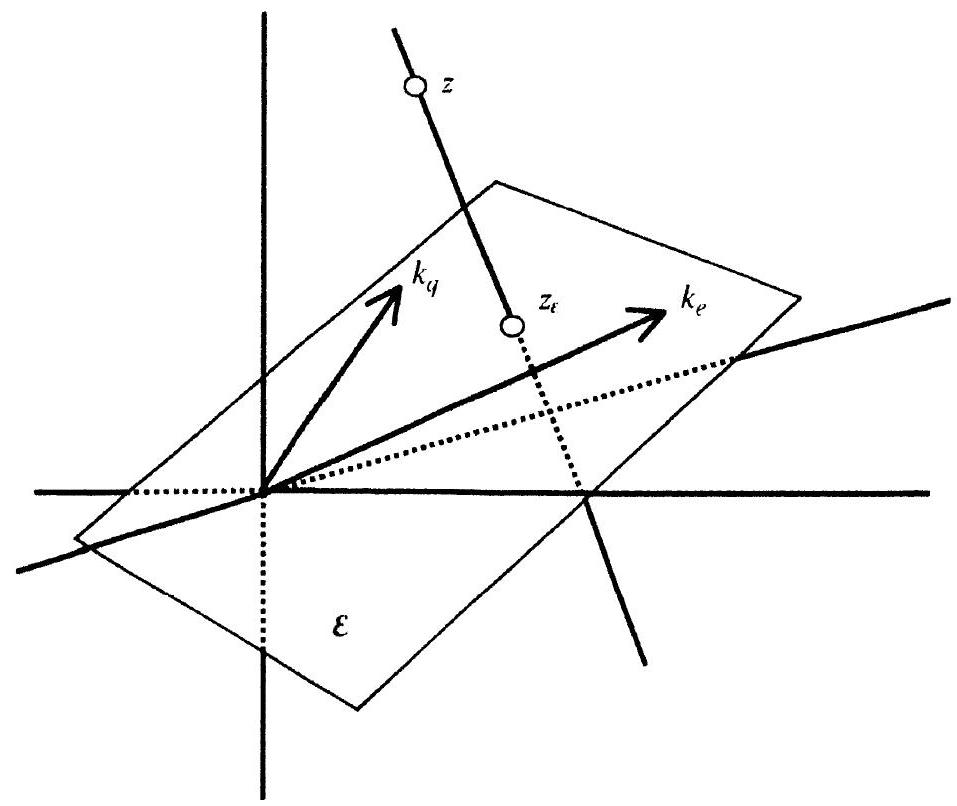
\includegraphics[max width=\textwidth]{2024_03_09_566eeb6d49daa183514ag-237}
% \end{center}

% Figure \ref{fig: 18.1} The set of frontier payoffs is the plane \(\mathcal{E}\) spanned by \(k_{q}\) and \(k_{e}\). Any payoff \(z\) can be projected onto \(\mathcal{E}\).

It follows from Theorem \ref{thm:mean_variance_frontier_characterization} that the return \(r_{q}\) on the pricing kernel and the return \(r_{e}\) on the expectations kernel are frontier returns. They are
\begin{equation*}
r_{e}=\frac{k_{e}}{E\left(k_{e} k_{q}\right)}=\frac{k_{e}}{E\left(k_{q}\right)} \quad \text { and } \quad r_{q}=\frac{k_{q}}{E\left(k_{q}^{2}\right)} 
\end{equation*}
where the pricing kernel was used to represent the prices of \(k_{q}\) and \(k_{e}\).

If the expectations kernel and the pricing kernel are collinear, then the returns \(r_{e}\) and \(r_{q}\) are the same. The set of frontier returns consists of the single return \(r_{e}\). If the risk-free payoff lies in the asset span, that single return equals the risk-free return \(\bar{r}\).

We assume throughout that the expectations kernel and the pricing kernel are not collinear. If \(k_{e}\) and \(k_{q}\) are not collinear, then the set of frontier returns is the line passing through the return \(r_{q}\) and the return \(r_{e}\). This line can be indexed by a single parameter \(\lambda\), and thus
\begin{equation*}
r_{\lambda}=r_{e}+\lambda\left(r_{q}-r_{e}\right), \label{eq:frontier_return_parametrization} 
\end{equation*}
where \(-\infty<\lambda<\infty\).

% \begin{center}
% 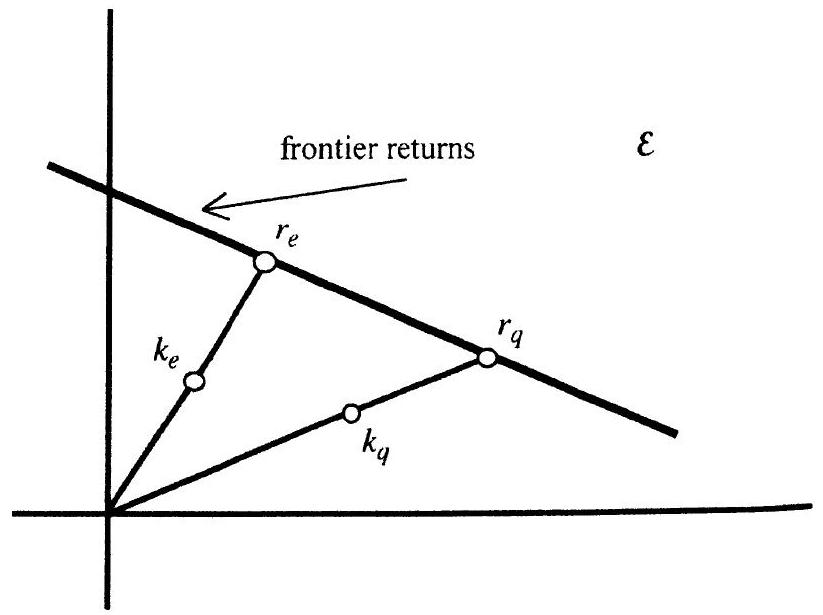
\includegraphics[max width=\textwidth]{2024_03_09_566eeb6d49daa183514ag-238}
% \end{center}

% Figure \ref{fig: 18.2} The frontier returns consist of the line connecting the return on the expectations kernel and the return on the pricing kernel.
\begin{example}\label{ex:mean_variance_frontier_example} Suppose that there are three equally likely states and that three securities are traded. The security returns are
\begin{gather*}
r_{1}=(3,0,0) \\
r_{2}=(0,6,0) \\
r_{3}=\left(\frac{6}{7}, \frac{3}{7}, \frac{9}{7}\right) . 
\end{gather*}
We wish to know which, if any, of these returns are on the mean-variance frontier.

To determine whether any of the security returns is a mean-variance frontier return, we locate the set of frontier returns. We first find the returns on the expectations and pricing kernels. Because markets are complete, the expectations kernel is the risk-free payoff $(1,1,1)$, and the pricing kernel is the state-price vector \(q\) rescaled by the probabilities of states. The state-price vector is the unique solution to the equations
\begin{gather*}
1=3 q_{1} \\
1=6 q_{2} \\
1=\frac{6}{7} q_{1}+\frac{3}{7} q_{2}+\frac{9}{7} q_{3} 
\end{gather*}
The solution is \(q_{1}=1 / 3, q_{2}=1 / 6, q_{3}=1 / 2\). The pricing kernel equals \(q / \pi\), that is $(1,1 / 2,3 / 2)$.
The returns of the expectations and pricing kernels are obtained using the pricing kernel. Because markets are complete the expectations kernel is $(1,1,1)$, and multiplying by the pricing kernel shows that its price is 1. Therefore its return \(r_{e}\) is $(1,1,1)$. The price of the pricing kernel $(1,1 / 2,3 / 2)$ is \(7 / 6\), and the return \(r_{q}\) equals \(r_{3}\). Return \(r_{3}\) is therefore a frontier return. Returns \(r_{1}\) and \(r_{2}\) are not, because they are not on the line connecting \(r_{e}\) and \(r_{q}\).
\end{example}
% \begin{center}
% 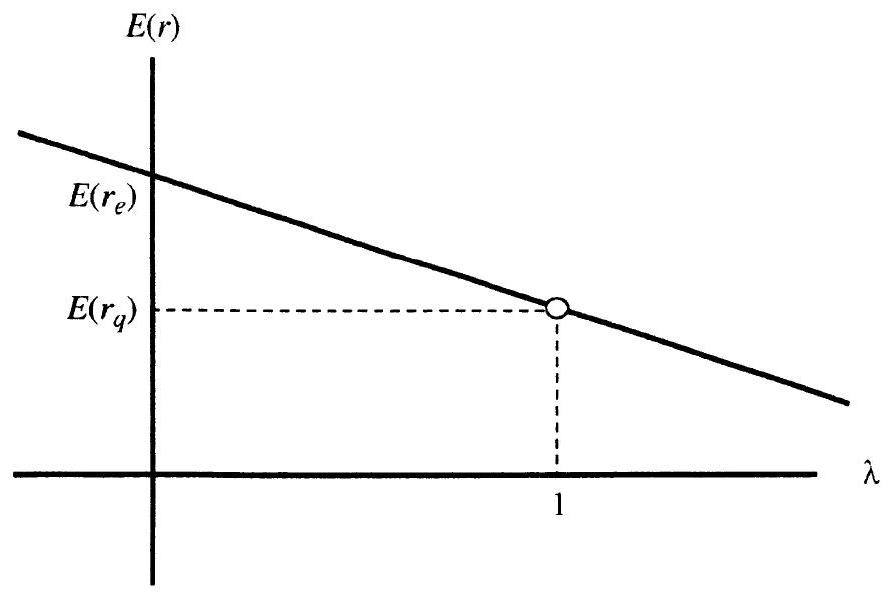
\includegraphics[max width=\textwidth]{2024_03_09_566eeb6d49daa183514ag-239(1)}
% \end{center}

% Figure \ref{fig: 18.3} Expected returns for frontier returns indexed by \(\lambda\). The expectations kernel has \(\lambda=0\), and the pricing kernel has \(\lambda=1\).
% The expectation of the frontier return \(r_{\lambda}\) defined by equation (\ref{18.3}) is
% \begin{equation*}
% E\left(r_{\lambda}\right)=E\left(r_{e}\right)+\lambda\left[E\left(r_{q}\right)-E\left(r_{e}\right)\right] . \label{18.10} 
% \end{equation*}
% The variance of \(r_{\lambda}\) is
% \begin{equation*}
% \operatorname{var}\left(r_{\lambda}\right)=\operatorname{var}\left(r_{e}\right)+2 \lambda \operatorname{cov}\left(r_{e}, r_{q}-r_{e}\right)+\lambda^{2} \operatorname{var}\left(r_{q}-r_{e}\right) \label{18.11} 
% \end{equation*}
% and its standard deviation \(\sigma\left(r_{\lambda}\right)\) is the square root of \(\operatorname{var}\left(r_{\lambda}\right)\). The expectations and standard deviations of frontier returns are shown in Figures 18.3-18.5.

% \begin{center}
% 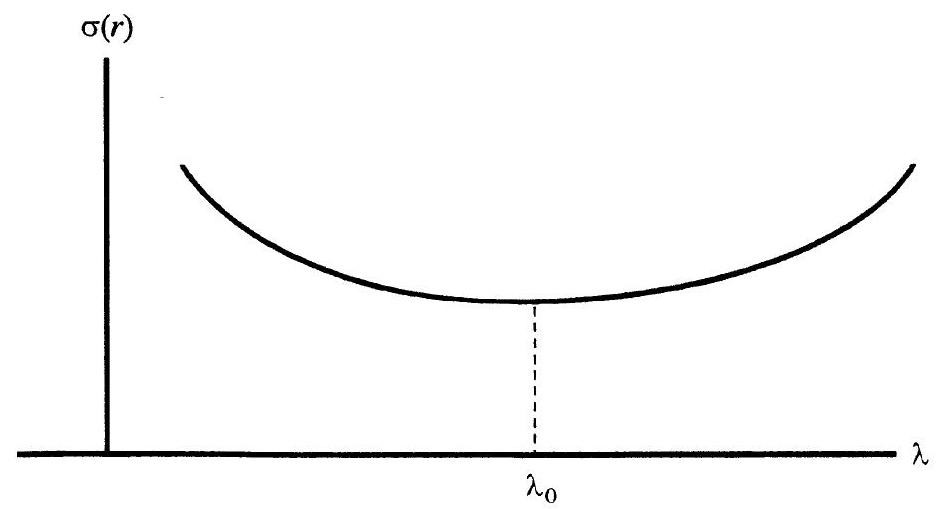
\includegraphics[max width=\textwidth]{2024_03_09_566eeb6d49daa183514ag-239}
% \end{center}

% Figure \ref{fig: 18.4} Standard deviation of frontier returns when there exists no risk-free return.

% \begin{center}
% 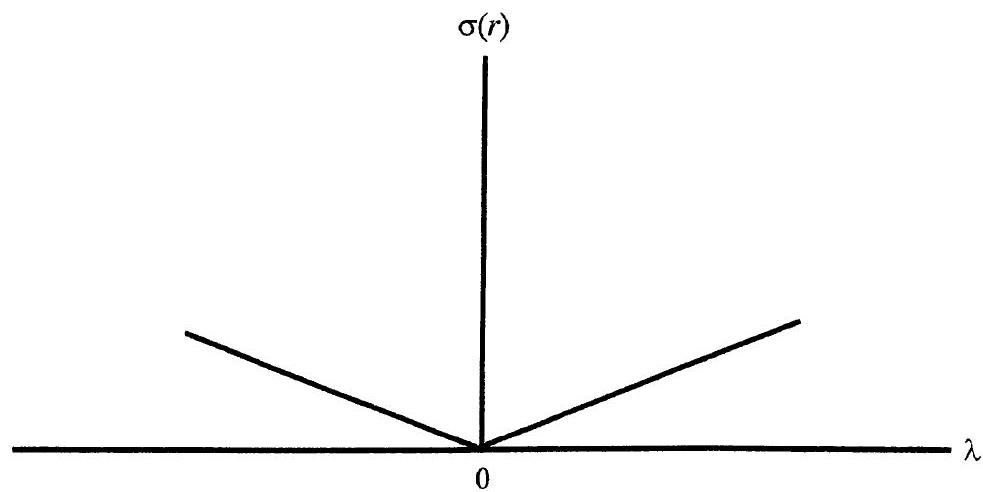
\includegraphics[max width=\textwidth]{2024_03_09_566eeb6d49daa183514ag-240}
% \end{center}

% Figure \ref{fig: 18.5} Standard deviation of frontier returns when there exists a risk-free return.

% \section*{Capital Asset Pricing Model}
% \subsection*{19.1 Introduction}
% Beta pricing (see Section 18.5) implies that the risk premium on any security or portfolio is proportional to the covariance of its return with a frontier return. However, beta pricing by itself gives no guidance as to which returns are frontier returns. We use the term "capital asset pricing model" (CAPM) if the market return is a frontier return. Note that the CAPM is here identified with a property of equilibrium security prices, not with a class of models of security markets (that is, the restriction involves endogenous variables, not exogenous variables). Therefore it is necessary to determine what restrictions on preferences or payoffs give rise to equilibria that conform to the CAPM definition.

% Under the CAPM the market return, being a frontier return, can be taken as the reference portfolio in the beta pricing equation. Doing so leads directly to the security market line, which relates the risk premium on any security to the covariance between the return on that security and the market return.

% In Chapter 14 we derived the equation of the security market line by applying consumption-based security pricing under the assumption that agents have quadratic utilities. The derivation was generalized in Chapter 16. In this chapter we derive the CAPM in an equilibrium under the assumption that agents take variance as a measure of consumption risk (mean-variance preferences). This condition is satisfied when agents' preferences have an expected utility representation with quadratic utilities (and also when security payoffs are multivariate normally distributed). We relax two of the assumptions of the Chapter 14 derivation: that agents' endowments lie in the asset span (security market economy) and that the risk-free payoff is in the asset span.

% \subsection*{19.2 Security Market Line}
% In Chapter 14 we defined the market payoff in a security market economy as the aggregate date-1 endowment \(\bar{w}_{1}\) and the market portfolio as a portfolio with payoff equal to the market payoff. We now extend these definitions to the general case in which agents' endowments, and therefore also the aggregate endowment, need not lie in the asset span.

% Each individual's date-1 endowment \(w_{1}^{i}\) can be decomposed into the sum of two orthogonal components. Using the expectations inner product, we project \(w_{1}^{i}\) onto the asset span to distinguish the tradable component of the aggregate endowment from a nontradable component that is orthogonal to the asset span. We have


% \begin{equation*}
% w_{1}^{i}=w_{1 \mathcal{M}}^{i}+w_{1 \mathcal{N}}^{i} \label{19.1} 
% \end{equation*}


% where \(w_{1 \mathcal{M}}^{i} \in \mathcal{M}\) is the tradable component of agent \(i\) 's endowment and \(w_{1 \mathcal{N}}^{i} \in\) \(\mathcal{N}=\mathcal{M}^{\perp}\) is the nontradable component. Theorem 17.5.1 (Projection Theorem) guarantees that there is no ambiguity about this decomposition. The corresponding decomposition for the aggregate endowment is


% \begin{equation*}
% \bar{w}_{1}=\bar{w}_{1 \mathcal{M}}+\bar{w}_{1 \mathcal{N}} \label{19.2} 
% \end{equation*}


% The market payoff \(m\) is defined as the tradable component of the aggregate endowment, that is,


% \begin{equation*}
% m=\bar{w}_{1 \mathcal{M}} \label{19.3} 
% \end{equation*}


% The market return \(r_{m}\) is the market payoff \(m\) divided by its equilibrium price \(q(m)\), which is assumed to be nonzero.

% By the definition of the CAPM, the market return \(r_{m}\) is a frontier return. If it is assumed that \(r_{m}\) is not the minimum-variance return, there exists another frontier return, denoted \(r_{m 0}\), that has zero covariance with \(r_{m}\). These two frontier returns can be used in equation (\ref{18.23}) of beta pricing. Thus, we have the following theorem.

% Theorem 19.2.1 (Security Market Line) If the market return lies on the meanvariance frontier, then


% \begin{equation*}
% E\left(r_{j}\right)=E\left(r_{m 0}\right)+\beta_{j}\left[E\left(r_{m}\right)-E\left(r_{m 0}\right)\right], \label{19.4} 
% \end{equation*}


% for every security \(j\), where \(\beta_{j}=\operatorname{cov}\left(r_{j}, r_{m}\right) / \operatorname{var}\left(r_{m}\right)\).

% Equation (\ref{19.4}) is the equation of the security market line. If the risk-free payoff is in the asset span, then \(r_{m 0}\) is risk free and equal to \(\bar{r}\), and equation (\ref{19.4}) becomes


% \begin{equation*}
% E\left(r_{j}\right)=\bar{r}+\beta_{j}\left[E\left(r_{m}\right)-\bar{r}\right] . \label{19.5} 
% \end{equation*}


% Equation (\ref{19.5}) says that the risk premium \(E\left(r_{j}\right)-\bar{r}\) is proportional to the coefficient \(\beta_{j}\), the factor of proportionality being the risk premium \(E\left(r_{m}\right)-\bar{r}\) on the market return (market risk premium). Thus coefficient \(\beta_{j}\) - the regression coefficient of \(r_{j}\) on the market return - is the appropriate measure of security risk in the CAPM.

% The equation of the security market line holds for portfolio returns as well. Substituting \(r\) and \(\beta\) for \(r_{j}\) and \(\beta_{j}\) in equation (\ref{19.4}), we obtain


% \begin{equation*}
% E(r)=E\left(r_{m 0}\right)+\beta\left[E\left(r_{m}\right)-E\left(r_{m 0}\right)\right], \label{19.6} 
% \end{equation*}


% where \(\beta\) is the regression coefficient of the return \(r\) on the market return. For the market return, \(\beta\) equals one; for the zero-covariance return \(r_{m 0}, \beta\) equals zero. Return \(r_{m 0}\) is called the zero-beta return.

% The following example illustrates the use of equation (\ref{19.5}) for pricing securities.

% Example 19.2.1 There are three equally probable states at date 1. The aggregate date-1 endowment is $(2,3,4)$. There are three securities: the first is risk free and has a return \(\bar{r}=1\); and the second has a return \(r_{2}=(0,3 / 2,3)\); and the third security has a payoff \(x_{3}=(0,0,1)\). The problem is to find the price \(p_{3}\) of the third security if the CAPM is assumed.

% We observe that the aggregate endowment lies in the span of the first and the second securities. This allows us to find the market return using the prices of those two securities. The price of the third security can be found using the security market line.

% The price of the market payoff is \(8 / 3\), and its return is \(r_{m}=(3 / 4,9 / 8,3 / 2)\). The expected return on the market portfolio is \(E\left(r_{m}\right)=9 / 8\).

% The security market line gives the following:


% \begin{equation*}
% \frac{E\left(x_{3}\right)}{p_{3}}=\bar{r}+\frac{\operatorname{cov}\left(x_{3}, r_{m}\right)}{p_{3} \operatorname{var}\left(r_{m}\right)}\left[E\left(r_{m}\right)-\bar{r}\right] \label{19.7} 
% \end{equation*}


% or


% \begin{equation*}
% p_{3}=\frac{1}{\bar{r}}\left(E\left(x_{3}\right)-\frac{\operatorname{cov}\left(x_{3}, r_{m}\right)}{\operatorname{var}\left(r_{m}\right)}\left[E\left(r_{m}\right)-\bar{r}\right]\right) . \label{19.8} 
% \end{equation*}


% Substituting \(E\left(r_{m}\right)=9 / 8, E\left(x_{3}\right)=1 / 3, \bar{r}=1, \operatorname{cov}\left(x_{3}, r_{m}\right)=1 / 8\), and \(\operatorname{var}\left(r_{m}\right)=\) \(3 / 32\) in equation (\ref{19.8}), we obtain \(p_{3}=1 / 6\).

% An alternative way of calculating \(p_{3}\) is to note that the pricing kernel lies in the frontier plane. Because the market payoff is in the frontier plane, the pricing kernel lies in the span of the market payoff and the risk-free payoff or, equivalently, in the span of \(r_{2}\) and the risk-free return. By writing the equations (\ref{17.31}) for pricing the risk-free return and \(r_{2}\), the pricing kernel can be calculated as $(3 / 2,1,1 / 2)$. Applying the kernel to \(x_{3}\) results in \(p_{3}=1 / 6\).

% The simplest case in which equation (\ref{19.5}) (the security market line) holds is when there are only two securities. We observed in Section 18.2 that with two securities every return is a mean-variance frontier return. In particular, the market return lies on the frontier and the CAPM holds.

% \subsection*{19.3 Mean-Variance Preferences}
% The CAPM obtains in equilibrium when agents have mean-variance preferences. An agent has mean-variance preferences if her utility function \(u\left(c_{0}, c_{1}\right)\) is strictly increasing and has the representation


% \begin{equation*}
% u\left(c_{0}, c_{1}\right)=v_{0}\left(c_{0}\right)+f\left[E\left(c_{1}\right), \operatorname{var}\left(c_{1}\right)\right] \label{19.9} 
% \end{equation*}


% for some functions \(v_{0}: \mathbb{R} \rightarrow \mathbb{R}\) and \(f: \mathbb{R} \times \mathbb{R}_{+} \rightarrow \mathbb{R}\). Under equation (\ref{19.9}), agents' preferences are time separable with preferences over date-1 consumption plans depending only on the expectation and variance. The agent therefore takes variance as a measure of consumption risk. An agent with mean-variance preferences is strictly variance averse if \(f\) in (\ref{19.9}) is strictly decreasing in variance.

% Two important cases that lead to mean-variance preferences - quadratic utilities and normally distributed payoffs and date-1 endowments - are discussed in Sections 19.5 and 19.6 .

% Theorem 19.3.1 If every agent has mean-variance preferences and is strictly variance averse, then in an equilibrium the market return lies on the mean-variance frontier.

% Proof: Let \(c_{1}^{i}\) be an equilibrium date-1 consumption plan of agent \(i\). We decompose \(c_{1}^{i}\) into the tradable component and the nontradable component (see equation (\ref{19.1})) so that


% \begin{equation*}
% c_{1}^{i}=c_{1 \mathcal{M}}^{i}+c_{1 \mathcal{N}}^{i}, \label{19.10} 
% \end{equation*}


% where \(c_{1 \mathcal{M}}^{i} \in \mathcal{M}\) and \(c_{1 \mathcal{N}}^{i} \in \mathcal{N}\).

% It is sufficient to show that the tradable component \(c_{1 \mathcal{M}}^{i}\) of each agent's date-1 consumption lies on the mean-variance frontier \(\mathcal{E}\) because if that is so, then the tradable component of the aggregate consumption is also a frontier payoff. But the tradable component of aggregate consumption equals the tradable component of the aggregate endowment, which by definition is the market payoff. Therefore, the market return is a frontier return.

% To show that \(c_{1 \mathcal{M}}^{i} \in \mathcal{E}\), we decompose \(c_{1 \mathcal{M}}^{i}\) by projecting it on the frontier plane \(\mathcal{E}\) so that


% \begin{equation*}
% c_{1 \mathcal{M}}^{i}=c_{1 \mathcal{E}}^{i}+c_{1 \mathcal{I}}^{i}, \label{19.11} 
% \end{equation*}


% where \(c_{1 \mathcal{E}}^{i} \in \mathcal{E}\) is the frontier component, and \(c_{1 \mathcal{I}}^{i} \in \mathcal{E}^{\perp}\) is the component of \(c_{1 \mathcal{M}}^{i}\) orthogonal to the frontier plane (here \(\mathcal{I}\) stands for "inefficient" and \(\mathcal{E}^{\perp}\) is the orthogonal complement of \(\mathcal{E}\) in \(\mathcal{M}\) ).

% Suppose by contradiction that, for some agent \(i, c_{1 \mathcal{M}}^{i}\) does not lie on the frontier plane and hence that \(c_{1 \mathcal{I}}^{i} \neq 0\). Consider the alternative date-1 consumption plan given by


% \begin{equation*}
% \tilde{c}_{1}^{i} := c_{1 \mathcal{E}}^{i}+c_{1 \mathcal{N}}^{i} \label{19.12} 
% \end{equation*}


% Note that \(\tilde{c}_{1}^{i}=c_{1}^{i}-c_{1 \mathcal{I}}^{i}\). Because the agent's utility function is strictly increasing, the optimal consumption satisfies the budget constraints with equality, implying that \(c_{1}^{i}-w_{1}^{i} \in \mathcal{M}\). If we use \(\tilde{c}_{1}^{i}-w_{1}^{i}=\left(c_{1}^{i}-w_{1}^{i}\right)-c_{1 \mathcal{I}}^{i}\), it follows that


% \begin{equation*}
% \tilde{c}_{1}^{i}-w_{1}^{i} \in \mathcal{M} \label{19.13} 
% \end{equation*}


% and thus the consumption plan \(\tilde{c}_{1}^{i}\) can be attained by a net trade in the asset span.

% By Theorem \ref{thm:mean_variance_frontier_characterization} the equilibrium pricing kernel \(k_{q}\) lies in the frontier plane \(\mathcal{E}\). Therefore,


% \begin{equation*}
% q\left(c_{1 \mathcal{I}}^{i}\right)=E\left(k_{q} c_{1 \mathcal{I}}^{i}\right)=0 \label{19.14} 
% \end{equation*}


% and the net trade \(\tilde{c}_{1}^{i}-w_{1}^{i}\) has the same price as \(c_{1}^{i}-w_{1}^{i}\); that is, \(q\left(\tilde{c}_{1}^{i}-w_{1}^{i}\right)=\) \(q\left(c_{1}^{i}-w_{1}^{i}\right)\). This and equation (\ref{19.13}) imply that the date-1 consumption plan \(\tilde{c}_{1}^{i}\) and the date-0 plan \(c_{0}^{i}\) satisfy agent \(i\) 's budget constraint.

% Because the expectations kernel also lies in the frontier plane (Theorem \ref{thm:mean_variance_frontier_characterization}), we have


% \begin{equation*}
% E\left(c_{1 \mathcal{I}}^{i}\right)=E\left(k_{e} c_{1 \mathcal{I}}^{i}\right)=0 \label{19.15} 
% \end{equation*}


% Therefore, \(\tilde{c}_{1}^{i}\) and \(c_{1}^{i}\) have the same expectation. Because \(c_{1 \mathcal{E}}^{i}, c_{1 \mathcal{I}}^{i}\), and \(c_{1 \mathcal{N}}^{i}\) are mutually orthogonal and \(E\left(c_{1 \mathcal{I}}^{i}\right)=0\), it follows that \(\operatorname{cov}\left(c_{1 \mathcal{E}}^{i}, c_{1 \mathcal{I}}^{i}\right)=\operatorname{cov}\left(c_{1 \mathcal{I}}^{i}, c_{1 \mathcal{N}}^{i}\right)=0\). Using equation (\ref{19.12}), we obtain that \(\operatorname{cov}\left(\tilde{c}_{1}^{i}, c_{1 \mathcal{I}}^{i}\right)=0\) and consequently that


% \begin{equation*}
% \operatorname{var}\left(c_{1}^{i}\right)=\operatorname{var}\left(\tilde{c}_{1}^{i}\right)+\operatorname{var}\left(c_{1 \mathcal{I}}^{i}\right)>\operatorname{var}\left(\tilde{c}_{1}^{i}\right), \label{19.16} 
% \end{equation*}


% where the last strict inequality follows from the assumption that \(c_{1 \mathcal{I}}^{i} \neq 0\).

% Consumption plan \(\tilde{c}_{1}^{i}\) has lower variance than \(c_{1}^{i}\), and the two have the same expectation. Because the agent has mean-variance preferences and is strictly variance averse, consumption plan \(\tilde{c}_{1}^{i}\) is strictly preferred to \(c_{1}^{i}\). This contradicts the optimality of \(c_{1}^{i}\). Therefore, the tradable component \(c_{1 \mathcal{M}}^{i}\) of every agent's equilibrium consumption lies in the mean-variance frontier plane. Because in equilibrium the market payoff equals the sum over agents of the tradable components of\\
% agents' consumption plans, the market return lies on the mean-variance frontier as well.

% It follows from Theorems 19.2.1 and 19.3.1 that if agents measure consumption risk by variance, then beta, the coefficient of regression of the return on the market return, is the appropriate measure of security risk in equilibrium.

% \subsection*{19.4 Equilibrium Portfolios under Mean-Variance Preferences}
% In the proof of Theorem 19.3.1 we demonstrated that the tradable component of the date-1 equilibrium consumption plan of an agent with mean-variance preferences lies on the mean-variance frontier. The nontradable component of the equilibrium consumption plan is equal to the nontradable component of the endowment. To see this, note that because \(c_{1}^{i}-w_{1}^{i} \in \mathcal{M}\), equations (\ref{19.1}) and (\ref{19.10}) imply that


% \begin{equation*}
% c_{1 \mathcal{N}}^{i}=w_{1 \mathcal{N}}^{i} \label{19.17} 
% \end{equation*}


% If the risk-free payoff lies in the asset span, then \(c_{1 \mathcal{N}}^{i}\) has zero expectation because it is orthogonal to the asset span. If not, \(c_{1 \mathcal{N}}^{i}\) does not have zero expectation. Summing up, the equilibrium date-1 consumption plan satisfies


% \begin{equation*}
% c_{1}^{i}=c_{1 \mathcal{M}}^{i}+w_{1 \mathcal{N}}^{i}, \quad \text { with } \quad c_{1 \mathcal{M}}^{i} \in \mathcal{E} . \label{19.18} 
% \end{equation*}


% Let


% \begin{equation*}
% w^{i} := w_{0}^{i}+q\left(w_{1 \mathcal{M}}^{i}\right) \label{19.19} 
% \end{equation*}


% be the agent's wealth at date 0 consisting of his date-0 endowment and the value of the tradable component of his date-1 endowment. Because the mean-variance frontier is spanned by the market return \(r_{m}\) and the zero-covariance return \(r_{m 0}\), the tradable component of date-1 equilibrium consumption plan can be written as


% \begin{equation*}
% c_{1 \mathcal{M}}^{i}=a^{i} r_{m}+\left(w^{i}-c_{0}^{i}-a^{i}\right) r_{m 0}, \label{19.20} 
% \end{equation*}


% where \(a^{i}\) denotes the amount of date-0 wealth invested in the market portfolio. A simple characterization of the equilibrium investment \(a^{i}\) can be given when the risk-free payoff lies in the asset span. Then \(r_{m 0}=\bar{r}\) and the expectation and variance of date-1 equilibrium consumption plan can be written using equations (\ref{19.18}) and (\ref{19.20}) as


% \begin{equation*}
% E\left(c_{1}^{i}\right)=\left(w^{i}-c_{0}^{i}\right) \bar{r}+a^{i}\left[E\left(r_{m}\right)-\bar{r}\right], \label{19.21} 
% \end{equation*}


% and


% \begin{equation*}
% \operatorname{var}\left(c_{1}^{i}\right)=\left(a^{i}\right)^{2} \operatorname{var}\left(r_{m}\right)+\operatorname{var}\left(w_{1 \mathcal{N}}^{i}\right) . \label{19.22} 
% \end{equation*}


% The equilibrium investment \(a^{i}\) and consumption plan \(c^{i}\) (assumed interior and with strictly positive variance) satisfy the following first-order conditions obtained from substituting equations (\ref{19.21}) and (\ref{19.22}) in equation (\ref{19.9}) and maximizing with respect to \(c_{0}^{i}\) and \(a^{i}\) :
% \begin{align}
% v_{0}^{\prime} & =\bar{r} \partial_{E} f  \label{19.23} \\
% a^{i} & =-\frac{\left(E\left(r_{m}\right)-\bar{r}\right) \partial_{E} f}{2 \operatorname{var}\left(r_{m}\right) \partial_{v} f} \label{19.24} 
% \end{align}
% Here \(\partial_{E} f\) and \(\partial_{v} f\) are the partial derivatives of \(f\) with respect to its first and second arguments evaluated at the equilibrium date-1 consumption; \(v_{0}^{\prime}\) is the derivative of \(v_{0}\) evaluated at the equilibrium date-0 consumption.

% Equation (\ref{19.23}) states that the marginal rate of substitution between date-0 consumption and the expectation of date-1 consumption equals the risk-free return. Equation (\ref{19.24}) relates the equilibrium investment in the market portfolio to the risk premium and the variance of the market return, and also to the marginal rate of substitution between expected return and variance of return.

% If each agent's mean-variance utility function is strictly increasing in the expectation of date-1 consumption and strictly decreasing in its variance, then all agents whose optimal consumption is not risk-free have investments in the market portfolio that are of the same sign as the risk premium on the market return. It follows that the market risk premium must be strictly positive because otherwise the total wealth invested in the market portfolio would be negative. Thus


% \begin{equation*}
% E\left(r_{m}\right)>\bar{r} \label{19.25} 
% \end{equation*}


% Consequently, each agent's investment in the market portfolio is strictly positive or zero, implying that the expected return on equilibrium investment exceeds the risk-free return. Because every mean-variance frontier return with expectation that exceeds the risk-free return is mean-variance efficient, returns on agents' equilibrium investments are mean-variance efficient.

% The foregoing discussion provides a characterization of an equilibrium portfolio net of the portfolio that generates the tradable component of an agent's date-1 endowment. The agent's equilibrium portfolio is equal to the difference between the portfolio described earlier and the portfolio that generates \(w_{1 \mathcal{M}}^{i}\).

% \subsection*{19.5 Quadratic Utilities}
% If an agent's preferences have an expected utility representation with a quadratic utility function of the form


% \begin{equation*}
% v^{i}\left(c_{0}, c_{s}\right)=v_{0}^{i}\left(c_{0}\right)+v_{1}^{i}\left(c_{s}\right)=v_{0}^{i}\left(c_{0}\right)-\left(c_{s}-\alpha^{i}\right)^{2}, \quad \text { for } \quad c_{s} \leq \alpha^{i}, \label{19.26} 
% \end{equation*}


% then the expected utility of consumption \(\left(c_{0}, c_{1}\right)\) is


% \begin{equation*}
% E\left[v^{i}\left(c_{0}, c_{1}\right)\right]=v_{0}^{i}\left(c_{0}\right)-\left\{\operatorname{var}\left(c_{1}\right)+\left[E\left(c_{1}\right)-\alpha^{i}\right]^{2}\right\} \label{19.27} 
% \end{equation*}


% As usual, we assume common probability expectations. The agent's expected utility (equation (\ref{19.27})) depends only on \(c_{0}\) and the expectation and variance of \(c_{1}\). Thus, the agent has mean-variance preferences and is strictly variance averse. Theorem 19.3.1 therefore applies when utility functions are quadratic.

% In Chapter 14, with the subsequent generalization in Chapter 16, we derived the equation of the security market line in an equilibrium with quadratic utility functions (\ref{19.26}) under additional assumptions not appearing in Theorem 19.3.1: that agents' endowments lie in the asset span and that the risk-free payoff is in the asset span. Further, we proved in Chapter 16 that under these assumptions, markets are effectively complete and equilibrium consumption allocations are Pareto optimal. From the analysis of this chapter we conclude that the equation of the security market line holds in an equilibrium with quadratic utility functions even when either agents' endowments or the risk-free payoff or both lie outside of the asset span. However, the Pareto optimality of equilibrium consumption allocations does not in general hold under the less strict assumptions.

% \subsection*{19.6 Normally Distributed Payoffs}
% If security payoffs and an agent's date-1 endowment are multivariate normally distributed, \({ }^{1}\) then her date-1 consumption plans that can be generated by portfolios are normally distributed. Because the normal distribution is completely characterized by its expectation and variance, the agent's utility function depends only on date-0 consumption \(c_{0}\) and the expectation and variance of date-1 consumption plan \(c_{1}\). If her utility functions are time separable and strictly increasing, the agent has mean-variance preferences 19.9 .

% In particular, if an agent's preferences have an expected utility representation with a time-separable utility function, the mean-variance representation obtains when security payoffs and his date-1 endowment are multivariate normally distributed. Further, if the agent is risk averse, then he is also variance averse. To see this, recall from Section 10.3 that if two random variables are normally distributed, then the one with strictly greater variance is strictly riskier. Thus Theorem 19.3.1 applies when security payoffs and agents' date-1 endowments are multivariate normally distributed and agents are risk averse.
% \footnotetext{1 Strictly, normal distribution of payoffs cannot be incorporated in the model adopted in this book because we assumed that there exists only a finite number of states. However, no harm results if we temporarily trespass into a richer setting.
% }

% Normal payoff distributions can be justified by appeal to the central limit theorem. But that is only if security payoffs are not subject to limited liability. For instance, the payoff of an option is a truncated version of the payoff on the underlying security.

% \subsection*{19.7 Notes}
% A first expression of the risk-return tradeoff was given in Theorem 13.2.1. In a world of risk-averse investors, the greater the expected return on an optimal portfolio, the greater the risk. We observed in Chapter 10 that even if no assumptions about the form of the utility function are made (other than risk aversion), a specific measure of return was available: expected return. We also remarked that in general variance cannot be used as a measure of risk. Instead, risk must be associated with the partial ordering defined in Chapter 10. In the CAPM, in contrast, risk is associated with the complete ordering of return distributions induced by beta, and the security market line implies that the relation between expected return and risk is linear.

% If the risk-free payoff and agents' endowments lie in the asset span, the CAPM shares with LRT utilities a property of equilibrium: that date-1 consumption plans lie in the plane spanned by the aggregate endowment and the risk-free payoff. However, the pricing relationship of the CAPM - the security market line - does not apply in the general LRT utilities case (with the exception, of course, of quadratic utilities). Nothing about the assumption that agents have LRT utilities with a common slope of risk tolerance implies that the market payoff is mean-variance efficient. As was shown in Theorem 19.3.1, mean-variance efficiency of the market payoff is a consequence of the assumption that agents measure consumption risk by variance. In proving Theorem 19.3.1, we assumed that agents' consumption plans were unrestricted. If there are restrictions on consumption (such as positivity), the theorem is still true provided that the equilibrium allocation is interior. But the proof requires a minor modification. Instead of using \(\tilde{c}_{1}^{i}=c_{1}^{i}-c_{1 \mathcal{I}}^{i}\) as an alternative consumption plan, it is necessary to use \(\tilde{c}_{1}^{i}=c_{1}^{i}-\delta c_{1 \mathcal{L}}^{i}\) for small positive \(\delta\). Although the first of these consumption plans may not be in the consumption set even if \(c_{1}^{i}\) is interior, the latter will be for small enough \(\delta\).

% The portfolio theory under mean-variance preferences originated with Markowitz [3]. The CAPM pricing results were derived independently by Sharpe [10], Lintner, [2], Mossin [5], and Treynor [11].

% Derivation of the CAPM without the assumption that the risk-free payoff is traded is from Black [1]. Sufficient conditions for the existence of a CAPM equilibrium when agents have mean-variance preferences, with and without a risk-free security, can be found in Nielsen [6] and [7].

% The testable content of the CAPM is the assertion that the market return is mean-variance efficient, which implies the equation of the security market line. In his critique, Roll [8] observed that if one uses a proxy for the market portfolio that is not mean-variance efficient, testing the relation between beta and risk premia is pointless. That is because the CAPM generates a prediction about this relation only when the reference portfolio is mean-variance efficient.

% As noted by Ross [9], if the proxy for the market portfolio is mean-variance efficient, the equation of the security market line will be satisfied regardless of whether the CAPM is true. This we showed in Chapter 18.

% Milne and Smith [4] analyzed the CAPM in the presence of transaction costs.

% \section*{Bibliography}
% [1] Fischer Black. Capital market equilibrium with restricted borrowing. Journal of Business, 45:444-455, 1972.

% [2] John Lintner. The valuation of risk assets and the selection of risky investments in stock portfolios and capital budgets. Review of Economics and Statistics, 47:13-37, 1965.

% [3] Harry Markowitz. Portfolio Selection: Efficient Diversification of Investments. Wiley, New York, 1959.

% [4] Frank Milne and Clifford W. Smith. Capital asset pricing with proportional transaction cost. Journal of Financial and Quantitative Analysis, XV:253-266, 1980.

% [5] Jan Mossin. Equilibrium in a capital asset market. Econometrica, 35:768-783, 1968.

% [6] Lars T. Neilsen. Equilibrium in CAPM without a riskless asset. Review of Economic Studies, 57:315-324, 1990.

% [7] Lars T. Neilsen. Existence of equilibrium in CAPM. Journal of Economic Theory, 52:223-231, 1990.

% [8] Richard Roll. A critique of the asset pricing theory's tests: Part I. Journal of Financial Economics, 4:129-176, 1977.

% [9] Stephen A. Ross. Risk, return and arbitrage. In Irwin Friend and James Bicksler, editors, Risk and Return in Finance. Ballinger, Cambridge, MA, 1976.

% [10] William F. Sharpe. Capital asset prices: A theory of market equilibrium under conditions of risk. Journal of Finance, 19:425-442, 1964.

% [11] John L. Treynor. Toward a theory of market value of risky assets. Mimeo. 1961.



% \section*{Equilibrium in Multidate Security Markets}
% \subsection*{21.1 Introduction}
% We have thus far limited ourselves to models of two-date security markets in which securities are traded only once before their payoffs are realized. These models are suitable for the introductory study of the risk-return relation for securities and the role of securities in the equilibrium allocation of risk. However, two-date models require the assumption that all uncertainty is resolved at once. It is more realistic to assume that uncertainty is resolved only gradually. As the uncertainty is resolved, agents trade securities again and again. The multidate model of this and the following chapters assumes that there are a finite number of future dates. This specification allows for the gradual resolution of uncertainty and the retrading of securities as new information about security prices and payoffs becomes available.

% \subsection*{21.2 Uncertainty and Information}
% In the multidate model, just as in the two-date model, uncertainty is specified by a set of states \(S\). Each of the states is a description of the economic environment for all dates \(t=0,1, \ldots, T\). At date 0 agents do not know which state will be realized. But as time passes, they obtain more and more information about the state. At date \(T\) they learn the actual state.

% Formally, the information of agents at date \(t\) is described by a partition \(F_{t}\) of the set of states \(S\) (a partition \(F_{t}\) of \(S\) is a collection of subsets of \(S\) such that each state \(s\) belongs to exactly one element of \(F_{t}\) ). The interpretation is that at date \(t\) agents know the element of the date- \(t\) partition to which the actual state belongs. They do not know which state of the known element of the date- \(t\) partition is the actual state, but they do know that states that do not belong to that element cannot be realized. The partitions are assumed to be common across agents; that is, all agents have the same information.

% \begin{center}
% 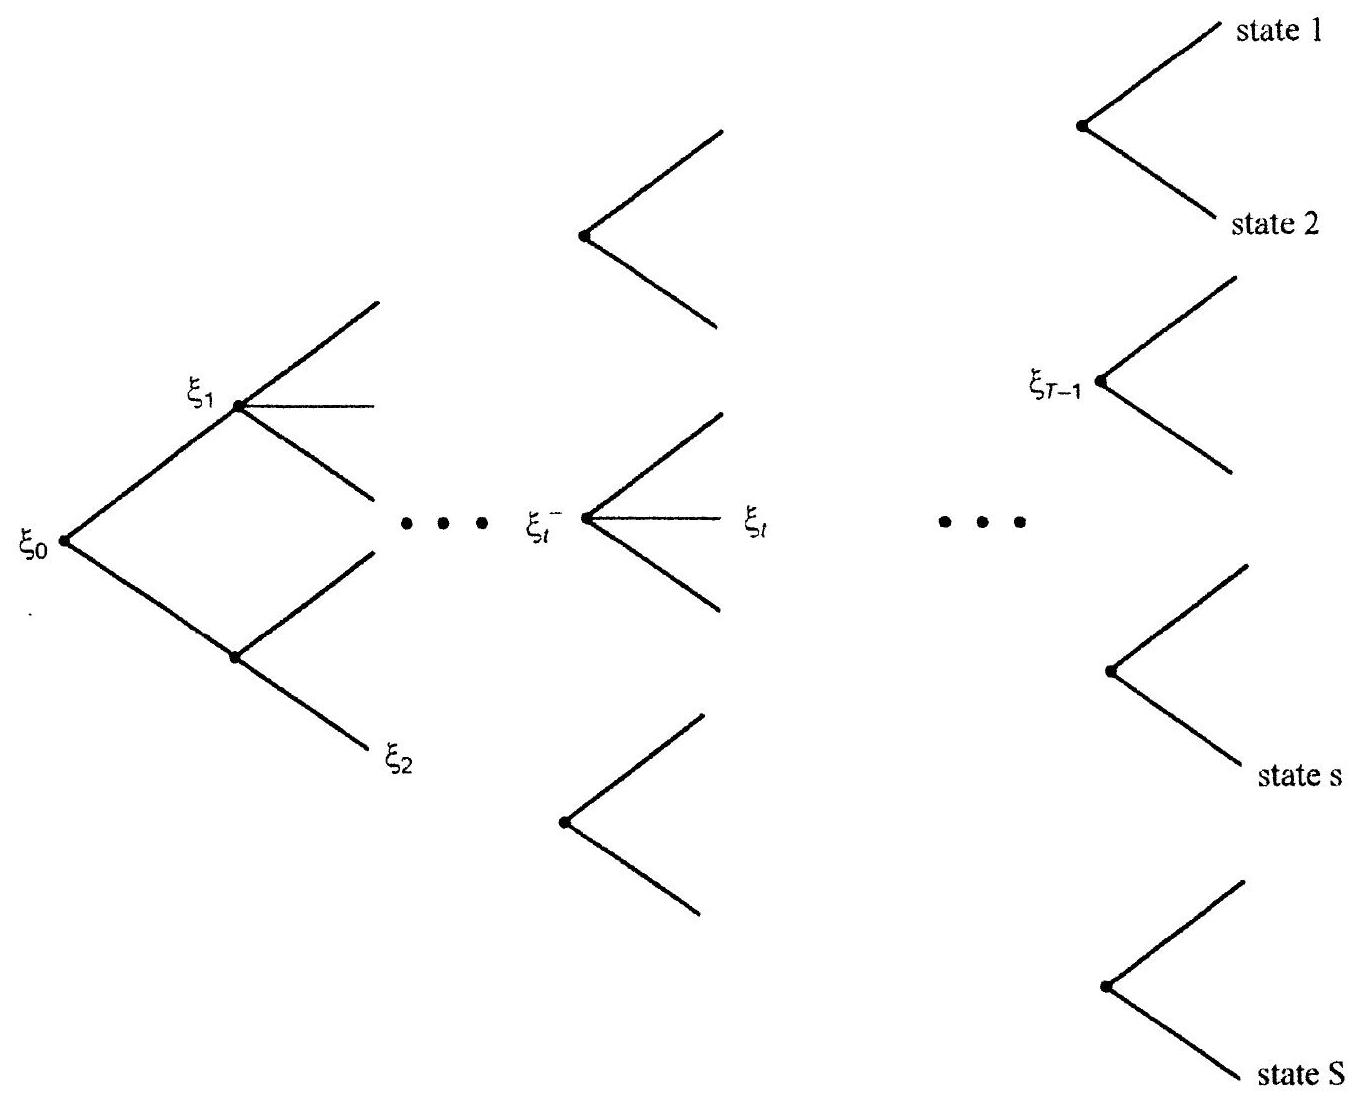
\includegraphics[width=\textwidth]{2024_03_09_566eeb6d49daa183514ag-274}
% \end{center}

% Figure \ref{fig: 21.1} An event tree. The initial node is indicated by \(\xi_{0}\). The nodes at the terminal date coincide with the states. Generic nodes at dates \(1, t\), and \(T-1\) are indicated by \(\xi_{1}, \xi_{t}\), and \(\xi_{T-1}\), respectively. The precedecessor node to \(\xi_{t}\) is indicated by \(\xi_{t}^{-}\).

% At date 0 agents have no information about the state, and thus the date-0 partition is the trivial partition \(F_{0}=\{S\}\). At date \(T\), agents have full information, and therefore the date- \(T\) partition is the total partition \(F_{T}=\{\{s\}: s \in S\}\). At dates \(1, \ldots, T-1\), agents have intermediate amounts of information. The partition \(F_{t+1}\) is finer (but not necessarily strictly finer) than partition \(F_{i}\); that is, the element of date- $(t+1)$ partition to which a state belongs is a subset of the element of date- \(t\) partition to which it belongs. Equivalently, if two states belong to different elements of the date- \(t\) partition, they cannot belong to the same element of the partition at any date after \(t\). Thus, agents never forget anything they once knew; their information about the state is nondecreasing. The $(T+1)$-tuple of partitions \(\left\{F_{0}, F_{1}, \ldots, F_{T}\right\}\) is the information filtration \(\mathcal{F}\).

% Another term for an information filtration (in the finite case studied here) is an event tree (figure \ref{fig: 21.1}). Each element of partition \(F_{t}\) is called a date-t event and is a node of the event tree. The event \(\xi_{0}=F_{0}\) is the root node. The successors of the event \(\xi_{t}\) are the events \(\xi_{\tau} \subset \xi_{t}\) for \(\tau>t\). The immediate successors of \(\xi_{t}\) are\\
% the events \(\xi_{t+1} \subset \xi_{t}\). The predecessors of \(\xi_{t}\) are the events \(\xi_{\tau} \supset \xi_{t}\), for \(\tau<t\). The unique immediate predecessor of \(\xi_{t}\) is the event \(\xi_{t-1}\) such that \(\xi_{t-1} \supset \xi_{t}\). Sometimes the immediate predecessor of \(\xi_{t}\) is denoted \(\xi_{t}^{-}\).

% The set of all events at all future dates \(t=1, \ldots, T\) is denoted \(\Xi\), and \(k=\#(\Xi)\) is the number of events in \(\Xi\). The number of events including \(\xi_{0}\) is thus \(k+1\).

% Example 21.2.1 Suppose that the only relevant information is profit reports of two firms. Each of the reports is either good (G) or bad (B). One firm issues its report at date 1 , the other at date 2 . The set of states \(S\) consists of the four possible outcomes of the two reports: \(\{\mathrm{GG}, \mathrm{GB}, \mathrm{BG}, \mathrm{BB}\}\). The information filtration is


% \begin{align}
% & F_{0}=\{\{\mathrm{GG}, \mathrm{GB}, \mathrm{BG}, \mathrm{BB}\}\},  \label{21.1} \\
% & F_{1}=\{\{\mathrm{GG}, \mathrm{GB}\},\{\mathrm{BG}, \mathrm{BB}\}\},  \label{21.2} \\
% & F_{2}=\{\{\mathrm{GG}\},\{\mathrm{GB}\},\{\mathrm{BG}\},\{\mathrm{BB}\}\} . \label{21.3} 
% \end{align}
% Thus at date 0 agents know nothing, at date 1 they know the profit report of the first firm, and at date 2 they know the profit reports of both firms.

% Because this example will come up again, it is convenient to introduce a compact notation for events. Thus, we let
% \begin{equation*}
% \xi_{\mathrm{g}} :=\{\mathrm{GG}, \mathrm{GB}\}, \quad \xi_{\mathrm{b}} :=\{\mathrm{BG}, \mathrm{BB}\} \label{21.4} 
% \end{equation*}
% be the two date-1 events and
% \begin{equation*}
% \xi_{\mathrm{gg}} :=\{\mathrm{GG}\}, \quad \xi_{\mathrm{gb}} :=\{\mathrm{GB}\}, \quad \xi_{\mathrm{bg}} :=\{\mathrm{BG}\}, \quad \xi_{\mathrm{bb}} :=\{\mathrm{BB}\} \label{21.5} 
% \end{equation*}

% be the four date- 2 events. The set of all future events is \(\Xi=\left\{\xi_{\mathrm{g}}, \xi_{\mathrm{b}}, \xi_{\mathrm{gg}}, \xi_{\mathrm{gb}}\right.\), \(\left.\xi_{\mathrm{bg}}, \xi_{\mathrm{bb}}\right\}\).

% Agents' information about the state has to be reflected properly in all economic variables such as endowments, security prices and dividends, portfolio holdings, consumption plans, and so forth. Specifically, it would not make sense to consider consumption plans or security prices at date \(t\) that differ in states that cannot be distinguished based on the information available to agents at date \(t\). One way to specify these variables is to represent them as functions on the set of states \(S\) and require that they be measurable with respect to the partition \(F_{t}\). If consumption at date \(t\) is represented by a function \(c_{t}: S \rightarrow \mathbb{R}\) that takes value \(c_{t}(s)\) in state \(s\), then measurability of \(c_{t}\) with respect to partition \(F_{t}\) requires that \(c_{t}(s)=c_{t}\left(s^{\prime}\right)\) for each \(s\) and \(s^{\prime}\) that belong to a common element \(\xi_{t}\) of \(F_{t}\).

% The measurability requirement can be embedded in the notation by using events rather than states to distinguish different values of functions. If \(c_{t}\) is measurable\\
% with respect to \(F_{t}\), then, by definition, \(c_{t}(s)=c_{t}\left(s^{\prime}\right)\) for all \(s, s^{\prime}\) in a given date- \(t\) event \(\xi_{t}\), and we can denote this common value by \(c\left(\xi_{t}\right){ }^{1}\)

% At times we use \(c_{t}\) to denote the vector (of dimension equal to the number of events at date \(t\) ) of values \(c\left(\xi_{t}\right)\) for all \(\xi_{t} \in F_{t}\). Thus we use the same notation \(c_{t}\) for the consumption plan as an \(F_{t}\)-measurable function on the set of states and as a vector with dimension equal to the number of events at \(t\). The distinction often does not matter; when it does, the intended meaning will always be clear from the context. Similarly, we use \(c\) to denote either a $(T+1)$-tuple of \(F_{t}\)-measurable functions \(c_{t}\) or a $(k+1)$-dimensional vector of values \(c(\xi)\) for all \(\xi \in \Xi\).

% If every function \(c_{t}\) in the $(T+1)$-tuple \(c\) is \(F_{t}\)-measurable, then \(c\) is adapted to the information filtration \(\mathcal{F}\).

% \subsection*{21.3 Multidate Security Markets}
% There exist \(J\) securities. Each security is characterized by the dividends it pays at each date. By the dividend we mean any payment to which a security holder is entitled. For stocks, dividends are firms' profit distributions to stockholders; for bonds, dividends are coupon payments and payments at maturity.

% The dividend on security \(j\) in event \(\xi_{t}\) is denoted by \(x_{j}\left(\xi_{t}\right)\). We use \(x_{j t}\) in place of \(x_{j}\left(\xi_{t}\right)\) when it is not necessary to indicate the event explicitly, \(x_{t}\) to denote the vector of dividends on all \(J\) securities in all date- \(t\) events, and \(x\) to denote dividends on all securities at all dates.

% There are no dividends at date 0 . It is possible that a security has a nonzero dividend only at a single date. For instance, a zero-coupon bond that matures at date \(t\) with face value 1 has dividends equal to 1 in each date- \(t\) event and zero dividends at all other dates.

% Securities are traded at all dates except the terminal date \(T\). Security prices are ex-dividend, meaning that the dividend on a security that is transferred at event \(\xi_{t}\) goes to the seller, not the buyer. The price of security \(j\) in event \(\xi_{t}\) is denoted by \(p_{j}\left(\xi_{t}\right)\). For notational convenience we have date- \(T\) prices \(p_{j}\left(\xi_{T}\right)\) even though trade does not take place at date \(T\). These prices are all set equal to zero. We use \(p_{j t}\) to denote the vector of prices \(p_{j}\left(\xi_{t}\right)\) in all date- \(t\) events \(\xi_{t}\), and \(p_{t}\) to denote the vector of prices of all \(J\) securities in all date-t events. One can take the dimension of \(p_{j t}\) to equal either the number of states or the number of events at date \(t\), as a matter of convenience.

% The holding of security \(j\) in event \(\xi_{t}\) is denoted by \(h_{j}\left(\xi_{t}\right)\) or \(h_{j t}\), and the portfolio of \(J\) securities in event \(\xi_{t}\) is denoted by \(h\left(\xi_{t}\right)\) or \(h_{t}\). The holding of each security may be positive, zero, or (unless a short-sale constraint has been imposed) negative.
% \footnotetext{\({ }^{1}\) Note that we write \(c\left(\xi_{t}\right)\) instead of \(c_{t}\left(\xi_{t}\right)\) to simplify notation.
% }

% We have, again for notational convenience, a date- \(T\) portfolio \(h\left(\xi_{T}\right)\), which is set equal to zero. The $(T+1)$-tuple \(h=\left(h_{0}, \ldots, h_{T}\right)\) is a portfolio strategy.

% The gross payoff of a portfolio strategy \(h\) in event \(\xi_{t}\) is the dividends on the portfolio chosen in the immediate predecessor node \(\xi_{t}^{-}\)plus the value at prices prevailing at \(\xi_{t}\) of the securities chosen at the predecessor node: \(\left(p\left(\xi_{t}\right)+x\left(\xi_{t}\right)\right) h\left(\xi_{t}^{-}\right)\). The payoff of a portfolio strategy \(h\), denoted by \(z(h, p)\left(\xi_{t}\right)\), equals the gross payoff minus the cost of the portfolio chosen at \(\xi_{t}\) :


% \begin{equation*}
% z(h, p)\left(\xi_{t}\right) :=\left(p\left(\xi_{t}\right)+x\left(\xi_{t}\right)\right) h\left(\xi_{t}^{-}\right)-p\left(\xi_{t}\right) h\left(\xi_{t}\right) \label{21.6} 
% \end{equation*}


% Thus the payoff equals the magnitude of the payment at \(\xi_{t}\) to the investor (or, if negative, from the investor). We use \(z_{t}(h, p)\) to denote the vector of payoffs \(z(h, p)\left(\xi_{t}\right)\) in all date- \(t\) events \(\xi_{t}\). The price at date 0 of a portfolio strategy \(h\) is \(p\left(\xi_{0}\right) h\left(\xi_{0}\right)\). If payoffs of a portfolio strategy are zero in every event at every date other than the initial and terminal dates, the portfolio strategy is termed a self-financing portfolio strategy.

% We present two examples of portfolio strategies and their payoffs.

% Example 21.3.1 Consider the portfolio strategy that involves buying one share of security \(j\) in event \(\xi_{t}\) at date \(t \geq 1\) and selling it in every immediate successor event of \(\xi_{t}\). This portfolio strategy is represented by the vector \(h\), which has 1 in the position associated with the holding of security \(j\) in event \(\xi_{t}\) and zeros elsewhere. Its payoff equals \(-p_{j}\left(\xi_{t}\right)\) in \(\xi_{t}, p_{j}\left(\xi_{t+1}\right)+x_{j}\left(\xi_{t+1}\right)\) in each immediate successor event \(\xi_{t+1} \subset \xi_{t}\), and zero elsewhere. The date-0 price of this portfolio strategy is zero.

% A buy-and-hold strategy involves holding one share of security \(j\) in every event of the event tree. It is represented by a vector with 1 in the position associated with the holding of security \(j\) in all events except those at the terminal date, and zeros elsewhere. Its payoff equals the dividend \(x_{j}\left(\xi_{t}\right)\) in each event \(\xi_{t}\) for every \(t \geq 1\). Its gross payoff equals the price plus the dividend, \(p_{j}\left(\xi_{t}\right)+x_{j}\left(\xi_{t}\right)\), for every \(\xi_{t}, t \geq 1\). The date-0 price of the buy-and-hold strategy equals the price of security \(j\) at date \(0, p_{j}\left(\xi_{0}\right)\).

% As discussed in Section 21.2, date- \(t\) dividend \(x_{j t}\), price \(p_{j t}\), portfolio \(h_{t}\) and payoff \(z_{t}(h, p)\) can also be understood as \(F_{t}\)-measurable functions.

% \subsection*{21.4 The Asset Span}
% The set of payoffs available via trades on security markets is the asset span and is defined by


% \begin{equation*}
% \mathcal{M}(p)=\left\{\left(z_{1}, \ldots, z_{T}\right) \in \mathbb{R}^{k}: z_{t}=z_{t}(h, p) \text { for some } h \text {, and all } t \geq 1\right\} \label{21.7} 
% \end{equation*}


% The payoffs of the portfolio strategies of Example 21.3.1 belong to the asset span. In particular, dividends \(\left(x_{j 1}, \ldots, x_{j T}\right)\) of each security \(j\) belong to the asset span \(\mathcal{M}(p)\) for arbitrary security prices \(p\).

% An important distinction between the two-date model and the multidate model is that in the former the asset span is exogenous, depending only on specified security payoffs. In the latter, in contrast, the asset span also depends on security prices, which are endogenous. This dependence is reflected in the notation \(\mathcal{M}(p)\).

% Security markets are dynamically complete (at prices \(p\) ) if any consumption plan for future dates (dates 1 to \(T\) ) can be obtained as the payoff of a portfolio strategy; that is, if \(\mathcal{M}(p)=\mathbb{R}^{k}\). Markets are incomplete if \(\mathcal{M}(p)\) is a proper subspace of \(\mathbb{R}^{k}\).

% \subsection*{21.5 Agents}
% Measures of consumption \(c\left(\xi_{t}\right), c_{t}\), and \(c\) were defined in Section 21.2.

% Agents are assumed to have utility functions defined on the set of all consumption plans \(c=\left(c_{0}, c_{1}, \ldots, c_{T}\right)\). As in Chapter 1, we assume most of the time that consumption is positive. In that case the utility function of agent \(i\) is \(u^{i}: \mathbb{R}_{+}^{k+1} \rightarrow \mathbb{R}\). Utility functions are assumed to be continuous and increasing. \({ }^{2}\)

% The endowment of agent \(i\) is \(w^{i}=\left(w_{0}^{i}, \ldots, w_{T}^{i}\right) \in \mathbb{R}_{+}^{k+1}\).

% \subsection*{21.6 Portfolio Choice and the First-Order Conditions}
% The consumption-portfolio choice problem of an agent with the utility function \(u\) is


% \begin{equation*}
% \max _{c, h} u(c) \label{21.8} 
% \end{equation*}


% subject to


% \begin{gather*}
% c\left(\xi_{0}\right)=w\left(\xi_{0}\right)-p\left(\xi_{0}\right) h\left(\xi_{0}\right)  \label{21.9} \\
% c\left(\xi_{t}\right)=w\left(\xi_{t}\right)+z(h, p)\left(\xi_{t}\right) \quad \forall \xi_{t}, t=1, \ldots, T \label{21.10} 
% \end{gather*}


% and the restriction that consumption be positive, \(c \geq 0\), if this restriction is imposed. Budget constraints (\ref{21.9}) and (\ref{21.10}) are written as equalities because utility functions are assumed to be increasing.

% Budget constraints (\ref{21.9}) and (\ref{21.10}) can be written as


% \begin{equation*}
% c_{0}=w_{0}-p_{0} h_{0} \label{21.11} 
% \end{equation*}

% \footnotetext{\({ }^{2}\) Utility function \(u\) is increasing at date \(t\) if \(u\left(c_{0}, \ldots, c_{t}^{\prime}, \ldots, c_{T}\right) \geq u\left(c_{0}, \ldots, c_{t}, \ldots, c_{T}\right)\) whenever \(c_{t}^{\prime} \geq c_{t}\) for every \(\left(c_{0}, \ldots, c_{T}\right) ; u\) is increasing if it is increasing at every date. Further, \(u\) is strictly increasing at date \(t\) if \(u\left(c_{0}, \ldots, c_{t}^{\prime}, \ldots, c_{T}\right)>u\left(c_{0}, \ldots, c_{t}, \ldots, c_{T}\right)\) whenerer \(c_{t}^{\prime}>c_{t}\) for every \(\left(c_{0}, \ldots, c_{T}\right)\); and \(u\) is strictly increasing if it is strictly increasing at every date.
% }
% and


% \begin{equation*}
% c_{t}=w_{t}+z_{t}(h, p), \quad t=1, \ldots, T \label{21.12} 
% \end{equation*}


% If the utility function \(u\) is differentiable, the necessary first-order conditions for an interior solution to the consumption-portfolio choice problem (\ref{21.8}) are


% \begin{gather*}
% \partial_{\xi_{t}} u-\lambda\left(\xi_{t}\right)=0, \quad \forall \xi_{t} \quad t=0, \ldots, T  \label{21.13} \\
% \lambda\left(\xi_{t}\right) p\left(\xi_{t}\right)=\sum_{\xi_{t+1} \subset \xi_{t}}\left[p\left(\xi_{t+1}\right)+x\left(\xi_{t+1}\right)\right] \lambda\left(\xi_{t+1}\right), \quad \forall \xi_{t} \quad t=0, \ldots, T-1, \label{21.14} 
% \end{gather*}


% where \(\lambda\left(\xi_{t}\right)\) is the Lagrange multiplier associated with budget constraint (\ref{21.10}). Here \(\partial_{\xi_{t}} u\) denotes the partial derivative of \(u\) with respect to \(c\left(\xi_{t}\right)\) evaluated at the optimal consumption. If \(u\) is quasi-concave, then these conditions together with budget constraints (\ref{21.9}) and (\ref{21.10}) are sufficient to determine an optimal consumption portfolio choice.

% If it is assumed that \(\partial_{\xi_{t}} u>0\), condition (\ref{21.14}) becomes


% \begin{equation*}
% p\left(\xi_{t}\right)=\sum_{\xi_{t+1} \subset \xi_{t}}\left[p\left(\xi_{t+1}\right)+x\left(\xi_{t+1}\right)\right] \frac{\partial_{\xi_{t+1}} u}{\partial_{\xi_{t}} u} \label{21.15} 
% \end{equation*}


% with typical element


% \begin{equation*}
% p_{j}\left(\xi_{t}\right)=\sum_{\xi_{t+1} \subset \xi_{t}}\left[p_{j}\left(\xi_{t+1}\right)+x_{j}\left(\xi_{t+1}\right)\right] \frac{\partial_{\xi_{t+1}} u}{\partial_{\xi_{t}} u} \label{21.16} 
% \end{equation*}


% Equation (\ref{21.16}) says that the price of security \(j\) in event \(\xi_{t}\) equals the sum over immediate successor events \(\xi_{t+1}\) of prices plus dividends of security \(j\) multiplied by the marginal rate of substitution between consumption in event \(\xi_{t+1}\) and consumption in event \(\xi_{t}\). Because the price plus the dividend is the gross payoff on a security, the relation between the price of a security at any date and its payoff at the next date is the same in the multidate model as in the two-date model.

% \subsection*{21.7 General Equilibrium}
% An equilibrium in multidate security markets consists of a vector of security prices \(p\), a set of portfolio strategies \(\left\{h^{i}\right\}\), and a consumption allocation \(\left\{c^{i}\right\}\) for each agent \(i\) such that (1) portfolio strategy \(h^{i}\) and consumption plan \(c^{i}\) are a solution to agent \(i\) 's choice problem (\ref{21.8}) at prices \(p\), and (2) markets clear; that is


% \begin{equation*}
% \sum_{i} h^{i}=0, \label{21.17} 
% \end{equation*}


% and


% \begin{equation*}
% \sum_{i} c^{i}=\sum_{i} w^{i} \label{21.18} 
% \end{equation*}


% The portfolio market-clearing condition (\ref{21.17}) implies, by summing agents' budget constraints, the consumption market-clearing condition (\ref{21.18}). If there are no redundant securities (that is, if \(z(h, p)=0\) implies \(h=0\) ), then the converse is also true. If there are redundant securities, then at least one of the multiple portfolio allocations associated with a market-clearing consumption allocation is market clearing.

% As in the two-date model, securities are in zero supply, as seen in the marketclearing condition (\ref{21.17}). However, portfolios can be interpreted as net trades so as to cover the setting of positive net supply. Thus suppose that each agent is endowed with an initial portfolio \(\hat{h}_{0}^{i}\) but (for simplicity) with no consumption endowments at any future event. The market-clearing condition for optimal portfolio strategies \(\bar{h}^{i}\) under that specification of endowments is


% \begin{equation*}
% \sum_{i} \bar{h}^{i}\left(\xi_{t}\right)=\sum_{i} \hat{h}_{0}^{i}, \quad \forall \xi_{t} \label{21.19} 
% \end{equation*}


% This agrees with (\ref{21.17}) if \(h^{i}\) is interpreted as a net trade: \(h^{i} := \hat{h}_{0}^{i}-\bar{h}_{0}^{i}\).

% \subsection*{21.8 Notes}
% The event-tree model of the gradual resolution of uncertainty is inadequate when time is continuous and the set of states is infinite. In a continuous-time setting agents' information at date \(t\) is described by a sigma-algebra (sigma-field) of events. Sigma algebras incorporate more structure than partitions.

% The notion of general equilibrium in multidate security markets is taken from Radner [5]. Radner referred to the equilibrium of Section 21.7 as an equilibrium of plans, prices, and price expectations. This phrase emphasizes that future security prices are to be thought of as agents' price anticipations, with rational expectations assumed. All agents are assumed to have the same price anticipations; these anticipations are correct in the sense that the anticipated prices at any event turn out to be equilibrium prices when the event is realized.

% As in the two-date model, our specification is restricted to the case of a single good. The multiple-goods generalization of the model analyzed here is the general equilibrium model with incomplete markets (GEI); see Geanakoplos [3] and Magill and Quinzii [4]. In contrast to the two-date model, the existence of a general equilibrium in security markets is not guaranteed under standard assumptions. The reason is the dependence of the asset span on security prices. As prices\\
% change, inducing the asset span may change in dimension, inducing discontinuity of agents' portfolio and consumption demands. For an example of nonexistence of an equilibrium in multidate security markets see Magill and Quinzii [4]. The nonexistence examples are in some sense rare. Results of Duffie and Shafer [2] (see also Duffie [1]) imply that an equilibrium exists for a generic set of agents' endowments and securities' dividends.

% \section*{Bibliography}
% [1] Darrell Duffie. Stochastic equilibria with incomplete financial markets. Journal of Economic Theory, 41:405-416, 1987.

% [2] Darrell Duffie and Wayne Shafer. Equilibrium in incomplete markets. II: Generic existence in stochastic economies. Journal of Mathematical Economics, 15:199-216, 1986.

% [3] John Geanakoplos. An introduction to general equilibrium with incomplete asset markets. Journal of Mathematical Economics, 19:1-38, 1990.

% [4] Michael Magill and Martine Quinzii. Theory of Incomplete Markets. MIT Press, Cambridge, MA, 1996.

% [5] Roy Radner. Existence of equilibrium of plans, prices and price expectations in a sequence economy. Econometrica, 40:289-303, 1972.

% \section*{Multidate Arbitrage and Positivity}
% \subsection*{22.1 Introduction}
% In multidate security markets, just as in two-date markets, there are two properties of the relation between future payoffs and their current prices that are of special importance: linearity and positivity. We can be brief here because the central concepts of that relation were presented in the two-date model in Chapters 2 and 3.

% \subsection*{22.2 Law of One Price and Linearity}
% The law of one price holds in multidate markets if any two portfolio strategies that have the same payoff have the same date-0 price; that is,


% \begin{equation*}
% \text { if } z(h, p)=z\left(h^{\prime}, p\right) \text {, then } p_{0} h_{0}=p_{0} h_{0}^{\prime} \text {. } \label{22.1} 
% \end{equation*}


% Condition 22.1 holds iff \(p_{0} h_{0}=0\) for every portfolio strategy \(h\) with payoff \(z(h, p)\) equal to zero.

% As in two-date security markets (recall Theorems 2.4.1 and 2.4.2), the law of one price holds in equilibrium in multidate security markets if agents' utility functions are strictly increasing at date- \(0 .^{1}\)

% Henceforth we assume that the law of one price holds.

% The payoff pricing functional is a mapping


% \begin{equation*}
% q: \mathcal{M}(p) \rightarrow \mathbb{R} \label{22.2} 
% \end{equation*}


% defined by


% \begin{equation*}
% q(z)=p_{0} h_{0} \label{22.3} 
% \end{equation*}


% where \(h\) is such that \(z=z(h, p)\) for \(z \in \mathcal{M}(p)\). The law of one price guarantees that the date 0 price \(p_{0} h_{0}\) is the same for every portfolio \(h\) that generates payoff \(z\).
% \footnotetext{\({ }^{1}\) An alternative sufficient condition is that (1) there exists a portfolio strategy with positive and nonzero payoff, and (2) utility functions are strictly increasing at any date at which that payoff is nonzero.
% }

% The payoff pricing functional \(q\) assigns to each payoff the date-0 price of a portfolio strategy that generates it. The law of one price implies that \(q\) is a linear functional on \(\mathcal{M}(p)\).

% Because the dividends of each security are generated by a buy-and-hold portfolio strategy (recall Example 21.3.1), we have \(x_{j} \in \mathcal{M}(p)\) for any \(p\). The date-0 price of the buy-and-hold strategy is \(p_{j 0}\), and thus


% \begin{equation*}
% q\left(x_{j}\right)=p_{j 0} . \label{22.4} 
% \end{equation*}


% \subsection*{22.3 Arbitrage and Positive Pricing}
% A strong arbitrage in multidate security markets is a portfolio strategy \(h\) that has positive payoff \(z(h, p)\) and strictly negative date-0 price \(p_{0} h_{0}\). An arbitrage is a portfolio strategy that either is a strong arbitrage or has a positive and nonzero payoff and zero date-0 price.

% As in two-date markets, there can exist a portfolio strategy that is an arbitrage but not a strong arbitrage:

% Example 22.3.1 In the context of Example 21.2.1, suppose that there is a single security with dividend equal to 1 in events \(\xi_{\mathrm{gg}}\) and \(\xi_{\mathrm{gb}}\) at date 2 and zero otherwise. This security is risky as of date 0 , but it becomes risk free at date 1 . If its prices are \(p\left(\xi_{0}\right)=0, p\left(\xi_{\mathrm{g}}\right)=-1\), and \(p\left(\xi_{\mathrm{b}}\right)=0\), then the portfolio strategy of buying the security in event \(\xi_{\mathrm{g}}\) and selling it at both subsequent events, with zero holdings at all other events, is an arbitrage but not a strong arbitrage.

% We recall that payoff pricing functional \(q\) is positive if \(q(z) \geq 0\) for every \(z \geq\) \(0, x \in \mathcal{M}(p)\). It is strictly positive if \(q(z)>0\) for every \(z>0, z \in \mathcal{M}(p)\). The equivalence between positivity (strict positivity) of the payoff pricing functional and the exclusion of strong arbitrage (arbitrage) also holds in multidate security markets (compare Theorems 3.4.2 and 3.4.1).

% Theorem 22.3.1 The payoff pricing functional is strictly positive iff there is no arbitrage.

% Proof: Exclusion of arbitrage means that \(p_{0} h_{0}>0\) whenever \(z(h, p)>0\). Because \(q(z(h, p))=p_{0} h_{0}\), this is precisely the property of \(q\) 's being strictly positive on \(\mathcal{M}(p)\).

% Theorem 22.3.2 The payoff pricing functional is positive iff there is no strong arbitrage.

% The following example illustrates the possibility of a payoff pricing functional that is positive but not strictly positive.

% Example 22.3.2 The payoff pricing functional associated with the prices of the single security of Example 22.3.1 assigns zero to every payoff. This is a consequence of the security price at date 0 being equal to zero. The zero functional is positive but not strictly positive.

% \subsection*{22.4 One-Period Arbitrage}
% The definitions of strong arbitrage and arbitrage of the two-date model can be applied to any nonterminal event of the multidate model. This leads us to the concepts of one-period strong arbitrage and one-period arbitrage, which are closely related to the concepts of Section 22.3.

% A one-period strong arbitrage in event \(\xi_{t}\) at date \(t<T\) is a portfolio \(h\left(\xi_{t}\right)\) that has a positive one-period payoff


% \begin{equation*}
% \left[p\left(\xi_{t+1}\right)+x\left(\xi_{t+1}\right)\right] h\left(\xi_{t}\right) \geq 0 \text { for every } \quad \xi_{t+1} \subset \xi_{t} \label{22.5} 
% \end{equation*}


% and a strictly negative price


% \begin{equation*}
% p\left(\xi_{t}\right) h\left(\xi_{t}\right)<0 \label{22.6} 
% \end{equation*}


% A one-period arbitrage in event \(\xi_{t}\) is a portfolio \(h\left(\xi_{t}\right)\) that either is a one-period strong arbitrage or has a positive and nonzero one-period payoff and a zero price.

% The exclusion of one-period arbitrage at every nonterminal event is equivalent to the exclusion of multidate arbitrage in the sense of Section 22.3.

% However, only one direction of the corresponding equivalence holds for strong arbitrage. The exclusion of one-period strong arbitrage at every nonterminal event implies the exclusion of multidate strong arbitrage. However, the converse is not true. In Example 22.3.1 there is one-period strong arbitrage at \(\xi_{g}\), but is no multidate strong arbitrage.

% \subsection*{22.5 Positive Equilibrium Pricing}
% The payoff pricing functional associated with equilibrium security prices is referred to as the equilibrium payoff pricing functional. Under appropriate monotonicity properties of agents' utility functions, there cannot be an arbitrage or a strong arbitrage at equilibrium prices. The equilibrium pricing functional is then strictly positive or positive.

% Theorem 22.5.1 If agents' utility functions are strictly increasing, then there is no arbitrage at equilibrium security prices. Further, the equilibrium payoff pricing functional is strictly positive.

% Proof: Suppose that there exists a portfolio strategy \(h\) that is an arbitrage. Thus \(z(h, p) \geq 0\) and \(p_{0} h_{0} \leq 0\), with at least one strict inequality. Let \(h^{i}\) and \(c^{i}\) be agent \(i\) 's equilibrium portfolio strategy and consumption plan. Then \(h^{i}+h\) and \(c^{i}+\left(-p_{0} h_{0}, z(h, p)\right)\) satisfy the budget constraints, and because utility \(u^{i}\) is strictly increasing, the latter consumption plan is strictly preferred to \(c^{i}\). We obtain a contradiction. Theorem 22.3.1 implies now that the equilibrium payoff pricing functional is strictly positive.

% Theorem 22.5.2 If agents' utility functions are increasing, and are strictly increasing at date 0 , then there is no strong arbitrage at equilibrium security prices. Further, the equilibrium payoff pricing functional is positive.

% The proof is similar to that for Theorem 22.5.1.

% It is sometimes convenient to assume that consumption in a multidate model takes place only at the initial and terminal dates. Theorem 22.5.1 cannot be applied if that is the case because utility is not strictly increasing at intermediate dates. A variation that does apply is the following:

% Theorem 22.5.3 If agents' utility functions are increasing, and are strictly increasing at date \(T\), and if there exists a security the dividends of which are positive at every date and are strictly positive at date \(T\), then there is no arbitrage at equilibrium security prices. Further, the equilibrium payoff pricing functional is strictly positive.

% Proof: Let security \(j\) be such that \(x_{j t} \geq 0\) for every \(t \geq 1\) and \(x_{j T}>0\). The equilibrium price \(p_{j t}\) must be strictly positive at every date \(t<T\) in every event, because otherwise an agent could purchase security \(j\) in an event in which the price is negative, hold it through date \(T\), and thereby strictly increase consumption at date \(T\).

% Let \(h^{i}\) and \(c^{i}\) be agent \(i\) 's equilibrium portfolio strategy and consumption plan. Suppose that there exists a portfolio strategy \(h\) that is an arbitrage. Thus \(z(h, p) \geq 0\) and \(p_{0} h_{0} \leq 0\) with at least one strict inequality. If \(z_{T}(h, p)>0\), then we obtain a contradiction to the optimality of \(h^{i}\) and \(c^{i}\) in exactly the same way as in the proof of Theorem 22.5.1. If \(z_{T}(h, p)=0\) but \(p_{0} h_{0}<0\), then purchasing security \(j\) at the cost equal to \(-p_{0} h_{0}\) and holding it (and portfolio \(h\) ) through date \(T\) strictly increase an agent's consumption at date \(T\). Specifically, for portfolio \(\hat{h}=h+(0, \ldots, \alpha, \ldots, 0)\), where \(\alpha\) is the \(j\) th coordinate and is defined by \(\alpha p_{j 0}=-p_{0} h_{0}\), we have that \(h^{i}+\hat{h}\)\\
% and \(c^{i}+\left[-p_{0} \hat{h}_{0}, z(\hat{h}, p)\right]\) satisfy the budget constraints, and the latter consumption plan is strictly preferred to \(c^{i}\). If \(z_{T}(h, p)=0\) and \(p_{0} h_{0}=0\) but \(z(h, p)\left(\xi_{t}\right)>0\) for some \(\xi_{t}\), then a similar argument, as in the case of \(p_{0} h_{0}<0\), applies. Purchasing security \(j\) in event \(\xi_{t}\) and holding it (and portfolio \(h\) ) through date \(T\) increase the agent's utility. We have a contradiction.

% Thus, Theorems 3.6.2 and 3.6.1 extend from the two-date to the multidate model. Note that the security prices of Example 22.3.1 could not be equilibrium prices under strictly increasing utility functions.


% \section*{Dynamically Complete Markets}
% \subsection*{23.1 Introduction}
% As defined in Chapter 21, security markets are dynamically complete (at prices \(p\) ) if any consumption plan for future dates can be obtained as a payoff of a portfolio strategy; that is, if \(\mathcal{M}(p)=\mathbb{R}^{k}\). Security markets are incomplete if \(\mathcal{M}(p)\) is a proper subspace of \(\mathbb{R}^{k}\).

% In the two-date model of Chapter 1, completeness of security markets requires the existence of at least as many securities as states. In the multidate model the opportunity to trade securities at future dates implies that many fewer securities than events are necessary for markets to be dynamically complete.

% In this chapter we provide a characterization of dynamically complete security markets and show that, for such markets, equilibrium consumption allocations are Pareto optimal.

% \subsection*{23.2 Dynamically Complete Markets}
% An example of securities that result in markets that are dynamically complete at arbitrary prices are the Arrow securities. The Arrow security for event \(\xi_{t}\) has a dividend of one in event \(\xi_{t}\) at date \(t\) and zero in all other events and at other dates. If all \(k\) Arrow securities are traded, then any consumption plan in \(\mathbb{R}^{k}\) can be generated using a buy-and-hold portfolio strategy.

% With Arrow securities, markets are dynamically complete even if trading is limited to date 0. As noted in Section 23.1, the opportunity to trade at future dates significantly reduces the number of securities needed for dynamically complete markets. A simple characterization of dynamically complete markets obtains as an extension of the characterization of complete markets in the two-date model (see Chapter 1).

% The one-period payoff matrix in event \(\xi_{t}\) at date \(t, t<T\), is a \(J \times \kappa\left(\xi_{t}\right)\) matrix with entries \(p_{j}\left(\xi_{t+1}\right)+x_{j}\left(\xi_{t+1}\right)\) for all \(j\) and all immediate successors \(\xi_{t+1}\) of \(\xi_{t}\). Here, \(\kappa\left(\xi_{t}\right)\) is the number of immediate successors of event \(\xi_{t}\).

% Theorem 23.2.1 Markets are dynamically complete iff the one-period payoff matrix in each nonterminal event \(\xi_{t}\) is of \(\operatorname{rank} \kappa\left(\xi_{t}\right)\).

% Proof: Markets are dynamically complete iff, for each nonterminal event \(\xi_{t}\) and arbitrary payoffs in immediate successors of \(\xi_{t}\), there exists a portfolio that generates those payoffs. Such a portfolio exists iff the one-period payoff matrix in \(\xi_{t}\) has rank \(\kappa\left(\xi_{t}\right)\). That follows from the characterization of complete security markets for the two-date model, as given in Theorem 1.2.1.

% It follows that the minimum number of securities required for markets to be dynamically complete equals the maximum number of branches emerging from any node of the event tree. Having that number of securities is not, however, always sufficient; security prices may be such that one-period payoffs of securities are redundant in some events, and thus markets may be incomplete even if there exist the necessary number of securities.

% Example 23.2.1 In Example 21.2.1, two branches emerge from each nonterminal node, and thus the necessary condition for market completeness is that there exist at least two securities.

% To see that this condition is not sufficient, suppose that there exist two securities with dividends


% \begin{equation*}
% x_{1}\left(\xi_{\mathrm{g}}\right)=x_{1}\left(\xi_{\mathrm{b}}\right)=0, \quad x_{1}\left(\xi_{\mathrm{gg}}\right)=x_{1}\left(\xi_{\mathrm{bb}}\right)=1, \quad x_{1}\left(\xi_{\mathrm{gb}}\right)=x_{1}\left(\xi_{\mathrm{bg}}\right)=0 \label{23.1} 
% \end{equation*}


% and


% \begin{equation*}
% x_{2}\left(\xi_{\mathrm{g}}\right)=x_{2}\left(\xi_{\mathrm{b}}\right)=0, \quad x_{2}\left(\xi_{\mathrm{gg}}\right)=x_{2}\left(\xi_{\mathrm{bb}}\right)=0, \quad x_{2}\left(\xi_{\mathrm{gb}}\right)=x_{2}\left(\xi_{\mathrm{bg}}\right)=1 \label{23.2} 
% \end{equation*}


% The one-period payoff matrix in each date-1 event is of rank 2 . However, if the price of each security in the two date-1 events equals \(1 / 2\), then the one-period payoff matrix at date 0 is of rank one. Thus, markets are incomplete. There is no way for agents to trade securities at date 0 so as to obtain different one-period payoffs in the two date-1 events.

% \subsection*{23.3 Binomial Security Markets}
% A binomial event tree is an event tree with an arbitrary number of dates \(T\) such that at every nonterminal date each event has exactly two immediate successors: "up" and "down." The simplest example of a binomial event tree was given in Section 21.2.1. Another example follows.

% Example 23.3.1 Suppose that there are two securities traded at every date: a discount bond \(b\) maturing at date \(T\) and a risky stock \(a\). The dividend of the bond at\\
% date \(T\) is 1 , and its price at date \(t\) is \(p_{b}\left(\xi_{t}\right)=(\bar{r})^{-(T-t)}\) for every event \(\xi_{t}\). The price of the stock at date 0 is \(p_{a 0}=1\). In the two possible events at date 1 , the price of the stock is \(u\) or \(d(u>d)\), depending on whether the "up" or "down" event occurs. Stock prices at subsequent dates are defined similarly; the one-period return on the stock is always \(u\) or \(d\). The stock price at date \(t\) is therefore \(p_{a}\left(\xi_{t}\right)=u^{t-l} d^{l}\) in an event \(\xi_{t}\) such that the number of "downs" preceding it from date 0 to date \(t\) is \(l\) where \(1 \leq l \leq t\). The dividend on the stock is nonzero only at the terminal date \(T\) and is \(x_{a}\left(\xi_{T}\right)=u^{T-l} d^{l}\) in an event \(\xi_{T}\) such that the number of "downs" preceding it is \(l\).

% Such binomial security markets are dynamically complete. At every date and in every nonterminal event, the one-period return matrix is

% \[
% \left[\begin{array}{ll}
% \bar{r} & \bar{r} \\
% u & d
% \end{array}\right]
% \]

% which has full rank 2 because \(u>d\) by assumption. Thus, we have dynamically complete markets with two securities and \(2^{T}\) events at terminal date \(T\).

% The particular specifications of stock and bond prices in this example are very restrictive. For instance, there is no reason in general to expect the one-period return on the bond to be the same in every nonterminal event. The property of dynamic completeness does not require this simplification; all that is needed is that the one-period payoff matrix be of full rank at each nonterminal event.

% \subsection*{23.4 Event Prices in Dynamically Complete Markets}
% If security markets are dynamically complete, then the payoff pricing functional \(q\) is a linear functional on the space \(\mathbb{R}^{k}\). It can be identified by its values on the unit vectors in \(\mathbb{R}^{k}\). The event- \(\xi\) unit vector, denoted by \(e(\xi)\), is the dividend of the Arrow security associated with \(\xi\). We define \(q(\xi) := q(e(\xi))\) and refer to \(q(\xi)\) as the event price of \(\xi\).

% Because every \(z \in \mathbb{R}^{k}\) can be written as \(z=\sum_{\xi \in \Xi} z(\xi) e(\xi)\), we have


% \begin{equation*}
% q(z)=q\left(\sum_{\xi \in \Xi} z(\xi) e(\xi)\right)=\sum_{\xi \in \Xi} q(e(\xi)) z(\xi)=\sum_{\xi \in \Xi} q(\xi) z(\xi) \label{23.3} 
% \end{equation*}


% Equation (\ref{23.3}) is the representation of the payoff pricing functional by event prices. If one uses the same notation to denote the functional \(q\) and the \(k\)-dimensional vector of event prices \(q(\xi)\) for all \(\xi \in \Xi\), equation (\ref{23.3}) can be written


% \begin{equation*}
% q(z)=q z \label{23.4} 
% \end{equation*}


% Event prices are (strictly) positive iff the payoff pricing functional is (strictly) positive. Theorems 3.4.1 and 3.4.2 allow us to conclude that event prices are\\
% strictly positive iff there is no arbitrage and that they are positive iff there is no strong arbitrage. Thus, calculating event prices and determining whether they are strictly positive (positive) are a way of verifying whether security prices exclude arbitrage (strong arbitrage).

% The event prices associated with security prices \(p\) can be calculated by finding portfolio strategies with payoffs \(e(\xi)\) for all \(\xi\). The event price \(q(\xi)\) is then the date-0 price of the portfolio strategy with payoff \(e(\xi)\). It is more convenient to describe event prices as a solution to a system of linear equations as in two-date security markets (see Chapter 2). The event prices satisfy


% \begin{equation*}
% q\left(\xi_{t}\right) p_{j}\left(\xi_{t}\right)=\sum_{\xi_{t+1} \subset \xi_{t}} q\left(\xi_{t+1}\right)\left[p_{j}\left(\xi_{t+1}\right)+x_{j}\left(\xi_{t+1}\right)\right] \label{23.5} 
% \end{equation*}


% for every event \(\xi_{t}, t \geq 0\), and every security \(j\) with \(q\left(\xi_{0}\right)\) set equal to 1 .

% To prove this consider the portfolio strategy of buying one share of security \(j\) at date \(t \geq 1\) in event \(\xi_{t}\) and selling it at the subsequent date \(t+1\) in every possible successor event \(\xi_{t+1} \subset \xi_{t}\) (see Example 21.3.1). Denoting this portfolio strategy by \(\hat{h}\), we have \(z(\hat{h}, p)\left(\xi_{t}\right)=-p_{j}\left(\xi_{t}\right) ; z(\hat{h}, p)\left(\xi_{t+1}\right)=p_{j}\left(\xi_{t+1}\right)+x_{j}\left(\xi_{t+1}\right)\) for \(\xi_{t+1} \subset \xi_{t}\), and \(z(\hat{h}, p)(\varsigma)=0\) in all other events \(\varsigma\). Because \(\hat{h}_{0}=0\), we have that \(q(z(\hat{h}, p))=p_{0} \hat{h}_{0}=0\). Using the representation (\ref{23.4}) of the payoff pricing functional by event prices, we obtain equation (\ref{23.5}).

% Equation (\ref{23.5}) for \(t=0\) is derived from the portfolio strategy consisting of buying one share of security \(j\) at date 0 and selling it in all date-1 events. This portfolio strategy has the payoff \(p_{j}\left(\xi_{1}\right)+x_{j}\left(\xi_{1}\right)\) in each date-1 event \(\xi_{1}\) and zero elsewhere. Its date-0 price is \(p_{j}\left(\xi_{0}\right)\), and thus equation (\ref{23.5}) results.

% The system of equations (\ref{23.5}) can be solved for event prices \(q\) under given security prices \(p\). One starts by solving for date-1 event prices. Knowing these, one can solve for date-2 event prices from appropriate versions of equation (\ref{23.5}), and so on. In the case of nonzero event prices, one can alternatively rewrite equation (\ref{23.5}) in terms of relative event prices \(q\left(\xi_{t+1}\right) / q\left(\xi_{t}\right)\), solve for the relative prices, and then calculate event prices from the relative prices. Note that the satisfaction of the rank condition of Theorem 23.2.1 ensures a unique solution for equation (\ref{23.5}).

% Results of this section are extended to incomplete markets in Chapter 24.

% \subsection*{23.5 Event Prices in Binomial Security Markets}
% Event prices in the binomial security markets of Example 23.3.1 can easily be found using equation (\ref{23.5}). We have two equations for the two securities in each event \(\xi_{t}\) :


% \begin{equation*}
% q\left(\xi_{t}\right)=u q\left(\xi_{t+1}^{u}\right)+d q\left(\xi_{t+1}^{d}\right) \label{23.6} 
% \end{equation*}


% and


% \begin{equation*}
% q\left(\xi_{t}\right)=\bar{r} q\left(\xi_{t+1}^{u}\right)+\bar{r} q\left(\xi_{t+1}^{d}\right) \label{23.7} 
% \end{equation*}


% where \(\xi_{t+1}^{u}\) and \(\xi_{t+1}^{d}\) denote the immediate successor events of event \(\xi_{t}\).

% The solution for relative event prices is


% \begin{align}
% & \frac{q\left(\xi_{t+1}^{u}\right)}{q\left(\xi_{t}\right)}=\frac{\bar{r}-d}{\bar{r}(u-d)}  \label{23.8} \\
% & \frac{q\left(\xi_{t+1}^{d}\right)}{q\left(\xi_{t}\right)}=\frac{u-\bar{r}}{\bar{r}(u-d)} \label{23.9} 
% \end{align}


% for every \(\xi_{t}\). The event price of event \(\xi_{t}\) at date \(t\) such that the number of "downs" preceding it is \(l\) is


% \begin{equation*}
% q\left(\xi_{t}\right)=\left(\frac{u-\bar{r}}{\bar{r}(u-d)}\right)^{l}\left(\frac{\bar{r}-d}{\bar{r}(u-d)}\right)^{t-l} \label{23.10} 
% \end{equation*}


% Event prices \(q\left(\xi_{t}\right)\) are strictly positive iff \(u>\bar{r}>d\) (i.e., if the one-period riskfree return is between the high and the low one-period returns on the risky security). In that case there is no arbitrage in the binomial security markets. Event prices are positive, and there is no strong arbitrage if \(u \geq \bar{r} \geq d\).

% \subsection*{23.6 Equilibrium in Dynamically Complete Markets}
% An agent's consumption-portfolio choice problem in multidate security markets is
% \begin{equation*}
% \max _{c, h} u(c) \label{23.11} 
% \end{equation*}
% subject to
% \begin{gather*}
% c_{0}=w_{0}-p_{0} h_{0}  \label{23.12} \\
% c_{t}=w_{t}+z_{t}(h, p), \quad t \geq 1 \label{23.13} 
% \end{gather*}
% Because the price \(p_{0} h_{0}\) of portfolio strategy \(h\) at date 0 equals the value of its payoff under the payoff pricing functional \(q\), the budget constraint (\ref{23.12}) can be written as
% \begin{equation*}
% c_{0}=w_{0}-q\left(c_{1+}-w_{1+}\right) \label{23.14} 
% \end{equation*}


% where \(c_{1+}\) denotes the consumption plan \(c\) from date 1 on; that is, \(c_{1+}=\) \(\left(c_{1}, \ldots, c_{T}\right)\), and thus \(c=\left(c_{0}, c_{1+}\right)\). The budget constraint (\ref{23.13}) can be rewritten as


% \begin{equation*}
% c_{1+}-w_{1+} \in \mathcal{M}(p) . \label{23.15} 
% \end{equation*}


% Consequently, we can rewrite the optimization problem (\ref{23.11}) as


% \begin{equation*}
% \max _{c} u(c) \label{23.16} 
% \end{equation*}


% subject to equations (\ref{23.14}) and (\ref{23.15}). If markets are dynamically complete, then \(\mathcal{M}(p)=\mathbb{R}^{k}\) and restriction (\ref{23.15}) is vacuous. Moreover, the budget constraint (\ref{23.14}) can be written as


% \begin{equation*}
% c_{0}+q c_{1+}=w_{0}+q w_{1+}, \label{23.17} 
% \end{equation*}


% where \(q\) is the vector of event prices associated with security prices \(p\).

% The optimization problem (\ref{23.16}) becomes utility maximization under the single budget constraint (\ref{23.17}). This latter maximization problem is the consumption choice problem of agent \(i\) facing complete contingent commodity markets. At price \(q(\xi)\) the agent can purchase one unit of consumption in event \(\xi\). One unit of date-0 consumption has price 1 . The first-order condition for an interior solution to the utility maximization under the budget constraint (\ref{23.17}) is


% \begin{equation*}
% q(\xi)=\frac{\partial_{\xi} u}{\partial_{\xi_{0}} u} \label{23.18} 
% \end{equation*}


% for every event \(\xi\).

% The equivalence of the optimization problem (\ref{23.11}) and utility maximization under the single budget constraint (\ref{23.17}) tells us that consumption allocation \(\left\{c^{i}\right\}\) and security prices \(p\) are an equilibrium in security markets that are dynamically complete (under \(p\) ) if the same allocation \(\left\{c^{i}\right\}\) and prices \(q\) are an equilibrium in contingent commodity markets. The equilibrium security prices \(p\) and the contingent commodity prices \(q\) are related via (\ref{23.5}); that is, \(q\) are the event prices associated with \(p\).

% \subsection*{23.7 Pareto-Optimal Equilibria}
% As in the two-date model, a consumption allocation is Pareto optimal if it is impossible to reallocate the total endowment so as to make some agent strictly better off without making any other agent strictly worse off. That is, allocation \(\left\{c^{i}\right\}\) is Pareto optimal if there does not exist an alternative allocation \(\left\{c^{\prime i}\right\}\) that is feasible


% \begin{equation*}
% \sum_{i=1}^{I} c^{i}=\sum_{i=1}^{I} w^{i} \label{23.19} 
% \end{equation*}


% weakly preferred by every agent,


% \begin{equation*}
% u^{i}\left(c^{i}\right) \geq u^{i}\left(c^{i}\right) \label{23.20} 
% \end{equation*}


% and strictly preferred by at least one agent (so that (\ref{23.20}) holds with strict inequality for at least one \(i\) ).

% The first welfare theorem states that an equilibrium allocation in commodity markets is Pareto optimal under the same assumptions as those of the two-date model.

% Theorem 23.7.1 If security markets are dynamically complete under equilibrium security prices and agents' utility functions are strictly increasing, then every equilibrium consumption allocation is Pareto optimal.

% Proof: The proof is the same as that for Theorem 15.3.1. If markets are dynamically complete, then each equilibrium consumption allocation is also an equilibrium allocation of complete contingent commodity markets (see Section 23.6). By the first welfare theorem, the latter allocation is Pareto optimal.

% The first-order conditions for an interior Pareto-optimal allocation are that marginal rates of substitution \(\partial_{\xi} u / \partial_{\xi_{0}} u\) are the same for all agents. In an interior equilibrium under dynamically complete markets, marginal rates of substitution are equal to event prices (see equation (\ref{23.18})).


% \subsection*{24.1 Introduction}
% Whether for two-date security markets (see Chapter 4) or for multidate security markets, it is useful to have valuation defined on the entire contingent claim space \(\mathbb{R}^{k}\), not just on the asset span \(\mathcal{M}(p)\).

% The valuation functional is a linear functional


% \begin{equation*}
% Q: \mathbb{R}^{k} \rightarrow \mathbb{R} \label{24.1} 
% \end{equation*}


% that extends the payoff pricing functional from the asset \(\operatorname{span} \mathcal{M}(p)\) to the contingent claim space \(\mathbb{R}^{k}\); that is,


% \begin{equation*}
% Q(z)=q(z) \quad \text { for every } z \in \mathcal{M}(p) \label{24.2} 
% \end{equation*}


% The valuation functional assigns a value to every multidate contingent claim. We are interested in valuation functionals that are strictly positive (positive) because this property reflects the absence of arbitrage (strong arbitrage). A strictly positive (positive) valuation functional is used in Chapter 25 to derive event prices and risk-neutral probabilities in the multidate model.

% \subsection*{24.2 The Fundamental Theorem of Finance}
% The fundamental theorem of finance asserts the existence of a strictly positive (positive) valuation functional. Because the asset span and the payoff pricing functional of the multidate model have exactly the same properties as the asset span and the payoff pricing functional of the two-date model, the existence and properties of the valuation functional are the same as well.

% Theorem 24.2.1 (Fundamental Theorem of Finance) Security prices exclude arbitrage iff there exists a strictly positive valuation functional.

% Theorem 24.2.2 (Fundamental Theorem of Finance, Weak Form) Security prices exclude strong arbitrage iff there exists a positive valuation functional.

% As already noted, the proofs of these theorems given in Chapter 4 for the twodate model carry over to the multidate model. In the proofs of the necessity parts, the payoff pricing functional is extended one dimension at a time. We choose a contingent claim \(z^{*}\) that is not in the asset span and extend the payoff pricing functional to the subspace spanned by \(\mathcal{M}(p)\) and \(z^{*}\). The value of \(z^{*}\) is selected from an interval defined by the bounds


% \begin{equation*}
% q_{u}\left(z^{*}\right) := \min _{h}\left\{p_{0} h_{0}: z(h, p) \geq z^{*}\right\} \label{24.3} 
% \end{equation*}


% and


% \begin{equation*}
% q_{\ell}\left(z^{*}\right) := \max _{h}\left\{p_{0} h_{0}: z(h, p) \leq z^{*}\right\} \label{24.4} 
% \end{equation*}


% If security prices exclude strong arbitrage, then the bounds define an interval \(\left[q_{\ell}\left(z^{*}\right), q_{u}\left(z^{*}\right)\right]\) such that assigning to \(z^{*}\) a value drawn from this interval leads to a positive linear extension of the payoff pricing functional. If security prices exclude arbitrage, the interval has a nonempty interior, and each value in the interior leads to a strictly positive extension.

% The following example illustrates the bounds:

% Example 24.2.1 In Example 21.2.1, suppose that there are two securities: a discount bond maturing at date 1 (security 1 ) and a discount bond maturing at date 2 (security 2). Thus, the dividends of the one-period bond are \(x_{1}\left(\xi_{g}\right)=x_{1}\left(\xi_{\mathrm{b}}\right)=1\) at date 1 and \(x_{1}(\xi)=0\) for all events \(\xi \in F_{2}\) at date 2. For the two-period bond the dividends are \(x_{2}\left(\xi_{\mathrm{g}}\right)=x_{2}\left(\xi_{\mathrm{b}}\right)=0\) at date 1 and \(x_{2}(\xi)=1\) for all events \(\xi \in F_{2}\) at date 2. Let the price at date 0 for the one-period bond be \(p_{1}\left(\xi_{0}\right)=0.9\) and the prices for the two-period bond be \(p_{2}\left(\xi_{0}\right)=0.75, p_{2}\left(\xi_{\mathrm{g}}\right)=0.9\), and \(p_{2}\left(\xi_{\mathrm{b}}\right)=0.8\).

% Markets are incomplete, because the rank condition of Theorem 23.2.1 fails in both events at date 1 . The asset \(\operatorname{span} \mathcal{M}(p)\) is four-dimensional, whereas the contingent claim space is six-dimensional. In fact, the contingent claim


% \begin{equation*}
% z=\left[z\left(\xi_{\mathrm{g}}\right), z\left(\xi_{\mathrm{b}}\right), z\left(\xi_{\mathrm{gg}}\right), z\left(\xi_{\mathrm{gb}}\right), z\left(\xi_{\mathrm{bg}}\right), z\left(\xi_{\mathrm{bb}}\right)\right] \label{24.5} 
% \end{equation*}


% can be generated by a portfolio strategy iff \(z\left(\xi_{\mathrm{gg}}\right)=z\left(\xi_{\mathrm{gb}}\right)\), and \(z\left(\xi_{\mathrm{bg}}\right)=z\left(\xi_{\mathrm{bb}}\right)\).

% Consider the contingent claim \(z^{*}\) given by \(z_{1}^{*}=(0,0)\) and \(z_{2}^{*}=(2,1,1,0)\). Clearly, \(z^{*} \notin \mathcal{M}(p)\). The upper bound on the value of \(z^{*}\) is determined by solving the minimization problem (\ref{24.3}). We have


% \begin{equation*}
% \min _{h} p_{1}\left(\xi_{0}\right) h_{1}\left(\xi_{0}\right)+p_{2}\left(\xi_{0}\right) h_{2}\left(\xi_{0}\right) \label{24.6} 
% \end{equation*}


% subject to


% \begin{equation*}
% z(h, p) \geq z^{*} \text {. } \label{24.7} 
% \end{equation*}


% Constraint (\ref{24.7}) implies that


% \begin{align}
% h_{2}\left(\xi_{\mathrm{g}}\right) \geq 2, \quad h_{2}\left(\xi_{\mathrm{g}}\right) \geq 1, \quad h_{2}\left(\xi_{\mathrm{b}}\right) \geq 1, \quad h_{2}\left(\xi_{\mathrm{b}}\right) \geq 0  \label{24.8} \\
% h_{1}\left(\xi_{0}\right)+0.9\left[h_{2}\left(\xi_{0}\right)-h_{2}\left(\xi_{\mathrm{g}}\right)\right] \geq 0, \quad \text { and } \quad h_{1}\left(\xi_{0}\right)+0.8\left[h_{2}\left(\xi_{0}\right)-h_{2}\left(\xi_{\mathrm{b}}\right)\right] \geq 0 \label{24.9} 
% \end{align}


% The solution to the linear programming problem (\ref{24.6}) calls for a date-1 holding of 2 two-period bonds if the first corporate report is \(\operatorname{good}\left[h_{2}\left(\xi_{\mathrm{g}}\right)=2\right]\) and 1 two-period bond if the first report is bad \(\left[h_{2}\left(\xi_{\mathrm{b}}\right)=1\right]\). These holdings have to be financed by a date-0 portfolio. Purchasing 10 two-period bonds \(\left[h_{2}\left(\xi_{0}\right)=10\right]\) and selling 7.2 one-period bonds \(\left[h_{1}\left(\xi_{0}\right)=-7.2\right]\) at date 0 generate a date-1 payoff of 1.8 if the first report is good and 0.8 if the first report is bad, as needed to finance the date-1 holdings. The date-0 price of this portfolio strategy is 1.02 .

% The payoff of this portfolio strategy is $(0,0)$ at date 1 and $(2,2,1,1)$ at date 2 . It is the smallest contingent claim in the asset span that exceeds \(z^{*}\). Because security prices exclude arbitrage, the date-0 price of 1.02 of this portfolio strategy must be minimal.

% In this example the optimal portfolio strategy could have been determined by simply finding the smallest contingent claim that lies in the asset span and satisfies inequality (\ref{24.7}) and then identifying the portfolio strategy that generates that contingent claim. However, that solution method does not work in general, because usually the smallest element of the asset span does not exist. In general, it is necessary to solve the linear programming problem explicitly, either as one large linear program or, using backward induction, as several smaller programs.

% The lower bound on the value of \(z^{*}\) is determined by solving the maximization problem (\ref{24.4}). We have


% \begin{equation*}
% \max _{h} p_{1}\left(\xi_{0}\right) h_{1}\left(\xi_{0}\right)+p_{2}\left(\xi_{0}\right) h_{2}\left(\xi_{0}\right) \label{24.10} 
% \end{equation*}


% subject to


% \begin{equation*}
% z(h, p) \leq z^{*} . \label{24.11} 
% \end{equation*}


% The solution to this problem is identical to the minimization problem (\ref{24.6}) except that 9 , not 10 , units of the two-period bond are purchased at date 0 . The date-0 price of this portfolio strategy is 0.27 . It generates a payoff of $(0,0,1,1,0$, 0 ), which is the greatest payoff that is less than or equal to \(z^{*}\).

% As in two-date security markets, a strictly positive (positive) valuation functional associated with an equilibrium payoff pricing functional is given by an agent's marginal rates of substitution between consumption at date 0 and at future dates. If the agent's equilibrium consumption is interior and her utility function is strictly\\
% increasing (increasing), then the vector of marginal rates of substitution \(\left\{\partial_{\xi} u / \partial_{\xi_{0}} u\right\}\) defines a strictly positive (positive) valuation functional that assigns the value \(\sum_{\xi \in \Xi} z(\xi)\left(\partial_{\xi} u / \partial_{\xi_{0}} u\right)\) to a contingent claim \(z \in \mathbb{R}^{k}\).

% \subsection*{24.3 Uniqueness of the Valuation Functional}
% Extension of the payoff pricing functional to a valuation functional is in general not unique. When markets are incomplete, there exists a continuum of values for any contingent claim not in the asset span, and each value defines a distinct, strictly positive extension of the payoff pricing functional. When markets are dynamically complete, the asset span \(\mathcal{M}(p)\) equals the contingent claim space \(\mathbb{R}^{k}\), and the payoff pricing functional and the valuation functional are one and the same. Thus, we have the following theorem:

% Theorem 24.3.1 Suppose that security prices exclude arbitrage. Then security markets are dynamically complete iff there exists a unique strictly positive valuation functional.

% We pointed out in Section 24.2 that if security prices are equilibrium prices, then the marginal rates of substitution of an agent define a valuation functional. If markets are incomplete, those marginal rates may differ among agents, and multiple valuation functionals result. If markets are dynamically complete, then there is a unique valuation functional given by marginal rates of substitution, which are the same for all agents.

% \section*{Event Prices, Risk-Neutral Probabilities, and the Pricing Kernel}
% \subsection*{25.1 Introduction}
% In this chapter we present two closely related representations of the valuation functional - one by event prices and the other by risk-neutral probabilities - and a representation of the payoff pricing functional by the pricing kernel. These representations are the analogs of those of the valuation functional and the payoff pricing functional of the two-date model of Chapters 5 and 17 .

% Event prices are the multidate counterpart of state prices in the two-date model. The existence of strictly positive (positive) event prices indicates the absence of arbitrage (strong arbitrage). The uniqueness of event prices indicates that markets are dynamically complete. Event prices can be calculated as a solution to linear equations. Once event prices are known, the price of any payoff can be found without identifying a portfolio strategy that generates that payoff.

% Risk-neutral probabilities are event prices rescaled by discount factors. The existence of a pricing kernel is a consequence of the Riesz Representation Theorem.

% \subsection*{25.2 Event Prices}
% If security markets are dynamically complete, then the payoff pricing functional \(q\) is defined on the entire contingent claim space \(\mathbb{R}^{k}\), and the event price \(q(\xi)\) is defined as the price \(q(e(\xi))\) of the Arrow security \(e(\xi)\) (see Chapter 23). If security markets are incomplete, then the asset span is a proper subspace of the contingent claim space, and some Arrow securities cannot be priced using the payoff pricing functional. The fundamental theorem of finance 24.2.1 (24.2.2) implies that if security prices exclude arbitrage (strong arbitrage), then the payoff pricing functional can be extended to a strictly positive (positive) valuation functional defined on the entire contingent claim space. Event prices can then be defined using a valuation functional.

% Let \(Q\) be a valuation functional and let


% \begin{equation*}
% q(\xi) := Q(e(\xi)) \label{25.1} 
% \end{equation*}


% for every \(\xi \in \Xi\), where \(e(\xi)\) is the event- \(\xi\) unit vector in \(\mathbb{R}^{k}\); that is, the dividend of the Arrow security associated with \(\xi\). The value \(q(\xi)\) is the event price of event \(\xi\) under the valuation functional \(Q\). If \(Q\) is a strictly positive (positive) functional, then each event price is strictly positive (positive).

% Because every contingent claim \(z \in \mathbb{R}^{k}\) can be written as \(z=\sum_{\xi \in \Xi} z(\xi) e(\xi)\), we have


% \begin{equation*}
% Q(z)=\sum_{\xi \in \Xi} Q(e(\xi)) z(\xi)=\sum_{\xi \in \Xi} q(\xi) z(\xi) \label{25.2} 
% \end{equation*}


% Eq. 25.2 can be written more explicitly as


% \begin{equation*}
% Q(z)=\sum_{t=1}^{T} \sum_{\xi_{t} \in F_{t}} q\left(\xi_{t}\right) z\left(\xi_{t}\right) \label{25.3} 
% \end{equation*}


% and is the representation of the valuation functional by event prices. For a payoff \(z \in \mathcal{M}(p)\), we have


% \begin{equation*}
% q(z)=\sum_{t=1}^{T} \sum_{\xi_{t} \in F_{t}} q\left(\xi_{t}\right) z\left(\xi_{t}\right) \label{25.4} 
% \end{equation*}


% Thus, the price of a payoff can be obtained using event prices without determining a portfolio strategy that generates that payoff.

% As when markets are dynamically complete (Section 23.4 ), event prices in incomplete markets can be identified as a positive solution to the linear equations (\ref{23.5}). To see this, consider a portfolio strategy of buying one share of security \(j\) at date \(t \geq 1\) in event \(\xi_{t}\) and selling it in every successor event \(\xi_{t+1} \subset \xi_{t}\) at date \(t+1\). Denoting that portfolio strategy by \(\hat{h}\), we have \(z(\hat{h}, p)\left(\xi_{t}\right)=-p_{j}\left(\xi_{t}\right)\), \(z(\hat{h}, p)\left(\xi_{t+1}\right)=p_{j}\left(\xi_{t+1}\right)+x_{j}\left(\xi_{t+1}\right)\) for \(\xi_{t+1} \subset \xi_{t}\), and \(z(\hat{h}, p)(\varsigma)=0\) for all other events 5 . Because \(\hat{h}\left(\xi_{0}\right)=0\), we have that \(q(z(\hat{h}, p))=p\left(\xi_{0}\right) \hat{h}\left(\xi_{0}\right)=0\). Applying equation (\ref{25.4}) to the payoff \(z(\hat{h}, p)\), we obtain


% \begin{equation*}
% q\left(\xi_{t}\right) p_{j}\left(\xi_{t}\right)=\sum_{\xi_{t+1} \subset \xi_{t}} q\left(\xi_{t+1}\right)\left[p_{j}\left(\xi_{t+1}\right)+x_{j}\left(\xi_{t+1}\right)\right] \label{25.5} 
% \end{equation*}


% Equation (\ref{25.5}) holds for every \(t \geq 1\), every \(\xi_{t} \in F_{t}\), and every security \(j\). A similar argument shows that equation (\ref{25.5}) holds also at date 0 with \(q\left(\xi_{0}\right)\) set equal to one.

% equation (\ref{25.5}) are the same as equation (\ref{23.5}) for dynamically complete markets. There are now \(J\) equations with \(\kappa\left(\xi_{t}\right)\) unknowns \(q\left(\xi_{t+1}\right) / q\left(\xi_{t}\right)\). We just argued that event prices associated with a valuation functional are a solution to equation (\ref{25.5}). A positive\\
% valuation functional defines a positive solution, and a strictly positive functional defines a strictly positive solution. If markets are incomplete, there are many valuation functionals (see Theorem 24.3.1), and equation (\ref{25.5}) have many solutions.

% Theorem 25.2.1 There exists a strictly positive valuation functional iff there exists a strictly positive solution to \(E q\). (\ref{25.5}). Each strictly positive solution \(q\) defines a strictly positive valuation functional \(Q\) by \(E q\). (\ref{25.3}).

% Proof: Necessity was proved earlier. Suppose that \(q\) is a strictly positive solution to equation (\ref{25.5}). Then the functional \(Q\) defined by equation (\ref{25.3}) is linear and strictly positive. Applying equation (\ref{25.5}), one can show that if \(z \in \mathcal{M}(p)\) so that \(z=z(h, p)\) for some portfolio strategy \(h\), then \(p_{0} h_{0}=\sum_{t} \sum_{\xi_{t}} q\left(\xi_{t}\right) z\left(\xi_{t}\right)\). Thus, \(Q(z)=p_{0} h_{0}\); that is, \(Q\) coincides with the payoff pricing functional on \(\mathcal{M}(p)\). Therefore, \(Q\) is a valuation functional.

% Similarly, the following theorem holds.

% Theorem 25.2.2 There exists a positive valuation functional iff there exists a positive solution to equations (\ref{25.5}). Each positive solution \(q\) defines a positive valuation functional \(Q\) by \(E q\). (\ref{25.3}).

% Theorems 25.2.1 and 25.2.2 say that equation (\ref{25.5}) provide a complete characterization of event prices. Thus, event prices can be equivalently defined as a positive or strictly positive solution to those equations. The fundamental theorem of finance can be restated as saying that security prices exclude arbitrage (strong arbitrage) iff there exists a strictly positive (positive) solution to equation (\ref{25.5}).

% If security prices are equilibrium prices, the vector of marginal rates of substitution of each agent whose consumption is interior defines a (generally distinct) vector of event prices (see Section 24.2).

% Example 25.2.1 In Example 24.2.1, equation (\ref{25.5}) take the following form:


% \begin{gather*}
% q\left(\xi_{\mathrm{gg}}\right)+q\left(\xi_{\mathrm{gb}}\right)=0.9 q\left(\xi_{\mathrm{g}}\right)  \label{25.6} \\
% q\left(\xi_{\mathrm{bg}}\right)+q\left(\xi_{\mathrm{bb}}\right)=0.8 q\left(\xi_{\mathrm{b}}\right)  \label{25.7} \\
% q\left(\xi_{\mathrm{g}}\right)+q\left(\xi_{\mathrm{b}}\right)=0.9  \label{25.8} \\
% 0.9 q\left(\xi_{\mathrm{g}}\right)+0.8 q\left(\xi_{\mathrm{b}}\right)=0.75 \label{25.9} 
% \end{gather*}


% These equations uniquely identify date-1 event prices as \(q\left(\xi_{\mathrm{g}}\right)=0.3\) and \(q\left(\xi_{\mathrm{b}}\right)=\) 0.6 , but leave date 2 event prices as an arbitrary positive (or strictly positive)\\
% solution to the following equations obtained from equations (\ref{25.6}) and (\ref{25.7}):


% \begin{align}
% & q\left(\xi_{\mathrm{gg}}\right)+q\left(\xi_{\mathrm{gb}}\right)=0.27  \label{25.10} \\
% & q\left(\xi_{\mathrm{bg}}\right)+q\left(\xi_{\mathrm{bb}}\right)=0.48 \label{25.11} 
% \end{align}


% The existence of strictly positive event prices indicates that there is no arbitrage. Non-uniqueness of event prices indicates that markets are incomplete.

% \subsection*{25.3 Security Prices and Values of Dividends}
% The buy-and-hold strategy for security \(j\) has payoff in event \(\xi_{t}\) equal to dividend \(x_{j}\left(\xi_{t}\right)\) at every date \(t \geq 1\) (see Example 21.3.1). Applying equation (\ref{25.4}) to the dividend \(x_{j}\), we obtain


% \begin{equation*}
% p_{j}\left(\xi_{0}\right)=\sum_{t=1}^{T} \sum_{\xi_{t} \in F_{t}} q\left(\xi_{t}\right) x_{j}\left(\xi_{t}\right) \label{25.12} 
% \end{equation*}


% equation (\ref{25.12}) says that the date-0 price of every security equals the value of future dividends under event prices. When equation (\ref{25.4}) is applied to the buy-and-hold strategy for security \(j\) initiated at event \(\xi_{t}\) at date t, we obtain an analog relation between the price in event \(\xi_{t}\) and the value of future dividends under event prices:


% \begin{equation*}
% p_{j}\left(\xi_{t}\right)=\frac{1}{q\left(\xi_{t}\right)} \sum_{\tau=t+1}^{T} \sum_{\xi_{\tau} \subset \xi_{t}} q\left(\xi_{\tau}\right) x_{j}\left(\xi_{\tau}\right) \label{25.13} 
% \end{equation*}


% \subsection*{25.4 Risk-Free Return and Discount Factors}
% The one-period return on security \(j\) in event \(\xi_{t+1}\) is the price plus the dividend of security \(j\) in \(\xi_{t+1}\) divided by its price in the immediate predecessor event \(\xi_{t+1}^{-}\):


% \begin{equation*}
% r_{j}\left(\xi_{t+1}\right) := \frac{p_{j}\left(\xi_{t+1}\right)+x_{j}\left(\xi_{t+1}\right)}{p_{j}\left(\xi_{t+1}^{-}\right)} \label{25.14} 
% \end{equation*}


% We use \(r_{j, t+1}\) to denote the one-period return on security \(j\) from date \(t\) to date \(t+1\).

% A one-period return at date \(t+1\) is risk free if it takes the same value for all date\(t+1\) events that have a common predecessor at date \(t\). We denote the one-period risk-free return realized in event \(\xi_{t+1}\) by \(\bar{r}\left(\xi_{t+1}\right)\). By definition, the return \(\bar{r}\left(\xi_{t+1}\right)\) does not depend on the event \(\xi_{t+1}\), but, of course, may depend on its predecessor \(\xi_{t+1}^{-}\). In other words, \(\bar{r}_{t+1}\) as a function on states is measurable with respect to \(F_{t}\).

% Examples of securities with one-period risk-free returns at date \(t+1\) include the one-period risk-free bond issued at date \(t\) and a discount bond issued at date 0 and maturing at date \(t+1\). We will frequently assume that at every date and in every event a security (or a portfolio) exists with a risk-free one-period return.

% If at every date and in every event a security (or portfolio) with a strictly positive risk-free, one-period return exists, then we can define the discount factor in event \(\xi_{t}\) as the reciprocal of the cumulated risk-free return:


% \begin{equation*}
% \rho\left(\xi_{t}\right) := \prod_{\tau=1}^{t}\left[\bar{r}\left(\xi_{\tau}\right)\right]^{-1}, \quad t=1, \ldots, T \label{25.15} 
% \end{equation*}


% where \(\xi_{\tau}\) is the date- \(\tau\) predecessor event of \(\xi_{t}\), that is \(\xi_{\tau} \supset \xi_{t}\). Note that \(\rho\left(\xi_{t}\right)\) is the same for any two date- \(t\) events that have a common predecessor at date \(t-1\); that is, \(\rho_{t}\) is \(F_{t-1}\) measurable. We also set \(\rho\left(\xi_{0}\right) := 1\). For use later, note that equation (\ref{25.15}) implies


% \begin{equation*}
% \rho\left(\xi_{t}\right)=\bar{r}\left(\xi_{t+1}\right) \rho\left(\xi_{t+1}\right) \label{25.16} 
% \end{equation*}


% \subsection*{25.5 Risk-Neutral Probabilities}
% We define the risk-neutral probability of an event \(\xi_{T}\) at date \(T\) as the ratio of its event price and the discount factor,


% \begin{equation*}
% \pi^{*}\left(\xi_{T}\right) := \frac{q\left(\xi_{T}\right)}{\rho\left(\xi_{T}\right)} \label{25.17} 
% \end{equation*}


% and the risk-neutral probability of an event \(\xi_{t}\) at date \(t\) for \(t<T\) by


% \begin{equation*}
% \pi^{*}\left(\xi_{t}\right) := \sum_{\xi_{T} \subset \xi_{t}} \pi^{*}\left(\xi_{T}\right) \label{25.18} 
% \end{equation*}


% Risk-neutral probabilities are strictly positive (positive) iff event prices are strictly positive (positive).

% The risk-neutral probability of any event \(\xi_{t}\) satisfies


% \begin{equation*}
% \pi^{*}\left(\xi_{t}\right)=\frac{q\left(\xi_{t}\right)}{\rho\left(\xi_{t}\right)} \label{25.19} 
% \end{equation*}


% To see this, we note first that equation (\ref{25.19}) holds for date- \(T\) events by definition (\ref{25.17}). Next, we substitute equation (\ref{25.17}) in the right-hand side of equation (\ref{25.18}) to obtain


% \begin{equation*}
% \pi^{*}\left(\xi_{t}\right)=\sum_{\xi_{T} \subset \xi_{t}} \frac{q\left(\xi_{T}\right)}{\rho\left(\xi_{T}\right)} \label{25.20} 
% \end{equation*}


% Equation (\ref{25.5}), when applied to the risk-free security in event \(\xi_{t}\), implies


% \begin{equation*}
% q\left(\xi_{t}\right)=\sum_{\xi_{t+1} \subset \xi_{t}} \bar{r}\left(\xi_{t+1}\right) q\left(\xi_{t+1}\right) \label{25.21} 
% \end{equation*}


% Substituting \(\rho\left(\xi_{t}\right) / \rho\left(\xi_{t+1}\right)\) for \(\bar{r}\left(\xi_{t+1}\right)\) (see equation (\ref{25.16})) in equation (\ref{25.21}) and using equation (\ref{25.18}), (\ref{25.21}) recursively, we obtain


% \begin{equation*}
% q\left(\xi_{t}\right)=\sum_{\xi_{T} \subset \xi_{t}} \frac{\rho\left(\xi_{t}\right)}{\rho\left(\xi_{T}\right)} q\left(\xi_{T}\right) \label{25.22} 
% \end{equation*}


% Equations (\ref{25.20}) and (\ref{25.22}) imply equation (\ref{25.19}).

% For date-0 event \(\xi_{0}\), equation (\ref{25.19}) says that


% \begin{equation*}
% \pi^{*}\left(\xi_{0}\right)=\frac{q\left(\xi_{0}\right)}{\rho\left(\xi_{0}\right)}=1 \label{25.23} 
% \end{equation*}


% Because \(\pi^{*}\left(\xi_{0}\right)=\sum_{\xi_{T} \subset \xi_{0}} \pi^{*}\left(\xi_{T}\right)\), equation (\ref{25.23}) implies that \(\pi^{*}\) is indeed a probability measure.

% Equation (\ref{25.19}) indicates that risk-neutral probabilities are rescaled event prices. The existence of strictly positive (positive) risk-neutral probabilities is equivalent to security prices excluding arbitrage (strong arbitrage). These are restatements of the fundamental theorems of finance. Further, the risk-neutral probabilities are unique iff markets are dynamically complete.

% If risk-neutral probabilities are strictly positive, conditional probabilities can be defined as


% \begin{equation*}
% \pi^{*}\left(\xi_{t+1} \mid \xi_{t}\right) := \frac{\pi^{*}\left(\xi_{t+1}\right)}{\pi^{*}\left(\xi_{t}\right)} \label{25.24} 
% \end{equation*}


% for \(\xi_{t+1} \subset \xi_{t}\). It follows from equations (\ref{25.19}) and (\ref{25.16}) that


% \begin{equation*}
% \pi^{*}\left(\xi_{t+1} \mid \xi_{t}\right)=\frac{q\left(\xi_{t+1}\right)}{q\left(\xi_{t}\right)} \bar{r}\left(\xi_{t+1}\right) \label{25.25} 
% \end{equation*}


% Substituting equation (\ref{25.25}) in equation (\ref{25.5}) yields


% \begin{equation*}
% p_{j}\left(\xi_{t}\right)=\left[\bar{r}\left(\xi_{t+1}\right)\right]^{-1} \sum_{\xi_{t+1} \subset \xi_{t}} \pi^{*}\left(\xi_{t+1} \mid \xi_{t}\right)\left[p_{j}\left(\xi_{t+1}\right)+x_{j}\left(\xi_{t+1}\right)\right] \label{25.26} 
% \end{equation*}


% for every nonterminal event \(\xi_{t}\) and every security \(j\). Equations (\ref{25.26}) provide a complete characterization of risk-neutral probabilities. They can be used to calculate conditional risk-neutral probabilities. Marginal risk-neutral probabilities can then be obtained recursively from equation (\ref{25.24}) as \(\pi^{*}\left(\xi_{t+1}\right)=\pi^{*}\left(\xi_{t+1} \mid \xi_{t}\right) \cdot \pi^{*}\left(\xi_{t}\right)\), with \(\pi^{*}\left(\xi_{0}\right)=1\).

% \subsection*{25.6 Expected Returns under Risk-Neutral Probabilities}
% When equipped with risk-neutral probabilities, the set of states \(S\) can be regarded as a probability space, just as in the two-date case. All measurable functions on \(S\), such as date- \(t\) consumption plans, portfolio strategies, security prices, dividends, and so forth (see Section 21.2) can be regarded as random variables.

% The expected value of a random variable, say the one-period return \(r_{j t}\) on security \(j\) at date \(t\) with respect to the risk-neutral probabilities \(\pi^{*}\), is denoted by \(E^{*}\left(r_{j t}\right)\). The asterisk indicates that the expectation is taken with respect to \(\pi^{*}\). In the following sections we also use \(E\left(r_{j t}\right)\) to denote the expectation taken with respect to "natural probabilities" \(\pi\) that reflect agents' subjective beliefs about the states.

% We write \(E^{*}\left(r_{j, t+1} \mid \xi_{t}\right)\) to denote the expectation of \(r_{j, t+1}\) under probabilities \(\pi^{*}\) conditional on event \(\xi_{t}\), a scalar. Thus,


% \begin{equation*}
% E^{*}\left(r_{j, t+1} \mid \xi_{t}\right) := \sum_{\xi_{t+1} \subset \xi_{t}} \pi^{*}\left(\xi_{t+1} \mid \xi_{t}\right) r_{j}\left(\xi_{t+1}\right) \label{25.27} 
% \end{equation*}


% We use \(E_{t}^{*}\left(r_{j, t+1}\right)\) to denote the expectation of \(r_{j, t+1}\) conditional on \(F_{t}\), that is, an \(F_{t}\)-measurable random variable that takes value \(E^{*}\left(r_{j, t+1} \mid \xi_{t}\right)\) in event \(\xi_{t}\).

% Using the notation for conditional expectations, equation (\ref{25.26}) is written


% \begin{equation*}
% p_{j t}=\left(\bar{r}_{t+1}\right)^{-1} E_{t}^{*}\left(p_{j, t+1}+x_{j, t+1}\right) . \label{25.28} 
% \end{equation*}


% Thus, the date- \(t\) price of security \(j\) equals the conditional expectation of its date\(t+1\) price plus the dividend discounted by the one-period risk-free return, where the expectation is taken with respect to risk-neutral probabilities. Equation (\ref{25.28}) can be written in terms of returns as


% \begin{equation*}
% \bar{r}_{t+1}=E_{t}^{*}\left(r_{j, t+1}\right) . \label{25.29} 
% \end{equation*}


% Thus, the conditional expected one-period return on each security equals the riskfree one-period return, where the expectation is taken with respect to risk-neutral probabilities.

% Example 25.6.1 In Example 24.2.1, one-period risk-free returns are \(\bar{r}_{1}\left(\xi_{g}\right)=\) \(\bar{r}_{1}\left(\xi_{b}\right)=1 / p\left(\xi_{0}\right)=1.11, \bar{r}_{2}\left(\xi_{\mathrm{gg}}\right)=\bar{r}_{2}\left(\xi_{\mathrm{gb}}\right)=1 / p\left(\xi_{\mathrm{g}}\right)=1.11, \bar{r}_{2}\left(\xi_{\mathrm{bg}}\right)=\bar{r}_{2}\left(\xi_{\mathrm{bb}}\right)=\) \(1 / p\left(\xi_{\mathrm{b}}\right)=1.25\). The discount factors are \(\rho\left(\xi_{\mathrm{gg}}\right)=\rho\left(\xi_{\mathrm{gb}}\right)=0.81, \rho\left(\xi_{\mathrm{bb}}\right)=\) \(\rho\left(\xi_{\mathrm{bg}}\right)=0.72\), and \(\rho\left(\xi_{\mathrm{g}}\right)=\rho\left(\xi_{\mathrm{b}}\right)=0.9\).

% Risk-neutral probabilities can be obtained from equations (\ref{25.26}). Because we have already calculated event prices in Example 25.2.1, we derive risk-neutral probabilities from event prices using equation (\ref{25.26}). One set of event prices is \(q\left(\xi_{\mathrm{gg}}\right)=0.05\), \(q\left(\xi_{\mathrm{gb}}\right)=0.22, q\left(\xi_{\mathrm{bg}}\right)=0.18, q\left(\xi_{\mathrm{bb}}\right)=0.3, q\left(\xi_{\mathrm{g}}\right)=0.3\), and \(q\left(\xi_{\mathrm{b}}\right)=0.6\). The\\
% associated risk-neutral probabilities are

% \[
% \begin{array}{ll}
% \pi^{*}\left(\xi_{\mathrm{g}}\right)=\frac{q\left(\xi_{\mathrm{g}}\right)}{\rho\left(\xi_{\mathrm{g}}\right)}=0.33, & \pi^{*}\left(\xi_{\mathrm{b}}\right)=\frac{q\left(\xi_{\mathrm{b}}\right)}{\rho\left(\xi_{\mathrm{b}}\right)}=0.67, \\
% \pi^{*}\left(\xi_{\mathrm{gg}}\right)=\frac{q\left(\xi_{\mathrm{gg}}\right)}{\rho\left(\xi_{\mathrm{gg}}\right)}=0.061, & \pi^{*}\left(\xi_{\mathrm{gb}}\right)=\frac{q\left(\xi_{\mathrm{gb}}\right)}{\rho\left(\xi_{\mathrm{gb}}\right)}=0.272, \\
% \pi^{*}\left(\xi_{\mathrm{bg}}\right)=\frac{q\left(\xi_{\mathrm{bg}}\right)}{\rho\left(\xi_{\mathrm{bg}}\right)}=0.25, & \pi^{*}\left(\xi_{\mathrm{bb}}\right)=\frac{q\left(\xi_{\mathrm{bb}}\right)}{\rho\left(\xi_{\mathrm{bb}}\right)}=0.417 . \label{25.32} 
% \end{array}
% \]

% Note that


% \begin{equation*}
% \pi^{*}\left(\xi_{\mathrm{gg}}\right)+\pi^{*}\left(\xi_{\mathrm{gb}}\right)+\pi^{*}\left(\xi_{\mathrm{bg}}\right)+\pi^{*}\left(\xi_{\mathrm{bb}}\right)=1, \label{25.33} 
% \end{equation*}


% and


% \begin{equation*}
% \pi^{*}\left(\xi_{\mathrm{gg}}\right)+\pi^{*}\left(\xi_{\mathrm{gb}}\right)=\pi^{*}\left(\xi_{\mathrm{g}}\right), \quad \pi^{*}\left(\xi_{\mathrm{bg}}\right)+\pi^{*}\left(\xi_{\mathrm{bb}}\right)=\pi^{*}\left(\xi_{\mathrm{b}}\right) \label{25.34} 
% \end{equation*}


% \subsection*{25.7 Risk-Neutral Valuation}
% Substituting risk-neutral probabilities (\ref{25.26}) in equation (\ref{25.3}) yields


% \begin{equation*}
% Q(z)=\sum_{t=1}^{T} E^{*}\left(\rho_{t} z_{t}\right) \label{25.35} 
% \end{equation*}


% for every contingent claim \(z=\left(z_{1}, \ldots, z_{T}\right) \in \mathbb{R}^{k}\). Equation (\ref{25.35}) is the representation of the valuation functional by risk-neutral probabilities. The value of a contingent claim equals the sum of discounted expected payoffs with respect to the risk-neutral probabilities. For a payoff \(z \in \mathcal{M}(p)\), we have


% \begin{equation*}
% q(z)=\sum_{t=1}^{T} E^{*}\left(\rho_{t} z_{t}\right) \label{25.36} 
% \end{equation*}


% Further, substituting risk-neutral probabilities in equation (\ref{25.12}) yields


% \begin{equation*}
% p_{j 0}=\sum_{t=1}^{T} E^{*}\left(\rho_{t} x_{j t}\right) \label{25.37} 
% \end{equation*}


% Thus, the price of every security equals the sum of discounted expected dividends with respect to the risk-neutral probabilities.

% Example 25.7.1 (Binomial Option Pricing) We saw in Section 23.5 that the event price of an event at date \(t\) that has \(l\) "downs" between dates 0 and \(t\) is\\
% \(\left(\frac{u-\bar{r}}{\bar{r}(u-d)}\right)^{l}\left(\frac{\bar{r}-d}{\bar{r}(u-d)}\right)^{t-t}\). The date- \(t\) discount factor \(\rho_{t}=(\bar{r})^{-t}\) is deterministic. Equation (\ref{25.19}) implies that the risk-neutral probability is \(\left(\frac{u-\bar{r}}{u-d}\right)^{t}\left(\frac{\bar{r}-d}{u-d}\right)^{t-l}\). Because there are \(\left({ }_{l}^{t}\right)\) events that have \(l\) "downs" between dates 0 and \(t\), and because

% \[
% \sum_{l=0}^{t}\left(\begin{array}{l}
% t  \label{25.38} \\
% l
% \end{array}\right)\left(\frac{u-\bar{r}}{u-d}\right)^{l}\left(\frac{\bar{r}-d}{u-d}\right)^{t-l}=1
% \]

% the risk-neutral probabilities for all events at date \(t\) sum to one for every \(t\).

% Because binomial security markets are dynamically complete, every contingent claim lies in the asset span and can be priced by the payoff pricing functional. A European call option on the stock with maturity \(T\) and exercise price \(k\) has a payoff \(\max \left\{u^{T-l} d^{l}-k, 0\right\}\) at date \(T\) (which depends on the number of "downs" between dates 0 and \(T\) ) and zero payoff at all other dates. Applying equation (\ref{25.36}) with the risk-neutral probabilities from Section 23.5, we obtain the price of the option at date 0 :

% \[
% \sum_{l=0}^{T}\left(\begin{array}{l}
% T  \label{25.39} \\
% l
% \end{array}\right) \frac{1}{(\bar{r})^{T}} \max \left\{u^{T-l} d^{l}-k, 0\right\}\left(\frac{u-\bar{r}}{u-d}\right)^{l}\left(\frac{\bar{r}-d}{u-d}\right)^{T-l}
% \]

% This is the binomial option pricing formula.

% \subsection*{25.8 Value Bounds}
% The upper and the lower bounds on the value of a multidate contingent claim (see equations (\ref{24.3}) and (\ref{24.4})) can be derived using event prices or risk-neutral probabilities. For a contingent claim \(z \in \mathbb{R}^{k}\), we have


% \begin{equation*}
% q_{u}(z)=\max _{q} \sum_{t=1}^{T} \sum_{\xi_{t} \in F_{t}} q\left(\xi_{t}\right) z\left(\xi_{t}\right) \label{25.40} 
% \end{equation*}


% and


% \begin{equation*}
% q_{\ell}(z)=\min _{q} \sum_{t=1}^{T} \sum_{\xi_{t} \in F_{t}} q\left(\xi_{t}\right) z\left(\xi_{t}\right) \label{25.41} 
% \end{equation*}


% where the maximum and minimum are taken over all positive event-price vectors; that is, over all positive solutions to equation (\ref{25.5}). It follows from equation (\ref{25.4}) that if \(z\) lies in the asset span \(\mathcal{M}(p)\), then the bounds \(q_{u}(z)\) and \(q_{\ell}(z)\) are both equal to the price \(q(z)\).

% Using risk-neutral probabilities instead of event prices, the bounds can be written as


% \begin{equation*}
% q_{u}(z)=\max _{\pi^{*}} \sum_{t=1}^{T} E^{*}\left(\rho_{t} z_{t}\right) \label{25.42} 
% \end{equation*}


% and


% \begin{equation*}
% q_{\ell}(z)=\min _{\pi^{*}} \sum_{t=1}^{T} E^{*}\left(\rho_{t} z_{t}\right) \label{25.43} 
% \end{equation*}


% where the minimum and maximum are taken over all risk-neutral probabilities. These representations are the analogs of those of the two-date model (see Section 5.5).

% \subsection*{25.9 The Pricing Kernel}
% In Chapter 17, the Riesz Representation Theorem was used to show that in the two-date model there exists a unique payoff \(k_{q}\), the pricing kernel, such that the price of any payoff \(z\) equals \(E\left(k_{q} z\right)\), where the expectation is taken with respect to natural probabilities \(\pi\). The natural probabilities reflect agents' subjective beliefs about the states and, can be derived from the axioms of expected utility.

% Let \(\pi\) denote the natural probabilities of the states in the multidate model, and let \(E\) denote the expectation with respect to the natural probabilities. The pricing kernel in multidate security markets is obtained as the Riesz representation of the payoff pricing functional \(q\) on the asset span \(\mathcal{M}(p)\) under the inner product \(z \cdot y=\sum_{t=1}^{T} E\left(z_{t} y_{t}\right)\). Thus, the pricing kernel is a payoff \(k_{q} \in \mathcal{M}(p)\) such that


% \begin{equation*}
% q(z)=\sum_{t=1}^{T} E\left(k_{q t} z_{t}\right) \label{25.44} 
% \end{equation*}


% for every \(z \in \mathcal{M}(p)\). Displaying events explicitly, equation (\ref{25.44}) can be written as


% \begin{equation*}
% q(z)=\sum_{t=1}^{T} \sum_{\xi_{t} \in F_{t}} \pi\left(\xi_{t}\right) k_{q}\left(\xi_{t}\right) z\left(\xi_{t}\right) \label{25.45} 
% \end{equation*}


% for every \(z \in \mathcal{M}(p)\).

% Applying equation (\ref{25.45}) to the payoff of the portfolio strategy consisting of buying one share of security \(j\) in event \(\xi_{t}\) and selling it in every successor event \(\xi_{t+1}\) (see Section 25.2) shows that the pricing kernel satisfies the following equations:


% \begin{equation*}
% k_{q}\left(\xi_{t}\right) p_{j}\left(\xi_{t}\right)=\sum_{\xi_{t+1} \subset \xi_{t}} \pi\left(\xi_{t+1} \mid \xi_{t}\right) k_{q}\left(\xi_{t+1}\right)\left[p_{j}\left(\xi_{t+1}\right)+x_{j}\left(\xi_{t+1}\right)\right] \label{25.46} 
% \end{equation*}


% for every \(j\) and every \(\xi_{t}\). As usual, equation (\ref{25.46}) can be written as


% \begin{equation*}
% k_{q t} p_{j t}=E_{t}\left[k_{q, t+1}\left(p_{j, t+1}+x_{j, t+1}\right)\right] . \label{25.47} 
% \end{equation*}


% In terms of one-period returns, equation (\ref{25.47}) can be written as


% \begin{equation*}
% k_{q t}=E_{t}\left(k_{q, t+1} r_{j, t+1}\right) \label{25.48} 
% \end{equation*}


% for any security \(j\). In particular, if a security (or a portfolio) with one-period, risk-free return \(\vec{r}_{t+1}\) exists, then


% \begin{equation*}
% k_{q t}=\bar{r}_{t+1} E_{t}\left(k_{q, t+1}\right) \label{25.49} 
% \end{equation*}


% The pricing kernel in dynamically complete markets is given by


% \begin{equation*}
% k_{q}\left(\xi_{t}\right)=\frac{q\left(\xi_{t}\right)}{\pi\left(\xi_{t}\right)} \label{25.50} 
% \end{equation*}


% for every event \(\xi_{t}\) at every date \(t\). To see this, substitute equation (\ref{25.50}) in the right-hand side of equation (\ref{25.45}) to obtain \(\sum_{t} \sum_{\xi_{t}} q\left(\xi_{t}\right) z\left(\xi_{t}\right)\), which equals \(q(z)\). Thus, under dynamically complete markets, the pricing kernel equals event prices rescaled by the probabilities.


% \section*{Conditional Consumption-Based Security Pricing}
% \subsection*{27.1 Introduction}
% Consumption-based security pricing relates the risk premium on each security (or portfolio) to the covariance of the security return with an agent's intertemporal marginal rate of substitution. In Chapter 14 we derived consumption-based security pricing in the two-date model for agents whose utility functions have an expected utility representation. Here we derive the relation in the multidate model for agents whose utility functions have an expected utility representation.

% \subsection*{27.2 Expected Utility}
% With multidate consumption, an agent's utility function \(u: \mathbb{R}^{k+1} \rightarrow \mathbb{R}\) has a stateindependent expected utility representation if there exists a function \(V: \mathbb{R}^{T+1} \rightarrow \mathbb{R}\) and a probability measure \(\pi\) on \(S\) such that


% \begin{equation*}
% u(c) \geq u\left(c^{\prime}\right) \text { iff } \sum_{s=1}^{S} \pi_{s} V(c(s)) \geq \sum_{s=1}^{S} \pi_{s} V\left(c^{\prime}(s)\right) \label{27.1} 
% \end{equation*}


% where consumption plan \(c\) in equation (\ref{27.1}) is understood as a $(T+1)$-tuple of \(F_{t}\)-measurable functions \(c_{t}\) with realization \(c(s)=\left(c_{0}(s), \ldots, c_{T}(s)\right)\).

% The probabilities \(\pi\) of the expected utility representation are referred to as the natural probabilities. Every measurable function on the set of states \(S\) can be regarded as a random variable on \(S\) with probability measure \(\pi\). The expectation with respect to \(\pi\) is denoted by \(E\).

% Expected utility (\ref{27.1}) is written


% \begin{equation*}
% E[V(c)] := \sum_{s=1}^{S} \pi_{s} V(c(s)) \label{27.2} 
% \end{equation*}


% Function \(V\) is the utility function for multidate consumption. A frequently used time-separable form of \(V\) is


% \begin{equation*}
% V(y)=\sum_{t=0}^{T} \delta^{t} v\left(y_{t}\right) \label{27.3} 
% \end{equation*}


% for \(y=\left(y_{0}, \ldots, y_{T}\right) \in \mathbb{R}^{T+1}\), and where \(v: \mathbb{R} \rightarrow \mathbb{R}\) is a time-invariant period utility function and \(\delta\) is a time-invariant discount factor, \(0<\delta\) and usually \(\delta<1\). The expected utility with the time-separable utility function is


% \begin{equation*}
% E[V(c)]=\sum_{t=0}^{T} \sum_{s \in S} \pi(s) \delta^{t} v\left(c_{t}(s)\right) \label{27.4} 
% \end{equation*}


% and can be written as


% \begin{equation*}
% E[V(c)]=\sum_{t=0}^{T} \delta^{t} E\left[v\left(c_{t}\right)\right] \label{27.5} 
% \end{equation*}


% We can also write equation (\ref{27.4}) as


% \begin{equation*}
% E[V(c)]=\sum_{t=0}^{T} \sum_{\xi_{t} \in F_{t}} \pi\left(\xi_{t}\right) \delta^{t} v\left(c\left(\xi_{t}\right)\right) \label{27.6} 
% \end{equation*}


% where \(\pi\left(\xi_{t}\right)=\sum_{s \in \xi_{t}} \pi_{s}\) is the probability of event \(\xi_{t}\).

% Axiomatization of the expected utility representation of preferences over multidate consumption plans is similar to the axiomatization over two-date plans discussed in Section 8.9.

% \subsection*{27.3 Risk Aversion}
% The definition of risk aversion is the same in the multidate case as in the two-date case.

% An agent with expected utility function (\ref{27.1}) is risk averse if


% \begin{equation*}
% E[V(c)] \leq V(E(c)) \label{27.7} 
% \end{equation*}


% for every consumption plan \(c\), where \(E(c)\) denotes a deterministic multidate consumption plan \(\left[c_{0}, E\left(c_{1}\right), \ldots, E\left(c_{T}\right)\right]\).

% An agent is risk neutral if


% \begin{equation*}
% E[V(c)]=V(E(c)) \label{27.8} 
% \end{equation*}


% for every consumption plan \(c\).

% An agent is strictly risk averse if


% \begin{equation*}
% E[V(c)]<V(E(c)) \label{27.9} 
% \end{equation*}


% for every nondeterministic consumption plan \(c\).

% In Section 9.11 it was shown that, for the utility function of two-date consumption, risk aversion is equivalent to concavity in consumption at date 1 for each fixed consumption at date 0 . That result generalizes. For the utility function of multidate consumption, risk aversion is equivalent to concavity in consumption at dates 1 through \(T\) for each fixed consumption at date 0 . We are not interested in agents with preferences that are concave or linear in consumption at dates 1 through \(T\) but not concave or linear in consumption at date 0 . Therefore we can simplify by identifying risk aversion with concavity in all arguments and risk neutrality with linearity in all arguments.

% Under this simplification the utility function of a risk-neutral agent is of the form


% \begin{equation*}
% V(y)=\sum_{t=0}^{T} \alpha_{t} y_{t} \label{27.10} 
% \end{equation*}


% for \(y \in \mathbb{R}^{T+1}\), where \(\alpha_{t}>0\) for all \(t\). In the special case of a time-invariant discount factor, we have \(\alpha_{t}=\delta^{t}\).

% \subsection*{27.4 Conditional Covariance and Variance}
% Consumption-based security pricing in multidate markets involves conditional covariances and conditional variances of returns. The conditional covariance between, say, one-period returns \(r_{j, t+1}\) and \(r_{k, t+1}\) on two securities \(j\) and \(k\) is the conditional expectation of the product of these two terms minus the product of their conditional expectations:


% \begin{equation*}
% \operatorname{cov}_{t}\left(r_{j, t+1}, r_{k, t+1}\right) := E_{t}\left(r_{j, t+1} r_{k, t+1}\right)-E_{t}\left(r_{j, t+1}\right) E_{t}\left(r_{k, t+1}\right) \label{27.11} 
% \end{equation*}


% Conditional covariance between \(r_{j, t+1}\) and itself is the conditional variance of \(r_{j, t+1}\), denoted \(\operatorname{var}_{t}\left(r_{j, t+1}\right)\). The corresponding conditional standard deviation is denoted \(\sigma_{t}\left(r_{j, t+1}\right)\).

% \subsection*{27.5 Conditional Consumption-Based Security Pricing}
% The marginal utility of consumption in event \(\xi_{t}\) of an agent with expected utility function (\ref{27.1}) is


% \begin{equation*}
% \sum_{s \in \xi_{t}} \pi_{s} \partial_{t} V(c(s)) \label{27.12} 
% \end{equation*}


% where \(\partial_{t} V(c(s))\) denotes the partial derivative of the utility function \(V\) with respect to date- \(t\) consumption. This expression indicates that without time separability the marginal expected utility of consumption at any date depends on consumption at all dates. Expression (\ref{27.12}) can be rewritten as


% \begin{equation*}
% \pi\left(\xi_{t}\right) E\left[\partial_{t} V \mid \xi_{t}\right] \label{27.13} 
% \end{equation*}


% where \(\partial_{t} V\) is understood to be a random variable that takes values \(\partial_{t} V(c(s))\).

% Using equation (\ref{27.13}), the first-order condition (\ref{21.16}) of the consumption-portfolio choice problem under expected utility takes the form


% \begin{equation*}
% p_{j}\left(\xi_{t}\right) E\left(\partial_{t} V \mid \xi_{t}\right)=E\left[\left(p_{j, t+1}+x_{j, t+1}\right) \partial_{t+1} V \mid \xi_{t}\right] \label{27.14} 
% \end{equation*}


% for each security \(j\) and each event \(\xi_{t}, t<T\). In the notation that suppresses events, equation (\ref{27.14}) appears as


% \begin{equation*}
% p_{j t} E_{t}\left(\partial_{t} V\right)=E_{t}\left[\left(p_{j, t+1}+x_{j, t+1}\right) \partial_{t+1} V\right] . \label{27.15} 
% \end{equation*}


% In terms of returns, equation (\ref{27.15}) can be written as


% \begin{equation*}
% E_{t}\left(\partial_{t} V\right)=E_{t}\left(r_{j, t+1} \partial_{t+1} V\right) \label{27.16} 
% \end{equation*}


% for every security \(j\).

% Suppose that in every event at date \(t(0 \leq t<T)\) there exists a security (or portfolio) with a one-period, risk-free return \(\bar{r}_{t+1}\). Applying equation (\ref{27.16}) to the risk-free security, we obtain


% \begin{equation*}
% \bar{r}_{t+1}=\frac{E_{t}\left(\partial_{t} V\right)}{E_{t}\left(\partial_{t+1} V\right)} \label{27.17} 
% \end{equation*}


% This expression is the exact analog of expression (\ref{14.3}) for the risk-free return in the two-date model.

% We now derive an expression for the conditional one-period risk premium \(E_{t}\left(r_{j, t+1}\right)-\bar{r}_{t+1}\) on security \(j\). Following the derivation for the two-date model, we begin by writing the conditional covariance between \(r_{j, t+1}\) and \(\partial_{t+1} V\) as


% \begin{equation*}
% \operatorname{cov}_{t}\left(r_{j, t+1}, \partial_{t+1} V\right)=E_{t}\left(r_{j, t+1} \partial_{t+1} V\right)-E_{t}\left(r_{j, t+1}\right) E_{t}\left(\partial_{t+1} V\right) \label{27.18} 
% \end{equation*}


% It follows (see Section 14.3) from equations (\ref{27.16}) and (\ref{27.17}) that the conditional expected one-period return on security \(j\) satisfies


% \begin{equation*}
% E_{t}\left(r_{j, t+1}\right)=\bar{r}_{t+1}-\bar{r}_{t+1} \frac{\operatorname{cov}_{t}\left(r_{j, t+1}, \partial_{t+1} V\right)}{E_{t}\left(\partial_{t} V\right)} \label{27.19} 
% \end{equation*}


% Equation (\ref{27.19}), which extends equation (\ref{14.6}) to multidate security markets, is the equation of conditional consumption-based security pricing. It says that the conditional one-period risk premium \(E_{t}\left(r_{j, t+1}\right)-\bar{r}_{t+1}\) on each security \(j\) is proportional\\
% to the negative of the conditional covariance of the one-period return on that security with the marginal rate of substitution between consumption at date \(t\) and at date \(t+1\). As in Chapter 14, the expression \(\partial_{t+1} V / E_{t}\left(\partial_{t} V\right)\) is, to be precise, not the marginal rate of substitution under expected utility; the two differ by a conditional probability (see the chapter notes).

% Just as in the two-date model, a security that pays off primarily in successor events in which consumption is high relative to current consumption has an expected oneperiod return greater than the risk-free one-period return.

% If the agent's consumption is deterministic at every date, then marginal utility \(\partial_{t} V\) is deterministic for every \(t\). Consumption-based pricing (\ref{27.19}) implies fair pricing; that is, that the one-period expected return on every security equals the risk-free return.

% \subsection*{27.6 Security Pricing under Time Separability}
% That intertemporal marginal rates of substitution depend on consumption at all dates renders expressions (\ref{27.17}) and (\ref{27.19}) inconvenient for applied work. Therefore, the time-separable expected utility (\ref{27.6}) is generally used.

% Under specification (\ref{27.6}), the marginal expected utility of consumption in event \(\xi_{t}\) is


% \begin{equation*}
% \pi\left(\xi_{t}\right) \delta^{t} v^{\prime}\left(c\left(\xi_{t}\right)\right) \label{27.20} 
% \end{equation*}


% where \(v^{\prime}\) denotes the derivative of \(v\), a function of a single variable. Through equation (\ref{27.20}), the first-order condition (\ref{21.16}) for the consumption-portfolio choice problem becomes


% \begin{equation*}
% p_{j}\left(\xi_{t}\right) v^{\prime}\left(c\left(\xi_{t}\right)\right)=\delta \sum_{\xi_{t+1} \subset \xi_{t}}\left[p_{j}\left(\xi_{t+1}\right)+x_{j}\left(\xi_{t+1}\right)\right] \frac{\pi\left(\xi_{t+1}\right)}{\pi\left(\xi_{t}\right)} v^{\prime}\left(c\left(\xi_{t+1}\right)\right) \label{27.21} 
% \end{equation*}


% This can be written in a form similar to equation (\ref{27.14}) as


% \begin{equation*}
% p_{j}\left(\xi_{t}\right) v^{\prime}\left(c\left(\xi_{t}\right)\right)=\delta E\left[\left(p_{j, t+1}+x_{j, t+1}\right) v^{\prime}\left(c_{t+1}\right) \mid \xi_{t}\right] \label{27.22} 
% \end{equation*}


% where \(v^{\prime}\left(c_{t+1}\right)\) is understood as a random variable with realizations \(v^{\prime}\left(c\left(\xi_{t+1}\right)\right)\) for \(\xi_{t+1} \in F_{t}\). If explicit recognition of events is suppressed, equation (\ref{27.22}) is written


% \begin{equation*}
% p_{j t} v^{\prime}\left(c_{t}\right)=\delta E_{t}\left[\left(p_{j, t+1}+x_{j, t+1}\right) v^{\prime}\left(c_{t+1}\right)\right] \label{27.23} 
% \end{equation*}


% The expression for the one-period, risk-free return specializes to


% \begin{equation*}
% \bar{r}_{t+1}=\delta^{-1} \frac{v^{\prime}\left(c_{t}\right)}{E_{t}\left[v^{\prime}\left(c_{t+1}\right)\right]} \label{27.24} 
% \end{equation*}


% Finally, under time separability the equation of consumption-based security pricing (\ref{27.19}) becomes


% \begin{equation*}
% E_{t}\left(r_{j, t+1}\right)=\bar{r}_{t+1}-\delta \bar{r}_{t+1} \frac{\operatorname{cov}_{t}\left[v^{\prime}\left(c_{t+1}\right), r_{j, t+1}\right]}{v^{\prime}\left(c_{t}\right)} \label{27.25} 
% \end{equation*}


% If the agent is risk neutral (and his or her consumption is interior), then consumption-based pricing (\ref{27.25}) implies fair pricing. Further, if the agent's discount factor is time invariant, then the one-period, risk-free return equals the inverse of the discount factor.

% \subsection*{27.7 Volatility of Intertemporal Marginal Rates of Substitution}
% As was demonstrated in Section 14.5 for the two-date model, consumption-based security pricing can be used to derive a lower bound on the standard deviation of agents' intertemporal marginal rates of substitution. Here we derive the analog for the multidate model.

% Equation (\ref{27.15}) can be written in terms of one-period returns as


% \begin{equation*}
% E_{t}\left(\partial_{t} V\right)=E_{t}\left[r_{j, t+1} \partial_{t+1} V\right] \label{27.26} 
% \end{equation*}


% for every security \(j\). Using expression (\ref{27.17}) for the one-period, risk-free return, we obtain


% \begin{equation*}
% 0=E_{t}\left[\left(r_{j, t+1}-\bar{r}_{t+1}\right) \partial_{t+1} V\right] \label{27.27} 
% \end{equation*}


% Writing an expression for the conditional correlation \(\rho_{t}\) between the marginal utility \(\partial_{t+1} V\) and the excess one-period return \(r_{j, t+1}-\bar{r}_{t+1}\) and using the fact that \(\left|\rho_{t}\right| \leq 1\) (compare Section 14.5), we obtain


% \begin{equation*}
% \sigma_{t}\left(\frac{\partial_{t+1} V}{E_{t}\left(\partial_{t} V\right)}\right) \geq \frac{\left|E_{t}\left(r_{j, t+1}\right)-\bar{r}_{t+1}\right|}{\bar{r}_{t+1} \sigma_{t}\left(r_{j, t+1}\right)} \label{27.28} 
% \end{equation*}


% Inequality (\ref{27.28}) says that the conditional volatility of the marginal rate of substitution between consumption at dates \(t\) and \(t+1\) in equilibrium is higher than (the absolute value of) the Sharpe ratio of each security divided by the risk-free return.

% Inequality (\ref{27.28}) holds for a one-period return on a portfolio as well as a return on a security. Taking the supremum over all one-period returns yields for the multidate model a lower bound on the conditional volatility of the intertemporal marginal rates of substitution, the analog of equation (\ref{14.18}) of Section 14.5.


% \section*{Equilibrium in Infinite-Time Security Markets}
% \subsection*{29.1 Introduction}
% In this chapter we relax the assumption made in Chapter 21 that the number of dates is finite and consider a model of security markets with an infinite time horizon.

% The existence of a (finite) terminal date when all securities are liquidated has an effect on agents' trading strategies at all dates. The optimal portfolio generally depends on how distant the terminal date is. This dependence on a terminal date can be avoided by assuming that the time horizon is infinite. Many securities - stocks being one example - do not have a specific maturity date and are appropriately analyzed in an infinite-time model.

% In infinite-time security markets a new problem arises that has no counterpart in the multidate model: in the absence of trading restrictions, agents can borrow and roll over the debt indefinitely from one date to the next. If such Ponzi schemes are permitted, there do not exist optimal portfolios under the usual specifications of preferences, implying that there can be no equilibrium. Equilibrium in security markets exists only if trading restrictions are invoked that render Ponzi schemes impossible at equilibrium security prices under the usual specifications of preferences - in particular, under strict monotonicity of preferences. One type of trading restrictions is a debt constraint that puts a limit on agents' debt at every date. Equilibrium under debt constraints is the subject of this chapter.

% \subsection*{29.2 Infinite-Time Security Markets}
% The formal description of the infinite-time model is similar to the multidate model of Chapter 21 except that now the time horizon is infinity (i.e., \(T=\infty\) ). We use the same notation as in the multidate model. The set of states \(S\) is infinite as well. Each of the states is now a description of the economic environment for each of the infinite number of dates. The information of agents is described by an increasing sequence of finite partitions \(\mathcal{F}=\left\{F_{t}\right\}_{t=0}^{\infty}\) with the date-0 partition being the trivial\\
% partition \(F_{0}=\{S\}\). Elements of the partition \(F_{t}\) are date-t events. Our assumption that partitions are finite means that there are finitely many events at every date \(t\). As in the multidate model, this information filtration can be thought of as an infinite event tree with no terminal nodes.

% There are \(J\) securities characterized by the dividends they pay at each date. Dividends are assumed to be positive. Securities are traded at all dates. The assumption that there is a finite number of securities may appear restrictive. For instance, if there are bonds with different maturities issued at every date or in regular time intervals, then the total number of securities is infinite. Our assumption of a finite number of securities is made for simplicity. It could be relaxed to permit a timeand state-dependent number of securities as long as the set of securities traded at each event is finite.

% \subsection*{29.3 Infinitely Lived Agents}
% Consumption plans are infinite sequences \(\left\{c_{t}\right\}_{t=0}^{\infty}\) where \(c_{t}: S \rightarrow \mathbb{R}\) is measurable with respect to \(F_{t}\). We write \(c\left(\xi_{t}\right)\) to denote consumption in event \(\xi_{t}\) at date \(t\).

% Agents have utility functions assigning utility to infinite-time consumption plans. Consumption is restricted to be positive. The domain of utility function \(u^{i}\) is \(\mathbb{R}_{+}^{\infty}\). Utility functions are assumed to be strictly increasing and continuous in the product topology of \(\mathbb{R}^{\infty}\); that is, in the topology of event-wise convergence of consumption plans.

% An example of a utility function over infinite-time consumption often used in applied work is the discounted time-separable expected utility


% \begin{equation*}
% u(c)=\sum_{t=0}^{\infty} \delta^{t} E\left[v\left(c_{t}\right)\right] \label{29.1} 
% \end{equation*}


% for \(c \geq 0\), where \(v: \mathbb{R}_{+} \rightarrow \mathbb{R}\) is a strictly increasing and continuous utility function, and \(\delta\) is a discount factor such that \(0<\delta<1\). If function \(v\) is bounded, then \(u\) is well defined on \(\mathbb{R}_{+}^{\infty}\).

% The endowment of consumption of agent \(i\) is \(w^{i}=\left(w_{0}^{i}, w_{1}^{i} \ldots\right) \in \mathbb{R}_{+}^{\infty}\). The aggregate consumption endowment is \(\bar{w}=\sum_{i} w^{i}\). Unlike in the two-date and multidate models, we introduce explicitly initial portfolios of securities. The initial portfolio of agent \(i\) at date 0 is \(\hat{h}_{0}^{i} \in \mathbb{R}_{+}^{J}\). There are no further portfolio endowments at any future date. The aggregate initial portfolio of securities is \(\bar{h}_{0}=\sum_{i=1}^{I} \hat{h}_{0}^{i}\) and is referred to as the supply of securities. The supply of securities is positive.

% The sum of an agent's consumption endowment and dividends of her initial portfolio is the agent's effective consumption endowment and is denoted by \(\hat{w}^{i}\), where \(\hat{w}^{i}\left(\xi_{t}\right) := w^{i}\left(\xi_{t}\right)+\hat{h}_{0}^{i} x\left(\xi_{t}\right)\). The aggregate effective endowment is \(\hat{w}=\sum_{i} \hat{w}^{i}\).

% \subsection*{29.4 Ponzi Schemes and Portfolio Constraints}
% An agent faces the following sequence of budget constraints when trading in infinite-time security markets:


% \begin{align}
% & c\left(\xi_{0}\right)+p\left(\xi_{0}\right) h\left(\xi_{0}\right)=w^{i}\left(\xi_{0}\right)+p\left(\xi_{0}\right) \hat{h}_{0}^{i}  \label{29.2} \\
% & c\left(\xi_{t}\right)+p\left(\xi_{t}\right) h\left(\xi_{t}\right)=w^{i}\left(\xi_{t}\right)+\left[p\left(\xi_{t}\right)+x\left(\xi_{t}\right)\right] h\left(\xi_{t}^{-}\right), \quad \forall \xi_{t} \label{29.3} 
% \end{align}


% for every date \(t \geq 1\).

% In the absence of additional portfolio constraints, budget constraints (29.2-29.3) permit Ponzi schemes. A Ponzi scheme is a trading strategy consisting of borrowing an amount of wealth at any date and rolling over the debt forever. Formally, an event- \(\xi_{t}\) Ponzi scheme is a portfolio strategy \(h\) initiated at \(\xi_{t}\) such that \(p\left(\xi_{t}\right) h\left(\xi_{t}\right)<0\) and


% \begin{equation*}
% p\left(\xi_{\tau}\right) h\left(\xi_{\tau}\right)=\left[p\left(\xi_{\tau}\right)+x\left(\xi_{\tau}\right)\right] h\left(\xi_{\tau}^{-}\right), \quad \forall \xi_{\tau} \subset \xi_{t} \label{29.4} 
% \end{equation*}


% for every \(\tau \geq t+1\). Condition (\ref{29.4}), the debt rollover condition, implies that \(h\) is self-financing after its date of initiation. Adding an event \(-\xi_{t}\) Ponzi scheme to any portfolio strategy satisfying budget constraints (29.2-29.3) results in strictly greater consumption in event \(\xi_{t}\) without violating any constraint. Thus in the absence of trading restrictions Ponzi schemes are (strong) arbitrages. Additional portfolio constraints must be imposed in infinite-time security markets to exclude Ponzi schemes and ensure that optimal portfolios are well defined.

% Portfolio restrictions can take many different forms. Debt constraints limit the amount of debt an agent can carry on a portfolio strategy at every date, in every event. Debt constraints incorporate the assumption that \(h\left(\xi_{t}\right)\) satisfies


% \begin{equation*}
% \left[p\left(\xi_{t+1}\right)+x\left(\xi_{t+1}\right)\right] h\left(\xi_{t}\right) \geq-D\left(\xi_{t+1}\right), \quad \forall \xi_{t+1} \subset \xi_{t} \label{29.5} 
% \end{equation*}


% for every \(\xi_{t}\). Bounds \(D\) are positive numbers and may be different for different agents. They may depend on security prices.

% A related portfolio restriction is the borrowing constraint. Borrowing constraints place a bound on how much an agent can borrow on a portfolio strategy at every date, in every event. Borrowing constraints can be written as


% \begin{equation*}
% p\left(\xi_{t}\right) h\left(\xi_{t}\right) \geq-B\left(\xi_{t}\right) \label{29.6} 
% \end{equation*}


% for every \(\xi_{t}\). Bounds \(B\) are positive numbers, may be different for different agents, and may depend on security prices.

% Debt constraints and borrowing constraints, although closely related, are not the same. Under debt constraints (\ref{29.5}), there are as many constraints on portfolio \(h\left(\xi_{t}\right)\) as there are immediate successor events of \(\xi_{t}\). In contrast, under borrowing constraints (\ref{29.6}) there is only one constraint on \(h\left(\xi_{t}\right)\).

% Another type of portfolio restrictions is the short-sales restriction discussed in the two-date model in Chapter 6. The short-sale constraint is


% \begin{equation*}
% h_{j}\left(\xi_{t}\right) \geq-b_{j}\left(\xi_{t}\right), \quad \forall j \label{29.7} 
% \end{equation*}


% for every \(\xi_{t}\), where \(b_{j}\left(\xi_{t}\right)\) is a positive number and may be different for different agents.

% We focus on debt constraints (\ref{29.5}). Borrowing and short-sales constraints are discussed in the notes.

% \subsection*{29.5 Portfolio Choice and the First-Order Conditions}
% The consumption-portfolio choice under debt constraints of an agent with utility function \(u\) is


% \begin{equation*}
% \max _{c, h} u(c) \label{29.8} 
% \end{equation*}


% subject to budget constraints (29.2-29.3), debt constraints (\ref{29.5}), and the restriction that consumption be positive, \(c \geq 0\).

% The presence of debt constraints in the consumption and portfolio choice problem leads to first-order conditions that are different from those of the multidate security markets of Chapter 21. Assuming that the utility function \(u\) is differentiable, the necessary first-order conditions for an interior solution to the consumption-portfolio choice problem (\ref{29.8}) are


% \begin{gather*}
% \partial_{\xi_{t}} u-\lambda\left(\xi_{t}\right)=0  \label{29.9} \\
% \lambda\left(\xi_{t}\right) p\left(\xi_{t}\right)=\sum_{\xi_{t+1} \subset \xi_{t}}\left[p\left(\xi_{t+1}\right)+x\left(\xi_{t+1}\right)\right]\left[\lambda\left(\xi_{t+1}\right)+\mu\left(\xi_{t+1}\right)\right] \label{29.10} 
% \end{gather*}


% for every \(\xi_{t}\) and all \(t\), where \(\lambda\left(\xi_{t}\right) \geq 0\) is the Lagrange multiplier associated with budget constraint (\ref{29.3}) and \(\mu\left(\xi_{t}\right) \geq 0\) is the Lagrange multiplier associated with the debt constraint (\ref{29.5}).

% If it is assumed that \(\partial_{\xi_{t}} u>0\), condition (\ref{29.10}) becomes


% \begin{equation*}
% p\left(\xi_{t}\right)=\sum_{\xi_{t+1} \subset \xi_{t}}\left[p\left(\xi_{t+1}\right)+x\left(\xi_{t+1}\right)\right]\left[\frac{\partial_{\xi_{t+1}} u}{\partial_{\xi_{t}} u}+\frac{\mu\left(\xi_{t+1}\right)}{\partial_{\xi_{t}} u}\right] \label{29.11} 
% \end{equation*}


% If debt constraints are not binding for each \(\xi_{t+1} \subset \xi_{t}\), then \(\mu\left(\xi_{t+1}\right)=0\) for each \(\xi_{t+1}\), and equation (\ref{29.11}) can be written as


% \begin{equation*}
% p_{j}\left(\xi_{t}\right)=\sum_{\xi_{t+1} \subset \xi_{t}}\left[p_{j}\left(\xi_{t+1}\right)+x_{j}\left(\xi_{t+1}\right)\right] \frac{\partial_{\xi_{t+1}} u}{\partial_{\xi_{t}} u} \label{29.12} 
% \end{equation*}


% for every security \(j\). Equation (\ref{29.12}) says that the price of security \(j\) in event \(\xi_{t}\) equals the sum over immediate successor events \(\xi_{t+1}\) of prices plus dividends of security \(j\) multiplied by the marginal rate of substitution between consumption in event \(\xi_{t+1}\) and consumption in event \(\xi_{t}\).

% If, in contrast, the debt constraint is binding at some \(\xi_{t+1} \subset \xi_{t}\), then the price of every security \(j\) in event \(\xi_{t}\) may exceed the sum over immediate successor events of prices plus dividends multiplied by the marginal rate of substitution, just as in the two-date case discussed in Chapter 6.

% First-order conditions (29.9-29.10) together with a transversality condition are sufficient to determine an optimal consumption-portfolio choice for a concave utility function. For the discounted time-separable expected utility (\ref{29.1}) with concave \(v\), the transversality condition for $(c, h)$ is


% \begin{equation*}
% \lim _{t \rightarrow \infty} \sum_{\xi_{t} \in F_{t}} \delta^{t} \pi\left(\xi_{t}\right) v^{\prime}\left(c\left(\xi_{t}\right)\right)\left[\left(p\left(\xi_{t}\right)+x\left(\xi_{t}\right)\right) h\left(\xi_{t}^{-}\right)+D\left(\xi_{t}\right)\right]=0 \label{29.13} 
% \end{equation*}


% \subsection*{29.6 Equilibrium under Debt Constraints}
% An equilibrium under debt constraints is a price process \(p\) and consumptionportfolio allocation \(\left\{c^{i}, h^{i}\right\}_{i=1}^{I}\) such that consumption plan \(c^{i}\) and portfolio strategy \(h^{i}\) are a solution to agent \(i\) 's choice problem (\ref{29.8}) and markets clear; that is,


% \begin{equation*}
% \sum_{i=1}^{I} h^{i}\left(\xi_{t}\right)=\bar{h}_{0} \label{29.14} 
% \end{equation*}


% and


% \begin{equation*}
% \sum_{i=1}^{I} c^{i}\left(\xi_{t}\right)=\bar{w}\left(\xi_{t}\right)+x\left(\xi_{t}\right) \bar{h}_{0} \label{29.15} 
% \end{equation*}


% for every \(\xi_{t}\) and all \(t\).

% As in the multidate security markets, the portfolio market-clearing condition (\ref{29.14}) implies the consumption market-clearing condition (\ref{29.15}).

% We restrict our attention throughout to equilibria with positive prices.

% \subsection*{29.7 Notes}
% Optimal portfolios and equilibria under borrowing constraints and short-sale constraints can be defined in an analogous way to debt constraints. The first-order conditions for optimal portfolios are different from those of Section 29.4 except when constraints are not binding. Transversality conditions are different as well.

% We have assumed that bounds in debt constraints are exogenous. However, they may depend on security prices, endowments, and so on, and hence be determined endogenously. In Chapter 31 we consider the natural debt bounds defined as the market value of an agent's future endowments. Endogenous debt bounds arise when agents can default on debt repayment. If default carries a penalty of exclusion from further trading in security markets or, alternatively, exclusion from taking any debt in the future, debt bounds can be set as the maximum amount of debt that the agent prefers to repay rather than to default on its repayment; see Alvarez and Jermann [1] and Hellwig and Lorenzoni [3].

% The notion of equilibrium in infinite-time security markets is an extension of the definition of an equilibrium in multidate markets due to Radner [9]. This definition maintains the assumption that agents have rational expectations. All agents are assumed to have the same expectations of security prices in the future, and those expectations are correct in the sense that the anticipated prices at any event turn out to be equilibrium prices when the event is realized. Early applications of this notion of equilibrium to infinite-time security markets can be found in Lucas [6] in a representative-agent setting and in Harrison and Kreps [2] in a model of speculative trade when agents have heterogeneous beliefs.

% Equilibrium in infinite-time security markets may fail to exist because of the discontinuity of agents' portfolio and consumption demands that is caused by the dependence of security gross payoffs on prices, as in the multidate model. This problem does not arise for one-period securities. Levine and Zame [5] prove the existence of an equilibrium under debt constraints for one-period securities and when debt bounds are such that constraints are nonbinding. Magill and Quinzii

% [7] prove a similar result for equilibrium under borrowing constraints. For longlived securities, existence of equilibria has been established for generic economies. Magill and Quinzii [8] and Hernandez and Santos [4] prove the generic existence of equilibrium under nonbinding borrowing constraints.

% \section*{Bibliography}
% [1] Fernando Alvarez and Urban J. Jermann. Efficiency, equilibrium and asset prices with risk of default. Econometrica, 68:775-797, 2000.

% [2] Michael J. Harrison and David M. Kreps. Speculative investor behavior in a stock market with heterogeneous expectations. Quarterly Journal of Economics, 42:323-336, 1978.

% [3] Christian Hellwig and Guido Lorenzoni. Bubbles and self-enforcing debt. Econometrica, 77:1137-1164, 2009.

% [4] Alejandro Hernandez and Manuel S. Santos. Competitive equilibria for infinite-horizon economies with incomplete markets. Journal of Economic Theory, 71:102-131, 1996.

% [5] David K. Levine and William R. Zame. Debt constraints and equilibrium in infinite horizon economies with incomplete markets. Journal of Mathematical Economics, 26:103-132, 1996.

% [6] Robert E. Lucas. Asset prices in an exchange economy. Econometrica, 46:1429-1445, 1978.

% [7] Michael Magill and Martine Quinzii. Infinite horizon incomplete markets. Econometrica, 62:853-880, 1994.

% [8] Michael Magill and Martine Quinzii. Incomplete markets over an infinite horizon: Long-lived securities and speculative bubbles. Journal of Mathematical Economics, 26:132-170, 1996.

% [9] Roy Radner. Existence of equilibrium of plans, prices and price expectations in a sequence economy. Econometrica, 40:289-303, 1972.

% \section*{Arbitrage, Valuation, and Price Bubbles}
% \subsection{Introduction}
% The fact that equilibrium exists in infinite-time security markets only when portfolio constraints are imposed implies that the concept of arbitrage in infinite-time security markets must reflect the presence of constraints on portfolio holdings. We follow the idea of Chapter 6 where we defined arbitrage under short-sales constraints in two-date security markets. As in the multidate model, event prices can be used to define the present value of future dividends of each security. We show that the absence of arbitrage under debt constraints implies the existence of strictly positive event prices.

% A price bubble is the difference between the price of a security and the present value of dividends under some system of strictly positive event prices. We study the possibility of the existence of price bubbles in equilibrium in infinite-time security markets under debt constraints.

% \subsection*{30.2 Arbitrage under Debt Constraints}
% The definition of an arbitrage under debt constraints is similar to the definition of an arbitrage under short-sales constraints in two-date security markets in Chapter 6. An arbitrage under debt constraints is a portfolio strategy (1) with positive payoff at every date (other than date 0 , at which payoffs are not defined); (2) with negative date-0 price, with either the payoff being strictly positive in some event or the date0 price being strictly negative; and (3) such that it can be added to any portfolio strategy satisfying debt constraints without violating the constraints. It follows from (3) that a portfolio strategy that is an arbitrage under debt constraints cannot incur indebtedness; that is, the gross payoff must be positive in every event. Formally, an arbitrage under debt constraints is a portfolio strategy \(h\) such that \(p_{0} h_{0} \leq 0\), \(z(h, p)\left(\xi_{t}\right) \geq 0\) for every event \(\xi_{t}\) at every date \(t \geq 1\), with either the payoff or\\
% the initial price different from zero, and \(\left[p\left(\xi_{t+1}\right)+x\left(\xi_{t+1}\right)\right] h\left(\xi_{t}\right) \geq 0\) for every \(\xi_{t+1} \subset \xi_{t}\) and every \(\xi_{t}\).

% An example of an arbitrage under debt constraints is a one-period arbitrage. We recall from Chapter 22 that a one-period arbitrage in event \(\xi_{t}\) is a portfolio \(h\left(\xi_{t}\right)\) that has positive one-period payoff \(\left[p\left(\xi_{t+1}\right)+x\left(\xi_{t+1}\right)\right] h\left(\xi_{t}\right) \geq 0\) for every \(\xi_{t+1} \subset \xi_{t}\) and a negative price \(p\left(\xi_{t}\right) h\left(\xi_{t}\right) \leq 0\) at \(\xi_{t}\), with either the gross payoff or the price nonzero. A Ponzi scheme (see equation (\ref{29.4})) is an arbitrage under debt constraints only if it does not incur indebtedness. Because a Ponzi scheme starts with a strictly negative price of the portfolio, it can be an arbitrage under debt constraints only if the portfolio at the event when the Ponzi scheme is initiated is a one-period arbitrage. If security prices exclude one-period arbitrage, a Ponzi scheme cannot be an arbitrage under debt constraints.

% Example 30.2.1 Consider a setting with no uncertainty. There is a single security that has a dividend equal to 1 at every date other than date 0 and a strictly positive and constant price at every date. Clearly there is no one-period arbitrage at these security prices. A Ponzi scheme consisting of shorting that security at some date and rolling over the debt forever is not an arbitrage under debt constraints because the gross payoff is strictly negative at every date after the initiation. If added to a portfolio strategy for which the debt constraint is binding at some date after the initiation of the Ponzi scheme, the debt constraint will be violated.

% The exclusion of one-period arbitrage is equivalent to the exclusion of arbitrage under debt constraints.

% Theorem 30.2.1 Security prices exclude arbitrage under debt constraints iff they exclude one-period arbitrage in every event.

% Proof: Because a one-period arbitrage is an arbitrage under debt constraints, sufficiency follows. To demonstrate necessity, suppose by contradiction that there exists an arbitrage under debt constraints, denoted by \(h\). From the definition of arbitrage under debt constraints, the date-0 price \(p_{0} h_{0}\) is negative and the date-1 gross payoff \(\left[p\left(\xi_{1}\right)+x\left(\xi_{1}\right)\right] h_{0}\) is positive for every date-1 event \(\xi_{1}\). It follows that both the price \(p_{0} h_{0}\) and the gross payoff \(\left[p\left(\xi_{1}\right)+x\left(\xi_{1}\right)\right] h_{0}\) equal zero for every \(\xi_{1}\), because otherwise \(h_{0}\) is a one-period arbitrage. Since, again from the definition of arbitrage under debt constraints, the payoff \(z(\hat{h}, p)\left(\xi_{1}\right)\) is positive for every \(\xi_{1}\), it follows that the price \(p\left(\xi_{1}\right) \hat{h}\left(\xi_{1}\right)\) is negative for every \(\xi_{1}\). We can now apply the same argument as we used for \(h_{0}\) to show that prices \(p\left(\xi_{1}\right) \hat{h}\left(\xi_{1}\right)\) and gross payoffs \(\left[p\left(\xi_{2}\right)+x\left(\xi_{2}\right)\right] h\left(\xi_{1}\right)\) equal zero for all \(\xi_{1}\) and all date- 2 events \(\xi_{2}\). Repeating this argument inductively, we obtain that portfolio strategy \(h\) has zero price and zero\\
% gross payoff in every event. This implies that the payoff of \(h\) is zero in every event, which contradicts \(h\) being an arbitrage under debt constraints.

% \subsection*{30.3 Event Prices}
% Event prices in infinite-time security markets are defined as a sequence \(q \in \mathbb{R}^{\infty}\) satisfying equations


% \begin{equation*}
% q\left(\xi_{t}\right) p_{j}\left(\xi_{t}\right)=\sum_{\xi_{t+1} \subset \xi_{t}} q\left(\xi_{t+1}\right)\left[p_{j}\left(\xi_{t+1}\right)+x_{j}\left(\xi_{t+1}\right)\right] \label{30.1} 
% \end{equation*}


% for every \(\xi_{t}\), where \(q\left(\xi_{t}\right)\) denotes the event price of event \(\xi_{t}\) and \(q\left(\xi_{0}\right)\) is set equal to one.

% As in multidate security markets (see Chapters 5 and 21 ), the exclusion of one-period arbitrage is equivalent to the existence of strictly positive event prices. Together with Theorem 30.2.1, this implies the following:

% Theorem 30.3.1 Security prices exclude arbitrage under debt constraints iff there exist strictly positive event prices.

% Proof: It follows from the arguments developed in two-date markets, in particular Stiemke's Lemma 5.3.2, that the existence of a strictly positive solution to equation (\ref{30.1}) for every \(\xi_{t}\) is equivalent to security prices excluding one-period arbitrage for every event. Theorem 30.2.1 states that excluding one-period arbitrage at every event is equivalent to excluding arbitrage under debt constraints. Combining these results gives the statement of the theorem.

% If agents' utility functions are strictly increasing, then there cannot exist an arbitrage under debt constraints in an equilibrium in which debt constraints are imposed. This is so because by definition an arbitrage under debt constraints can be added to any portfolio strategy without violating the debt constraints. Under strictly increasing preferences, doing so strictly increases utility.

% We define dynamically complete security markets in infinite time by the condition that the one-period payoff matrix in every event \(\xi_{t}\) is of \(\operatorname{rank} \kappa\left(\xi_{t}\right)\), where \(\kappa\left(\xi_{t}\right)\) is the number of immediate successors of event \(\xi_{t}\). For markets to be dynamically complete with infinitely lived securities, it is necessary that the number of securities be greater than or equal to the maximum number of branches emerging from any node of the event tree. If markets are dynamically complete and security prices exclude arbitrage under debt constraints, then equations (\ref{30.1}) have a unique solution and there exists a unique sequence of strictly positive event prices.

% \subsection*{30.4 Security Prices and Valuation of Dividends}
% If security prices admit strictly positive event prices \(q\) satisfying (\ref{30.1}), the present value of the dividend stream of security \(j\) in event \(\xi_{t}\) is


% \begin{equation*}
% \frac{1}{q\left(\xi_{t}\right)} \sum_{\tau=t+1}^{\infty} \sum_{\xi_{\tau} \subset \xi_{t}} q\left(\xi_{\tau}\right) x_{j}\left(\xi_{\tau}\right) \label{30.2} 
% \end{equation*}


% If there exist multiple sequences of strictly positive event prices, the present value (\ref{30.2}) may depend on the choice among them (see the notes).

% As long as security dividends and prices are positive - as assumed in Chapter 29the present value of the dividend stream is finite for every security. To see this, note that summing equation (\ref{30.1}) recursively over all successor events of \(\xi_{t}\) from date \(t+1\) to any date \(T>t\) results in


% \begin{equation*}
% q\left(\xi_{t}\right) p_{j}\left(\xi_{t}\right)=\sum_{\tau=t+1}^{T} \sum_{\xi_{\tau} \subset \xi_{t}} q\left(\xi_{\tau}\right) x_{j}\left(\xi_{\tau}\right)+\sum_{\xi_{T} \subset \xi_{t}} q\left(\xi_{T}\right) p_{j}\left(\xi_{T}\right) \label{30.3} 
% \end{equation*}


% Since \(q\left(\xi_{T}\right) p_{j}\left(\xi_{T}\right) \geq 0\) for every \(\xi_{T}\), we obtain


% \begin{equation*}
% \frac{1}{q\left(\xi_{t}\right)} \sum_{\tau=t+1}^{T} \sum_{\xi_{\tau} \subset \xi_{t}} q\left(\xi_{\tau}\right) x_{j}\left(\xi_{\tau}\right) \leq p_{j}\left(\xi_{t}\right) \label{30.4} 
% \end{equation*}


% for every \(T\). Taking the limit on the left-hand side of inequality (\ref{30.4}) we conclude that the present value at \(\xi_{t}\) does not exceed the price of security \(j\) at \(\xi_{t}\), and hence is finite.

% We say that a security has finite maturity if there exists a date \(T\) such that the security pays no dividend after date \(T\) and is not traded (equivalently, has zero price) after date \(T\).

% Theorem 30.4.1 Suppose that security prices \(p\) admit strictly positive event prices \(q\). If security \(j\) has finite maturity \(T\), then


% \begin{equation*}
% p_{j}\left(\xi_{t}\right)=\frac{1}{q\left(\xi_{t}\right)} \sum_{\tau=t+1}^{T} \sum_{\xi_{\tau} \subset \xi_{t}} q\left(\xi_{\tau}\right) x_{j}\left(\xi_{\tau}\right) \label{30.5} 
% \end{equation*}


% for every \(\xi_{t}\) and every \(t<T\).

% Proof: equation (\ref{30.5}) follows from (\ref{30.3}) because \(p_{j}\left(\xi_{T}\right)=0\) for every date-T event \(\xi_{T}\).

% equation (\ref{30.5}) says that the price of a security with finite maturity equals the present value of future dividends under event prices at every event \(\xi_{t}\) for \(t<T\). The\\
% same relation was established in Chapter 25 in multidate security markets with no portfolio constraints.

% \subsection*{30.5 Security Price Bubbles}
% The results of Section 30.4 say nothing about the relation between the price and the present value of future dividends of a security that does not have finite maturity. We turn our attention to such securities now.

% The difference between the price of a security and the present value of dividends under strictly positive event prices is the price bubble. Formally, the price bubble on security \(j\) at \(\xi_{t}\) is


% \begin{equation*}
% \sigma_{j}\left(\xi_{t}\right) := p_{j}\left(\xi_{t}\right)-\frac{1}{q\left(\xi_{t}\right)} \sum_{\tau=t+1}^{\infty} \sum_{\xi_{\tau} \subset \xi_{t}} q\left(\xi_{\tau}\right) x_{j}\left(\xi_{\tau}\right) \label{30.6} 
% \end{equation*}


% It follows from equation (\ref{30.3}) that


% \begin{equation*}
% \sigma_{j}\left(\xi_{t}\right)=\lim _{T \rightarrow \infty} \sum_{\xi_{T} \subset \xi_{t}} q\left(\xi_{T}\right) p_{j}\left(\xi_{T}\right) \label{30.7} 
% \end{equation*}


% If there exist multiple event prices, the price bubble may depend on the choice of event prices. Our notation does not reflect that possibility, but the reader should be aware of it.

% Theorem 30.4.1 says that price bubbles on securities that have finite maturity are zero. Equation (\ref{30.4}) implies that price bubbles are positive in every event for every security. Further, it follows from equations (\ref{30.1}) and (\ref{30.6}) that


% \begin{equation*}
% q\left(\xi_{t}\right) \sigma_{j}\left(\xi_{t}\right)=\sum_{\xi_{t+1} \subset \xi_{t}} q\left(\xi_{t+1}\right) \sigma_{j}\left(\xi_{t+1}\right) \label{30.8} 
% \end{equation*}


% for every \(\xi_{t}\) and every \(j\). Because event prices are strictly positive, equation (\ref{30.8}) implies that a price bubble in event \(\xi_{t}\) can be strictly positive iff it is strictly positive in at least one immediate successor event. Once a bubble is zero in some event, it remains equal to zero in all successor events for the infinite future.

% Example 30.5.1 The simplest example of a price bubble occurs when a security with zero dividends has strictly positive price. A zero-dividend security is often called fiat money.

% Suppose that there is no uncertainty and the price of a zero-dividend security is strictly positive and constant, \(p_{t}=\bar{p}>0\). The event price \(q_{t}\) for the single event at date \(t\) equals 1 for every \(t\), as implied by equation (\ref{30.1}). Thus there is no arbitrage under debt constraints for arbitrary debt bounds. The present value of dividends is, of course, zero under \(q\), and security price \(\bar{p}\) equals bubble \(\sigma_{t}\) at every date \(t\).

% In Section 30.6 we present an example of an equilibrium in security markets under debt constraints with a strictly positive price of a zero-dividend security.

% \subsection*{30.6 Equilibrium Price Bubbles}
% Strictly positive price bubbles cannot exist in equilibrium in infinite-time security markets under debt constraints if securities are in strictly positive supply and the present value of the aggregate endowment is finite. This result is established under an assumption on agents' utility functions, which we introduce first.

% For a consumption plan \(c\) and an event \(\xi_{t}\), let \(c_{+}\left(\xi_{t}\right)\) denote the consumption plan for all events that are successors of \(\xi_{t}\) at all dates after date \(t\); that is, for the event subtree emerging from node \(\xi_{t}\), not including node \(\xi_{t}\). Let \(c_{-}\left(\xi_{t}\right)\) denote the consumption plan for all nodes not in the subtree of \(\xi_{t}\). Thus we have \(c :=\left(c_{-}\left(\xi_{t}\right), c\left(\xi_{t}\right), c_{+}\left(\xi_{t}\right)\right)\).

% Agents exhibit uniform impatience with respect to the effective aggregate endowment \(\hat{w}\) if there exists \(\gamma\) satisfying \(0 \leq \gamma<1\) such that


% \begin{equation*}
% u^{i}\left(c_{-}^{i}\left(\xi_{t}\right), c^{i}\left(\xi_{t}\right)+\hat{w}\left(\xi_{t}\right), \gamma c_{+}^{i}\left(\xi_{t}\right)\right)>u^{i}\left(c^{i}\right) \label{30.9} 
% \end{equation*}


% for every \(i\), every \(\xi_{t}\), and every \(c^{i}\) such that \(0 \leq c^{i} \leq \hat{w}\).

% Condition (\ref{30.9}) of uniform impatience concerns the utility tradeoff between current consumption in event \(\xi_{t}\) and consumption over the infinite future of \(\xi_{t}\). It says that adding the aggregate effective endowment in event \(\xi_{t}\), and scaling down future consumption by scale-factor \(\gamma\), leaves the agent strictly better off. The restrictiveness of assumption (\ref{30.9}) lies in the requirement that factor \(\gamma\) is uniform over all feasible consumption plans and all events. We show at the end of this section that the discounted time-separable expected utility function exhibits uniform impatience.

% Theorem 30.6.1 Assume that agents' utility functions exhibit uniform impatience. Suppose that \(\left(p,\left\{c^{i}, h^{i}\right\}\right)\) is an equilibrium in security markets under debt constraints and \(q\) is a sequence of strictly positive event prices associated with \(p\). If the present value of the aggregate endowment is finite,


% \begin{equation*}
% \sum_{t=0}^{\infty} \sum_{\xi_{t} \in F_{t}} q\left(\xi_{t}\right) \bar{w}\left(\xi_{t}\right)<\infty \label{30.10} 
% \end{equation*}


% then the price bubble is zero for every security that is in strictly positive supply.

% The idea of the proof is to show that the price of each agent's equilibrium portfolio cannot exceed fraction \(1 /(1-\gamma)\) of the aggregate effective endowment. If it did\\
% so at some event, the agent would scale back consumption at successor events by factor \(\gamma\) and use the retained wealth to purchase the aggregate endowment in that event. Uniform impatience implies that the agent strictly prefers the consumption plan produced by the revised trading strategy, contradicting the optimality of the equilibrium portfolio. Because the present value of the aggregate date-t endowment converges to zero as \(t\) goes to infinity, the discounted prices of agents' equilibrium portfolios, and hence the discounted price of the market portfolio, converge to zero. This is shown using equation (\ref{30.7}) to imply that price bubbles are zero on securities in strictly positive supply.

% Proof: Let \(\gamma\) be the factor of uniform impatience. We claim that


% \begin{equation*}
% (1-\gamma) p\left(\xi_{t}\right) h^{i}\left(\xi_{t}\right) \leq \hat{w}\left(\xi_{t}\right) \label{30.11} 
% \end{equation*}


% for every \(\xi_{t}\) and every \(i\). To prove (\ref{30.11}), suppose that there exists \(\xi_{t}\) such that


% \begin{equation*}
% (1-\gamma) p\left(\xi_{t}\right) h^{i}\left(\xi_{t}\right)>\hat{w}\left(\xi_{t}\right) \label{30.12} 
% \end{equation*}


% for some \(i\). Consider consumption plan


% \begin{equation*}
% \tilde{c}^{i}=\left(c_{-}^{i}\left(\xi_{t}\right), c^{i}\left(\xi_{t}\right)+(1-\gamma) p\left(\xi_{t}\right) h^{i}\left(\xi_{t}\right), \gamma c_{+}^{i}\left(\xi_{t}\right)+(1-\gamma) w_{+}^{i}\left(\xi_{t}\right)\right) \label{30.13} 
% \end{equation*}


% Note that portfolio strategy \(\tilde{h}^{i}=\left(h_{-}^{i}\left(\xi_{t}\right), \gamma h^{i}\left(\xi_{t}\right), \gamma h_{+}^{i}\left(\xi_{t}\right)\right)\) and consumption plan \(\tilde{c}^{i}\) satisfy budget constraints (29.2-29.3). Further, \(\tilde{h}^{i}\) satisfies debt constraints. By assumption (\ref{30.9}), \(u^{i}\left(\tilde{c}^{i}\right)>u^{i}\left(c^{i}\right)\), which is a contradiction to the optimality of \(c^{i}\). This proves equation (\ref{30.11}).

% Summing inequalities (\ref{30.11}) over all \(i\) and using market-clearing condition \(\sum_{i} h^{i}\left(\xi_{t}\right)=\bar{h}_{0}\), it follows that


% \begin{equation*}
% (1-\gamma) p\left(\xi_{t}\right) \bar{h}_{0} \leq I \hat{w}\left(\xi_{t}\right) \label{30.14} 
% \end{equation*}


% for every \(\xi_{t}\), where \(I\) is the number of agents in the economy.

% Multiplying both sides of inequality (\ref{30.14}) by \(q\left(\xi_{t}\right)\) and summing over all date- \(t\) events, we obtain


% \begin{equation*}
% \sum_{\xi_{t} \in F_{t}} q\left(\xi_{t}\right) p\left(\xi_{t}\right) \bar{h}_{0} \leq \frac{I}{(1-\gamma)} \sum_{\xi_{t} \in F_{t}} q\left(\xi_{t}\right) \hat{w}\left(\xi_{t}\right) \label{30.15} 
% \end{equation*}


% Assumption (\ref{30.10}) implies that the present value of the aggregate effective endowment \(\hat{w}\) is finite because the present value of dividends on portfolio \(\bar{h}_{0}\) is finite (see Section 30.5). That is, \(\sum_{t=0}^{\infty} \sum_{\xi_{t} \in F_{t}} q\left(\xi_{t}\right) \hat{w}\left(\xi_{t}\right)<\infty\). This in turn implies


% \begin{equation*}
% \lim _{t \rightarrow \infty} \sum_{\xi_{t} \in F_{t}} q\left(\xi_{t}\right) \hat{w}\left(\xi_{t}\right)=0 \label{30.16} 
% \end{equation*}


% Taking the limit in equation (\ref{30.15}) and substituting equation (\ref{30.16}), we obtain


% \begin{equation*}
% \lim _{t \rightarrow \infty} \sum_{\xi_{t} \in F_{t}} q\left(\xi_{t}\right) p\left(\xi_{t}\right) \bar{h}_{0} \leq 0 \label{30.17} 
% \end{equation*}


% Using equation (\ref{30.7}), we have


% \begin{equation*}
% \sigma_{0} \bar{h}_{0} \leq 0 \label{30.18} 
% \end{equation*}


% Since \(\sigma_{0}\) and \(\bar{h}_{0}\) are positive, it follows that \(\sigma_{0 j}=0\) for every security \(j\) with \(\bar{h}_{0 j}>0\). This in turn implies that \(\sigma_{j}\left(\xi_{t}\right)=0\) for every \(\xi_{t}\) because of equation (\ref{30.8}).

% The following example shows that equilibrium price bubbles may be strictly positive if the present value of the aggregate endowment is infinite.

% Example 30.6.1 As in Example 30.5.1, suppose that there is no uncertainty and there is a single security with zero dividends. There are two agents with utility functions


% \begin{equation*}
% u^{i}(c)=\sum_{t=0}^{\infty} \delta^{t} \ln \left(c_{t}\right) \label{30.19} 
% \end{equation*}


% where \(0<\delta<1\). Their endowments are \(w_{t}^{1}=B\) and \(w_{t}^{2}=A\) for even dates \(t \geq 2\), and \(w_{t}^{1}=A\) and \(w_{t}^{2}=B\) for odd dates \(t \geq 1\), where \(A\) and \(B\) are arbitrary strictly positive numbers such that \(A>B\). Thus, agent 1 has high endowment \(A\) at odd dates and low endowment \(B\) at even dates. The opposite holds for agent 2 , and the aggregate endowment is constant over time. Date-0 endowments are specified later.

% Initial holdings of the security are \(\hat{h}_{0}^{1}=1\) and \(\hat{h}_{0}^{2}=0\) so that the security supply is 1 . Debt bounds are \(D_{t}=p_{t}\), so that agents can short sell at most one share of the security.

% There exists an equilibrium with consumption plans that depend only on each agent's current endowment, strictly positive prices, and debt constraint binding the agent with low endowment at every date \(t\). This equilibrium has consumption plans


% \begin{equation*}
% c_{t}^{i}=B+\eta \label{30.20} 
% \end{equation*}


% for every date \(t\) and agent \(i\) such that \(w_{t}^{i}=B\), and


% \begin{equation*}
% c_{t}^{i}=A-\eta \label{30.21} 
% \end{equation*}


% for every \(t\) and \(i\) such that \(w_{t}^{i}=A\). Security holdings are \(h_{t}^{i}=-1\) if \(w_{t}^{i}=B\) and \(h_{t}^{i}=2\) if \(w_{t}^{i}=A\). Prices are constant,


% \begin{equation*}
% p_{t}=\frac{1}{3} \eta \label{30.22} 
% \end{equation*}


% The first-order condition equation (\ref{29.12}) for the agent who is unconstrained at date \(t\), that is, the agent with high endowment \(A\), is


% \begin{equation*}
% \frac{\delta^{t}}{c_{t}^{i}} p_{t}=\frac{\delta^{t+1}}{c_{t+1}^{i}} p_{t+1} \label{30.23} 
% \end{equation*}


% and it holds provided that \(\eta=\frac{\delta A-B}{(1+\delta)}\) and \(\delta A>B\). For the constrained agent whose date-t endowment is \(B\), the first-order condition requires that the left-hand side in (\ref{30.23}) be greater than the right-hand side, and it holds. The transversality condition (\ref{29.13}) holds too. If date-0 endowments are \(w_{0}^{1}=B+\frac{1}{3} \eta\) and \(w_{0}^{2}=A-\frac{1}{3} \eta\), then this is an equilibrium.

% Event prices associated with equilibrium prices (\ref{30.22}) are \(q_{t}=1\) for every date \(t\). This implies that the present value of the aggregate endowment \(\sum_{t=0}^{\infty} q_{t} \bar{w}_{t}\) is infinite.

% We conclude this section proving that the discounted time-separable expected utility function (\ref{29.1}) exhibits uniform impatience. In particular, the utility function (\ref{30.19}) in Example 30.6.1 exhibits uniform impatience.

% Proposition 30.6.1 If \(\inf _{t \geq 0} \inf _{\xi_{t} \in F_{t}} \hat{w}\left(\xi_{t}\right)>0\) and \(\sup _{t \geq 0} \sup _{\xi_{t} \in F_{t}} \hat{w}\left(\xi_{t}\right)<\infty\), then the discounted time-separable expected utility with continuous and strictly increasing utility function exhibits uniform impatience with respect to \(\hat{w}\).

% Proof: For the discounted time-separable expected utility (\ref{29.1}), condition (\ref{30.9}) of uniform impatience can be written as


% \begin{equation*}
% v\left(c\left(\xi_{t}\right)+\hat{w}\left(\xi_{t}\right)\right)-v\left(c\left(\xi_{t}\right)\right)>\sum_{\tau=t+1} \sum_{\xi_{\tau} \in \xi_{t}} \delta^{\tau-t} \pi\left(\xi_{\tau} \mid \xi_{t}\right)\left[v\left(c\left(\xi_{\tau}\right)\right)-v\left(\gamma c\left(\xi_{\tau}\right)\right)\right], \label{30.24} 
% \end{equation*}


% where, to simplify notation, we dropped superscript \(i\) on \(v^{i}\) and \(c^{i}\).

% First, we show that there exists \(\epsilon>0\) such that the expression on the left-hand side of inequality (\ref{30.24}) exceeds \(\epsilon\) for every \(\xi_{t}\) and every feasible consumption plan \(c\). Let


% \begin{equation*}
% \epsilon=\min _{y \in[0, A]}\{v(y+B)-v(y)\}, \label{30.25} 
% \end{equation*}


% where \(A=\sup _{t \geq 0} \sup _{\xi_{t} \in F_{t}} \hat{w}\left(\xi_{t}\right)\) and \(B=\inf _{t \geq 0} \inf _{\xi_{t} \in F_{t}} \hat{w}\left(\xi_{t}\right)\). Since \(B>0\) and utility function \(v\) is strictly increasing and continuous, it follows that \(\epsilon>0\). Clearly,


% \begin{equation*}
% v\left(c\left(\xi_{t}\right)+\hat{w}\left(\xi_{t}\right)\right)-v\left(c\left(\xi_{t}\right)\right) \geq \epsilon \label{30.26} 
% \end{equation*}


% for every \(\xi_{t}\) and every \(c\) such that \(0 \leq c \leq \hat{w}\).

% Next we show that there exists \(\gamma\) such that the expression on the right-hand side of (\ref{30.24}) is less than \(\epsilon\) for every \(\xi_{t}\) and every feasible \(c\). Continuous function \(v\) is uniformly continuous on the interval \([0, A]\), and therefore there exists \(\lambda>0\) such that if \(\left|y-y^{\prime}\right|<\lambda\) for \(y, y^{\prime} \in[0, A]\), then \(\left|v(y)-v\left(y^{\prime}\right)\right|<\frac{1-\delta}{\delta} \epsilon\). Let \(\gamma\) be such that \(y-\gamma y<\lambda\) for every \(y \in[0, A]\). It suffices to take \(\gamma\) such that \(1-\gamma<\lambda / A\). It follows that \(v(y)-v(\gamma y)<\frac{1-\delta}{\delta} \epsilon\) for every \(y \in[0, A]\). Consequently


% \begin{equation*}
% \sum_{\tau=t+1} \sum_{\xi_{\tau} \in \xi_{t}} \delta^{\tau-t} \pi\left(\xi_{\tau} \mid \xi_{t}\right)\left[v\left(c\left(\xi_{\tau}\right)\right)-v\left(\gamma c\left(\xi_{\tau}\right)\right)\right]<\sum_{\tau=t+1} \delta^{\tau-t} \frac{1-\delta}{\delta} \epsilon=\epsilon \label{30.27} 
% \end{equation*}


% for every \(\xi_{t}\) and every \(c\) such that \(0 \leq c \leq \hat{w}\).

% Putting inequalities (\ref{30.26}) and (\ref{30.27}) together concludes the proof.

% \subsection*{30.7 Notes}
% Theorem 30.3.1 holds for borrowing constraints as well. However, it does not extend to short-sales constraints. Exclusion of arbitrage under short-sales constraints does not guarantee the existence of strictly positive event prices satisfying equation (\ref{30.1}); see Chapter 6 for the discussion of two-date security markets.

% A more thorough study of payoff valuation in infinite-time security markets under portfolio constraints, including a discussion of the existence and properties of valuation functionals, can be found in Huang [3]. Huang [3] provides an example of security markets in which the present value of dividends of a security depends on the choice of event prices (see Section 30.4). For this to occur, markets must be incomplete.

% Price bubbles are widely believed to be an important feature of real-world security markets. The most prominent examples of price bubbles in recent times are the Japanese stock market bubble of the 1980s and the dot-com bubble in the United States in 1998-2000. Security price bubbles as defined in Section 30.5 are often called rational price bubbles. The term "rational" is used to emphasize that such price bubbles arise in models of security markets with fully rational agents. Real-world price bubbles are often attributed to the irrationality of some market participants.

% The seminal paper on rational price bubbles is Santos and Woodford [8]. The results of Sections 30.5 and 30.6 extend Santos and Woodford's results from\\
% borrowing constraints to debt constraints. Huang and Werner [4] have a version of Theorem 30.6.1 for borrowing constraints in a model with no uncertainty and without the assumption of uniform impatience. Price bubbles are known to exist in equilibrium in overlapping generations models; see Tirole [9].

% The assumption of uniform impatience is usually imposed in existence theorems of an equilibrium in infinite-time security markets. See Hernandez and Santos [2], Levine and Zame [6], and Magill and Quinzii [7].

% Example 30.6.1 of a price bubble on a zero-dividend security in an equilibrium under debt constraints derives from Bewley's [1] model of monetary equilibrium. The particular specification of the example is due to Kocherlakota [5] and Huang and Werner [4].

% \section*{Bibliography}
% [1] Truman F. Bewley. The optimum quantity of money. In J. Kareken and N. Wallace, editors, Models of Monetary Economics. Federal Reserve Bank of Minneapolis, 1980.

% [2] Alejandro Hernandez and Manuel S. Santos. Competitive equilibria for infinite-horizon economies with incomplete markets. Journal of Economic Theory, 71:102-131, 1996.

% [3] Kevin X.D. Huang. Valuation in infinite-horizon sequential markets with portfolio constraints. Economic Theory, 20:189-198, 2002.

% [4] Kevin X.D. Huang and Jan Werner. Asset price bubbles in Arrow-Debreu and sequential equilibrium. Economic Theory, 15:253-278, 2000.

% [5] Narayana Kocherlakota. Bubbles and constraints on debt accumulation. Journal of Economic Theory, 57:245-256, 1992.

% [6] David K. Levine and William R. Zame. Debt constraints and equilibrium in infinite horizon economies with incomplete markets. Journal of Mathematical Economics, 26:103-132, 1996.

% [7] Michael Magill and Martine Quinzii. Infinite horizon incomplete markets. Econometrica, 62:853-880, 1994.

% [8] Manuel S. Santos and Michael Woodford. Rational asset pricing bubbles. Econometrica, 65:19-57, 1997.

% [9] Jean Tirole. Asset bubbles and overlapping generations. Econometrica, 53:1499-1528, 1985.

% \section*{Arrow-Debreu Equilibrium in Infinite Time}
% \subsection*{31.1 Introduction}
% An alternative model of competitive markets in an infinite-time economy is the Arrow-Debreu model of contingent commodity markets. In the Arrow-Debreu model it is assumed that there exist at date 0 markets for consumption at every future date contingent on every event. Agents trade only at date 0 facing a single budget constraint that restricts transactions in all contingent commodity markets. Time plays no explicit role in market transactions. Transactions are agreed on at date 0 and executed at their respective dates. There is no reason for further trade at future dates. This market structure is distinguished from the security markets of Chapter 29 where agents trade sequentially at all dates and face separate budget constraints for every date and every event.

% The Arrow-Debreu model of contingent commodity markets is hardly realistic. Yet, it serves as an important tool for the analysis of infinite-time security markets. Extending the results of Chapter 23 for multidate markets, we show that Arrow-Debreu equilibria in contingent commodity markets and equilibria in security markets under debt constraints have the same consumption allocations when security markets are dynamically complete and debt bounds are nonbinding. However, the specifications of primitives under which equilibria exist are not the same in the two cases, as we see. The substantial body of knowledge about the properties of Arrow-Debreu equilibria can be used at least for a subclass of models of security markets. In particular, it can be used for the study of representative-agent models.

% \subsection*{31.2 Contingent Commodity Markets}
% We postulate the existence of a market at the initial date 0 for consumption at date \(t\) conditional on event \(\xi_{t}\), for every date \(t\) and every event \(\xi_{t}\). Prices are described by a positive linear functional \(Q\) that assigns a date-0 price to every consumption\\
% plan in its domain, which is a subspace of \(\mathbb{R}^{\infty}\) that includes the effective aggregate endowment \(\hat{w} .{ }^{1}\)

% In most applications the pricing functional \(Q\) can be represented by a sequence of prices \(q \in \mathbb{R}_{+}^{\infty}\) so that the price of every consumption plan \(c \geq 0\) in the domain of \(Q\) is


% \begin{equation*}
% Q(c)=\sum_{t=0}^{\infty} \sum_{\xi_{t} \in F_{t}} q\left(\xi_{t}\right) c\left(\xi_{t}\right) \label{31.1} 
% \end{equation*}


% Under the representation (\ref{31.1}), \(q\left(\xi_{t}\right)\) is the date-0 price of one unit of consumption contingent on event \(\xi_{t}\). We use the same notation \(q\) for prices in contingent commodity markets as for event prices in security markets. This is acceptable because of the similar nature of these prices and in anticipation of the equivalence results to come in Section 31.4.

% The assertion that functional \(Q\) has representation (\ref{31.1}) is the assumption of countably additive pricing. Although (finite) additivity of pricing results from the law of one price and hence is natural, countable additivity is not an innocuous assumption in the infinite-time model. We discuss this issue further in Section 31.6.

% Until Section 31.6 we restrict our attention to price systems in contingent commodity markets that are countably additive.

% We call price system \(q \geq 0\) viable if it assigns finite value to each agent's effective endowment so that the agent's date-0 wealth is well defined. We set \(q\left(\xi_{0}\right)=1\). It follows from the assumption that the number of agents is finite that the price of the aggregate endowment \(\hat{w}\) is finite and, because \(q\) is positive, that every feasible consumption plan \(c\) such that \(0 \leq c \leq \hat{w}\) has a finite price.

% Agents trade in contingent commodity markets at date 0 under a single budget constraint. The optimal consumption choice of an agent with utility function \(u\) at a viable price system \(q\) is the solution to


% \begin{equation*}
% \max _{c, h} u(c) \label{31.2} 
% \end{equation*}


% subject to the budget constraint


% \begin{equation*}
% \sum_{t=0}^{\infty} \sum_{\xi_{t} \in F_{t}} q\left(\xi_{t}\right) c\left(\xi_{t}\right) \leq \sum_{t=0}^{\infty} \sum_{\xi_{t} \in F_{t}} q\left(\xi_{t}\right) \hat{w}^{i}\left(\xi_{t}\right) \label{31.3} 
% \end{equation*}

% \footnotetext{\({ }^{1}\) The term "effective endowment" was defined in Chapter 29 to consist of the consumption endowment plus the dividends on the initial portfolio of securities. Strictly, the term has no proper application in contingent commodity markets because there are no securities. Our intention here is to identify the aggregate endowment in contingent commodity markets with the aggregate effective endowment in security markets.
% }
% and the restriction that consumption be positive, \(c \geq 0\). The first-order conditions for (\ref{31.2})-(\ref{31.3}) are standard. If utility function \(u\) has well-defined partial derivatives, the necessary first-order conditions for a solution \(c\) such that \(c \gg 0\) say that the marginal rate of substitution between consumption at date \(t\) conditional on \(\xi_{t}\) and consumption at date 0 is equal to the price of consumption conditional on \(\xi_{t}\). That is, we have


% \begin{equation*}
% \frac{\partial_{\xi_{t}} u}{\partial_{\xi_{0}} u}=q\left(\xi_{t}\right) \label{31.4} 
% \end{equation*}


% for all \(\xi_{t}\).

% \subsection*{31.3 Arrow-Debreu Equilibrium and Pareto-Optimal Allocations}
% An Arrow-Debreu equilibrium is a viable price system \(q\) and consumption allocation \(\left\{c^{i}\right\}_{i=1}^{I}\) such that consumption plan \(c^{i}\) is a solution to agent \(i\) 's choice problem (\ref{31.2}), and markets clear; that is,


% \begin{equation*}
% \sum_{i=1}^{I} c^{i}\left(\xi_{t}\right)=\hat{w}\left(\xi_{t}\right) \label{31.5} 
% \end{equation*}


% for all \(\xi_{t}\) and all \(t\).

% A discussion of the existence of an Arrow-Debreu equilibrium in an infinite-time setting can be found in the notes.

% Pareto-optimal allocations are defined as in the multidate model; see Chapter 23. The standard First Welfare Theorem holds in contingent commodity markets: if agents' utility functions are strictly increasing, then every Arrow-Debreu equilibrium allocation is Pareto optimal. The proof of Pareto optimality in the multidate setting does not depend on the finite dimensionality of the set of consumption plans, and therefore carries over without modification to the infinite-dimensional case treated here.

% \subsection*{31.4 Implementing Arrow-Debreu Equilibrium in Security Markets}
% In Chapter 23 we demonstrated that Arrow-Debreu equilibria in contingent commodity markets and equilibria in multidate security markets have the same consumption allocations if security markets are dynamically complete and there are no portfolio constraints. Here we extend this result to the infinite-time security markets with debt constraints.

% Let a viable price system \(q\) and a consumption allocation \(\left\{c^{i}\right\}\) be an ArrowDebreu equilibrium in an economy with the effective endowments \(\hat{w}^{i}\). We define\\
% prices of securities using Arrow-Debreu equilibrium prices as


% \begin{equation*}
% p_{j}\left(\xi_{t}\right) := \frac{1}{q\left(\xi_{t}\right)} \sum_{\tau=t+1}^{\infty} \sum_{\xi_{\tau} \subset \xi_{t}} q\left(\xi_{\tau}\right) x_{j}\left(\xi_{\tau}\right) \label{31.6} 
% \end{equation*}


% for every security \(j\). The security price (\ref{31.6}) is the present value of future dividends calculated using Arrow-Debreu prices as event prices. It is assumed that dividends \(x_{j}\) are such that the present value is finite. \({ }^{2}\) Price bubbles are assumed equal to zero.

% Next, we set bounds for debt constraints in security markets. We define the natural debt bound as


% \begin{equation*}
% N^{i}\left(\xi_{t}\right) := \frac{1}{q\left(\xi_{t}\right)} \sum_{\tau=t}^{\infty} \sum_{\xi_{\tau} \subset \xi_{t}} q\left(\xi_{\tau}\right) w^{i}\left(\xi_{\tau}\right) \label{31.7} 
% \end{equation*}


% Debt constraints with natural bounds (\ref{31.7}) prevent agents from holding debt in excess of present value of their future endowments. The debt constraint (\ref{29.5}) becomes


% \begin{equation*}
% \left[p\left(\xi_{t+1}\right)+x\left(\xi_{t+1}\right)\right] h\left(\xi_{t}\right) \geq-\frac{1}{q\left(\xi_{t+1}\right)} \sum_{\tau=t+1}^{\infty} \sum_{\xi_{\tau} \subset \xi_{t+1}} q\left(\xi_{\tau}\right) w^{i}\left(\xi_{\tau}\right) \label{31.8} 
% \end{equation*}


% for every \(\xi_{t+1} \subset \xi_{t}\). Since \(q\) is viable, we have \(N^{i}\left(\xi_{t}\right)<\infty\) for every \(i\) and \(\xi_{t}\).

% We have the following theorem.

% Theorem 31.4.1 Suppose that \(\left(q,\left\{c^{i}\right\}\right)\) is an Arrow-Debreu equilibrium in contingent commodity markets and agents' utility functions are strictly increasing. If security markets are dynamically complete at security prices \(p\) given by equation (\ref{31.6}), then there exists portfolio allocation \(\left\{h^{i}\right\}\) such that \(\left(p,\left\{c^{i}, h^{i}\right\}\right)\) is an equilibrium in security markets under natural debt constraints.

% Proof: First we show that, for every \(i\), there exists a portfolio strategy \(h^{i}\) satisfying natural debt constraints (\ref{31.8}) such that \(\left(c^{i}, h^{i}\right)\) satisfies budget constraints (\ref{29.2})(\ref{29.3}) in security markets. Because security markets are dynamically complete, there exists portfolio \(h^{i}\left(\xi_{t}\right)\) for every \(\xi_{t}\) such that


% \begin{equation*}
% \left[p\left(\xi_{t+1}\right)+x\left(\xi_{t+1}\right)\right] h^{i}\left(\xi_{t}\right)=\frac{1}{q\left(\xi_{t+1}\right)} \sum_{\tau=t+1}^{\infty} \sum_{\xi_{\tau} \subset \xi_{t+1}} q\left(\xi_{\tau}\right)\left[c^{i}\left(\xi_{\tau}\right)-w^{i}\left(\xi_{\tau}\right)\right] \label{31.9} 
% \end{equation*}

% \footnotetext{2 If the supply of security \(j\) is strictly positive, \(\bar{h}_{0 j}>0\), then the finiteness of the present value of that security's dividends follows from the viability of \(q\). The assumption extends finiteness to all securities.
% }
% for every \(\xi_{t+1} \subset \xi_{t}\). Multiplying both sides of equation (\ref{31.9}) by \(q\left(\xi_{t+1}\right)\), summing over all \(\xi_{t+1} \subset \xi_{t}\), and using equation (\ref{30.1}), we obtain


% \begin{equation*}
% p\left(\xi_{t}\right) h^{i}\left(\xi_{t}\right)=\frac{1}{q\left(\xi_{t}\right)} \sum_{\tau=t+1}^{\infty} \sum_{\xi_{\tau} \subset \xi_{t}} q\left(\xi_{\tau}\right)\left[c^{i}\left(\xi_{\tau}\right)-w^{i}\left(\xi_{\tau}\right)\right] \label{31.10} 
% \end{equation*}


% Using equation (\ref{31.9}) to evaluate \(\left[p\left(\xi_{t}\right)+x\left(\xi_{t}\right)\right] h^{i}\left(\xi_{t}^{-}\right)\)and using equation (\ref{31.10}) to evaluate \(p\left(\xi_{t}\right) h^{i}\left(\xi_{t}\right)\), the budget constraint (\ref{29.3}) holds for \(c^{i}\) and \(h^{i}\) for every \(\xi_{t} \neq \xi_{0}\).

% To show that the date-0 budget constraint in security markets (\ref{29.2}) is satisfied for \(c^{i}\) and \(h^{i}\), we first observe that the Arrow-Debreu budget constraint (\ref{31.3}) holds with equality for \(c^{i}\), due to the assumption that utility functions are strictly increasing. Using the definition \(\hat{w}^{i}\left(\xi_{t}\right) := w^{i}\left(\xi_{t}\right)+\hat{h}_{0}^{i} x\left(\xi_{t}\right)\) and using equation (\ref{31.6}) to evaluate \(p_{0}\), the Arrow-Debreu budget constraint implies


% \begin{equation*}
% \sum_{t=0}^{\infty} \sum_{\xi_{t} \subset F_{t}} q\left(\xi_{t}\right)\left[c^{i}\left(\xi_{t}\right)-w^{i}\left(\xi_{t}\right)\right]=p_{0} \hat{h}_{0}^{i} \label{31.11} 
% \end{equation*}


% equation (\ref{31.10}) with \(t=0\) implies that the left-hand side of equation (\ref{31.11}) equals \(c^{i}\left(\xi_{0}\right)-\) \(w^{i}\left(\xi_{0}\right)+p\left(\xi_{0}\right) h^{i}\left(\xi_{0}\right)\). Making the substitution, the date-0 budget constraint (\ref{29.2}) results. Last, it follows from equation (\ref{31.9}) and the positivity of consumption \(c^{i}\) that the natural debt constraint (\ref{31.8}) is satisfied for \(h^{i}\) for every \(\xi_{t}\).

% Next we show that for every $(c, h)$ satisfying budget constraints and natural debt constraints in security markets, \(c\) satisfies Arrow-Debreu budget constraint (\ref{31.3}). Multiplying budget constraints (\ref{29.3}) in security markets by event price \(q\left(\xi_{t}\right)\) and summing over all events from date 0 through \(t\), we obtain


% \begin{gather*}
% \sum_{\tau=0}^{t} \sum_{\xi_{\tau} \in F_{\tau}} q\left(\xi_{\tau}\right) c\left(\xi_{\tau}\right)+\sum_{\xi_{t} \in F_{t}} q\left(\xi_{t}\right) p\left(\xi_{t}\right) h\left(\xi_{t}\right) \\
% \quad=\sum_{\tau=0}^{t} \sum_{\xi_{\tau} \in F_{\tau}} q\left(\xi_{\tau}\right) w^{i}\left(\xi_{\tau}\right)+p_{0} \hat{h}_{0}^{i} \label{31.12} 
% \end{gather*}


% Multiplying natural debt constraint (\ref{31.8}) by \(q\left(\xi_{t+1}\right)\), summing over all \(\xi_{t+1} \subset \xi_{t}\), and using equation (\ref{30.1}), we obtain


% \begin{equation*}
% q\left(\xi_{t}\right) p\left(\xi_{t}\right) h\left(\xi_{t}\right) \geq-\sum_{\tau=t+1}^{\infty} \sum_{\xi_{\tau} \subset \xi_{t}} q\left(\xi_{\tau}\right) w^{i}\left(\xi_{\tau}\right) \label{31.13} 
% \end{equation*}


% Combining equation (\ref{31.12}) with inequality (\ref{31.13}) and rearranging, we obtain


% \begin{equation*}
% \sum_{\tau=0}^{t} \sum_{\xi_{\tau} \in F_{\tau}} q\left(\xi_{\tau}\right) c\left(\xi_{\tau}\right) \leq \sum_{\tau=0}^{\infty} \sum_{\xi_{\tau} \in F_{\tau}} q\left(\xi_{\tau}\right) w^{i}\left(\xi_{\tau}\right)+p_{0} \hat{h}_{0}^{i} \label{31.14} 
% \end{equation*}


% Taking the limit on the left-hand side of inequality (\ref{31.14}) as \(t\) goes to infinity, using equation (\ref{31.6}) to evaluate \(p_{0}\), and using the definition of \(\hat{w}^{i}\left(\xi_{t}\right)\), there results budget constraint (\ref{31.3}).

% It follows that \(\left(c^{i}, h^{i}\right)\) is the optimal consumption-portfolio choice in security markets. Because market clearing in consumption implies market clearing in portfolios, allocation \(\left\{\left(c^{i}, h^{i}\right)\right\}\) is an equilibrium allocation in infinite-time security markets at security prices \(p\).

% The converse result is as follows.

% Theorem 31.4.2 Suppose that \(\left(p,\left\{c^{i}, h^{i}\right\}\right)\) is a security market equilibrium under natural debt constraints and agents' utility functions are strictly increasing. If security markets are dynamically complete at prices \(p\) and price bubbles are zero, then \(\left(q,\left\{c^{i}\right\}\right)\) is an Arrow-Debreu equilibrium where \(q\) is the unique sequence of event prices.

% Proof: The arguments are the same as in the proof of Theorem 31.4.1. If \(\left(c^{i}, h^{i}\right)\) satisfies budget and natural debt constraints in security markets and security markets are dynamically complete, then \(c^{i}\) satisfies the single budget constraint in contingent commodity markets at the unique event prices \(q\). Further, for any consumption plan \(c\) satisfying the single budget constraint in contingent commodity markets at \(q\) with equality, there exists a portfolio strategy \(h\) such that budget constraints in security markets hold for $(c, h)$ and natural debt constraints hold too. This implies that \(c^{i}\) is the optimal consumption choice in contingent commodity markets at prices \(q\). Consequently \(\left\{c^{i}\right\}\) is an Arrow-Debreu equilibrium allocation.

% Because the equilibrium allocation in Arrow-Debreu equilibrium is Pareto optimal, Theorem 31.4.2 implies that every consumption allocation in an equilibrium in dynamically complete security markets under natural debt constraints with zero price bubbles is Pareto optimal.

% \subsection*{31.5 Equilibrium in Representative-Agent Economies}
% Consider a representative-agent economy with effective endowment \(\hat{w}\). The agent has discounted expected utility function (\ref{29.1}) with strictly increasing, concave, and differentiable utility function \(v\).

% The Arrow-Debreu equilibrium in this representative-agent economy consists of the endowment \(\hat{w}\) and prices


% \begin{equation*}
% q\left(\xi_{t}\right)=\delta^{t} \pi\left(\xi_{t}\right) \frac{v^{\prime}\left(\hat{w}\left(\xi_{t}\right)\right)}{v^{\prime}\left(\hat{w}\left(\xi_{0}\right)\right)} \label{31.15} 
% \end{equation*}


% Theorem 31.4.1 implies that the Arrow-Debreu equilibrium can be implemented by trading in dynamically complete security markets (assuming countable additivity). Prices of securities obtain from equation (\ref{31.6}) and are given by


% \begin{equation*}
% \left.\left.p_{j}\left(\xi_{t}\right)=\frac{1}{v^{\prime}\left(\hat{w}\left(\xi_{t}\right)\right)} \sum_{\tau=t+1}^{\infty} \delta^{\tau} E\left[v^{\prime}\left(\hat{w}_{\tau}\right) x_{j \tau}\right) \right\rvert\, \xi_{t}\right] \label{31.16} 
% \end{equation*}


% The equilibrium portfolio strategy of the representative agent equals the initial portfolio \(\bar{h}_{0}\) at all dates and in all events. There is no trade.

% In the case of a representative-agent economy the requirement of dynamic completeness of security markets can be deleted from Theorem 31.4.1. Further, the natural debt constraint can be replaced by any other debt constraint such that the transversality condition (\ref{29.13}) holds. For example, one can set debt bounds equal to zero.

% \subsection*{31.6 Pricing without Countable Additivity}
% Pricing functionals in infinite-time contingent commodity markets are not necessarily countably additive. If functional \(Q\) is not countably additive, the price under \(Q\) of one unit of date-t consumption contingent on event \(\xi_{t}\) can still be denoted by \(q\left(\xi_{t}\right)\), but the value of an infinite-time consumption plan \(c\) is not necessarily given by (\ref{31.1}). The budget constraint (\ref{31.3}) under pricing functional \(Q\) is \(Q(c) \leq Q\left(\hat{w}^{i}\right)\).

% In the multidate model with a finite number of dates, every linear pricing functional on the set of consumption plans has a representation as a (finite) vector of event-contingent prices. This is so because any linear functional on a finitedimensional space can be represented by a vector in that space. When the domain is infinite dimensional as in the infinite-time model, this is no longer true, implying that equilibrium pricing functionals are not necessarily countably additive.

% There is an interesting class of utility functions in the infinite-time model that lead to Arrow-Debreu equilibria that lack countable additivity (see the sources cited in the notes). Theorems 31.4.1 and 31.4.2 do not apply to those equilibria. We present an example.

% Example 31.6.1 Consider a representative agent in the infinite-time model under certainty. The agent's utility function is


% \begin{equation*}
% u(c)=\sum_{t=0}^{\infty} \delta^{t} c_{t}+\inf _{t} c_{t} \label{31.17} 
% \end{equation*}


% so that agents care about minimum consumption over their infinite lifetime. This utility function is not continuous in the product topology of \(\mathbb{R}^{\infty}\). The endowment\\
% of the agent consists of 2 units of consumption at date 0 and 1 unit at every date from 1 through infinity. That is, \(\hat{w}_{0}=2\) and \(\hat{w}_{t}=1\) for all \(t \geq 1\).

% The Arrow-Debreu equilibrium has agents consuming their endowments, as in any representative-agent economy, and an equilibrium pricing functional given by


% \begin{equation*}
% Q(c)=\sum_{t=0}^{\infty} \delta^{t} c_{t}+\lim _{t} c_{t} \label{31.18} 
% \end{equation*}


% for any \(c\) such that the indicated limit exists. Pricing functional \(Q\) is well defined on the space of all convergent sequences. The price of one unit of consumption at date \(t\) equals the discount \(\delta^{t}\) under \(Q\), but \(Q\) is not countably additive because of the presence of the term \(\lim _{t} c_{t}\). For example, the price of endowment \(\hat{w}\) is \(\frac{1}{1-\delta}+2\) and is different from the infinite sum of prices of date-t endowments over all \(t\), which is \(\frac{1}{1-\delta}+1\).

% To see that functional \(Q\) of equation (\ref{31.18}) is indeed an Arrow-Debreu equilibrium pricing functional, we first note that the countably additive pricing functional \(\sum_{t=0}^{\infty} \delta^{t} c_{t}\), which satisfies the first-order conditions (\ref{31.4}), is not an Arrow-Debreu equilibrium. At this pricing the agent would sell the extra unit of date-0 consumption that she is endowed with and purchase \(\epsilon=(1-\delta)\) units of consumption for all dates from 0 through infinity. The resulting constant consumption plan of \(1+\epsilon\) at every date \(t \geq 0\) has strictly greater utility than the endowment.

% This transaction does not yield greater utility at pricing functional \(Q\) given by (\ref{31.18}). One unit of date-0 consumption buys only \(\epsilon^{\prime}=(1-\delta) /(2-\delta)\) units of constant consumption for all dates. The consumption plan of \(1+\epsilon^{\prime}\) at all dates yields the same utility as the endowment. The endowment is the agent's optimal choice, and hence it and \(Q\) are an Arrow-Debreu equilibrium. Functional \(Q\) can be extended to the space all bounded sequences (see the notes).

% \subsection*{31.7 Notes}
% The definition of an equilibrium in infinite-time contingent commodity markets of Section 31.3 is due to Peleg and Yaari [12]. The equilibrium pricing functional is countably additive and assigns finite values to consumption plans that are positive and do not exceed the aggregate endowment, but it may or may not assign finite values to other consumption plans. The Peleg and Yaari approach should be contrasted with a more standard approach originated in Debreu [4] and Bewley [3] where the consumption space and the space of pricing functionals are a topological dual pair and equilibrium pricing functionals assign finite values to all consumption plans in the consumption space.

% Peleg and Yaari [12] provide sufficient conditions for the existence of an ArrowDebreu equilibrium with countably additive pricing. The conditions are the standard\\
% monotonicity and quasi-concavity of utility functions as well as their continuity in the product topology of \(\mathbb{R}^{\infty}\); that is, the topology of pointwise convergence. Continuity of utility functions in the product topology implies that agents are impatient in the sense that the "tails" of consumption plans in the increasingly distant future are of vanishing importance. An extensive discussion of the Peleg and Yaari approach to the existence of an Arrow-Debreu equilibrium in models with infinite-dimensional consumption spaces can be found in Aliprantis, Brown, and Burkinshaw [1].

% The results of Section 31.4 showing that Arrow-Debreu equilibria with countably additive pricing and equilibria in security markets under debt constraints have the same consumption allocations when security markets are dynamically complete and debt bounds are nonbinding are extensions of the similar results for borrowing constraints in Huang and Werner [10].

% The possible existence of an Arrow-Debreu equilibrium that lacks countable additivity of pricing has been noted by Bewley [3]; see also Prescott and Lucas [13]. Conditions for the existence of an equilibrium with finitely additive pricing are significantly weaker than conditions guaranteeing countable additivity of equilibrium pricing. The utility function (\ref{31.17}) in Example 31.6.1 satisfies the former but not the latter. It fails to be continuous in the product topology. More precisely, it is upper but not lower semi-continuous in the product topology. Araujo, Novinski, and Pascoa [2] study the existence and characterization of Arrow-Debreu equilibria for such utility functions in the setting with no uncertainty.

% Example 31.6.1 of an Arrow-Debreu equilibrium that lacks countable additivity of pricing is a simplified version of Example 2.1 in Huang and Werner [9]; see also Araujo, Novinski, and Pascoa [2]. Pricing functional (\ref{31.18}) can be extended to the space of all bounded sequences. In this extension the second term on the right-hand side is replaced by an integral with respect to a purely finitely additive measure.

% The observation that pricing functionals in the infinite-time model may not be countably additive can be used as a basis for the analysis of bubbles in an ArrowDebreu equilibrium. Following Gilles [5], define the fundamental value of a payoff stream to equal the limiting value of the initial segments of the payoff stream. This equals the value of the stream under the countably additive part of the pricing functional. The remaining component of the value of the stream is the bubble. Thus in the equilibrium pricing functional (\ref{31.18}), the first term on the right-hand side represents the fundamental value of a payoff stream and the second term represents the bubble. See Gilles and LeRoy [6], [7], and [8] for further discussion. Huang and Werner [9] (see also Araujo, Novinski, and Pascoa [2]) showed that the analysis of bubbles in an Arrow-Debreu equilibrium and the corresponding analysis in security markets equilibria are very different.

% Macroeconomists often employ an intertemporal government budget constraint in analysis of fiscal and monetary policy (for example, see Sargent's Nobel lecture [14]). This budget constraint asserts that the real value of the government debt at any date equals the summed discounted values of future budget surpluses. It is derived starting from the single-period government budget constraint, which says that the current deficit equals the increase in the national debt. The intertemporal version of the government budget constraint is obtained by substituting recursively in the single-period government budget constraint to eliminate future values of the government debt, and assuming convergence. In LeRoy [11] it is observed that the required convergence property amounts to assuming that the present value of the government debt converges to zero; in other words, that government debt does not have a bubble.

% \section*{Bibliography}
% [1] Charalambos D. Aliprantis, Donald J. Brown, and O. Burkinshaw. Existence and Optimality of Competitive Equilibria. Springer-Verlag, Berlin, 1990.

% [2] Aloisio Araujo, Rodrigo Novinski, and Mário R. Páscoa. General equilibrium, wariness and efficient bubbles. Journal of Economic Theory, 146:785-811, 2011.

% [3] Truman F. Bewley. Existence of equilibria in economies with infinitely many commodities. Journal of Economic Theory, 4:514-540, 1972.

% [4] Gerard Debreu. Valuation equilibrium and Pareto optimum. Proceedings of the National Academy of Sciences, 40:588-592, 1954.

% [5] Christian Gilles. Charges as equilibrium prices, and asset bubbles. Journal of Mathematical Economics, 18:155-167, 1989.

% [6] Christian Gilles and Stephen F. LeRoy. Asset price bubbles. In John Eatwell, Murray Milgate and Peter Newman, editors, The New Palgrave Dictionary of Money and Finance. Macmillan Press, London, 1992.

% [7] Christian Gilles and Stephen F. LeRoy. Bubbles and charges. International Economic Review, 33:323-339, 1992.

% [8] Christian Gilles and Stephen F. LeRoy. Bubbles as payoffs at infinity. Economic Theory, 9:261-281, 1997.

% [9] Kevin X.D. Huang and Jan Werner. Asset price bubbles in Arrow--Debreu and sequential equilibrium. Economic Theory, 15:253-278, 2000.

% [10] Kevin X.D. Huang and Jan Werner. Implementing Arrow-Debreu equilibria by trading infinitely-lived securities. Economic Theory, 24:603-622, 2004.

% [11] Stephen F. LeRoy. Bubbles and the intertemporal government budget constraint. Economics Bulletin, 2004.

% [12] Bezalel Peleg and Menahem E. Yaari. Markets with countably many commodities. International Economic Review, 11:369-377, 1970.

% [13] Edward C. Prescott and Robert E. Lucas Jr. A note on price systems in infinite dimensional spaces. International Economic Review, 13:416-422, 1972.

% [14] Thomas J. Sargent. Nobel lecture: US then, Europe now. New York University, reproduced, 2011.

% \section*{Index}
% absolute risk aversion, 134

% agents, 6

% Aliprantis, Charalambos, 337

% Allais, Maurice, 91

% Allais, paradox, 91

% Alvarez, Fernando, 316

% Araujo, Aloisio, 337

% arbitrage, 24, 37, 49, 63, 255

% under debt constraints, 318

% under short-sales restrictions, 318,63

% multidate, 256

% one-period, 256

% arbitrage, strong, 24, 255

% Arrow securities, 20, 259

% Arrow, Kenneth, J., 13, 106, 131, 175, 265

% Arrow-Debreu model, 329

% Arrow-Debreu prices, 332

% Arrow-Pratt measure of absolute risk aversion, 98

% Arrow-Pratt measure of relative risk aversion, 102

% asset span, 4, 249

% attainable allocation, 177

% Back, Kerry, xiv

% Baptista, Alexandre, 265

% Bawa, Vijay S., 118

% Baxter, Martin, xix

% Beja, Avraham, 46, 297

% Bertsekas, Dimitri, P., 33, 191

% beta pricing, \(214,219,232\)

% beta pricing, conditional, 301, 302

% Bewley, Truman, 92, 328, 336

% bid-ask spreads, \(64,66,76\)

% Billot, Antoine, 175

% binomial option pricing, 280

% binomial security markets, 260, 262

% Björk, Tomas, xiv, 289

% Black, Fischer, 33, 227, 258, 265

% Borch, Karl, 175

% borrowing constraint, 313

% bounds on values of contingent claim, 39\\
% Breeden, Douglas, 191, 240, 297

% Brown, Donald, 337

% bubble, 318,322

% Burkinshaw, Owen, 337

% call option, 50

% Campbell, John Y., xx, 306

% capital asset pricing model, 161, 189, 215, 219, 232 , 304

% Cass, David, 151

% Cauchy sequence, 196

% Cauchy-Schwarz inequality, 196, 233

% Chamberlain, Gary, 205, 240

% Chateauneuf, Alain, 175

% Cheng, Harrison, 141

% Chung, K. L., 289

% Clark, Stephen, 46, 270

% Cochrane, John H., xiv

% Cohen, Michele D., 106, 118

% collateral, 60

% collinearity of expectations and pricing kernels, 208, 209, 303

% co-monotonicity, 157, 169, 172, 175

% co-monotonicity, negative, 158

% compactness of budget set, 31

% comparative statics, 133

% concavity, 96, 293

% strict, 96

% conditional covariance of returns, 293

% conditional frontier returns, 303

% Connor, Gregory, 240

% Constantinides, George, 191

% constrained optimality, 177

% consumption, positivity of, 60

% consumption-based security pricing, 156, 291

% countably additive pricing, 330,335

% covariance of returns, 156

% Cox, John, 265, 283

% Cvitanic, Jaksa, xiv

% Dana, Rose-Anne, 13

% de Finetti, Bruno, 54, 90, 106, 217

% Debreu, Gerard, 13, 90, 175, 336

% debt constraints, 311,313

% deflator, state-price, 283

% DeWynne, H., xix

% Diamond, Peter, 190

% direction of recession, 191

% discount factor, 277

% dividends, security, 312

% dividends, values of, 276

% dot product, 196

% Dothan, Michael U., xix

% Dow, James, 132

% Dreze, Jacques, 141

% duality theorem of linear programming, 55

% Dudley, Richard M., 205

% Duffie, Darrell, xx, 55, 253, 283, 289, 306

% Dybvig, Philip, 46, 54

% effective consumption endowment, 312

% effectively complete markets, equilibria in, 180

% Ellsberg paradox, 88

% Ellsberg, Daniel, 91

% Elul, Ronel, 191

% endowments, 6

% equality in distribution, 109

% equilibrium, 9, 251

% allocation, interiority of, 181

% existence of, 11

% uniqueness of, 12, 13

% equilibrium expected returns, 172

% equilibrium under bid-ask spreads, 66

% equilibrium under debt constraints, 315

% equilibrium, unique, 12

% equity premium puzzle, 161

% equivalence, 5

% event prices, \(261,273,320\)

% event tree, 246,312

% binomial, 260

% existence of optimal portfolios, 125

% expectations kernel, 195, 209

% expected return, 135

% expected utility, 83, 168, 291

% expected utility, nonadditive, 91

% extension of payoff pricing functional, 38,43

% factor pricing, 229

% errors, 233

% exact, 229,230

% factor span, 229

% factor structure, 234

% mean-independent, 236

% factors, 229

% fair pricing, 144

% Fama, Eugene, 289, 306

% Farkas' Lemma, 50, 73

% fiat money, 322

% filtration, 246

% first-order conditions, 7, 61, 251

% Fishburn, Peter, 90, 141

% Foley, Duncan, 69

% French, Kenneth, 306 frontier returns, 208

% mean-variance, 210

% minimum variance, 212

% zero covariance, 213,214

% functional, payoff pricing, 28

% functional, positive, 28

% functional, strictly positive, 28

% fundamental theorem of finance, \(38,49,267,273\), 275

% weak form, 38

% Föllmer, Hans, 91

% gain, 285

% discounted, 286

% Garman, Mark, 33, 69, 79

% Geanakoplos, John, 13, 190, 252

% Gilboa, Itzhak, 91, 175

% Gilles, Christian, 240, 337

% Glosten, Lawrence R., 69

% Gollier, Christian, 141

% Gorman, Mark, 151

% greater risk, 111

% Green, Jerry, 175

% Green, Richard C., 54

% gross substitutes condition, 13

% Guesnerie, Roger, 265

% Gul, Faruk, 91

% Hadar, Joseph, 118

% Hahn, Frank, 69

% Hammond, Peter, 13

% Hanoch, Giora, 118

% Hansen, Lars, 162, 289, 297

% HARA utility, 104

% Harrison, Michael, 258, 265, 270, 283, 289, 316

% Harsanyi, John, 92

% Hart, Oliver, 13, 190

% He, Hua, 69,79

% Hellwig, Christian, 316

% Hernandez, Alejandro, 316, 328

% Hilbert space, 195, 196

% Hirshleifer, Jack, xx, 23

% Hollifield, Burton, 141

% Howison, S., xix

% Huang, Chi-fu, xix

% Huang, Kevin, 327, 337

% Huberman, Gur, 240

% Hull, John C., xix

% iff, 5

% immediate successor, 246

% impatience, uniform, 323

% independence, 110

% independence axiom, 86, 87

% inequalities, \(6 \mathrm{n} 2\)

% infinite time horizon, 311

% information, 245

% Ingersoll, Jonathan, xix

% inner product, 196

% Euclidean, 196

% expectations, 196\\
% intertemporal government budget constraint, 338 intertemporal marginal rates of substitution, 296 inverses, left and right, 8

% Jaffray, J.-Y., 265

% Jagannathan, Ravi, 162, 297, 306

% Jensen's inequality, 96, 111, 113, 175

% Jermann, Urban, 316

% Jouini, Elyes, 79

% Kahneman, Daniel, 91

% Kallal, Hedi, 79

% Kallio, Markku, 79

% Karni, Edi, 90

% Kihlstrom, Richard, 106

% Kim, Chongmin, 240

% Kimball, Miles, 141

% Klibanoff, Peter, 91

% Knight, Frank H., 92

% "Knightian undertainty", 84, 92

% Kocherlakota, Narayana, 162, 328

% Kraus, Alan, 141

% Kreps, David, 258, 265, 270, 283, 289, 316

% Krouse, Clement, xix

% Laffont, Jean-Jacques, \(\mathrm{xx}\)

% Lagrange multiplier, 7,87

% law of one price, 16, 24, 62, 70, 254

% Leland, Hayne, 33, 141

% Lengwiler, Yvan, xiv

% Leontief, Wassily, 91

% LeRoy, Stephen F., 92, 107, 240, 289, 338

% Lettau, Martin, 306

% Levine, David, 316, 328

% Levy, Haim, 118

% l'Hopital's rule, 103

% linear pricing, 16

% linear program, 40

% linear risk tolerance, 148, 172, 184

% Utility Functions, 103

% linearity, 96, 254

% Lintner, John, 227

% Litzenberger, Robert, xix, 191, 240

% Lo, Andrew, xx, 306

% logarithmic utility, 103

% logarithmic utility functions, 137

% Lorenzoni, Guido, 316

% lottery, 84

% Lucas, Robert E., 289, 297, 316, 337

% Ludvigson, Sydney, 306

% Luenberger, David, 205

% Luttmer, Erzo, 69, 79

% Maccheroni, Fabio, 91

% Machina, Mark, 90, 106

% MacKinlay, Andrew, \(x x\)

% Magill, Michael, xx, 13, 141, 252, 316, 328

% marginal rates of substitution, 21, 38, 156167 volatility, 216

% Marinacci, Massimo, 91

% market portfolio, 161 strategy, 304

% markets, complete, 4, 20, 166

% markets, dynamically complete, 259

% markets, effectively complete, 178

% markets, incomplete, 5

% Markowitz, Harry, 217

% martingale, 285, 289

% Mas-Colell, Andreu, 13, 175

% McKinley, Craig, 306

% mean-independence, \(109,110,146\)

% mean-variance analysis, 195

% mean-variance efficient returns, 215

% mean-variance frontier payoff, 207

% mean-variance preferences, 222, 224

% measurability, 247

% Mehra, Rajnish, 162

% Merton, Robert, 151, 218, 289

% Milgrom, Paul R., 69

% Miller, Merton, 22

% Milne, Frank, 13, 151, 228, 240

% Mirman, Leonard, 106

% Mitiushin, L. G., 13

% Modest, David, 69, 79

% Modigliani, Franco, 22, 141

% Morgenstern, Oscar, 90

% Mossin, Jan, 227

% Mukherji, Sujoy, 91

% multidate pricing kernel, 302

% multidate security markets, 300

% multifund spanning, 189

% multiple-prior expected utility, 89, 104, 130, 174

% Myerson, Roger, xvii

% natural debt bound, 332

% necessary condition, \(5 \mathrm{n} 1\)

% negative exponential utility, 103

% negative exponential utility functions, 126

% negative-beta security, 145

% Neilsen, Lars, 106

% Netter, Warren, 92

% Nielsen, Lars, xix, 13, 227

% no aggregate risk, 182

% nonexistence of optimal portfolios, 31

% nonsatiation, 22

% Novinski, Rodrigo, 337

% numeraire, abstract, 8

% Ohlson, James, xix, 69, 79

% one-period arbitrage, 319

% one-period asset span, 301

% one-period conditional expectations kernel, 301

% one-period pricing kernel, 301

% optimal portfolios with two-date consumption, 138

% options, 167, 183, 238

% orthogonal projection, 198

% orthogonal system, 197

% orthogonality, 197

% orthonormal system, 197

% Page, Frank H., 13, 175

% Palacios-Huerta, Ignacio, 107

% Pareto dominance, 164

% Pareto-optimal allocations, \(165,184,331\)

% Pareto-optimal equilibria, 166

% Parreto dominance, weak, 164 weak, 169

% partition, 245

% Pascoa, Mario R., 337

% payoff matrix, 4

% one-period , 259

% payoff operator, 17

% payoff pricing functional, \(17,47,70,72,195\), 273, 254

% equilibrium, 18

% sublinear, 76

% payoff, gross, 249

% payoff, market, 220

% payoffs, normally distributed, 226

% Peleg, Bezalel, 336

% Pliska, Stanley, xix

% Polemarchakis, Heraklis, 13, 190

% Pollak, Robert, 151

% Polterovich, V. W., 13

% Ponzi scheme, 313, 319

% Porter, R. Burr, 141

% portfolio, 4

% portfolio restrictions, 59

% portfolio space, 17

% portfolio strategy, buy-and-hold , 249

% portfolio strategy, self-financing , 288

% portfolios, optimal, 29, 123

% positive pricing, 255

% power utility, 103

% power utility functions, 137

% Pratt theorem, 100

% Pratt, John W., 106, 131, 132

% predecessor, 247

% Prescott, Edward C., 162, 337

% present value, 321

% Pressacco, Flavio, 106

% pricing kernel, 195, 204, 209, 282

% Prisman, Eliezer, 69, 79

% projection theorem, 198nl

% Pye, Gordon, 151, 175

% Pythagorean theorem, 197

% quadratic utility functions, 103, 126, 137, 303

% quasi-concavity, 11

% Quinzii, Martine, xx, 13, 252, 316, 328

% Rabin, Matthew, 106

% Radner, Roy, 252, 316

% Rennie, Andrew, xix

% representative-agent economy, 334

% representative-agent models, 12

% representative agent under linear risk tolerance, 187

% return, 5

% gross, 5

% net, 5

% risk-free, 133, 155, 156, 276

% returns, expected, 156

% Richard, Scott, 289\\
% Riesz kernel, 201

% Riesz Representation Theorem, 195, 200, 282, 301

% Rigotti, Luca, 175

% Riley, \(\mathbf{x x}\)

% risk, 144,156

% risk aversion, 87, 95, 292

% constant, 102

% decreasing, 102

% increasing, 102

% risk aversion, relative, 102

% risk compensation, 98 relative, 102

% risk neutrality, 139

% risk premium, 127,156

% small, 129

% risk tolerance, 98

% risk, greater, 108

% risk, idiosyncratic, 234

% risk, systematic, 234

% risk-free arbitrage, 33

% risk-free claim, 230

% risk-free payoffs, 52

% risk-free return, 276

% risk-neutral probabilities, 53

% risk-neutral probability, 277

% risk-neutral valuation, 280

% risk-return tradeoff, 143, 144

% Rockafellar, R. Tyrrell, 191

% Roll, Richard, 228

% Ross, Stephen A., xiv, 33, 46, 54, 79, 106, 151, 175, \(228,240,258,265,283\)

% Rothschild, Michael, 118, 141, 205, 240

% Rubinstein, Mark, 151, 175, 191, 265, 283, 297

% Russell, William R., 118

% Rustichini, Aldo, 91

% Samuelson, Paul A., 289

% Sandmo, Agnar, 141

% Santos, Manuel, \(316,327,328\)

% Sargent, Thomas, 338

% Savage, Leonard J., 84, 90

% Schied, Alexander, 91

% Schmeidler, David, 90, 91, 132

% Scholes, Myron, 33, 258, 265

% securities, 4

% security market economy, 6, 179

% security market line, 220

% security markets, 4

% complete, 180

% dynamically complete, 250

% effectively complete, 178

% infinite-time, 311

% security payoffs, 4

% security, redundant, 5

% Serrano, Roberto, 107

% Shafer, Wayne, 13, 141, 253

% Shannon, Chris, 175

% Sharpe ratio, 160, 216, 296

% Sharpe, William, 227, 240

% Shiryaev, Albert N., xix

% short-sale constraint, 314\\
% short-sales restrictions, \(59,71,72\)

% Shreve, Steven, 265, 289

% sigma-algebra, 252

% Singell, Larry, 92

% Singleton, Kenneth, xiv, 306

% Skiadas, Costis, xiv

% Slovic, Paul, 91

% Smith, Clifford W., 228

% smooth ambiguity model, 91

% social planner, 165

% Srivastava, Sanjay S., 54

% state claim, 20

% state price vector, positive, 29

% state prices, 20, 47, 72

% state-separable utility, 85

% Stiemke's Lemma, 50, 320

% Stiglitz, Joseph, 118, 141, 151

% stochastic discount factor, 206, 283

% stochastic integration, 289

% strong arbitrage, 49

% Strzalecki, Tomasz, 175

% substitutability, gross, 12

% sufficient condition, 5

% Tallon, Jean-Marc, 175

% Tesfatsion, Leigh, 118

% Thaler, Richard, 106

% time-separable expected utility, 295

% Tirole, Jean, 328

% Tobin, James, 131, 141

% tradable component of aggregate consumption, 222

% tradable component of aggregate endowment, 220

% trading restrictions, 311

% transversality condition, 326

% Treynor, Jack, 227

% Tucker's Theorem of the Alternative, 74, 79

% Tversky, Amos, 91

% two-date security markets, 300

% uncorrelatedness, 110

% uniqueness of optimal portfolios, 125

% uniqueness of valuation functional, 45

% utility function, increasing, 6

% utility function, logarithmic, 149, 172

% utility function, power, 149, 225 utility function, quadratic, 148, 225

% utility function, strictly increasing, 6

% utility, negative exponential, 148

% valuation bounds, 268

% valuation functional, 37, 47, 267, 274

% strictly positive, 37

% uniqueness, 270

% valuation, 48

% of dividends, 321

% value additivity, 22

% value bounds, 51,281

% Varian, Hal, 33, 54

% variance, 114,144

% variance aversion, 222

% variational preferences, 91

% vectors, orthogonal, 197

% viable price system, 330

% volatility of marginal rates of substitution, 159

% von Neumann, John, 90

% utility function, 83, 84, 292

% Wakker, Peter P., 90

% Wang, Zhenyu, 132, 306

% wealth, 124, 125, 133

% Weierstrass theorem, 31

% welfare theorem, first, 180

% welfare theorem, second, 167

% Werlang, Sergio Ribeiro da Costa, 132

% Werner, Jan, 13, 33, 91, 106, 118, 132, 175, 240, 241, 328,337

% Whinston, Michael D., 175

% Williams, Ruth, 289

% Wilmott, P., xix

% Wilson, Robert, 175

% Wooders, Myrna, 175

% Woodford, Michael, 327

% Yaari, Menahem, 106, 336

% Young, Nicholas, 205

% Zame, William, 306, 316, 328

% Zapatero, Fernando, xiv

% zero payoff, 16

% Ziemba, William T., 79


% Let's compare our dynamic model, where trade can take place in each period, with a static model, where trade can take place only once, in period 0 . In the static model a necessary condition for market completeness is that the number of securities has to be greater or equal than the number of states. In the dynamic model the condition is that the number of securities has to be greater or equal than the number of nodes one period ahead. The latter condition is, of course, much weaker. The intuition is that in a dynamic model it is possible to trade over time and adapt the trading strategy to new information. This allows replication of a much larger set of cash flows. Notice that the number of nodes one period ahead measures the speed of information revelation. For markets to be complete, information must be revealed slowly, relative to the number of securities.

% Sometimes the term complete markets is reserved for markets that are complete in the static model. Markets that are complete in the dynamic model are referred to as dynamically complete.



% \subsection*{4.1.3 Option Pricing}
% Perhaps the most famous application of arbitrage pricing is in the pricing of options. Arbitrage pricing underlies both the discrete-time Binomial model of Cox, Ross, and Rubinstein, and the continuous-time model of Black and Scholes.

% Definition 4.1.1 A European call (put) option on a stock is a security that gives its holder the right to buy (sell) the stock at some prespecified price and time.

% The prespecified price is the strike price and is denoted by \(K\). The prespecified time is the maturity of the option and is denoted by \(\tau\).

% The Binomial model assumes that there is one riskless security (the bond) and one risky security (the stock). In each period the stock price can go either "up", and is multiplied by \(u\), or "down", and is multiplied by \(d\). The bond has a riskless return \(r\).

% Example 4.1.1 The binomial tree for \(T=2\) is

% \begin{center}
% 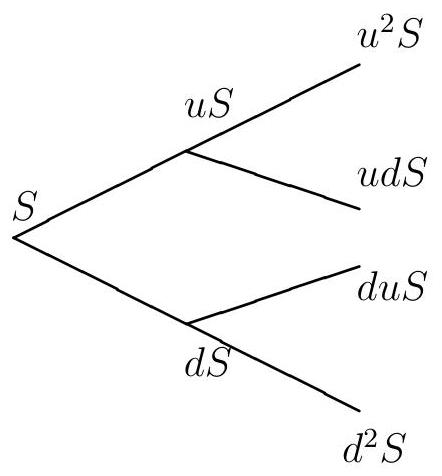
\includegraphics[width=\textwidth]{2024_03_19_5423b86150237379e7feg-055}
% \end{center}

% Noting that the price in the two intermediate branches is the same, we can represent this tree as

% \begin{center}
% 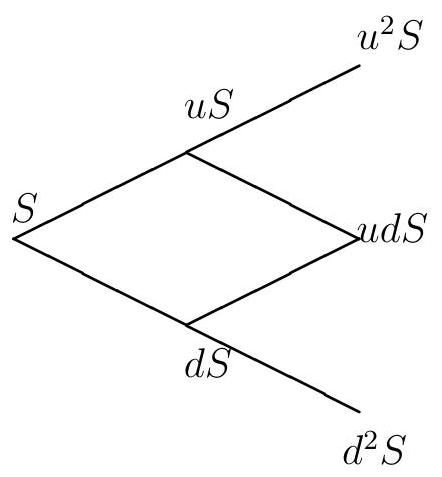
\includegraphics[width=\textwidth]{2024_03_19_5423b86150237379e7feg-056}
% \end{center}

% The binomial tree is thus recombining. After \(T\) periods, it has only \(T+1\) branches instead of \(2^{T}\).

% In the Binomial model markets are complete, since the number of linearly independent securities is equal to the number of nodes one period ahead. Therefore, every option is redundant.

% Pricing a European option is very simple. We first compute the state prices. We next evaluate the option's cash flow \(\left(\max \left(S_{\tau}-X, 0\right)\right.\) for the call, \(\max \left(X-S_{\tau}, 0\right)\) for the put) at the state prices.


% \subsection*{4.2 Portfolio Choice}
% We consider a securities market model with a probability space $(\Omega, \mathcal{F}, P)$, a set of trading dates \(\mathcal{T}=\{0,1, \cdots, T\}\), a filtration \(\mathbb{F}\), and \(N+1\) securities characterized by a dividend process \(\delta\) and a price process \(S\).

% Definition 4.2.3 A consumption plan is an adapted process \(c \in \mathcal{L}^{+}\).

% We consider an investor who consumes over time. The investor's preferences are given by a strictly increasing and continuous utility function \(U: \mathcal{L}^{+} \rightarrow \mathbb{R}\). We will often assume that \(U\) is a time-additive expected utility, i.e.

% \begin{equation*}
% U(c)=E_{0} \sum_{t=0}^{T} u_{t}\left(c_{t}\right) \tag{4.2.1}
% \end{equation*}

% The investor has wealth \(W\) in period 0 .

% Given a consumption plan \(c\), we denote by \(c-W\) the cash flow that is equal to \(c_{t}\) for \(t \geq 1\), and \(c_{0}-W\) for \(t=0\). The cash flow \(c-W\) must be marketable, i.e. must belong to \(M\).

% Definition 4.2.4 A consumption plan \(c\) is feasible iff \(c-W \in M\).

% Setting

% \begin{equation*}
% M+W \equiv\{c: c-W \in M\}
% \end{equation*}

% a consumption plan is feasible iff it belongs to \(M+W\).

% The investor's problem, $(\mathcal{P})$, is

% \begin{equation*}
% \begin{gathered}
% \max _{c} U(c) \\
% c \in \mathcal{L}^{+} \cap(M+W) .
% \end{gathered}
% \end{equation*}

% Definition 4.2.5 A consumption plan \(c\) is optimal iff it solves \(\mathcal{P}\). A trading strategy is optimal iff it finances \(c-W\).

% There are two approaches for solving \(\mathcal{P}\), the martingale approach and the dynamic programming approach. The martingale approach is based on the FTAP and its consequence, the existence of state prices. The dynamic programming approach is the "traditional" approach and is based on stochastic dynamic programming. We will discuss the dynamic programming approach later, in the context of continuous-time models.

% \subsection*{4.2.1 The Martingale Approach: Existence and Characterization}
% We first examine whether \(\mathcal{P}\) has a solution.

% Theorem 4.2.1 \(\mathcal{P}\) has a solution iff there is no arbitrage.

% Proof: Suppose that there is an arbitrage, i.e., a cash flow \(\hat{c} \in \mathcal{L}_{0}^{+} \cap M\). Consider a solution \(c^{*} \in \mathcal{L}^{+} \cap(M+W)\) of \(\mathcal{P}\). Then \(c^{*}+\hat{c} \in \mathcal{L}^{+} \cap(M+W)\). Moreover, since \(U\) is strictly increasing, \(U\left(c^{*}+\hat{c}\right)>U\left(c^{*}\right)\). Therefore, \(c^{*}\) cannot be a solution.

% Suppose that there is no arbitrage. By the FTAP there exists a state price process \(\psi \in \mathcal{L}^{++}\). Consider \(c \in \mathcal{L}^{+} \cap(M+W)\). Since \(c-W \in M\), we have

% \begin{equation*}
% \Psi(c-W)=0 \Rightarrow K_{0} \sum_{t=0}^{T} \psi_{t} c_{t}=W
% \end{equation*}

% Therefore \(c \in B_{\psi, W}\), where

% \begin{equation*}
% B_{\psi, W} \equiv\left\{c: c \in \mathcal{L}^{+}, K_{0} \sum_{t=0}^{T} \psi_{t} c_{t}=W\right\} \tag{4.2.2}
% \end{equation*}

% The set \(B_{\psi, W}\) is compact. Its closed subset \(\mathcal{L}^{+} \cap(M+W)\) is also compact. Since \(U\) is continuous, \(\mathcal{P}\) has a solution.

% Q.E.D.

% Theorem 4.2.1 states that absence of arbitrage is a necessary and sufficient condition for the existence of a solution to \(\mathcal{P}\). That it is a necessary condition is obvious, otherwise the investor could achieve infinite utility. To show that it is a sufficient condition, we use the FTAP and its consequence, the existence of state prices. We then show that a feasible consumption plan must satisfy the constraint

% \begin{equation*}
% K_{0} \sum_{t=0}^{T} \psi_{t} c_{t}=W \tag{4.2.3}
% \end{equation*}

% Equation 4.2 .3 can be interpreted as a static budget constraint similar to the standard budget constraint in consumer theory. Similarly, the set \(B_{\psi, W}\) can be interpreted as a budget set.

% We next obtain a useful characterization of the solution to \(\mathcal{P}\). We assume that \(U\) is differentiable and concave.

% Definition 4.2.6 The gradient of \(U\) at \(c\) is the function \(\nabla U(c)\) defined by

% \begin{equation*}
% \nabla U(c)[\hat{c}] \equiv \lim _{\alpha \rightarrow 0} \frac{U(c+\alpha \hat{c})-U(c)}{\alpha} .
% \end{equation*}

% The function \(\nabla U(c)\) is linear (in \(\hat{c}\) ). It is also strictly increasing since \(U\) is strictly increasing and concave. We can define an adapted process \(R \in \mathcal{L}^{++}\)by

% \begin{equation*}
% \nabla U(c)[\hat{c}]=E_{0} \sum_{t=0}^{T} R_{t} \hat{c}_{t} \tag{4.2.4}
% \end{equation*}

% We refer to the process \(R\) as the Riesz representation of the function \(\nabla U(c)\).

% Proposition 4.2.1 \(c^{*} \in \mathcal{L}^{++}\)is a solution of \(\mathcal{P}\) iff the Riesz representation of \(\nabla U\left(c^{*}\right)\) is a state-price density times a constant \(\lambda>0\).

% Proof: Since \(U\) is differentiable and concave, and since the set \(\mathcal{L}^{+} \cap(M+W)\) is convex, \(c^{*}\) is a solution of \(\mathcal{P}\) iff \(\nabla U\left(c^{*}\right)\left[c-c^{*}\right] \leq 0\) for all \(c \in \mathcal{L}^{+} \cap(M+W)\). Since \(c^{*} \in \mathcal{L}^{++}\), the latter condition is equivalent to \(\nabla U\left(c^{*}\right)[\hat{c}]=0\) for all \(\hat{c} \in M\). This means that the Riesz representation of \(\nabla U\left(c^{*}\right)\) is a SPD times a constant \(\lambda>0\). The constant \(\lambda\) is such that the SPD in period 0 is equal to 1 .

% Q.E.D.

% Note: It is critical that \(c^{*}\) is an interior solution, otherwise Proposition 4.2.1 is not valid, since \(\nabla U\left(c^{*}\right)\left[c-c^{*}\right] \leq 0\) for all \(c \in \mathcal{L}^{+} \cap(M+W)\) does not imply that \(\nabla U\left(c^{*}\right)[\hat{c}]=0\).

% When \(U\) is a time-additive expected utility, the Riesz representation of \(\nabla U(c)\) is the process \(R_{t}=u_{t}^{\prime}\left(c_{t}\right)\). Using proposition 4.2.1, we can write the relations between SPD and security prices as

% \begin{equation*}
% S_{t}=\frac{1}{u_{t}^{\prime}\left(c_{t}^{*}\right)} E_{t}\left(\sum_{s=t+1}^{T} u_{s}^{\prime}\left(c_{s}^{*}\right) \delta_{s}+u_{T}^{\prime}\left(c_{T}^{*}\right) S_{T}\right) \tag{4.2.5}
% \end{equation*}

% or

% \begin{equation*}
% S_{t}=\frac{1}{u_{t}^{\prime}\left(c_{t}^{*}\right)} E_{t}\left[u_{t+1}^{\prime}\left(c_{t+1}^{*}\right)\left(\delta_{t+1}+S_{t+1}\right)\right] \tag{4.2.6}
% \end{equation*}

% Equations (4.2.5 and 4.2.6) relate the investor's optimal consumption to security prices. When studying the investor's portfolio problem, we take security prices as given, and determine the optimal consumption. Then, to compute the optimal portfolio strategy, we simply find a portfolio-consumption strategy replicating the optimal consumption plan, which is always possible in a complete market.

% When studying equilibrium, we sometimes follow the inverse procedure. We take consumption as given, and determine the security prices that make this consumption optimal.

% We refer to equation 4.2 .6 as the Euler equation.

% \subsection*{4.2.2 Complete Markets}
% The characterization of proposition 4.2.1 is particularly useful when markets are complete. Indeed, with complete markets, the SPD is unique. Denoting the SPD by \(\pi\) and the state price process by \(\psi\), we get

% \begin{equation*}
% u_{t}^{\prime}\left(c_{t}^{*}\right)=\lambda \pi_{t}=\lambda \frac{\psi_{t}}{p_{t}} \tag{4.2.7}
% \end{equation*}

% Equation 4.2.7, together with the static budget constraint 4.2.3, fully determine the optimal consumption. (Assuming that \(c^{*} \in \mathcal{L}^{++}\).)

% We determined the optimal consumption using proposition 4.2.1 and the uniqueness of the SPD. A more indirect, and perhaps more intuitive, approach consists in determining the set \(\mathcal{L}^{+} \cap(M+W)\) of feasible consumption plans.

% Lemma 4.2.1 When markets are complete, \(\mathcal{L}^{+} \cap(M+W)=B_{\psi, W}\).

% Proof: In the proof of theorem 4.2 .1 we showed that \(\mathcal{L}^{+} \cap(M+W) \subseteq B_{\psi, W}\), so we only need to show the converse. Consider \(c \in B_{\psi, W}\). Since markets are complete, there exists a trading strategy \(\theta\) that replicates \(c\). Therefore, the cash flow that is equal to \(c_{t}\) for \(t \geq 1\), and \(-\theta_{0} S_{0}\) for \(t=0\), belongs to \(M\). Since

% \begin{equation*}
% -\theta_{0} S_{0}+K_{0} \sum_{t=1}^{T} \psi_{t} c_{t}=0
% \end{equation*}

% and \(c \in B_{\psi, W}\), we have \(c_{0}-W=-\theta_{0} S_{0}\). Therefore, \(c-W \in M\), i.e. \(c \in M+W\). Q.E.D.

% Lemma 4.2.1 implies that the set of feasible consumption plans is the budget set \(B_{\psi, W}\) that corresponds to the state price process \(\psi\). Therefore, the problem \(\mathcal{P}\) is equivalent to the problem

% \begin{equation*}
% \begin{aligned}
% & \max _{c} U(c) \\
% & c \in B_{\psi, W} .
% \end{aligned}
% \end{equation*}

% This "static" problem is the standard problem in consumer theory. The first-order condition of this problem is equation 4.2.7. (Assuming that \(c^{*} \in \mathcal{L}^{++}\).) We denote the static problem by \(\mathcal{P}_{\psi}\). We also denote the maximum values of the problems \(\mathcal{P}\) and \(\mathcal{P}_{\psi}\) by \(U^{*}\) and \(U_{\psi}^{*}\), respectively.

% \subsection*{4.2.3 Incomplete Markets}
% When markets are incomplete, things are more complicated. The SPD is not unique, so proposition 4.2.1 does not fully determine the optimal consumption. Moreover, lemma 4.2.1 does not apply, and thus the set of feasible consumption plans is not a budget set. To determine the optimal consumption, we first study the set of feasible consumption plans. We denote by \(\boldsymbol{\Psi}\) the set of state price processes (which is not a singleton since markets are incomplete).

% Lemma 4.2.2 We have

% \begin{equation*}
% \mathcal{L}^{+} \cap(M+W) \subseteq \cap_{\psi \in \Psi} B_{\psi, W}
% \end{equation*}

% Proof: In the proof of theorem 4.2.1 we showed that if \(\psi\) is a state price process, then \(\mathcal{L}^{+} \cap(M+W) \subseteq B_{\psi, W}\). Since this holds for any \(\psi \in \boldsymbol{\Psi}\), the lemma follows. Q.E.D.

% The set of feasible consumption plans is thus included in the intersection over state price processes of the budget sets corresponding to each process. The converse is also true and left as an exercise.

% We next consider the static problem

% \begin{equation*}
% \begin{gathered}
% \max _{c} U(c) \\
% c \in \cap_{\psi \in \Psi} B_{\psi, W}
% \end{gathered}
% \end{equation*}

% and denote by \(U_{\Psi}^{*}\) its maximum value. We will show that the problem \(\mathcal{P}\) is equivalent to this static problem, and is also equivalent to a "dual" problem.

% Proposition 4.2.2 We have

% \begin{equation*}
% U^{*}=U_{\Psi}^{*}=\inf _{\psi \in \Psi} U_{\psi}^{*}
% \end{equation*}

% Proof: We will show that

% \begin{equation*}
% U^{*} \leq U_{\Psi}^{*} \leq \inf _{\psi \in \Psi} U_{\psi}^{*} \leq U^{*}
% \end{equation*}

% Lemma 4.2.2 implies that \(U^{*} \leq U_{\Psi}^{*}\). We clearly have \(U_{\Psi}^{*} \leq U_{\psi}^{*}\) for all \(\psi \in \boldsymbol{\Psi}\). Therefore,

% \begin{equation*}
% U_{\Psi}^{*} \leq \inf _{\psi \in \Psi} U_{\psi}^{*}
% \end{equation*}

% To show that

% \begin{equation*}
% \inf _{\psi \in \Psi} U_{\psi}^{*} \leq U^{*}
% \end{equation*}

% we assume that the solution \(c^{*}\) of \(\mathcal{P}\) is in \(\mathcal{L}^{++}\). Proposition 4.2.1 implies that the Riesz representation of \(\nabla U\left(c^{*}\right)\) is a SPD times a constant \(\lambda>0\). Denote by \(\psi^{*}\) the associated state price process. Then \(c^{*}\) is the solution to \(\mathcal{P}_{\psi^{*}}\). Therefore,

% \begin{equation*}
% U^{*}=U_{\psi^{*}}^{*} \geq \inf _{\psi \in \boldsymbol{\Psi}} U_{\psi}^{*} .
% \end{equation*}

% Proposition 4.2.2 implies that the problem \(\mathcal{P}\) is equivalent to the static problem. The problem \(\mathcal{P}\) is also equivalent to a dual problem, which consists of (i) solving the complete markets problem for each \(\psi \in \boldsymbol{\Psi}\) and (ii) minimizing the maximum value \(U_{\psi}^{*}\) over \(\boldsymbol{\Psi}\). The dual problem is sometimes simpler to solve than \(\mathcal{P}\).

% Example 4.2.2 Suppose that \(\Omega=\left\{\omega_{1}, \omega_{2}, \omega_{3}\right\}, \mathcal{F}=2^{\Omega}, T=1, \mathcal{F}_{0}=\{\emptyset, \Omega\}, \mathcal{F}_{1}=\mathcal{F}\), and there are 2 securities 0 and 1 , with time 0 and 1 prices given by

% \begin{center}
% \begin{tabular}{|l|c|c|c|c|}
% \hline
%  & Time 0 & \multicolumn{3}{|c|}{Time 1} \\
% \hline
%  &  & State \(\omega_{1}\) & State \(\omega_{2}\) & State \(\omega_{1}\) \\
% \hline
% Security 0 & 1 & 1 & 1 & 1 \\
% \hline
% Security 1 & 2 & 3 & 2 & 1 \\
% \hline
% \end{tabular}
% \end{center}

% Suppose also that

% \begin{equation*}
% U(c)=\frac{1}{3}\left(\log \left(c\left(\omega_{1}, 1\right)\right)+\log \left(c\left(\omega_{2}, 1\right)\right)+\log \left(c\left(\omega_{3}, 1\right)\right)\right)
% \end{equation*}

% The set of feasible consumption plans is defined by

% \begin{equation*}
% \begin{aligned}
% & c\left(\omega_{1}, 1\right)=\theta^{0}(\omega, 0)+3 \theta^{1}(\omega, 0) \geq 0, \\
% & c\left(\omega_{2}, 1\right)=\theta^{0}(\omega, 0)+2 \theta^{1}(\omega, 0) \geq 0,
% \end{aligned}
% \end{equation*}

% and

% \begin{equation*}
% c\left(\omega_{3}, 1\right)=\theta^{0}(\omega, 0)+\theta^{1}(\omega, 0) \geq 0
% \end{equation*}

% where

% \begin{equation*}
% W=\theta^{0}(\omega, 0)+2 \theta^{1}(\omega, 0)
% \end{equation*}

% We can write this set as

% \begin{equation*}
% c\left(\omega_{2}, 1\right)=W, \quad \frac{1}{2}\left(c\left(\omega_{1}, 1\right)+c\left(\omega_{3}, 1\right)\right)=W, \quad c(\omega, 1) \geq 0
% \end{equation*}

% Maximizing \(U\) over this set, we find \(c(\omega, 1)=W\). This is the solution to \(\mathcal{P}\).

% The solution to \(\mathcal{P}_{\psi}\) is

% \begin{equation*}
% c(\omega, 1)=\frac{W}{3 \psi(\omega, 1)}
% \end{equation*}

% Therefore,

% \begin{equation*}
% U_{\psi}^{*}=-\frac{1}{3}\left(\log \left(\psi\left(\omega_{1}, 1\right)\right)+\log \left(\psi\left(\omega_{2}, 1\right)\right)+\log \left(\psi\left(\omega_{3}, 1\right)\right)\right)+\log W
% \end{equation*}

% Minimizing \(U_{\psi}^{*}\) over the set

% \begin{equation*}
% \Psi=\left\{\left(1, \alpha\left(\frac{1}{2}, 0, \frac{1}{2}\right)+(1-\alpha)(0,1,0)\right): \alpha \in(0,1)\right\}
% \end{equation*}

% we get \(\alpha=2 / 3\), i.e., \(\psi(\omega, 1)=1 / 3\) and \(c(\omega, 1)=W\).




\end{document}